% !TeX encoding = UTF-8
% !TeX program = xelatex

% FIXME:
% ~~hyperref \autoref seems to jump to a wrong theorem occasionally~~
%     very likely due to (sub)section resetting ref counter, should be solved with hyperref option hypertexnames=false
% changes \listofchanges does not seem to respect draft/final options
% the current way of controlling package option draft/final is VERY hacky

% content control
% (un)comment these lines to control draft/final version
\newif\ifIsDraft
\IsDrafttrue
\IsDraftfalse

\newif\ifShowCommittee
\ShowCommitteetrue
% \ShowCommitteefalse

\newif\ifShowAbstract
\ShowAbstracttrue
% \ShowAbstractfalse

\newif\ifShowAcknowledgment
\ShowAcknowledgmenttrue
% \ShowAcknowledgmentfalse

\ifIsDraft
\documentclass[
    a4paper,
    11pt,
    twoside,
    draft
]{article}
\else
\documentclass[
    a4paper,
    11pt,
    twoside,
    final
]{article}
\fi


% for editing
\ifIsDraft
\usepackage[
    deletedmarkup=xout,
    commentmarkup=uwave,
    draft
]{changes}
\else
\usepackage[
    deletedmarkup=xout,
    commentmarkup=uwave,
    final
]{changes}
\fi
% ``changes'' package provides commands:
%     \added[id=authorId, comment={commentContent}]{new text...}
%     \deleted[id=authorId, comment={commentContent}]{old text...}
%     \replaced[id=authorId, comment={commentContent}]{new text...}{old text...}
%     \highlight[id=authorId, comment={commentContent}]{highlight text...}
%     \comment[id=authorId]{comment...}
% register your name with the command:
%     \definechangesauthor[name={name}]{displayed abbreviation}
% see doc: http://mirrors.ctan.org/macros/latex/contrib/changes/changes.english.pdf
\definechangesauthor[name={KF Chan}]{KF}

% chinese
\usepackage{xeCJK}
% \setCJKmainfont[AutoFakeBold=1]{STKaiti}
% \setCJKmainfont[AutoFakeBold=1]{DFKai-SB}
% \setCJKmainfont[AutoFakeBold=1]{KaiTi}
\setCJKmainfont[AutoFakeBold=1]{TW-Kai}
\setCJKmonofont{Latin Modern Mono}  % silence warning about unknown CJKttdefault

% page config
% \usepackage[margin=1in]{geometry}
\usepackage[margin=1in]{geometry}
% \geometry{left=2.5cm,right=2.5cm,top=2.5cm,bottom=2.5cm}
\usepackage{setspace}
\setstretch{1.5} % line spacing multiplier, using Feng Zhou's spacing

% math stuff
\usepackage{mathtools}  % loads amsmath
\usepackage{amssymb}
\usepackage{amsthm, thmtools}
\usepackage{mathrsfs}

% thm environments with amsthm and thmtools
\declaretheorem[parent=section]{theorem}
\declaretheorem[parent=section]{lemma}
\declaretheorem[sibling=lemma]{corollary}
\declaretheorem[parent=section, style=definition]{definition}
\declaretheorem[parent=section, style=remark]{remark}
\declaretheorem[style=remark]{observation}
\declaretheorem{conjecture}


% biblo
\usepackage[
    sorting=nyt,
    backend=biber,
    style=trad-abbrv,
    sortcites
]{biblatex}
\addbibresource{thesis-ref.bib}

% writing assist
\usepackage[
    obeyDraft
]{todonotes}
\setuptodonotes{inline, inlinepar, color=green!33}
\ifIsDraft
% \usepackage{showkeys}
\fi
% \usepackage{refcheck}  % appears unreliable, use the python script instead

% misc
\usepackage[en-US]{datetime2}  % for date
\DTMsavenow{compileTimeTimestamp}
\usepackage{tikz}
\usetikzlibrary{intersections, calc, arrows.meta, angles, quotes, through}
% \usepackage{graphicx}
% \usepackage{footmisc}
\usepackage[
    linktocpage,
    %     colorlinks=true,
    %     linkcolor=blue,
    final=true,  % ignore doc class setting
    hypertexnames=false
]{hyperref}
% umm
% \usepackage{sty/usefulmathmacro}
\usepackage{usefulmathmacro}  % make sure that editor autocomplete works well

% document specific macros
\newlength{\writingPlaceholderWidth}
\ProvideDocumentCommand{\writingPlaceholder}{O{?????}}{
    \settowidth{\writingPlaceholderWidth}{#1}
    \hspace{-9pt}
    \todo[noinlinepar, inlinewidth={\writingPlaceholderWidth + 9pt}]{#1}
    \,
}
\ProvideDocumentCommand{\alignspacing}{}{\hphantom{\;=\;}}
\ProvideDocumentCommand{\resCoeff}{}{e_\mathrm{res}}
\ProvideDocumentCommand{\fourier}{}{\mathcal{F}}
\ProvideDocumentCommand{\probMeasureSpace}{O{0}}{P^{#1}}
\ProvideDocumentCommand{\karchSpace}{m}{\mathcal{K}^{#1}}
\ProvideDocumentCommand{\toscaniMetric}{m m}{\norm{#1}_{#2}}
\ProvideDocumentCommand{\morimotoSpace}{m}{\mathcal{M}^{#1}}
\ProvideDocumentCommand{\morimotoMetric}{m m}{\norm{#1}_{\mathcal{M}^{#2}}}
\ProvideDocumentCommand{\nonnegRadon}{}{\mathscr{M}^+}
\ProvideDocumentCommand{\compactRR}{}{\RR_c}
\ProvideDocumentCommand{\measureNorm}{m}{\norm{#1}_{\mathscr{M}}}
\ProvideDocumentCommand{\momentNorm}{m m}{\norm{#1}_{1, #2}}
\DeclareMathOperator{\lipConst}{Lip}

% preamble
\title{
   Self-similar Behavior of Boltzmann Equation under Shearing Effect
}
\author{Chan, Kam Fai}
\date{}

% doc content
\begin{document}

\begin{titlepage}
    \begin{center}
        {\Large\textbf {Self-similar Behavior of Boltzmann Equation\\ under Shearing Effect}}\\[2.4cm]
        {\normalsize\bf CHAN, Kam Fai}\\[2.5cm]
        {\normalsize A Thesis Submitted in Partial Fulfillment}\\[0.5cm]
        {\normalsize of the Requirements for the Degree of}\\[0.5cm]
        {\normalsize Doctor of Philosophy}\\[0.5cm]
        {\normalsize in}\\[0.5cm]
        {\normalsize Mathematics}\\[5cm]
        {\normalsize The Chinese University of Hong Kong}\\[0.5cm]
        {\normalsize {\DTMenglishmonthname{\DTMfetchmonth{compileTimeTimestamp}} \DTMfetchyear{compileTimeTimestamp}}}
    \end{center}
\end{titlepage}


\ifShowCommittee
\begin{titlepage}
    \begin{center}
        {\Large\textbf{\underline{Thesis Assessment Committee}}}\\[2.4cm]
        {\normalsize Professor LUO Chenyun (Chair)}\\[0.5cm]
        {\normalsize Professor DUAN Renjun (Thesis Supervisor)}\\[0.5cm]
        {\normalsize Professor YU Yong (Committee Member)}\\[0.5cm]
        {\normalsize Professor LUO Tao (External Examiner)}\\[0.5cm]
    \end{center}
\end{titlepage}
\fi  % \ifShowCommittee

\ifShowAbstract
\section*{Abstract}
% \begin{abstract}
    The Boltzmann equation is a fundamental equation in the study of rarefied gas dynamics. While there are vast progresses on the equation on both spatially homogeneous and inhomogeneous cases, there are relatively few results on the case where an external anisotropic shearing force is applied on the gas, despite the importance of such model describing the class of homoenergetic solutions of the equation. Due to the rotational effect introduced from such shearing force, specialized methods are required to analyze the equation, and most existing results are obtained with perturbation method near the isotropic case. There is yet a satisfying theory, mirroring the extensive theory on isotropic Boltzmann equation, to fully analyze the behavior under such anisotropic force.

    In this thesis, we will study the behavior of the solutions of the Boltzmann equation with Maxwellian kernel under such shearing force. In particular, we will investigate the self-similar behavior that emerges from the shear flow, and analyze the long-time behavior of such solution in the Fourier framework. Moreover, we will give a detail description of the behavior of such self-similar profile in the specific case where the gas is under the effect of the Uniform Shear Flow (USF).
% \end{abstract}

\clearpage

\section*{摘要}
% \renewcommand{\abstractname}{摘要}
% \begin{abstract}
    在研究稀疏氣體動力學中,玻爾茲曼方程有著無可比擬的地位。在空間齊性及空間非齊性的經典前提下,對應方程的解的行為均有大量理論結果。然而,同氣體受到非各向同性的剪切力影響時,目前對於相關解的行為卻所知甚少。儘管這種剪切力與均能流解 (homogenergetic solution) 的行為有著密切關係,在剪切力帶來的影響下,已有的手段難以獲得與經典玻爾茲曼方程理論相似的結果。因此,目前已有的結果大多來源於對無剪切力方程的微擾分析。

    在此論文中,我們將在麥克斯韋碰撞核的假定下研究相關玻爾茲曼方程解的行為,並會討論由剪切力所帶來的自相似解結構,及在對應傅立葉空間中分析相關解在大時間尺度下的漸近行為。我們亦會詳細討論由均勻剪切流 (uniform shear flow, USF) 所帶來的影響。
% \end{abstract}

\clearpage
\fi  % \ifShowAbstract

\ifShowAcknowledgment
\section*{Acknowledgment}

First and foremost, I would like to thank my supervisor, Prof.\ Renjun Duan, for introducing me to the topic of Boltzmann equation and the various research projects, for his emphasis on independent researching propels me forward in my study, and for giving me the great degree of freedom to work on my ideas, far more than a PhD student could ask for.
I am forever grateful for his guidance and teaching, and for providing such nourishing environment for researches.

I would also like to thank Prof.\ Shuaikun Wang for our discussions on the infinite energy solutions, for his critical insights and suggestions have enabled a new perspective on the problem, without which certain parts of this thesis would not be possible.

I am greatly indebted to my long-time colleagues and friends, Zongguang Li, Zhiwen Zhang, Junhao Zhang, Kunlun Qi, and the many people from the Department who have kindly shared with me their intelligence and perspectives.
While we do not necessarily work on the same problem or even be in the same field, I have learned far more from them than I could have expected, and their words have been a constant source of ideas and encouragements.

Last but not least, I would like to thank my family for their constant and unconditional support throughout the years of my studies.
Without them, it would be impossible for me to make any progress, let alone complete this work.


\clearpage

\fi  % \ifShowAcknowledgment

\tableofcontents

\ifIsDraft
\listoftodos
\listofchanges
\fi

\clearpage
\section{Introduction}

The focus of this thesis is the analysis on the solution to the spatially homogeneous Boltzmann equation in the Euclidean space, under the effect of an external shearing force, and correspondingly its self-similar behavior.

\subsection{Boltzmann Equation}
% The major focus of this paper is the Boltzmann equation

% \todo{more origin about the equation? e.g.\ stosszahlansatz, bbgky (too irrelevant?)}

The spatially homogeneous Boltzmann equation on \( \RR^d \) \( (d \geq 2) \) \cite{Cercignani88BEI},
\begin{equation} \label{equ:spatialHomoBoltzmann}
    \pd{t} f = Q(f, f),
\end{equation}
describes the dynamics of rarefied gas molecules via the one-particle distribution function
\begin{equation*}
    f(t, v) : [0, \infty) \times \RR^d \to [0, \infty)
\end{equation*}
that represents the density of the molecules at the given time \( t \geq 0 \) with the given velocity \( v  \in \RR^d \).
The operator on the right-hand side,
\begin{equation} \label{equ:boltzmannCollisionOp_strongForm}
    Q(g, f)
    \coloneqq \integration{v_*}{\RR^d}{}{
        \integration{\sigma}{S^{d - 1}}{}{
            B\parenth*(v - v_*, \normalized{v - v_*} \cdot \sigma) (f' g_*' - f g_*)
        }
    },
\end{equation}
is the Boltzmann collision operator, where \( B(z, \cos\theta) \geq 0 \) is the collision kernel determined by the interactions between the molecules, and, in \( \sigma \)-representation,
\begin{equation} \label{equ:postCollisionVelocities}
\begin{aligned}
    v'
    &= \frac{v + v_*}{2} + \frac{1}{2} \abs{v - v_*} \sigma, \\
    v_*'
    &= \frac{v + v_*}{2} - \frac{1}{2} \abs{v - v_*} \sigma,
\end{aligned}
\end{equation}
are the post-collision velocities, with the common shorthand notation
\begin{equation*}
    f'(t) = f(t, v'), \quad
    f_*(t) = f(t, v_*), \quad
    f_*'(t) = f(t, v_*').
\end{equation*}
Governed by the law of elastic collisions, the velocity variables satisfy the classic relations
\begin{align*}
    v_* + v_*' &= v + v_*, \\
    \abs{v_*}^2 + \abs{v_*'}^2 &= \abs{v}^2 + \abs{v_*}^2,
\end{align*}
which, respectively, correspond to the conservation of particle momentum and energy for each collision.
It is typical to also define an auxiliary variable \( \theta \) to be the derivation angle between \( v - v_* \) and \( \sigma \), such that
\begin{equation*}
    \cos\theta = \normalized{v - v_*} \cdot \sigma.
\end{equation*}

It is also common to write the post-collision velocities \eqref{equ:postCollisionVelocities} in the \( \omega \)-representation, in which they are represented as
\begin{align*}
    v'
    &= v - ((v - v_*) \cdot \omega) \omega, \\
    v_*'
    &= v_* + ((v - v_*) \cdot \omega) \omega
\end{align*}
with \( \omega \in S^{d - 1} \), and to also denote the angle between \( v - v_* \) and \( \omega \) as \( \theta \), so that
\begin{equation*}
    \cos\theta = \normalized{v - v_*} \cdot \omega.
\end{equation*}
To avoid confusion, let us denote for the moment this angle as \( \theta_\omega \), and the deviation angle in \( \sigma \)-representation as \( \theta_\sigma \) instead.
In such case, the corresponding collision kernel \( B_\omega \) and the kernel \( B_\sigma \) in \( \sigma \)-representation \eqref{equ:boltzmannCollisionOp_strongForm} differs by a factor from the change in variables:
\begin{equation*}
    B_\omega(z, \cos\theta_\omega)
    = 2^{d - 1} \abs{\normalized{z} \cdot \omega} B_\sigma(z, \cos\theta_\sigma).
\end{equation*}
It should be noted that, in \( \omega \)-representation, each pair of post-collision velocities \( (v', v_*') \) is covered twice when enumerating \( \omega \in S^{d - 1} \), by \( \omega \) and by \( -\omega \).

For consistency, we will use solely the \( \sigma \)-representation, unless explicitly stated otherwise.

\begin{figure}[h]
    \centering
    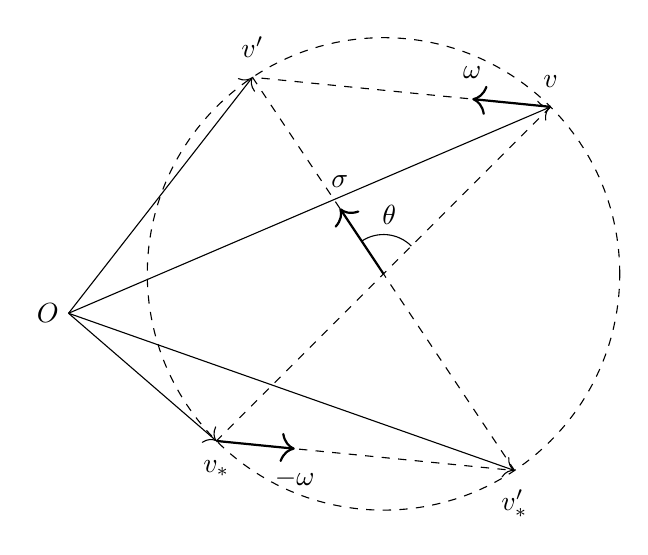
\begin{tikzpicture}
        \coordinate (mid) at (0, 0) {};
        \coordinate [label=left:\( O \)] (orig) at (-4, -0.5) {};
        \path [name path=pre] (-3, -3) -- (3, 3);
        \path [name path=post] (2, -3) -- (-2, 3);
        \path [draw, dashed, name path=circ] (mid) circle [radius=3];
        \path [name intersections={of=pre and circ, by={v, vstar}}]
            node [label=\( v \)] at (v) {}
            node [label=below:\( v_* \)] at (vstar) {};
        \path [name intersections={of=post and circ, by={vprime, vprimestar}}]
            node [label=\( v' \)] at (vprime) {}
            node [label=below:\( v'_* \)] at (vprimestar) {};
        \draw [dashed] (v) -- (vstar);
        \draw [dashed] (vprime) -- (vprimestar);
        \draw [thick, arrows={->[scale=1.5]}] (mid) -- ($(mid)!1cm!(vprime)$)
            node [label=above:\( \sigma \)] {};
        \path [draw, arrows={->[scale=1.5]}] (orig) -- (v);
        \path [draw, arrows={->[scale=1.5]}] (orig) -- (vstar);
        \path [draw, arrows={->[scale=1.5]}] (orig) -- (vprime);
        \path [draw, arrows={->[scale=1.5]}] (orig) -- (vprimestar);
        \pic [draw, "$\theta$", angle eccentricity=1.5] {angle = v--mid--vprime};
        \draw [dashed] (v) -- (vprime);
        \draw [thick, arrows={->[scale=1.5]}] (v) -- ($(v)!1cm!(vprime)$) node [label=above:\( \omega \)] {};
        \draw [dashed] (vstar) -- (vprimestar);
        \draw [thick, arrows={->[scale=1.5]}] (vstar) -- ($(vstar)!1cm!(vprimestar)$) node [label=below:\( -\omega \)] {};
    \end{tikzpicture}
    \caption{Geometrical representation of the pre- and post-collision velocity variables.}
\end{figure}

For the intermolecular interactions induced by a power-law potential \( U(r) \propto r^{-s} \), the collision kernel can be shown to be of the form
\begin{equation*}
    B(z, \cos\theta)
    = \Phi(z) \; b(\cos\theta)
\end{equation*}
where \( \Phi(z) = \abs{z}^\gamma \) is the kinetic part, and \( b(\cos\theta) \geq 0 \) is the angular part of the collision kernel, with parameter \( \gamma \in (-d, 1] \).
The cases \( \gamma \in (-d, 0) \), \( \gamma = 0 \), \( \gamma \in (0, 1] \) are called, respectively, soft potential, Maxwell molecule, and hard potential.
In the specific case of Maxwell molecule, the collision kernel has no dependency on the modulus of the velocity difference, and the behavior of the collision operator depends solely on the angular part \( b \).

In the most typical case of three-dimensional space \( d = 3 \), for the kernel induced by a power-law potential \( U(r) \propto r^{-s} \) of order \( s \), we have
\begin{align*}
    \gamma
    &= \frac{s - 5}{s - 1}, \\
    b(\cos\theta) \sin\theta
    &\sim \theta^{-(2 s + 1)} \quad \mathrm{on\ } \theta \to 0,
\end{align*}
and the specific case of power-law potential of order \( s = 5 \) yields a Maxwell molecule.
% \todo{high dimension description?}

% \todo{more descriptions about hard potential and soft potential}

For simplicity in our analysis, we will focus solely on the case of Maxwell molecule, that is the specific case where \( B(z, \cos\theta) = b(\cos\theta) \) depends only on the derivation angle.

As the angular part \( b(\cos\theta) \) of such physical collision kernel has a non-integrable singularity at \( \theta = 0 \), it is common to additionally pose Grad's cutoff assumption \cite{Grad58PKT}
\begin{equation*}
    0 \leq b(\cos\theta) \sin^{d - 2}\theta \lesssim \abs{\cos\theta}
\end{equation*}
so that \( b_0 \coloneqq \integration{\sigma}{S^{d - 1}}{}{b(\cos\theta)} < \infty \), which removes certain difficulties that arise in the analysis due to the singularity.
Kernels with such property are referred to as cutoff kernels, and those which the angular part is not integrable are non-cutoff kernels.
% \todo{more description on non-cutoff}

One important feature of cutoff kernel is that the collision operator can be split into gain part and loss part,
\begin{equation*}
    Q(g, f)
    = Q^+(g, f) - Q^-(g, f),
\end{equation*}
where the gain part is
\begin{equation*}
    Q^+(g, f)
    \coloneqq \integration{v_*}{\RR^d}{}{
        \integration{\sigma}{S^{d - 1}}{}{
            B(v - v_*, \cos\theta) f' g_*'
        }
    },
\end{equation*}
and, assuming that the collision kernel is induced from a power-law interaction, the loss part is
\begin{align*}
    Q^-(g, f)
    &\coloneqq \integration{v_*}{\RR^d}{}{
        \integration{\sigma}{S^{d - 1}}{}{
            B(v - v_*, \cos\theta) f g_*
        }
    } \\
    &= \parenth*(\integration{\sigma}{S^{d - 1}}{}{b\parenth*(\cos\theta)}) \parenth*(\integration{v_*}{\RR^d}{}{\abs{v - v_*}^\gamma g_*}) f \\
    &= b_0 \parenth*(\integration{v_*}{\RR^d}{}{\abs{v - v_*}^\gamma g_*}) f.
\end{align*}

A typical approach to handle the collision operator is to consider the operator in Maxwell's weak form \cite{Villani02RMT}:
on appropriate test function \( \varphi(v) \),
\begin{equation} \label{equ:boltzmannCollisionOp_weakForm}
\begin{aligned}
    \integration{v}{\RR^d}{}{\varphi Q(f, f)}
    &= \iiint B(v - v_*, \cos\theta) \varphi (f' f_*' - f f_*) \dd{\sigma; v_*; v} \\
    &= \iiint B(v - v_*, \cos\theta) f f_* (\varphi' - \varphi) \dd{\sigma; v_*; v} \\
    &= \frac{1}{2} \iiint B(v - v_*, \cos\theta) f f_* (\varphi' + \varphi_*' - \varphi - \varphi_*) \dd{\sigma; v_*; v}
\end{aligned}
\end{equation}
where the second and the last equalities are due to the change of variables
\begin{equation*}  % \label{equ:prePostChangeVar}
    (v, v_*, \sigma) \mapsto \parenth*(v', v_*', \normalized{v - v_*})
\end{equation*}
having unit Jacobian.
As it can be seen from the weak form, if the test function \( \varphi \) satisfies
\begin{equation*}
    \varphi' + \varphi_*' = \varphi + \varphi_*,
\end{equation*}
\eqref{equ:boltzmannCollisionOp_weakForm} implies \( \pd{t} \int \varphi f = \int \varphi Q(f, f) = 0 \), indicating that \( \int \varphi f \) is constant in time throughout the evolution.
In particular, as it is trivial to verify that \( 1, v, \abs{v}^2 \) satisfy this relation, we obtain the classic conservation laws on the macroscopic quantities
\begin{alignat*}{2}
    \od{t} \integration{v}{\RR^d}{}{f} &= 0 & \quad & \text{(conservation of mass)}, \\
    \od{t} \integration{v}{\RR^d}{}{v f} &= 0 & \quad & \text{(conservation of momentum)}, \\
    \od{t} \integration{v}{\RR^d}{}{\frac{1}{2} \abs{v}^2 f} &= 0 & \quad & \text{(conservation of energy)}.
\end{alignat*}
Furthermore, under some very weak conditions \cite{Cercignani88BEI}, it can be shown that these are the only functions that have such properties.

If we take \( \varphi = \ln f \), then formally on the quantity \( H(t) = \integration{v}{}{}{f \ln f} \), which up to the sign is the entropy of the distribution \( f \), we have the celebrated H-theorem \cite{CercignaniLampis81HTP},
\begin{align*}
    \od{t} H
    &= \od{t} \int f \ln f \\
    &= \int (1 + \ln f) \pd{t} f \\
    &= \frac{1}{2} \iiint B(v - v_*, \cos\theta) f f_* (\ln f' + \ln f_*' - \ln f - \ln f_*) \\
    &= \frac{1}{2} \iiint B(v - v_*, \cos\theta) f f_* \parenth*(1 - \frac{f' f_*'}{f f_*} + \ln \frac{f' f_*'}{f f_*}) \\
    &\leq 0,
\end{align*}
due to the conservation of mass and the elementary inequality \( 1 - x + \ln x \leq 0 \) on \( x \geq 0 \), and equality holds if and only if \( f' f_*' = f f_* \).
Under suitable assumptions \cite{Cercignani88BEI}, this implies that the Maxwellian distribution
\begin{equation}  \label{equ:statMaxwellDistribution}
    f(v)
    = \frac{\rho}{(2 \pi T)^{d / 2}} \exp\parenth*(-\frac{1}{2 T} \abs{v - u}^2),
\end{equation}
with constant macroscopic mass \( \rho \geq 0 \), bulk velocity \( u \in \RR^d \), and macroscopic temperature \( T > 0 \), is the stationary solution to \eqref{equ:spatialHomoBoltzmann}.

As we are considering the case where the collision kernel is Maxwell molecule \( B(z, \cos\theta) = b(\cos\theta) \), on test function \( \varphi(v, k) = e^{-i k \cdot v} \), we obtain from \eqref{equ:boltzmannCollisionOp_weakForm} the Bobylev equation \cite{Bobylev75FTM, Bobylev84ESN, Bobylev88TNS}
\begin{equation} \label{equ:spatialHomoBobylev}
    \pd{t} \varphi = \widehat{Q}(\varphi, \varphi)
\end{equation}
on the Fourier transform \( \varphi(t, k) = (\fourier f)(t, k) \coloneqq \int e^{-i k \cdot v} f(t, v) \dd{v} \), where the Bobylev collision operator on the right-hand side is defined as
\begin{equation*}
    \widehat{Q}(\varphi, \varphi)
    \coloneqq \integration{\sigma}{S^{d - 1}}{}{
        b(\cos\theta) (\varphi^+ \varphi^- - \varphi(0) \varphi)
    },
\end{equation*}
with post-collision frequency variables
\begin{equation} \label{equ:postCollisionFrequencies}
\begin{aligned}
    k^+
    &= \frac{1}{2} k + \frac{\abs{k}}{2} \sigma, \\
    k^-
    &= \frac{1}{2} k - \frac{\abs{k}}{2} \sigma
    = k - k^+,
\end{aligned}
\end{equation}
using a similar shorthand notation as the density function
\begin{equation*}
    \varphi^+(t) = \varphi(t, k^+),
    \quad
    \varphi^-(t) = \varphi(t, k^-).
\end{equation*}
Note that while the usual Boltzmann collision operator is a \( (2 d - 1) \)-fold integral, the Bobylev collision operator is only a \( (d - 1) \)-fold integral, at the cost of losing Maxwell's weak form.

Similar to the velocities, it is also possible to write the post-collision frequencies in the \( \omega \)-representation as
\begin{align*}
    k^+
    &= k - (k \cdot \omega) \omega, \\
    k^-
    &= (k \cdot \omega) \omega,
\end{align*}
and each pair of post-collision frequencies \( (k^+, k^-) \) is covered by both \( \omega \) and \( -\omega \).

\begin{figure}[h]
    \centering
    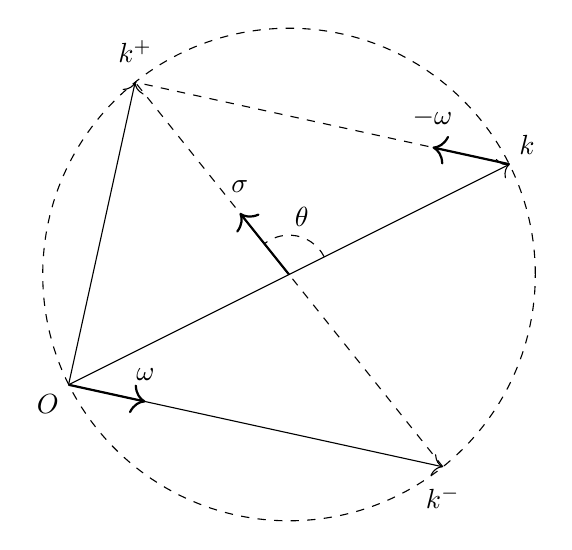
\begin{tikzpicture}
        \coordinate (mid) at (0, 0);
        \coordinate [label=above right:\( k \)] (k) at (2.8, 1.4);
        \coordinate [label=below left:\( O \)] (orig) at ($-1*(k)$);
        \coordinate (kplusdir) at (2, -2.5);
        \node [draw, dashed, circle through={(k)}, name path=circ] at (mid) {};
        \path [name path=kline] (orig) -- (k);
        \path [name path=post] (kplusdir) -- ($-1*(kplusdir)$);
        \path [draw, arrows={->[scale=1.5]}] (orig) -- (k);
        \path [name intersections={of=post and circ, by={kplus, kminus}}]
            node [label=above:\( k^+ \)] at (kplus) {}
            node [label=below:\( k^- \)] at (kminus) {};
        \path [draw, dashed] (kminus) -- (kplus);
        \draw [thick, arrows={->[scale=1.5]}] (mid) -- ($(mid)!1cm!(kplus)$)
            node [label=above:\( \sigma \)] {};
        \draw [arrows={->[scale=1.5]}] (orig) -- (kplus);
        \draw [arrows={->[scale=1.5]}] (orig) -- (kminus);
        \pic [draw, dashed, "$\theta$", angle eccentricity=1.5] {angle = k--mid--kplus};
        \draw [thick, arrows={->[scale=1.5]}] (orig) -- ($(orig)!1cm!(kminus)$) node [label=above:\( \omega \)] {};
        \draw [dashed] (k) -- (kplus);
        \draw [thick, arrows={->[scale=1.5]}] (k) -- ($(k)!1cm!(kplus)$) node [label=above:\( -\omega \)] {};
    \end{tikzpicture}
    \caption{Geometrical representation of the pre- and post-collision frequency variables.}
\end{figure}


Due to the conservation of mass, it is common to assume that \( \int f(t) \dd{v} = 1 \), in which case \( f(t) \) is a probability density, and Bobylev equation is an equation on its characteristic function (up to a sign of the imaginary unit).

In the specific case where \( b \) is a cutoff kernel with \( b_0 = \int b(\cos\theta) \dd{\sigma} < \infty \), the Bobylev collision operator can also be split into gain part and loss part
\begin{equation*}  \label{def:bobylevOp_split}
\begin{aligned}
    \widehat{Q}(\varphi, \varphi)
    &= \widehat{Q}^+(\varphi, \varphi) - \widehat{Q}^-(\varphi, \varphi), \\
    \widehat{Q}^+(\psi, \varphi)
    &\coloneqq \integration{\sigma}{S^{d - 1}}{}{
        b(\cos\theta) \varphi^+ \psi^-
    }, \\
    \widehat{Q}^-(\psi, \varphi)
    &\coloneqq \integration{\sigma}{S^{d - 1}}{}{
        b(\cos\theta) \psi(0) \varphi
    }
    = b_0 \psi(0) \varphi.
\end{aligned}
\end{equation*}

In the study of the equations, the following constants related to the kernel are commonly used in describing certain behaviors of the solutions \cite{Bobylev20KEV}: for \( n \in \NN \), \( p \geq 0 \),
\begin{equation}  \label{def:kernelConstants}
\begin{aligned}
    b_n
    &\coloneqq \integration{\sigma}{S^{d - 1}}{}{b(\cos\theta) \; (\cos\theta)^n}, \\
    \lambda_p
    &\coloneqq \integration{\sigma}{S^{d - 1}}{}{
        b(\cos\theta) \parenth*(1 - \frac{\abs{k^+}^p + \abs{k^-}^p}{\abs{k}^p})
    }, \\
    \mu_p
    &\coloneqq \lambda_p / p,
\end{aligned}
\end{equation}
which could be infinite if the kernel is non-cutoff.
With the collision law, the independence of \( \lambda_p \) from variable \( k \) can be noted by rewriting the definition in an equivalent form
\begin{equation*}
    \lambda_p
    = \integration{\sigma}{S^{d - 1}}{}{
        b(\cos\theta) \parenth*(1 - \abs{\cos\frac{\theta}{2}}^p - \abs{\sin\frac{\theta}{2}}^p)
    },
\end{equation*}
noting that \( \abs{k^+} = \abs{k} \cos\frac{\theta}{2} \) and \( \abs{k^-} = \abs{k} \sin\frac{\theta}{2} \), with \( \theta / 2 \in [0, \pi / 2] \).

It is easy to see from the definition that \( p \mapsto \lambda_p \) is non-decreasing, with \( -b_0 = \lambda_0 \leq \lambda_p \leq b_0 \), and \( \lambda_2 = 0 \). Furthermore,
\begin{align*}
    \od{p} \mu_p
    &= p^{-1} \parenth*(\od{p} \lambda_p - \mu_p) \\
    &= p^{-1} \integration{\sigma}{S^{d - 1}}{}{
        b(\cos\theta)
        \parenth(\abs{c}^p (1 - p \ln\abs{c}) + \abs{s}^p (1 - p \ln\abs{s}) - 1)
    }
\end{align*}
with \( c = \cos\frac{\theta}{2}, s = \sin\frac{\theta}{2} \), and the integrand is non-increasing in \( p \) as
\begin{align*}
    &\alignspacing
    \pd{p} \parenth*(\abs{c}^p (1 - p \ln\abs{c}) + \abs{s}^p (1 - p \ln\abs{s}) - 1) \\
    &= -p \parenth*(\abs{c}^p (\ln\abs{c})^2 + \abs{s}^p (\ln\abs{s})^2) \\
    &\leq 0,
\end{align*}
and takes value \( \abs{c}^2 (1 - 2 \ln\abs{c}) + \abs{s}^2 (1 - 2 \ln\abs{s}) - 1 = -2 (\abs{c}^2 \ln\abs{c} + \abs{s}^2 \ln\abs{s}) \geq 0 \) at \( p = 2 \), which implies \( \mu_p \) is increasing on \( p \in [0, 2] \).

\begin{figure}[h]
    \centering
    \includegraphics[width=0.48\textwidth]{lambdap_constkernel.png} \hfill
    \includegraphics[width=0.48\textwidth]{mup_constkernel.png}
    \caption{%
        The plots of the kernel constants, \( \lambda_p \) and \( \mu_p \), for the normalized constant kernel \( b(\cos\theta) = 1 / \abs{S^{d - 1}} \) with \( d = 3 \).
        The maximal value of \( \mu_p \) is approximately \( 0.09 \) attained at \( p \approx 4.83 \).%
    }
%     \label{fig:kernelPlot}
\end{figure}

\subsection{Shearing}

% \todo{add more introduction and discussion on shearing. Compare kernel?}

We will focus on a special class of solutions of the equation, namely the \emph{homoenergetic} solutions, perhaps first studied by \cite{Truesdell55SRT, Truesdell56PFE, Galkin58CSG}, originated from the study of the spatially inhomogeneous Boltzmann equation
\begin{equation}  \label{equ:spatialInhomoBoltzmann}
    \pd{t} f + v \cdot \grad[x] f + X \cdot \grad[v] f = Q(f, f)
\end{equation}
where \( f(t, x, v) \) describes the distribution of the gas at time \( t \), location \( x \), and velocity \( v \), with \( X(t, x) \) describing the force experienced by the molecules.

For the gas molecules distributed in the free space with distribution \( f(t, x, v) \) to be in \emph{equilibrium}, it is common to impose the conditions that
\begin{itemize}
    \item the bulk velocity \( u(t, x) = \frac{1}{\rho} \integration{v}{\RR^3}{}{v f} \) is identically zero,
    \item the internal energy \( E(t, x) = \frac{1}{2} \integration{v}{\RR^3}{}{(v - u)^2 f} \) is homogeneous in space, that is \( \grad[x] E = 0 \), and so depends on \( t \) only,
    \item the stress tensor \( P(t, x) = \integration{v}{\RR^3}{}{\tensorPower{(v - u)} f} \) is divergence-free \( \divergence[x] P = 0 \),
    \item the heat flux \( q(t, x) = \integration{v}{\RR^3}{}{\abs{v - u}^2 (v - u) f} \) is divergence-free \( \divergence[x] q = 0 \),
\end{itemize}
where \( \rho(t, x) = \integration{v}{\RR^3}{}{f(t, x, v)} \) is the local mass density, which must be constant in time due to the continuity equation
\begin{equation*}
    \pd{t} \rho = -\rho \divergence[x] u = 0.
\end{equation*}
However, this poses a strong constraint on the gas, and one may consider a weaker type of solutions where all of these conditions except the vanishing of bulk velocity is considered.
As \textcite[Ch.~II]{TruesdellMuncaster80FMK} argued, one may consider a specific type of solution of \emph{homoenergetic affine flow}, where the bulk velocity is of the form
\begin{equation*}
    u(t, x) = G(t) x + g(t)
\end{equation*}
for some matrix \( G(t) \) and vector \( g(t) \) satisfying the relation
\begin{align*}
    G' + G^2 &= 0, \\
    g' + G g &= \text{constant},
\end{align*}
which, for a stationary flow, the equation for \( G \) reduces to \( G^2 = 0 \).
As it is easy to verify that, in the three-dimensional space, the simple shearing matrix
\begin{equation*}
    G
    = \begin{pmatrix} 0 & K & 0 \\ 0 & 0 & 0 \\ 0 & 0 & 0 \end{pmatrix}
    = K E_{12}
\end{equation*}
with \( (E_{ij})_{kl} = \delta_{ik} \delta_{jl} \) satisfies such condition, it has become a central focus in their discussion for such class of solutions, and various moments of the corresponding distribution have been computed extensively by means of the moment equations.

The model is later investigated by \cite{Cercignani89EHA, MontaneroEtAl96SBV, Cercignani01SFG, Cercignani02BEA, AcedoEtAl02DHV}, and more recently, \cite{MatthiesTheil18ROS, DuanLiu21BEU, Kepka21SSP, Kepka22LBH, Bobylev22CSS, DuanEtAl243KC, DuanLiu25USF}, where, instead of the moment equations as in \cite{TruesdellMuncaster80FMK}, the properties and the behavior of the distribution function itself are discussed.
Adapting the formulation summarized by \textcite{Cercignani89EHA}, one consider the spatially inhomogeneous Boltzmann equation \eqref{equ:spatialInhomoBoltzmann} with the assumptions that
\begin{itemize}
    \item
    \( X \) is constant,

    \item
    the bulk velocity \( u(t, x) \) is an affine image of the location, that is \( u = A(t) x + u_0(t) \) with \( A, u_0 \) satisfying the same conditions
    \begin{align*}
        A' + A^2 &= 0, \\
        u_0' + A u_0 &= X,
    \end{align*}

    \item
    the density \( \rho(t, x) \), stress tensor \( p(t, x) \), and the heat flux \( q(t, x) \) are all spatially homogeneous, that is independent of the spatial variable \( x \),
\end{itemize}
with which the spatial homogeneity of the energy density \( E = \frac{1}{2} \trace(P) \) follows directly.

As summarized by \textcite{Cercignani89EHA}, it suffices to consider a solution of the form
\begin{equation*}
    f(t, x, v)
    = \tilde{f}(t, v - u(t, x))
    = \tilde{f}(t, v - A x - u_0)
\end{equation*}
which effectively reduces \eqref{equ:spatialInhomoBoltzmann} to a spatially homogeneous Boltzmann equation with an additional shearing term
\begin{equation} \label{equ:shearBoltzmann_original}
    \pd{t} f - A v \cdot \grad[v] f = Q(f, f)
\end{equation}
where, after a suitable change of coordinate, the only stationary solution for the matrix \( A \) is exactly the simple shearing matrix \( A = \alpha E_{12} \) with shearing parameter \( \alpha \geq 0 \), although, noting that \( \trace(A) = 0 \), it is more common to consider the \highlight[comment={who is the first one to consider this?}]{modified version}
\begin{equation}  \label{equ:shearBoltzmann}
    \pd{t} f - \divergence[v] (A v f) = Q(f, f).
\end{equation}
Taking Fourier transform on \eqref{equ:shearBoltzmann} one can obtain the corresponding Bobylev equation
\begin{equation}  \label{equ:shearBobylev}
    \pd{t} \varphi + A^\transpose k \cdot \grad[k] \varphi = \widehat{Q}(\varphi, \varphi).
\end{equation}

It should be noted that, while \( A = \alpha E_{12} \) is the only time-stationary shearing matrix up to a change of coordinate, as shown in \cite{JamesEtAl17SSP}, it is possible to obtain a detailed classification on all time-dependent shearing matrices, as is computed for the 3D case.
It is easy to see that the matrix equation
\begin{equation*}  % \label{equ:shearMatrix_homoengCond}
    A' + A^2 = 0
\end{equation*}
has solution \cite{TruesdellMuncaster80FMK, Cercignani89EHA}
\begin{equation*}
    A(t)
    = (I + t A(0))^{-1} A(0)
\end{equation*}
which exists as long as \( I + t A(0) \) remains invertible.
As computed by \textcite[Thm.~3.1]{JamesEtAl17SSP}, up to a change of coordinate, a nontrivial solution \( A(t) \) must be in one of the few selected forms:
\begin{itemize}
    \item (simple shear / uniform shear flow) \( A = K E_{12} \)
    \item (homogeneous dilation) \( A = t^{-1} I + \bigO{t^{-2}} \)
    \item (planar shear) \( A = t^{-1} (E_{23} + E_{33}) + \bigO{t^{-2}} \)
    \item (cylindrical dilation and shear) \( A = t^{-1} (E_{11} + E_{22} + K E_{13}) + \bigO{t^{-2}} \) with \( K \in \RR \)
    \item (simple shear with planar shear) \( A = K E_{12} + t^{-1} (K_1 K_2 E_{12} + K_1 E_{13} + K_2 E_{32} + E_{33}) + \bigO{t^{-2}} \) with \( K \neq 0 \)
    \item (combined orthogonal shear) \( A = K_2 E_{12} + K_3 E_{23} + (K - t K_2 K_3) E_{13} \) with \( K_2 K_3 \neq 0 \)
\end{itemize}

% \todo{add that parallel plates model}

As noted in \cite{DayalJames10NMD, DayalJames11DVC, JamesEtAl17SSP, JamesEtAl23KDO}, such model is also related to the concept of \emph{objective molecule dynamics}, where a group of particles is placed in a highly symmetric structure such that, for each particle, the environment observed is identical to that observed by a member in a selected subset of \emph{simulated} particles after some appropriate adjustment.
More precisely, for a system of \( M \) molecules each consisting of \( N \) atoms with locations
\begin{equation*}
    S = \setBuilder{x_{ij} \in \RR^d}[i \in \integerRange{1}{M},\, j \in \integerRange{1}{N}].
\end{equation*}
Such system is in an objective molecular structure if, for each atom location \( x_{ij} \), there exists an orthogonal transformation \( Q_{ij} \) such that \( S \) is invariant under \( Q_{ij} \) after some translations,
\begin{equation*}
    Q_{ij} (S - x_{1j}) + x_{ij} = S,
\end{equation*}
that is, each atom observes the same arrangement as the associated atom in the molecule of simulated particles \( \setBuilder{x_{11}, \ldots, x_{1N}} \) after some reorientation.

When specialized to the scope of kinetic theory, the dynamics of such groups of particles must be completely determined by that of the simulated particles, and so the distribution of such particles is required to satisfy
\begin{equation*}
    f(t, y, v - L(t) y) = f(t, 0, v)
\end{equation*}
for some linear transformation \( L(t) \) specified by the model of choice.
With a simple justification \cite{Cercignani89EHA, JamesEtAl23KDO}, under such ansatz on the distribution, one can show that \eqref{equ:spatialInhomoBoltzmann} without external force can be reduced to \eqref{equ:shearBoltzmann_original}.
% \todo{better description on Qi et al.'s objective dynamics?}

\subsection{Infinite Energy and Self-Similar Behavior}

Concerning the spatially homogeneous Boltzmann equation \eqref{equ:spatialHomoBoltzmann}, the Maxwellian distributions \eqref{equ:statMaxwellDistribution}, with parameters \( \rho > 0 \), \( u \in \RR^d \) and \( T > 0 \), form a class of stationary solutions, and every solution to \eqref{equ:spatialHomoBoltzmann} with an initial data with finite energy is well-known to converge to one of such solutions.

However, such stationary solutions have finite energy, and due to the conservation of energy, if the initial energy is infinite, then it must remain as such whenever the solution of \eqref{equ:spatialHomoBoltzmann} exists.
It is then natural to ask what happens if the initial data has infinite energy, and corresponding, whether there exists a stationary solution with infinite energy.

For the typical Boltzmann equation \eqref{equ:spatialHomoBoltzmann}, \cite{CarlenEtAl07REI} showed that an initial condition with infinite energy will lead to an ``explosion at infinity'', in the sense that, for each \( R > 0 \), the total mass of particles having velocity with modulus at most \( R \) will decay to zero, that is
\begin{equation*}
    \lim_{t \to \infty} \integration{v}{\abs{v} \leq R}{}{f(t, v)}
    = 0.
\end{equation*}
This means, for example, there is no stationary solution to \eqref{equ:spatialHomoBoltzmann} that has infinite energy.
A natural question to as is that, for such infinite energy initial data, how will the solution behave.

\textcite{CannoneKarch09IES} showed, when one works in the Fourier framework \eqref{equ:spatialHomoBobylev}, that such solution under appropriate conditions will necessarily have a self-similar behavior, that is the solution \( \varphi(t, k) \) after a self-similar scaling will converge to one in a class of isotropic stationary solutions that has been discovered by \textcite{BobylevCercignani02EES, BobylevCercignani02SSS} prior
\begin{equation*}
    \varphi(t, e^{\lambda_p t} k)
    \to \phi(k)
    = \summation{n}{0}{\infty} \frac{u_n}{\Gamma(n p / 2 + 1)} \abs{k}^{n p}
\end{equation*}
with \( p \in (0, 2) \) depending on the given initial data, and coefficients \( u_0 = 1, u_1 \neq 0, \ldots \) recursively computable.

When one considers the equation under such self-similar scaling \( \varphi(t, k) = \phi(t, e^{\beta t} k) \) with parameter \( \beta \), \eqref{equ:spatialHomoBobylev} can be transformed to take the form
\begin{equation*}
    \pd{t} \phi + \beta k \cdot \grad \phi = \widehat{Q}(\phi, \phi)
\end{equation*}
which can be seen as a special case of \eqref{equ:shearBobylev} where the shearing matrix \( A = \beta I \) is isotropic.
In this sense, self-similar force presents as a shearing force that is isotropic.

When general shearing is included, it becomes an interesting on whether the solution would also have such self-similar behavior.
Formally, integrating \eqref{equ:shearBoltzmann} with test function \( \abs{v}^2 \), on \( E = \integration{v}{}{}{\frac{\abs{v}^2}{2} f} \) and \( P = \integration{v}{}{}{\tensorPower{v} f} \), we have
\begin{equation*}
    \od{t} E
    = -\trace(A P)
\end{equation*}
and so for an initial data with finite energy, the evolution of energy may already have a distinct behavior deviating from that as in the case without shearing.
To study the behavior of such solutions, as remarked in \cite{GarzoSantos03KTG}, one should consider the equation under a scaling that is dependent on the energy, that is to consider
\begin{align*}
    \bar{v}
    &= R v, \\
    \bar{f}(t, \bar{v})
    &= R^{-3} f(t, v),
\end{align*}
which yields in the rescaled variables
\begin{equation*}
    \pd{t} \bar{f} - \divergence[\bar{v}](A \bar{v} \bar{f} - \bar{f} \od{t} \ln R)
    = R^{-\gamma} Q(\bar{f}, \bar{f})
\end{equation*}
on time-depending scaling factor \( R(t) \sim E(t)^{-1 / 2} \), and in the particular case of Maxwell kernel, one obtain the limiting behavior of \( E \) as
\begin{equation*}
    E(t) \sim \exp(\beta t).
\end{equation*}
This means that, to study the asymptotic behavior of \eqref{equ:shearBoltzmann}, even in the case of finite energy, a self-similar scaling would be necessary.

As a final remark on this preliminary part, as it is evident from the previous discussions, when one imposes the self-similar scaling on \eqref{equ:shearBoltzmann} and \eqref{equ:shearBobylev}, it is equivalent to consider an augmented shearing matrix, that is, on \( \bar{f}(t, v) = e^{-3 \beta t} f(t, e^{-\beta t} v) \) and \( \phi(t, k) = \varphi(t, e^{-\beta t} k) \), the corresponding equations are, respectively,
\begin{align*}
    \pd{t} \bar{f} - \divergence(A_\beta v f)
    &= Q(\bar{f}, \bar{f}), \\
    \pd{t} \phi + A_\beta^\transpose k \cdot \grad \phi
    &= \widehat{Q}(\phi, \phi),
\end{align*}
the same equations as \eqref{equ:shearBoltzmann} and \eqref{equ:shearBobylev} but with shearing matrix \( A_\beta = A + \beta I \) instead of \( A \).


\clearpage
\section{Inelastic Interactions}

% \todo{
%     put the inelastic result from draft\_v3.tex here. May need to extend the results a bit more than the existing ones
% }
%
% \comment{
%     In draft\_v3, we have two (major) parts of content: generalization of James et al., and of Bobylev et al.
%     Should we put both here?
% }
%
% \comment{
%     The results in draft\_v3 are not satisfying. Should we try to get more first?
% }

We first look at a direct generalization of the model, by considering \emph{inelastic} collision law:
on the coefficient of normal restitution \( \resCoeff \in (0, 1] \), which we will assume to be constant, with \( z = \frac{1}{2} (1 + \resCoeff) \in (1 / 2, 1] \), the post-collision velocities are \cite{Garzo19GGF, CarrilloEtAl21RDK}
\begin{equation*}  % \label{equ:inelasticPostCollisionVeloctities}
\begin{aligned}
    v'
    &= \frac{v + v_*}{2} + \frac{1 - \resCoeff}{4} (v - v_*) + \frac{1 + \resCoeff}{4} \abs{v - v_*} \sigma \\
    &= \frac{v + v_*}{2} + \frac{1 - z}{2} (v - v_*) + \frac{z}{2} \abs{v - v_*} \sigma, \\
    v_*'
    &= \frac{v + v_*}{2} - \frac{1 - \resCoeff}{4} (v - v_*) - \frac{1 + \resCoeff}{4} \abs{v - v_*} \sigma \\
    &= \frac{v + v_*}{2} - \frac{1 - z}{2} (v - v_*) - \frac{z}{2} \abs{v - v_*} \sigma.
\end{aligned}
\end{equation*}
Note that on \( \resCoeff = 1 \), \( z = 1 \), and the variables revert to the elastic collision case \eqref{equ:postCollisionVelocities}.

As derived in \cite{BobylevEtAl00SPK, Villani06MGM, CarrilloEtAl21RDK}, the inelastic Boltzmann collision operator \( Q_e \) with Maxwellian kernel \( b(\cos\theta) \) is defined via its weak form
\begin{equation} \label{equ:boltzmannCollisionOp_inelastic_weakForm}
    \integration{v}{\RR^d}{}{\varphi Q_e(f, f)}
    = \frac{1}{2} \integration{v}{\RR^d}{}{
        \integration{v_*}{\RR^d}{}{
            \integration{\sigma}{S^{d - 1}}{}{
                b(\cos\theta) f f_* (\varphi' + \varphi_*' - \varphi - \varphi_*)
            }
        }
    }.
\end{equation}
While it is tempting to present the strong form of the inelastic collision operator in a manner similar to the elastic counterpart, due to the inelastic and thus irreversible nature of the collision, the pre-collision velocities do not take the same form of the post-collision velocities.
In fact, as noted in \cite{CarrilloEtAl21RDK}, assuming cutoff assumption, the corresponding strong form of the collision operator is
\begin{equation}
\begin{aligned}
    Q_e(f, f)
    &= Q_e^+(f, f) - Q_e^-(f, f), \\
    Q_e^+(f, f)
    &\coloneqq \integration{v_*}{\RR^d}{}{
        \integration{\sigma}{S^{d - 1}}{}{
            b_e^+(\cos\theta)
            {}'f \; {}'f_*
        }
    }, \\
    Q_e^-(f, f)
    &\coloneqq (\integration{v_*}{\RR^d}{}{
        \integration{\sigma}{S^{d - 1}}{}{
            b(\cos\theta) f_*
        }
    }) f,
\end{aligned}
\end{equation}
where the pre-collision velocity variables are, respectively,
\begin{equation}
\begin{aligned}
    {}'v
    &= \frac{v + v_*}{2} + \frac{1 - \resCoeff}{4 \resCoeff} (v - v_*) + \frac{1 + \resCoeff}{4 \resCoeff} \abs{v - v_*} \sigma \\
    &= \frac{v + v_*}{2} + \frac{{}'z - 1}{2} (v - v_*) + \frac{{}'z}{2} \abs{v - v_*} \sigma, \\
    {}'v_*
    &= \frac{v + v_*}{2} - \frac{1 - \resCoeff}{4 \resCoeff} (v - v_*) - \frac{1 + \resCoeff}{4 \resCoeff} \abs{v - v_*} \sigma \\
    &= \frac{v + v_*}{2} - \frac{{}'z - 1}{2} (v - v_*) - \frac{{}'z}{2} \abs{v - v_*} \sigma
\end{aligned}
\end{equation}
with \( {}'z = \frac{1 + \resCoeff^{-1}}{2} = \frac{1}{2 - 1 / z} \), and the kernel for the gain part operator must be modified as
\begin{equation*}
    b_e^+(c)
    = \resCoeff^{-1}
        b\parenth(\frac{(1 + \resCoeff^2) c - (1 - \resCoeff^2)}{(1 + \resCoeff^2) - (1 - \resCoeff^2) c})
        \sqrt{\frac{2}{1 + \resCoeff^2 - (1 - \resCoeff^2) c}}.
\end{equation*}

%     (v + v_*) / 2 + (1 - z) / 2 * (v - v_*) = z (v + v_*) / 2 + (1 - z) v
%     on \sigma = \normalized{v - v_*}, v' = v
%     (v + v_*) / 2 + ({}'z - 1) / 2 * (v - v_*) = (1 - ({}'z - 1)) (v + v_*) / 2 + ({}'z - 1) v
%     on \sigma = \normalized{v - v_*}, {}'v = {}'z v + (1 - {}'z) vstar
\begin{figure}[h]
    \centering
    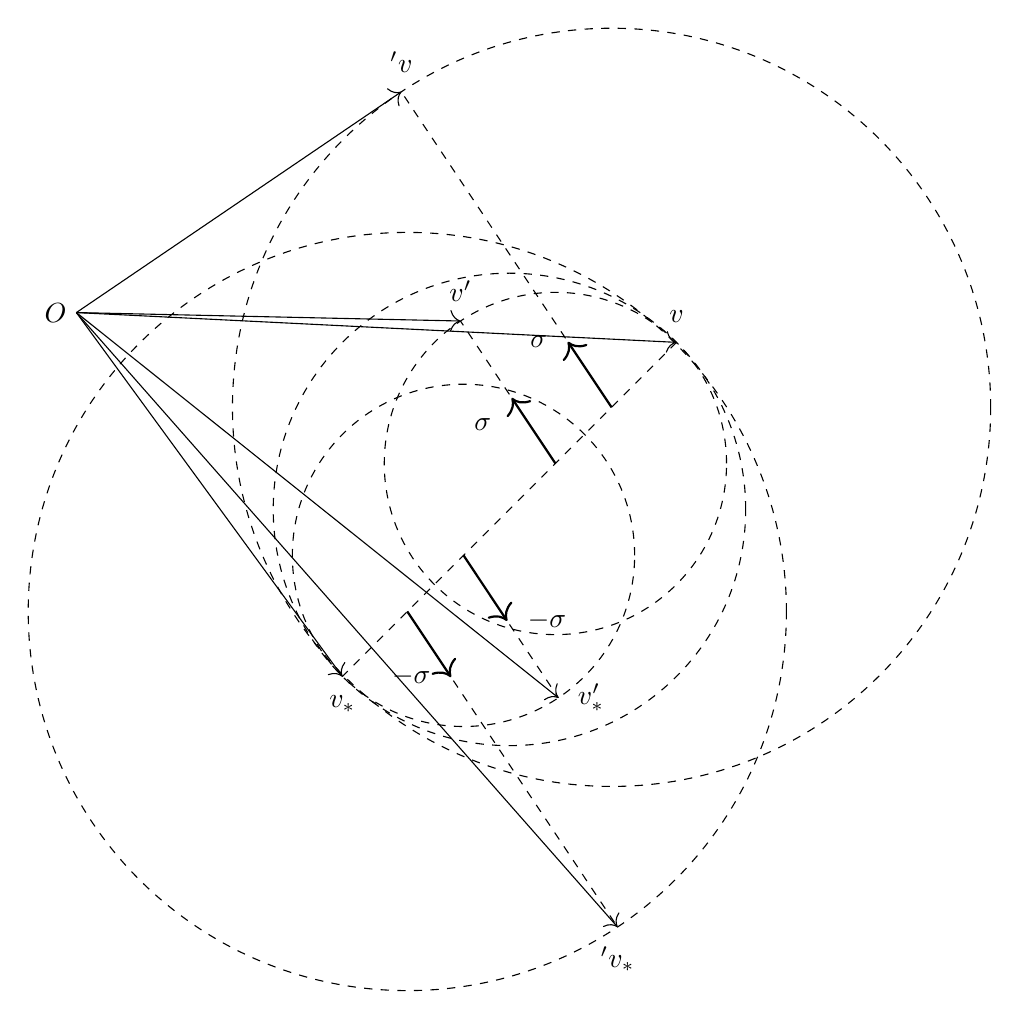
\begin{tikzpicture}
        % long var name to avoid clash
        \newcommand{\graphingParaInelasticParameterERes}{0.45}
        \pgfmathsetmacro{\graphingParaInelasticParameterZ}{(1+\graphingParaInelasticParameterERes)/2}
        \pgfmathsetmacro{\graphingParaInelasticParameterPrimeZ}{(1+1/\graphingParaInelasticParameterERes)/2}
        \coordinate (mid) at (0, 0) {};  % (v + vstar) / 2
        \coordinate [label=left:\( O \)] (orig) at (-5.5, 2.5) {};
        \coordinate (vdir) at (3, 3);
        \coordinate (sigma) at (-3, 4.5);
        \path [name path=lorig] (vdir) -- ($-1*(vdir)$);
        \draw [dashed, name path=circ] (mid) circle [radius=3];
        \path [name intersections={of=lorig and circ, by={v, vStar}}]
            node [label=\( v \)] at (v) {}
            node [label=below:\( v_* \)] at (vStar) {};
        \draw [arrows={->[scale=1.5]}] (orig) -- (v);
        \draw [arrows={->[scale=1.5]}] (orig) -- (vStar);
        \draw [dashed] (v) -- (vStar);
        % post v'
        \coordinate (vPrimeCenter) at ($(v)!\graphingParaInelasticParameterZ!(mid)$);
        \node [draw, dashed, name path=vPrimeCirc] at (vPrimeCenter) [circle through={(v)}] {};
        \path [name path=vPrimeDir] (vPrimeCenter) -- ++(sigma);
        \path [name intersections={of=vPrimeDir and vPrimeCirc, by={vPrime}}]
            node [label=\( v' \)] at (vPrime) {};
        \draw [arrows={->[scale=1.5]}] (orig) -- (vPrime);
        \draw [dashed] (vPrimeCenter) -- (vPrime);
        \draw [thick, arrows={->[scale=1.5]}] (vPrimeCenter) -- ($(vPrimeCenter)!1cm!(vPrime)$)
            node [label=below left:\( \sigma \)] {};
        % post v_*'
        \coordinate (vStarPrimeCenter) at ($(vStar)!\graphingParaInelasticParameterZ!(mid)$);
        \node [draw, dashed, name path=vStarPrimeCirc] at (vStarPrimeCenter) [circle through={(vStar)}] {};
        \path [name path=vStarPrimeDir] (vStarPrimeCenter) -- ++($-1*(sigma)$);
        \path [name intersections={of=vStarPrimeDir and vStarPrimeCirc, by={vStarPrime}}]
            node [label=right:\( v_*' \)] at (vStarPrime) {};
        \draw [arrows={->[scale=1.5]}] (orig) -- (vStarPrime);
        \draw [dashed] (vStarPrimeCenter) -- (vStarPrime);
        \draw [thick, arrows={->[scale=1.5]}] (vStarPrimeCenter) -- ($(vStarPrimeCenter)!1cm!(vStarPrime)$)
            node [label=right:\( -\sigma \)] {};
        % pre {}'v
        \coordinate (primeVCenter) at ($(mid)!\graphingParaInelasticParameterPrimeZ-1!(v)$);
        \node [draw, dashed, name path=primeVCirc] at (primeVCenter) [circle through={($(vStar)!\graphingParaInelasticParameterPrimeZ!(v)$)}] {};
        \path [name path=primeVDir] (primeVCenter) -- ++(sigma);
        \path [name intersections={of=primeVDir and primeVCirc, by={primeV}}]
            node [label=\( {}'v \)] at (primeV) {};
        \draw [arrows={->[scale=1.5]}] (orig) -- (primeV);
        \draw [dashed] (primeVCenter) -- (primeV);
        \draw [thick, arrows={->[scale=1.5]}] (primeVCenter) -- ($(primeVCenter)!1cm!(primeV)$)
            node [label=left:\( \sigma \)] {};
        % pre {}'v_*
        \coordinate (primeVStarCenter) at ($(mid)!\graphingParaInelasticParameterPrimeZ-1!(vStar)$);
        \node [draw, dashed, name path=primeVStarCirc] at (primeVStarCenter) [circle through={($(v)!\graphingParaInelasticParameterPrimeZ!(vStar)$)}] {};
        \path [name path=primeVStarDir] (primeVStarCenter) -- ++($-1*(sigma)$);
        \path [name intersections={of=primeVStarDir and primeVStarCirc, by={primeVStar}}]
            node [label=below:\( {}'v_* \)] at (primeVStar) {};
        \draw [arrows={->[scale=1.5]}] (orig) -- (primeVStar);
        \draw [dashed] (primeVStarCenter) -- (primeVStar);
        \draw [thick, arrows={->[scale=1.5]}] (primeVStarCenter) -- ($(primeVStarCenter)!1cm!(primeVStar)$)
            node [label=left:\( -\sigma \)] {};
%         \draw [dashed] (primeV) -- (primeVStar);
    \end{tikzpicture}
    \caption{Geometrical representation of the post- and pre-collision velocity variables, in the inelastic setting. Note that \( v', v_*', {}'v, {}'v_* \) are collinear.}
\end{figure}

Due to the inelastic nature, we no longer have the reversibility of the particle collision.
More precisely, while the mass and the momentum are still conserved, the energy is not:
\begin{equation*}
    \abs{v'}^2 + \abs{v_*'}^2 - \abs{v}^2 - \abs{v_*}^2
    = -z (1 - z) \abs{v - v_*}^2 \parenth*(1 - \normalized{v - v_*} \cdot \sigma)
    \leq 0
\end{equation*}
which, on a solution \( f \) of the spatially homogeneous inelastic Boltzmann equation, implies
\begin{align*}
    \od{t} \int \abs{v}^2 f
    &= \frac{1}{2} \iiint b(\cos\theta) f f_* \parenth*(\abs{v'}^2 + \abs{v_*'}^2 - \abs{v}^2 - \abs{v_*}^2) \dd{\sigma; v_*; v} \\
    &= -\frac{1}{2} \parenth*(\int b(\cos\theta) (1 - \cos\theta)) \iint f f_* \abs{v - v_*}^2 \\
    &= -\zeta \int \abs{v}^2 f
    \leq 0,
\end{align*}
assuming that the total momentum is zero \( \int v f(t) = 0 \), with natural cooling rate
\begin{equation*}
    \zeta
    \coloneqq z (1 - z) \integration{\sigma}{S^{d - 1}}{}{b(\cos\theta) (1 - \cos\theta)}
    = z (1 - z) (b_0 - b_1)
    \geq 0.
\end{equation*}
% It should be noted that, unlike the elastic case where symmetrization of the kernel is typically done
% \begin{equation*}
%     b_\mathrm{sym}(\cos\theta)
%     \coloneqq \frac{1}{2} (b(\cos\theta) + b(-\cos\theta))
% \end{equation*}
% without losing any information concerning the collision operator, for inelastic collision this will lead to a different interaction for the collisions as, for example, the new kernel will have moment \( b_1 = 0 \) and thus potentially a different natural cooling rate.

As in the case with elastic collision, we can also consider the corresponding Bobylev collision operator
\begin{equation*}
    \widehat{Q}_e(\varphi, \varphi)
    \coloneqq \integration{\sigma}{S^{d - 1}}{}{
        b(\cos\theta) (\varphi^+ \varphi^- - \varphi(0) \varphi)
    }
\end{equation*}
with inelastic post-collision frequencies
\begin{equation} \label{equ:postCollisionFrequencies_inelastic}
\begin{aligned}
    k^+
    &= (1 - \frac{z}{2}) k + \frac{z}{2} \abs{k} \sigma, \\
    k^-
    &= \frac{z}{2} k - \frac{z}{2} \abs{k} \sigma = k - k^+.
\end{aligned}
\end{equation}

\begin{figure}[h]
    \centering
    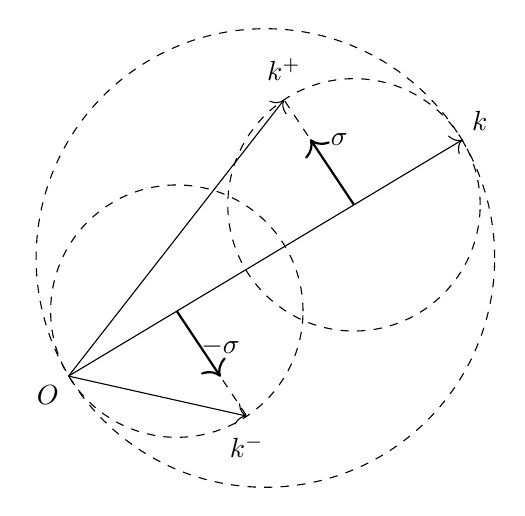
\begin{tikzpicture}
        \coordinate (mid) at (0, 0);
        \coordinate [label=above right:\( k \)] (k) at (2.5, 1.5);
        \coordinate [label=below left:\( O \)] (orig) at ($-1*(k)$);
        \coordinate (offplus) at ($(mid)!0.45!(k)$);
        \coordinate (offminus) at ($(mid)!-0.45!(k)$);
        \coordinate (sigma) at (-1.5, 2.25);
        \node [draw, dashed, circle through={(k)}, name path=circ] at (mid) {};
        \path [draw, arrows={->[scale=1.5]}] (orig) -- (k);
        \path [name path=lplus] (offplus) -- ++(sigma);
        \node [draw, dashed, name path=pluscirc] at (offplus) [circle through={(k)}] {};
        \path [name intersections={of=lplus and pluscirc, by={kplus}}]
            node [label=above:\( k^+ \)] at (kplus) {};
        \draw [dashed] (offplus) -- (kplus);
        \draw [arrows={->[scale=1.5]}] (orig) -- (kplus);
        \draw [thick, arrows={->[scale=1.5]}] (offplus) -- ($(offplus)!1cm!(kplus)$)
            node [label=right:\( \sigma \)] {};
        \path [name path=lminus] (offminus) -- ++($-1*(sigma)$);
        \node [draw, dashed, name path=minuscirc] at (offminus) [circle through={(orig)}] {};
        \path [name intersections={of=lminus and minuscirc, by={kminus}}]
            node [label=below:\( k^- \)] at (kminus) {};
        \draw [dashed] (offminus) -- (kminus);
        \draw [arrows={->[scale=1.5]}] (orig) -- (kminus);
        \draw [thick, arrows={->[scale=1.5]}] (offminus) -- ($(offminus)!1cm!(kminus)$)
            node [label=above:\( -\sigma \)] {};
    \end{tikzpicture}
    \caption{Geometrical representation of the post-collision frequency variables, in the inelastic setting.}
\end{figure}

With such frequency variables, we can define the inelastic kernel constants in the same way as \eqref{def:kernelConstants},
\begin{align*}
    \lambda_p
    &\coloneqq \integration{\sigma}{S^{d - 1}}{}{
        b(\cos\theta) \parenth*(
            1 - \frac{\abs{k^+}^p + \abs{k^-}^p}{\abs{k}^p}
        )
    } \\
    &=\integration{\sigma}{S^{d - 1}}{}{
        b(\cos\theta) \parenth*(
            1 - (1 - z (2 -z) \sin^2\frac{\theta}{2})^{p / 2} - z^p \sin^p\frac{\theta}{2}
        )
    }, \\
    \mu_p
    &\coloneqq \lambda_p / p,
\end{align*}
noting that
\begin{align*}
    \lambda_2
    &= \integration{\sigma}{S^{d - 1}}{}{
            b(\cos\theta)
            \parenth*(1 - (1 - z (2 - z) \sin^2\frac{\theta}{2}) - z^2 \sin^2\frac{\theta}{2}))
        } \\
    &= \integration{\sigma}{S^{d - 1}}{}{b(\cos\theta) 2 z (1 - z) \sin^2\frac{\theta}{2}} \\
    &= \zeta.
\end{align*}


As in the case in the physical space, on a cutoff kernel, the Bobylev collision operator can also be split into gain part and loss part
\begin{equation*}
    \widehat{Q}_e(\varphi, \varphi)
    = \widehat{Q}_e^+(\varphi, \varphi) - \widehat{Q}_e^-(\varphi, \varphi)
\end{equation*}
with the identical definition as the elastic case \eqref{def:bobylevOp_split} on the inelastic frequency variables \eqref{equ:postCollisionFrequencies_inelastic} instead:
\begin{align*}
    \widehat{Q}_e^+(\psi, \varphi)
    &\coloneqq \integration{\sigma}{S^{d - 1}}{}{b(\cos\theta) \varphi^+ \psi^-}, \\
    \widehat{Q}_e^-(\psi, \varphi)
    &\coloneqq b_0 \psi(0) \varphi,
\end{align*}
where, as a property of characteristic functions, \( \psi(0) = 1 \).

Under the shearing effect, the corresponding inelastic analog of the Boltzmann equation \eqref{equ:shearBoltzmann} is then
\begin{equation} \label{equ:shearInelasticBoltzmann}
    \pd{t} f - \divergence[v](A v f) = Q_e(f, f),
\end{equation}
and, taking Fourier transform, the inelastic analog of Bobylev equation \eqref{equ:shearBobylev} is
\begin{equation} \label{equ:shearInelasticBobylev}
    \pd{t} \varphi + A^\transpose k \cdot \grad[k]\varphi
    = \widehat{Q}_e(\varphi, \varphi).
\end{equation}

% We will now justify that the approaches in both \cite{JamesEtAl17SSP} and \cite{BobylevEtAl20SSA} generalize naturally in the setting we are considering.

% \comment{the two extensions do not seem significant enough}

\subsection{Computation in the Physical Space}
% \comment{\protect\citeauthor{JamesEtAl17SSP}, should be about \( 7 \sim 10 \) pages?}

We now argue that the approach in \cite{JamesEtAl17SSP} can be applied naturally to the case with inelastic collision, in the case of cutoff kernel \( b_0 = \int_{S^{d - 1}} b < \infty \).
Using their approach, we will work on the one-point compactification \( \compactRR^d \) of \( \RR^d \) obtained by appending a point of infinity, and consider the nonnegative Radon measures \( f \in \nonnegRadon(\compactRR^d) \) on it.

For our purpose, we will consider two norms on \( \nonnegRadon \), that is the usual \( \lpFunc{1} \) norm \( \measureNorm{f} = \integration[\abs{f}]{v}{\compactRR^d}{}{} \), and the \( s \)-moment norm \( \momentNorm{f}{s} = \integration[\abs{f}]{v}{\compactRR^d}{}{(1 + \abs{v}^s)} \), whenever it is well-defined.

\begin{definition}  % \label{def:shearInelasticBoltzmann_weakSol}
    \( f \in \continuousFunc([0, \infty), \nonnegRadon(\compactRR^d)) \) is a weak solution of \eqref{equ:shearInelasticBoltzmann} on initial condition \( f(t = 0) = f_0 \in \nonnegRadon(\compactRR^d) \) if for every \( T > 0 \) and every test function \( \psi \in \continuousFunc([0, T), \continuousFunc[1](\compactRR^d)) \),
    \begin{equation}  \label{equ:shearInelasticBoltzmann_weakSol}
    \begin{aligned}
        &\alignspacing
        \int_{\RR^d} \psi(T, v) f(T, \dd*{v}) - \int_{\RR^d} \psi(0, v) f_0(\dd*{v}) \\
        &= -\integration{t}{0}{T}{\int_{\RR^d} \pd{t}\psi(t, v) f(t, \dd*{v})}
            - \integration{t}{0}{T}{\int_{\RR^d} (A v \cdot \grad \psi) f(t, \dd*{v})} \\
        &\qquad + \frac{1}{2} \integration{t}{0}{T}{
            \int_{\RR^d} \int_{\RR^d} \int_{S^{d - 1}}
            b(\cos\theta) (\varphi(t, v') + \varphi(t, v_*') - \varphi(t, v) - \varphi(t, v_*)) \dd{\sigma} f(t, \dd*{v_*}) f(t, \dd*{v})
        }.
    \end{aligned}
    \end{equation}
\end{definition}
Note that the above notion of solution is defined via the weak form of the collision operator, and so is a class of weak solution.
A notion of mild solution can also be defined using the strong form of the inelastic collision operator:
\begin{definition}  % \label{def:shearInelasticBoltzmann_mildSol}
    \( f \in \continuousFunc([0, \infty), \nonnegRadon(\compactRR^d)) \) is a mild solution of \eqref{equ:shearInelasticBoltzmann} on initial condition \( f(t = 0) = f_0 \in \nonnegRadon(\compactRR^d) \) if
    \begin{equation}
        f(t, v)
        = S_f(t, 0) f_0 + \integration{s}{0}{t}{S_f(t, s) Q_e^+f(s)}
    \end{equation}
    is satisfied in sense of measure, with \( S_g(t, s) \) defined for each \( g \in \lpFunc{1}([0, T], \nonnegRadon) \) with \( T > 0 \) as
    \begin{equation*}
        S_g(t, s) h_0
        = e^{(t - s) \trace(A)} \exp(-b_0 \integration{\tau}{s}{t}{\measureNorm{g(\tau)}}) h_0(e^{(t - s) A} v)
    \end{equation*}
    on \( 0 \leq s \leq t \leq T \), that is \( h(t) = S_g(t, s) h_s \) solves
    \begin{equation*}
        \pd{t} h - \divergence (A v h)
        = -b_0 h \measureNorm{g(t)}
    \end{equation*}
    on \( [s, T] \) in sense of measure with initial condition \( h(s) = h_s \in \lpFunc{1} \).
\end{definition}

\todo{argue that mild sol is weak sol (how detail should the argument be?)}

The following elementary estimates, analogous to those done in \cite[Thm.~4.2]{JamesEtAl17SSP}, can be derived easily from the definitions:
\begin{lemma}  \label{lem:inelasticOpEstimates}
    If \( f, g \in \nonnegRadon(\compactRR^d) \), then
    \begin{align*}
        \measureNorm{Q_e^+f}
        &= b_0 \measureNorm{f}^2, \\
        \measureNorm{Q_e^+f - Q_e^+g}
        &\leq b_0 (\measureNorm{f} + \measureNorm{g}) \measureNorm{f - g}.
    \end{align*}

    Also, if \( h_1, h_2 \in \lpFunc{1}([0, T], \nonnegRadon) \), then on \( 0 \leq t' \leq t \leq T \),
    \begin{align*}
        \measureNorm{S_{h_1}(t, t') f}
        &= \exp\parenth*(-b_0 \integration{\tau}{t'}{t}{\measureNorm{h_1(\tau)}}) \int f
        \leq \measureNorm{f}, \\
        \measureNorm{S_{h_1}(t, t') f - S_{h_2}(t, t') g}
        &\leq \measureNorm{f - g} + \frac{b_0}{2} (\measureNorm{f} + \measureNorm{g}) \integration{\tau}{t'}{t}{\measureNorm{h_1(\tau) - h_2(\tau)}}.
    \end{align*}

    Similar estimates also hold for \( s \)-moment norm with \( s > 0 \), given that \( \momentNorm{f}{s}, \momentNorm{g}{s} < \infty \), with an additional constant multiplier:
    \begin{align*}
        \momentNorm{Q_e^+f}{s}
        &\lesssim \measureNorm{f} \momentNorm{f}{s}, \\
        \momentNorm{Q_e^+f - Q_e^+g}{s}
        &\lesssim (\momentNorm{f}{s} + \momentNorm{g}{s}) \momentNorm{f - g}{s}, \\
        \momentNorm{S_{h_1}(t, t') f}{s}
        &\lesssim \momentNorm{f}{s}, \\
        \momentNorm{S_{h_1}(t, t') f - S_{h_2}(t, t') g}{s}
        &\lesssim \momentNorm{f - g}{s} + (\momentNorm{f}{s} + \momentNorm{g}{s}) \integration{\tau}{t'}{t}{\measureNorm{h_1(\tau) - h_2(\tau)}}
    \end{align*}
    with constants depending only on \( A, s, T, b_0 \).
\end{lemma}
\begin{proof}
    Noting that \( Q_e^+ f \geq 0 \) by the assumptions and using weak form of the collision operator,
    \begin{align*}
        \measureNorm{Q_e^+}
        &= \integration{v}{\RR^d}{}{
            Q_e(f, f) \cdot 1
        } + \integration{v}{\RR^d}{}{
            Q_e^-(f, f)
        } \\
        &= 0 + \integration{v}{\RR^d}{}{
            \integration{v_*}{\RR^d}{}{
                \integration{\sigma}{S^{d - 1}}{}{
                    b(\cos\theta) f(v) f(v_*)
                }
            }
        } \\
        &= b_0 \measureNorm{f}^2
    \end{align*}
    where the first term vanishes as the constant \( 1 \) is a collision invariant for inelastic collisions.

    Also, with the change of variable for strong form and the collision invariant \( 1 \),
    \begin{align*}
        \measureNorm{Q_e^+f - Q_e^+g}
        &\leq \integration{v}{\RR^d}{}{
            \integration{v_*}{\RR^d}{}{
                \integration{\sigma}{S^{d - 1}}{}{
                    b_e^+(\cos\theta) \abs{{}'f {}'f_* - {}'g {}'g_*}
                }
            }
        } \\
        &= \integration{v}{\RR^d}{}{
            \integration{v_*}{\RR^d}{}{
                \integration{\sigma}{S^{d - 1}}{}{
                    b(\cos\theta) \abs{f f_* - g g_*}
                }
            }
        } \\
        &\leq b_0 \integration{v}{\RR^d}{}{
            \integration{v_*}{\RR^d}{}{
                (\abs{f} \abs{f_* - g_*} + \abs{g_*} \abs{f - g})
            }
        } \\
        &= b_0 (\measureNorm{f} + \measureNorm{g}) \measureNorm{f - g}.
    \end{align*}

    Noting that \( S_{h_1}(t, t') f \geq 0 \) by assumption,
    \begin{align*}
        \measureNorm{S_{h_1}(t, t') f}
        &= \integration{v}{\RR^d}{}{S_{h_1}(t, t') f} \\
        &= \exp\parenth*((t - t') \trace(A) - b_0 \integration{\tau}{t'}{t}{\measureNorm{h_1(\tau)}}) \integration{v}{\RR^d}{}{f(e^{(t - t') A} v)} \\
        &= \exp\parenth*(- b_0 \integration{\tau}{t'}{t}{\measureNorm{h_1(\tau)}}) \integration{v}{\RR^d}{}{f(v)} \\
        &\leq \measureNorm{f}.
    \end{align*}

    As \( \abs{e^{-x} - e^{-y}} \leq \abs{x - y} \) for \( x, y \geq 0 \),
    \begin{align*}
        &\alignspacing
        \measureNorm{S_{h_1}(t, t') f - S_{h_2}(t, t') g} \\
%         &\leq e^{(t - t') \trace(A)} \integration{v}{\RR^d}{}{\abs{
%             e^{-b_0 \integration{\tau}{t'}{t}{\measureNorm{h_1(\tau)}}} f(e^{(t - t') \trace(A)} v)
%             - e^{-b_0 \integration{\tau}{t'}{t}{\measureNorm{h_2(\tau)}}} g(e^{(t - t') \trace(A)} v)
%         }} \\
        &\leq \integration{v}{\RR^d}{}{\abs{
            e^{-b_0 \integration{\tau}{t'}{t}{\measureNorm{h_1(\tau)}}} f(v)
            - e^{-b_0 \integration{\tau}{t'}{t}{\measureNorm{h_2(\tau)}}} g(v)
        }} \\
        &\leq \integration{v}{\RR^d}{}{\parenth*(
            \frac{f + g}{2} \abs{e^{-b_0 \integration{\tau}{t'}{t}{\measureNorm{h_1(\tau)}}} - e^{-b_0 \integration{\tau}{t'}{t}{\measureNorm{h_2(\tau)}}}}
            + \abs{f - g}
        )} \\
        &\leq \frac{b_0}{2} (\measureNorm{f} + \measureNorm{g}) \integration{\tau}{t'}{t}{\measureNorm{h_1(\tau) - h_2(\tau)}} + \measureNorm{f - g}.
    \end{align*}

    On \( s > 0 \), we have
    \begin{equation*}
        \abs{v'}
        \leq \frac{\abs{v} + \abs{v_*}}{2} + \frac{1 - z}{2} (\abs{v} + \abs{v_*}) + \frac{z}{2} (\abs{v} + \abs{v_*})
        = \abs{v} + \abs{v_*},
    \end{equation*}
    so \( \abs{v'}^s \leq (\abs{v} + \abs{v_*})^s \lesssim \abs{v}^s + \abs{v_*}^s \), and similarly \( \abs{v}^s \lesssim \abs{{}'v}^s + \abs{{}'v_*}^s \), which implies
    \begin{align*}
        \momentNorm{Q_e^+f}{s}
        &\lesssim \integration{v}{\RR^d}{}{
            \integration{v_*}{\RR^d}{}{
                \integration{\sigma}{S^{d - 1}}{}{
                    (2 + \abs{{}'v}^s + \abs{{}'v_*}^s) b_e^+(\cos\theta) {}'f {}'f_*
                }
            }
        } \\
        &= \integration{v}{\RR^d}{}{
            \integration{v_*}{\RR^d}{}{
                \integration{\sigma}{S^{d - 1}}{}{
                    (2 + \abs{v}^s + \abs{v_*}^s) b(\cos\theta) f f_*
                }
            }
        } \\
        &\lesssim \measureNorm{f} \momentNorm{f}{s}
    \end{align*}
    and
    \begin{align*}
        &\alignspacing
        \momentNorm{Q_e^+f - Q_e^+g}{s} \\
        &\lesssim \integration{v}{\RR^d}{}{
            \integration{v_*}{\RR^d}{}{
                \integration{\sigma}{S^{d - 1}}{}{
                    (2 + \abs{{}'v}^s + \abs{{}'v_*}^s) b_e^+(\cos\theta) \abs{{}'f {}'f_* - {}'g {}'g_*}
                }
            }
        } \\
        &= \integration{v}{\RR^d}{}{
            \integration{v_*}{\RR^d}{}{
                \integration{\sigma}{S^{d - 1}}{}{
                    (2 + \abs{v}^s + \abs{v_*}^s) b(\cos\theta) \abs{f f_* - g g_*}
                }
            }
        } \\
        &\lesssim \integration{v}{\RR^d}{}{
            \integration{v_*}{\RR^d}{}{
                \integration{\sigma}{S^{d - 1}}{}{
                    (1 + \abs{v}^s)(1 + \abs{v_*}^s) b(\cos\theta)
                    (f \abs{f_* - g_*} + g_* \abs{f - g})
                }
            }
        } \\
        &\lesssim (\momentNorm{f}{s} + \momentNorm{g}{s}) \momentNorm{f - g}{s}.
    \end{align*}

    On \( 0 \leq t' \leq t \leq T \), \( \norm{e^{-(t - t') A}} \) is bounded with constant depending on \( T \). So
    \begin{align*}
        \momentNorm{S_{h_1}(t, t') f}{s}
        &= \integration{v}{\RR^d}{}{
            (1 + \abs{v}^s)
            e^{(t - t') \trace(A)}
            e^{-b_0 \integration{\tau}{t'}{t}{\measureNorm{h_1(\tau)}}}
            f(e^{(t - t') A} v)
        } \\
        &\leq \integration{v}{\RR^d}{}{
            (1 + \norm{e^{-(t - t') A}}^s \abs{v}^s)
            f(v)
        } \\
        &\lesssim \momentNorm{f}{s}
    \end{align*}
    and
    \begin{align*}
        &\alignspacing
        \momentNorm{S_{h_1}(t, t') f - S_{h_2}(t, t') g}{s} \\
        &\leq \integration{v}{\RR^d}{}{
            (1 + \norm{e^{-(t - t') A}}^s \abs{v}^s)
            \parenth*(
                \frac{f + g}{2} \integration{\tau}{t'}{t}{\abs{\measureNorm{h_1(\tau)} - \measureNorm{h_2(\tau)}}}
                + \abs{f - g}
            )
        } \\
        &\lesssim (\momentNorm{f}{s} + \momentNorm{g}{s}) \integration{\tau}{t'}{t}{\measureNorm{h_1(\tau) - h_2(\tau)}}
            + \momentNorm{f - g}{s}.
    \end{align*}
\end{proof}

Given these estimates, the existence of a mild solution of \eqref{equ:shearInelasticBoltzmann} then follows from a standard computation.
\begin{theorem}  \label{thm:shearInelasticBoltz_mildExistence}
    On initial data \( f_0 \in \nonnegRadon \), there exists a unique global-in-time mild solution to \eqref{equ:shearInelasticBoltzmann}.
\end{theorem}
\begin{proof}
    Consider the following subset of the Banach space \( \continuousFunc([0, T], \nonnegRadon) \),
    \begin{equation*}
        X_T
        \coloneqq \setBuilder{f \in \continuousFunc([0, T], \nonnegRadon)}[\norm{f}_{X_T} \coloneqq \sup_{[0, T]} \measureNorm{f(t)} \leq 2 \measureNorm{f_0}]
    \end{equation*}
    with given \( T > 0 \), and the map \( P : X_T \to X_T \) defined as
    \begin{equation*}
        Pf(t, v)
        = S_f(t, 0) f_0 + \integration{s}{0}{t}{S_f(t, s) Q_e^+f(s)}
    \end{equation*}
    in sense of measure.
    It is easy to see that \( X_T \) is closed and thus complete.

    We first show that \( P \) is well-defined when \( T > 0 \) is sufficiently small.
    Let \( f \in X_T \) and \( t \in [0, T] \).
    Then by assumption, \( S_f(t, 0)f_0 \geq 0 \) and \( S_f(t, s) Q_e^+f(s) \geq 0 \) for each \( s \in [0, t] \), so \( Pf(t) \in \nonnegRadon \).
    By \autoref{lem:inelasticOpEstimates},
    \begin{align*}
        \measureNorm{P f(t)}
        &\leq \measureNorm{S_f(t, 0) f_0} + \integration{s}{0}{t}{S_f(t, s) Q_e^+f(s)} \\
%         &\leq \measureNorm{f_0} + \integration{s}{0}{t}{Q_e^+f(s)} \\
        &\leq \measureNorm{f_0} + b_0 \integration{s}{0}{t}{\measureNorm{f(s)}^2} \\
        &\leq \measureNorm{f_0} + b_0 T \norm{f}_{X_T}^2 \\
        &\leq \measureNorm{f_0} (1 + 4 b_0 T \measureNorm{f_0}),
    \end{align*}
    so on \( T \in (0, 1 / (4 b_0 \measureNorm{f_0} + 1)) \) sufficiently small such that \( 1 + 4 b_0 T \measureNorm{f_0} \leq 2 \) and \( \measureNorm{P f(t)} \leq 2 \measureNorm{f_0} \).
    \todo{show \( Pf \) is continuous in time (this is not shown in draft\_v3)}
    This implies \( Pf \in X_T \).

    Let \( f, g \in X_T \) with such \( T \).
    Then for \( t \in [0, T] \),
    \begin{align*}
        &\alignspacing
        \measureNorm{Pf(t) - Pg(t)} \\
        &\leq \measureNorm{S_f(t, 0) f_0 - S_g(t, 0) f_0}
            + \integration{s}{0}{t}{\measureNorm{S_f(t, s) Q_e^+ f(s) - S_g(t, s) Q_e^+g(s)}} \\
        &\leq b_0 \measureNorm{f_0} \integration{\tau}{0}{t}{\measureNorm{f(\tau) - g(\tau)}} \\
            &\qquad + \integration{s}{0}{t}{\parenth*(
                \measureNorm{Q_e^+f(s) - Q_e^+g(s)}
                + \frac{b_0}{2} (\measureNorm{Q_e^+f(s)} + \measureNorm{Q_e^+g(s)}) \integration{\tau}{s}{t}{\measureNorm{f(\tau) - g(\tau)}}
            )} \\
%         &\leq b_0 \measureNorm{f_0} \integration{\tau}{0}{t}{\measureNorm{f(\tau) - g(\tau)}} \\
%             &\qquad + \integration{s}{0}{t}{\parenth*(
%                 b_0 (\measureNorm{f(s)} + \measureNorm{g(s)}) \measureNorm{f(s) - g(s)}
%                 + \frac{b_0}{2} b_0 (\measureNorm{f(s)}^2 + \measureNorm{g(s)}^2) \integration{\tau}{s}{t}{\measureNorm{f(\tau) - g(\tau)}}
%             )} \\
        &\leq b_0 \measureNorm{f_0} T \norm{f - g}_{X_T}
            + T \parenth*(
                4 b_0 \measureNorm{f_0} \norm{f - g}_{X_T}
                + 4 b_0^2 \measureNorm{f_0}^2 T \norm{f - g}_{X_T}
            ) \\
        &= (5 b_0 T \measureNorm{f_0} + 4 b_0^2 T^2 \measureNorm{f_0}^2) \norm{f - g}_{X_T},
    \end{align*}
    so, on \( T \in (0, \frac{1}{20 b_0 \measureNorm{f_0} + 1}) \) sufficiently small such that
    \begin{equation*}
        5 (b_0 T \measureNorm{f_0}) + 4 (b_0 T \measureNorm{f_0})^2
        \leq 1 / 2,
    \end{equation*}
    \( P \) is a contraction on \( X_T \).

    For such horizon \( T \), by Banach contraction theorem, there exists a unique \( f \in X_T \) such that \( f = Pf \).
    By the definition, \( f \) is a mild solution on \( [0, T] \) with initial data \( f_0 \).
    Applying the operator \( \pd{t} - \divergence(A v \;\text{--}) \) and integrating with test function \( \psi = 1 \) yields
%     \todo{This is a bit vague. Need to be more detailed}
    \begin{equation*}
        \measureNorm{f(T)} - \measureNorm{f_0}
        = \integration{s}{0}{T}{\integration{v}{\RR^d}{}{\pd{t} f}}
        = -\integration{s}{0}{T}{\integration{v}{\RR^d}{}{A v f \cdot \grad 1}}
            + \integration{s}{0}{T}{\integration{v}{\RR^d}{}{Q_e f}}
        = 0,
    \end{equation*}
    which implies \( \measureNorm{f(T)} = \measureNorm{f_0} \).
    As the selection of \( T \) depends only on \( b_0 \) and \( \measureNorm{f_0} \), we may extend the solution to \( [T, 2 T] \) using \( f(T) \) as the initial data.
    Iterating this process yields a unique global-in-time mild solution.
\end{proof}

We also have the following estimates concerning the moments of such mild solutions.
\begin{theorem}  \label{thm:shearInelasticBoltz_momentBoundednessAndApprox}
    Let \( f \in \continuousFunc([0, \infty), \nonnegRadon) \) be the mild solution from \autoref{thm:shearInelasticBoltz_mildExistence} on initial \( f_0 \in \nonnegRadon \) with finite \( s_0 \)-moment for some \( s_0 > 1 \), that is, \( \int \abs{v}^{s_0} f_0 < \infty \).
    Then the \( s_0 \)-moments of \( f \) is locally bounded, that is, for each \( T \in (0, \infty) \), \( \sup_{[0, T]} \int \abs{v}^{s_0} f(t) < \infty \).

    Moreover, the weak solution formulation \eqref{equ:boltzmannCollisionOp_inelastic_weakForm} is satisfied for all \( \psi \in \continuousFunc([0, T], \continuousFunc[1](\RR^d)) \) with \( \abs{\psi} + \abs{v} \abs{\grad \psi} \lesssim 1 + \abs{v}^{s'} \) uniformly on \( [0, T] \) for some \( s' \in (1, s_0) \).

    Furthermore, for each \( s > s_0 \) and \( T \in (0, \infty) \), there exists an approximation sequence \( f_n \in \continuousFunc([0, T], \nonnegRadon) \) with \( \sup_{[0, T]} \int \abs{v}^s f_n(t) < \infty \) such that \( \sup_{[0, T]} \momentNorm{f_n(t) - f(t)}{s_0} \to 0 \).
\end{theorem}

Note that if \( \psi \in \continuousFunc(\compactRR^d) \), the limit \( \limit*{v}[\infty] \psi(v) \) must exist and be finite, while for \( \psi \in \continuousFunc(\RR^d) \) there is no such constraint.
In particular, this theorem indicates that, for the weak formulation, we can use an unbounded test function, given that there is still an appropriate control on its growth.

\begin{proof}
    For \( t \in [0, T] \), as mass is conserved, we have
    \begin{align*}
        \momentNorm{f(t)}{s_0}
        &\leq \momentNorm{S_f(t, 0) f_0}{s_0} + \integration{\tau}{0}{t}{\momentNorm{S_f(t, \tau) Q_e^+f(\tau)}{s_0}} \\
        &\lesssim \momentNorm{f_0}{s_0} + \integration{\tau}{0}{t}{\measureNorm{f(\tau)} \momentNorm{f(\tau)}{s_0}} \\
        &= \momentNorm{f_0}{s_0} + \measureNorm{f_0} \integration{\tau}{0}{t}{\momentNorm{f(\tau)}{s_0}},
    \end{align*}
    so Gr\"onwall inequality implies \( \momentNorm{f(t)}{s_0} \lesssim \momentNorm{f_0}{s_0} < \infty \), with constant depending on \( T \).

    Let \( \psi \in \continuousFunc([0, T], \continuousFunc[1](\RR^d)) \) with \( \abs{\psi} + \abs{v} \abs{\grad \psi} \lesssim 1 + \abs{v}^{s'} \) with \( s' \in (1, s_0) \).
    Then there exists a sequence of cutoff approximations \( \psi_n \in \continuousFunc([0, T], \continuousFunc[1](\compactRR^d)) \) for which \( \psi_n, \grad \psi_n \) converges pointwise to \( \psi, \grad \psi \), and \( \abs{\grad \psi_n} \lesssim 1 + \abs{\grad \psi} \).
    The weak formulation on \( \psi_n \) then implies
    \begin{align*}
        &\alignspacing
        \int \psi_n(T) f(T) - \int \psi_n(0) f_0 + \integral{0}{T} \int f(t) \pd{t} \psi_n + \integral{0}{T} \int A v f(t) \cdot \grad \psi_n \\
        &= \frac{1}{2} \integral{0}{T} \iiint b(\cos\theta) f(t) f_*(t) \parenth*(
            \psi_n'(t) + {\psi_n}_*'(t) - \psi_n(t) - {\psi_n}_*(t)
        ).
    \end{align*}
    By assumption on \( \psi \), there exists a neighbourhood \( B(0, R) \) of the origin on which \( \abs{\grad \psi} \lesssim 1 \) uniformly on \( [0, T] \), and on \( \abs{v} \geq R \) we have \( \abs{\grad \psi} \lesssim (1 + \abs{v}^{s'}) / \abs{v} \lesssim 1 + \abs{v}^{s' - 1} \).
    Then at time \( t \in [0, T] \), the \( \sigma \)-integration can be estimated as
    \begin{align*}
        &\alignspacing
        \abs{\integration{\sigma}{S^{d - 1}}{}{b(\cos\theta) (\psi_n' + {\psi_n}_*' - \psi_n - {\psi_n}_*)}} \\
        &\lesssim \sup_\sigma \abs{
            (v' - v) \cdot \integration{\lambda}{0}{1}{\parenth*(
                \grad \psi_n(v + \lambda (v' - v))
                - \grad \psi_n(v_* + \lambda (v_*' - v_*))
            )}
        } \\
        &\lesssim \abs{v - v_*} \sup_{\abs{u - v} \leq z \abs{v - v_*}} \abs{\grad \psi_n(u)}
            + \abs{v - v_*} \sup_{\abs{u - v_*} \leq z \abs{v - v_*}} \abs{\grad \psi_n(u)} \\
        &\lesssim (\abs{v} + \abs{v_*}) \sup_{\abs{u} \leq (1 + z) (\abs{v} + \abs{v_*})} \abs{\grad \psi_n(u)} \\
        &\lesssim (\abs{v} + \abs{v_*}) \parenth*(1 + \sup_{\abs{u} \leq (1 + z) (\abs{v} + \abs{v_*})} \abs{\grad \psi(u)}) \\
        &\lesssim (\abs{v} + \abs{v_*}) \parenth*(1 + (\abs{v} + \abs{v_*})^{s' - 1}) \\
        &\lesssim 1 + \abs{v}^{s'} + \abs{v}^{s'}
    \end{align*}
    with constant independent of \( n \) and \( t \), noting that \( \abs{v' - v} = \abs{v_*'- v_*} \leq z \abs{v - v_*} \sim \abs{v - v_*} \), and thus \( v + \lambda (v' - v) \in B(v, z \abs{v - v_*}) \), \( v_* + \lambda (v_*' - v_*) \in B(v_*, z \abs{v - v_*}) \) for each \( \lambda \in [0, 1] \).
    \highlight[comment={Detailed proof?}]{With dominated convergence theorem, by passing \( n \to \infty \), this implies the weak formulation \eqref{equ:shearInelasticBoltzmann_weakSol} holds for \( \psi \).}

    We now construct a sequence \( f_n \) that approximates \( f \) and has finite \( s \)-moment.
    For each \( n \), let \( f_n \in \continuousFunc([0, \infty), \nonnegRadon) \) be the mild solution from \autoref{thm:shearInelasticBoltz_mildExistence} on cutoff initial data \( f_{n0} = f_0 \indicator[\abs{v} \leq n] \).

    By previous argument,
    \begin{align*}
        \sup_{[0, T]} \momentNorm{f_n(t)}{s}
        &\lesssim \momentNorm{f_{n0}}{s}
        < \infty, \\
        \sup_{[0, T]} \momentNorm{f_n(t)}{s_0}
        &\lesssim \momentNorm{f_{n0}}{s_0}
        \leq \momentNorm{f_0}{s_0}
        < \infty.
    \end{align*}
    Since \( \int (1 + \abs{v}^{s_0}) f_0 = \momentNorm{f_0}{s_0} < \infty \), we also have
    \begin{equation*}
     \momentNorm{f_{n0} - f_0}{s_0}
     = \int (1 + \abs{v}^{s_0}) f_0 \indicator[\abs{v} > n]
     \xrightarrow{n \to \infty} 0.
    \end{equation*}

    Furthermore, on \( 0 \leq t \leq T < \infty \), noting that \( \measureNorm{f} \leq \momentNorm{f}{s_0} \) for all \( f \),
    \begin{align*}
        &\alignspacing
        \momentNorm{f_n(t) - f(t)}{s_0} \\
        &\leq \momentNorm{S_{f_n}(t, 0) f_{n0} - S_f(t, 0) f_0}{s_0}
            + \integration{\tau}{0}{t}{
                \momentNorm{S_{f_n}(t, \tau) Q_e^+f_n(\tau) - S_f(t, \tau) Q_e^+f(\tau)}{s_0}
            } \\
%         &\lesssim \momentNorm{f_{n0} - f_0}{s_0}
%             + (\momentNorm{f_{n0}}{s_0} + \momentNorm{f_0}{s_0}) \integration{\tau}{0}{t}{\measureNorm{f_n(\tau) - f(\tau)}} \\
%             &\qquad + \integration{\tau}{0}{t}{
%                 \momentNorm{Q_e^+f_n(\tau) - Q_e^+f(\tau)}{s_0}
%             } \\
%             &\qquad + \integration{\tau}{0}{t}{
%                 (\momentNorm{Q_e^+f_n(\tau)}{s_0} + \momentNorm{Q_e^+f(\tau)}{s_0}) \integration{\tau'}{\tau}{t}{\measureNorm{f_n(\tau') - f(\tau')}}
%             } \\
        &\lesssim \momentNorm{f_{n0} - f_0}{s_0}
            + \momentNorm{f_0}{s_0} \integration{\tau}{0}{t}{\measureNorm{f_n(\tau) - f(\tau)}} \\
            &\qquad + \integration{\tau}{0}{t}{
                    (\momentNorm{f_n(\tau)}{s_0} + \momentNorm{f(\tau)}{s_0}) \momentNorm{f_n(\tau) - f(\tau)}{s_0}
            } \\
            &\qquad + \integration{\tau}{0}{t}{
                (\momentNorm{f_n(\tau)}{s_0}^2 + \momentNorm{f(\tau)}{s_0}^2)
                \integration{\tau'}{\tau}{t}{
                    \measureNorm{f_n(\tau') - f(\tau')}
                }
            } \\
        &\lesssim \momentNorm{f_{n0} - f_0}{s_0}
            + (\momentNorm{f_0}{s_0} + \momentNorm{f_0}{s_0}^2 T ) \integration{\tau}{0}{t}{\momentNorm{f_n(\tau) - f(\tau)}{s_0}},
    \end{align*}
    so by Gr\"onwall inequality, \( \momentNorm{f_n(t) - f(t)}{s_0} \lesssim \momentNorm{f_{n_0} - f_0}{s_0} \) on \( [0, T] \) with constant independent of \( n \) and \( t \), which yields the convergence.
\end{proof}

\subsubsection{Stationary Self-Similar Radon Profile}

In \cite{JamesEtAl17SSP} it is shown that there exists a stationary self-similar profile \( f \in \nonnegRadon \), that is, on self-similar parameter \( \beta \in \RR \),
\begin{equation}  \label{equ:shearBoltzmann_selfSim}
    \pd{t} f - \divergence[v] (A_\beta v f) = Q(f, f)
\end{equation}
% \todo{move this to intro}
with notation \( A_\beta = A + \beta I \), under the assumption that the shearing is small, or quantitatively \( \norm{A} \ll 1 \).
Here, we will show that the same conclusion holds, with the additional assumption that the collision is also not too different from elastic collision, or quantitatively \( 1 - z \ll 1 \), on the corresponding inelastic equation
\begin{equation}  \label{equ:shearInelasticBoltzmann_selfSim}
    \pd{t} f - \divergence[v] (A_\beta v f) = Q_e(f, f).
\end{equation}

As argued in \cite{JamesEtAl17SSP} for the elastic case, the existence of such finite energy profile depends critically on the evolution of the second moment tensor \( B(t) \coloneqq \int \tensorPower{v} f(t) \) of the solution.
Formally, with \( \hat{u} = \normalized{v - v_*} \),
\begin{align*}
    \od{t} B
    &= \pd{t} \int \tensorPower{v} f \\
    &= -\int \tensorPower{v} \divergence (A v f) + \int \tensorPower{v} Q_e(f, f) \\
    &= -\int A v f \cdot \grad (\tensorPower{v})
        + \frac{1}{2} \iiint b(\sigma \cdot \hat{u}) f f_* (\tensorPower{v'} + \tensorPower{v_*'} - \tensorPower{v} - \tensorPower{v_*}) \\
    &= -\int (v \otimes (A v) + (A v) \otimes v) f \\
        &\qquad - \frac{1}{4} \iiint b(\sigma \cdot \hat{u}) f f_* \abs{v - v_*} (z (2 - z) \tensorPower{\hat{u}} - z^2 \tensorPower{\sigma} - z (1 - z) (\hat{u} \otimes \sigma + \sigma \otimes \hat{u})) \\
    &= -(\int \tensorPower{v} A^\transpose f + \int A \tensorPower{v} f) \\
        &\qquad - \frac{1}{4} \iint f f_* \abs{v - v_*}^2 ((2 \zeta + z^2 d c_{11}) \tensorPower{\hat{u}} - z^2 c_{11} I) \\
    &= -\parenth*(A B + B A^\transpose + \zeta B + z^2 \frac{d c_{11}}{2} (B - \frac{\trace(B)}{d} I)),
\end{align*}
noting that
\begin{equation*}
    \integration{\sigma}{S^{d - 1}}{}{b(\sigma \cdot \hat{u}) \tensorPower{\sigma}}
    = (b_0 - d c_{11}) \tensorPower{\hat{u}} + c_{11} I
\end{equation*}
for all \( \hat{u} \in S^{d - 1} \), with constant
\begin{equation*}
    c_{11}
    \coloneqq \frac{b_0 - b_2}{d - 1}
    = \frac{1}{d - 1} \integration{\sigma}{S^{d - 1}}{}{b(\cos\theta) \sin^2\theta}.
\end{equation*}
This yields the evolution equation for the second moment tensor,
\begin{equation}  \label{equ:inelastic_2ndMomentEvolution}
    \od{t} B + A B + B A^\transpose + \zeta B + z^2 \frac{d c_{11}}{2} (B - \frac{\trace(B)}{d} I) = 0,
\end{equation}
and, in the case where self-similar scaling with parameter \( \beta \in \RR \) is present,
\begin{align*}
    \od{t} B + A_\beta B + B A_\beta^\transpose + \zeta B + z^2 \frac{d c_{11}}{2} (B - \frac{\trace(B)}{d} I)
    &= 0, \\
    \text{that is} \quad
    \od{t} B + A B + B A^\transpose + (\zeta + 2 \beta) B + z^2 \frac{d c_{11}}{2} (B - \frac{\trace(B)}{d} I)
    &= 0,
\end{align*}
which, in the view of the second moment tensor, indicates that self-similar force \( -\beta \divergence(v f) \) introduced from the scaling and inelastic damping are equivalent.

\begin{theorem}  \label{thm:shearInelasticBoltz_finiteEnergyProfile}
    There exists \( \epsilon > 0 \) such that the following holds:
    if \( \norm{A} < \epsilon \) and \( 1 - z < \epsilon \), then there exists self-similar parameter \( \beta \in \RR \) such that for all \( \Theta > 0 \), there exists a stationary self-similar profile \( f \in \nonnegRadon \) that solves \eqref{equ:shearBoltzmann_selfSim} in sense of measure and satisfies \( \int (1, v, \abs{v}^2) f = (1, 0, \Theta) \).
\end{theorem}
\begin{proof}
    The argument is mostly an adaption of \cite[Lem.~4.19]{JamesEtAl17SSP} in the inelastic setting.

    Consider first the linear map \( L(B) = -(A B + B A^\transpose + \zeta B + z^2 \frac{d c_{11}}{2} (B - \frac{\trace(B)}{d} I)) \).
    On \( A = 0 \), the map \( L(B) = -\zeta B - z^2 \frac{d c_{11}}{2} (B - \frac{\trace(B)}{d} I) \), which it is easy to note that the eigenvalues are \( -\zeta \in \RR \), which is a simple eigenvalue and is associated to the eigenspace \( \setBuilder{c I}[c \in \CC] \), and \( - \zeta - z^2 \frac{d c_{11}}{2} < -\zeta \), associated to the eigenspace \( \setBuilder{B \in \CC^{d \times d}}[\trace(B) = 0] \).

    By perturbation \cite{Kato95PTL} (also \cite[Lem.~4.16]{JamesEtAl17SSP}), for each \( z \in (1 / 2, 1] \), there exists \( \epsilon > 0 \) such on \( \norm{A} < \epsilon \), \( L \) has a real eigenvalue \( 2 \beta \in \RR \) which is simple, has the largest real part among all eigenvalues, satisfies the control
    \begin{equation*}
        \abs{2 \beta + \zeta}
        \leq C_L \norm{A}
    \end{equation*}
    with some constant \( C_L > 0 \) independent of \( A \) (but may depend on \( z \)), and there exists an associated positive semidefinite eigenvector \( B \in \RR^{d \times d} \) with \( \trace(B) = 1 \), with the spectral gap \( \nu > 0 \) of \( L \) such that for every solution \( C(t) \) of \eqref{equ:inelastic_2ndMomentEvolution} on self-similar parameter \( \beta \), there exists \( \lambda \in \RR \) such that
    \begin{equation*}
        \norm{C(t) - \lambda^2 B}
        \lesssim e^{-\nu t}.
    \end{equation*}
    Since on \( A = 0 \) the spectral gap is \( \nu = z^2 \frac{d c_{11}}{2} > 0 \), on \( \norm{A}, 1 - z \) sufficiently small, by perturbation, we still have \( \nu \gtrsim 1 \).

    We will take such \( \beta \) as the self-similar parameter, in which case \( B \) is a positive semidefinite stationary solution of \eqref{equ:inelastic_2ndMomentEvolution}.

    Let \( s \in (2, 4] \) be fixed. Then on \( C_* > 0 \) sufficiently large,
    \begin{equation*}
        K
        \coloneqq \setBuilder{G \in \nonnegRadon}[\int (1, v, \tensorPower{v}) G = (1, 0, \Theta B),\, \int \abs{v}^s G \leq C_*]
    \end{equation*}
    is nonempty, bounded in \( \nonnegRadon \), convex, and weak-* closed, so weak-* compact.

    \todo{\( K \) weak-* compact? draft\_v3 kind of omitted it. Suff to show weakly closed}
    \todo{but don't we need weakly compact instead of weak-* compact? James did weak-*}
    Let \( S : [0, \infty] \times \nonnegRadon \to \nonnegRadon \) be the mild solution operator such that \( G(t) = S(t) G_0 \) is the mild solution constructed from \autoref{thm:shearInelasticBoltz_mildExistence} on initial data \( G_0 \in \nonnegRadon \), and \( S(t) \) forms a semigroup.
    By the conservation of mass and momentum, and due to the definition of \( B \), we have \( \int (1, v, \tensorPower{v}) S(t)G = (1, 0, \Theta B) \) for all \( G \in K \).

    We first show that on each fixed \( T > 0 \), \( S \) is uniformly weakly continuous on \( [0, T] \times K \).
    Let \( 0 \leq t_1 \leq t_2 \leq T \) and \( G_0 \in \nonnegRadon \) with \( \int \abs{v}^s G_0 < \infty \).
    By \autoref{thm:shearInelasticBoltz_momentBoundednessAndApprox}, \( G(t) = S(t) G_0 \) has finite \( s \)-moment on \( [0, T] \).
    Let \( \varphi \in \continuousFunc[2](\compactRR^d) \) with \( \abs{v} \abs{\grad \varphi} + \abs{v}^2 \abs{\grad^2 \varphi} \lesssim 1 + \abs{v}^s \).
    Then expanding to the second order,
    \begin{align*}
        &\alignspacing
        \abs{\varphi' + \varphi_*' - \varphi - \varphi_*} \\
        &\leq \abs{v' - v} \abs{\grad \varphi - \grad \varphi_*}
            + \abs{v' - v}^2 \integral{0}{1} (\abs{\grad^2 \varphi(v + \lambda (v' - v))} + \abs{\grad^2 \varphi(v_* + \lambda (v_*' - v_*))}) \\
        &\lesssim \abs{v - v}^2 \sup_{} \abs{\grad^2 \varphi},
    \end{align*}
    as \( \abs{v' - v} = \abs{v_*' - v_*} = z \abs{v - v_*} \sin\frac{\theta}{2} \leq \abs{v - v_*} \),
    and so by weak formulation we have
    \begin{align*}
        &\alignspacing
        \abs{\int \varphi G(t_1) - \int \varphi G(t_2)} \\
        &\leq \integral{t_1}{t_2} \int \abs{A v \cdot \grad \varphi_n} G(t)
            + \frac{1}{2} \integral{t_1}{t_2}
                \iiint b(\cos\theta) G(t) G_*(t) \abs{\varphi' + \varphi_*' - \varphi - \varphi*}
            \\
        &\lesssim \integral{t_1}{t_2} \int \abs{v} \abs{\grad \varphi} G(t)
            + \integral{t_1}{t_2} \iiint b(\cos\theta) G(t) G_*(t) \abs{v - v_*}^2 \abs{\grad^2 \varphi} \\
        &\leq \integral{t_1}{t_2} (
            \int (1 + \abs{v}^s) G(t)
            + \iint G(t) G_*(t) (1 + \abs{v}^s + \abs{v_*}^s)
        ) \\
        &\lesssim \abs{t_1 - t_2} (1 + \sup_{[t_1, t_2]} \momentNorm{G(t)}{s})^2 \\
        &\lesssim \abs{t_1 - t_2} (1 + C_*)^2.
    \end{align*}
    \highlight[comment={Do we have a detailed proof on this one?}]{By a standard density argument}, this also holds for test function in \( \continuousFunc(\compactRR^d) \).
    This implies that \( S \) is weakly continuous uniformly on \( [0, T] \).

    Let \( T > 0 \) be fixed.
    To show the weak continuity of \( S(T) \) on \( K \), it suffices to show the continuity in the \( 1 \)-Wasserstein metric \( W \) on \( \nonnegRadon \),
    \begin{equation*}
        W(f, g)
        \coloneqq \sup_{\lipConst(\varphi) \leq 1} \int (f - g) \varphi
    \end{equation*}
    where \( \lipConst(\varphi) \coloneqq \sup_{x \neq y} \abs{\varphi(x) - \varphi(y)} / \abs{x - y} \) is the Lipschitz constant of function \( \varphi \).

    Let \( f_0, g_0 \in K \), and \( \varphi \in \continuousFunc(\compactRR^d) \) with \( \lipConst(\varphi) \leq 1 \).
    Fix \( t \in [0, T] \) and \( \psi(s, v) = \varphi(e^{(t - s) A} v) \) for \( s \in [0, t] \).
    Then \( \psi \) satisfies \( \pd{s} \psi + A v \cdot \grad \psi = 0 \) in sense of measure, and thus by weak formulation on \( \psi \),
    \begin{align*}
        &\alignspacing
        \int \varphi (f(t) - g(t)) \\
        &= \int \varphi(e^{t A} v) (f_0 - g_0) \dd{v} \\
            &\qquad + \frac{1}{2} \integral{0}{t} \iiint b(\cos\theta) f(s) (\psi'(s) + \psi_*'(s) - \psi(s) - \psi_*(s)) (f_*(s) - g_*(s)) \dd{\sigma; v_*; v; s} \\
            &\qquad + \frac{1}{2} \integral{0}{t} \iiint b(\cos\theta) g_*(s) (\psi'(s) + \psi_*'(s) - \psi(s) - \psi_*(s)) (f(s) - g(s)) \dd{\sigma; v_*; v; s}.
    \end{align*}

    Since \( \lipConst(\varphi) \leq 1 \), we have \( \lipConst(\psi(s)) \leq \lipConst(\varphi) \norm{e^{(t - s)} A} \leq \sup_{[0, T]} \norm{e^{s A}} \).
    So,
    \begin{equation*}
        \int \varphi(e^{t A} v) (f_0 - g_0)
        = (\sup_{[0, T]} \norm{e^{s A}}) \int \frac{\varphi(e^{t A} v)}{\sup_{[0, T]} \norm{e^{s A}}} (f_0 - g_0)
        \lesssim W(f_0, g_0),
    \end{equation*}
    with constant depending only on \( T \).

    Let \( \hat{e} \in S^{d - 1} \) be a fixed unit vector, and \( R = R(v, v_*) \) be a rotation such that \( R^\transpose \normalized{v - v_*} = \hat{e} \).
    Then
    \begin{equation*}
        \iint b\parenth*(\normalized{v - v_*} \cdot \sigma) f(s) \psi'(s) \dd{\sigma; v}
%         &= \iint b(\normalized{v - v_*} \cdot \sigma) f(s, v) \psi(s, \frac{v + v_*}{2} + \frac{1 - z}{2} (v - v_*) + \frac{z}{2} \abs{v - v_*} \sigma) \dd{\sigma; v} \\
        = \iint b(\hat{e} \cdot \sigma) f(s, v) \psi(s, \tilde{v}') \dd{\sigma; v}
    \end{equation*}
    with \( \tilde{v}'(v, v_*, \sigma) = \frac{v + v_*}{2} + \frac{1 - z}{2} (v - v_*) + \frac{z}{2} \abs{v - v_*} R(v, v_*) \sigma \).
    Since
    \begin{equation*}
        \norm{\grad[v_*] (\abs{v - v_*} R(v, v_*) \sigma)}
        \lesssim \norm{(R(v, v_*) \sigma) \otimes \normalized{v - v_*}} + \abs{v - v_*} \norm{\grad[v_*] \normalized{v - v_*}}
        \lesssim 1
    \end{equation*}
    uniformly in \( v_* \), so
    \begin{equation*}
        \lipConst_{v_*}(\tilde{v}')
        \leq \frac{1}{2} + \frac{1 - z}{2} + \frac{z}{2} \sup_{v_*} \norm{\grad[v_*] (\abs{v - v_*} R(v, v_*) \sigma)}
        \lesssim 1,
    \end{equation*}
    which implies
    \begin{equation*}
        \lipConst_{v_*}\parenth*(\iint b(\normalized{v - v_*} \cdot \sigma) f(s) \psi'(s) \dd{\sigma; v})
        \leq \iint b(\hat{e} \cdot \sigma) f(s) \lipConst(\psi(s)) \lipConst_{v_*}(\tilde{v}')
        \lesssim 1
    \end{equation*}
    with constant depending on \( T \).
    Similarly, \( \lipConst_{v_*}(\iint b(\normalized{v - v_*} \cdot \sigma) f(s) \psi_*'(s) \dd{\sigma; v}) \lesssim 1 \).
    Furthermore,
    \begin{equation*}
        \lipConst_{v_*}\parenth*(-\iint b(\cos\theta) f(s) \psi(s) \dd{\sigma; v})
        = 0,
    \end{equation*}
    \begin{equation*}
        \lipConst_{v_*}\parenth*(-\iint b(\cos\theta) f(s) \psi_*(s) \dd{\sigma; v})
        = \lipConst_{v_*}\parenth*(-\psi_*(s) \iint b(\cos\theta) f(s) \dd{\sigma; v})
        \sim \lipConst(\psi)
        \lesssim 1.
    \end{equation*}
    Combined,
    \begin{equation*}
        \lipConst_{v_*}\parenth*(\iint b(\cos\theta) f(s) (\psi'(s) + \psi_*'(s) - \psi(s) - \psi_*(s)) \dd{\sigma; v})
        \lesssim 1
    \end{equation*}
    which implies
    \begin{equation*}
         \iiint b(\cos\theta) f(s) (\psi'(s) + \psi_*'(s) - \psi(s) - \psi_*(s)) (f_*(s) - g_*(s)) \dd{\sigma; v_*; v}
         \lesssim W(f(s), g(s))
    \end{equation*}
    with constant depending only on \( T \).
    With a similar computation, we also have
    \begin{equation*}
         \iiint b(\cos\theta) g_*(s) (\psi'(s) + \psi_*'(s) - \psi(s) - \psi_*(s)) (f(s) - g(s)) \dd{\sigma; v_*; v}
         \lesssim W(f(s), g(s)).
    \end{equation*}
    Thus, on \( t \in [0, T] \),
    \begin{equation*}
        W(f(t), g(t)) \lesssim W(f_0, g_0) + \integral{0}{t} W(f(s), g(s))
    \end{equation*}
    with constant independent of \( t \), and thus Gr\"onwall inequality implies that \( W(f(t), g(t)) \lesssim W(f_0, g_0) \) with constant depending only on \( T \).
    Hence, \( S(t) \) is weakly continuous on \( K \) for each fixed \( t \).

    It remains to show that \( S(t) K \subseteq K \) if \( C_* \) is sufficiently large.
    By the selection of \( \beta \), it suffices to show that \( \int \abs{v}^s S(t)f_0 \leq C_* \) on \( f_0 \in K \).
    Let \( f_{n0} = f_0 \indicator[\abs{v} \leq n] \) and \( f_n(t) = S(t) f_{n0} \).
    As constructed in \autoref{thm:shearInelasticBoltz_momentBoundednessAndApprox}, \( \momentNorm{f_n(t) - f(t)}{2} \to 0 \), so on \( n \) sufficiently large we have \( \momentNorm{f_n(t)}{2} \lesssim \momentNorm{f(t)}{2} \), with a constant independent of \( n \).
    By \cite[Lem.~3.3]{GambaEtAl04BED}, we have the following Povzner inequality for inelastic variables on \( s > 2 \):
    \begin{align*}
        &\integration{\sigma}{S^{d - 1}}{}{b(\cos\theta) (\abs{v'}^s + \abs{v_*'}^s - \abs{v}^s - \abs{v_*}^s)}
        = P - N \\
        \text{with}\quad
        &P \lesssim \abs{v}^2 \abs{v_*}^{s - 2} + \abs{v}^{s - 2} \abs{v}^2, \\
        &N \gtrsim (\abs{v}^2 + \abs{v_*}^2)^{s / 2} \sim \abs{v}^s + \abs{v_*}^s.
    \end{align*}
    By \autoref{thm:shearInelasticBoltz_momentBoundednessAndApprox} on \( \varphi(v) = \abs{v}^s \), we have
    \begin{align*}
        &\alignspacing
        \od{t} \int \abs{v}^s f_n \\
        &= -s \int v^\transpose A_\beta v \abs{v}^{s - 2} f_n
            + \frac{1}{2} \iiint b(\cos\theta) f_n f_{n*} (\abs{v'}^s + \abs{v_*'}^s - \abs{v}^s - \abs{v_*}^s) \\
        &\leq s (\norm{A} - \beta) \int \abs{v}^s f_n
            + \frac{1}{2} \iint f_n f_{n*} (C_P (\abs{v}^2 \abs{v_*}^{s - 2} + \abs{v}^{s - 2} \abs{v}^2) - C_N (\abs{v}^s + \abs{v_*}^s)) \\
        &= C_P (\int \abs{v}^2 f_n) (\int \abs{v}^{s - 2} f_n) + (s \norm{A} - s \beta - C_N) \int \abs{v}^s f_n.
    \end{align*}
    Since \( s \in (2, 4] \), we have \( (\int \abs{v}^2 f_n) (\int \abs{v}^{s - 2} f_n) \lesssim \momentNorm{f_n}{2}^2 \lesssim 1 \).
    So, if \( z, A \) are chosen such \( \zeta = z (1 - z) (b_0 - b_1) < \frac{C_N}{s} \) and \( \norm{A} < \frac{C_N}{s (C_L + 2)} \), we have
    \begin{equation*}
        \norm{A} - \beta
        \leq \zeta / 2 + (1 + C_L / 2) \norm{A}
        < C_N / s
    \end{equation*}
    and so by Gr\"onwall inequality we have \( \int \abs{v}^s f_n(t) \leq C_* \) if \( C_* > 0 \) is sufficiently large.
    Passing to the limit \( n \to \infty \), we have \( \int \abs{v}^s f(t) \leq C_* \) on \( t \in [0, T] \).
    This implies \( S(t) K \subseteq K \) for each \( t > 0 \).

    By Schauder fixed point theorem, for each \( t \in \RR^+ \) there exists a fixed point \( f_t \in K \) such that \( S(t) f_t = f_t \).
    By the semigroup property of \( S(t) \), \( S(nt) f_t = f_t \) for each \( n \in \ZZ^+ \).

    Choose a positive sequence \( t_k > 0 \) be such that \( t_k \to 0 \).
    Let \( t > 0 \). Then there exists \( n_k \in \ZZ^+ \) such that \( n_k t_k \to t \).
    Since \( K \) is weak-* compact, by passing to subsequence we may assume that \( f_{t_k} \to f \) in weak-* topology for some \( f \in K \).
    By the weak continuity of \( S \), we have
    \begin{equation*}
        f_{t_k}
        = S(n_k t_k) f_{t_k}
        = (S(n_k t_k) - S(t)) f_{t_k} + S(t) f_{t_k}
        \to 0 + S(t) f,
    \end{equation*}
    so \( S(t) f = f \) for all \( t > 0 \).
\end{proof}
One may note that the inelastic effect poses no essential issue on the proof, up to the point where smallness on \( \zeta \) is needed to show the boundedness of the \( s \)-moment with Gr\"onwall inequality in the last steps.
However, as in the case of elastic collision, improving the estimates with the presence of shearing force remains a difficult task, and, to the best of our knowledge, no improvement on such control has been done yet.
% One may even conjecture that, with inelastic effect as a damping force, such stationary solution may show better behavior when compared with the one for elastic collision.
% However, we have yet able to make significant improvement on such

\subsubsection{Second Moment Equation for Uniform Shear Flow}

Given the relevance of the second moment equation, let us work on the equation \eqref{equ:inelastic_2ndMomentEvolution} in detail.

Recall that for a solution \( f \) of \eqref{equ:shearInelasticBoltzmann} on self-similar parameter \( \beta \in \RR \), its second moment tensor \( B(t) = \int \tensorPower{v} f(t, v) \) satisfies the second moment equation, that is,
\begin{equation*}
    \od{t} B + A_\beta B + B A_\beta^\transpose + \zeta B + z^2 \frac{d c_{11}}{2} (B - \frac{\trace(B)}{d} I) = 0.
\end{equation*}
We will specialize our study in the case where \( A = \alpha E_{12} \in \RR^{d \times d} \) with \( \alpha \geq 0 \) is the uniform shear flow matrix, in which case the stationary equation becomes
\begin{equation}  \label{equ:inelastic_stat2ndMoment_usf}
    \alpha E_{12} B + \alpha B E_{21} + (2 \tilde{\beta} + \tilde{c}) B - \frac{\tilde{c}}{d} \trace(B) I
    = 0
\end{equation}
with \( \tilde{c} = z^2 \frac{d c_{11}}{2} \) and \( \tilde{\beta} = \beta + \zeta / 2 \), which we can view as an eigenvalue equation of the linear map
\begin{equation*}
    L(B)
    = -(\alpha E_{12} B + \alpha B E_{21} - \frac{\tilde{c}}{d} \trace(B) I)
\end{equation*}
for eigenvalue of the form \( \lambda = 2 \tilde{\beta} + \tilde{c} = 2 \beta + \zeta + z^2 \frac{d c_{11}}{2} \in \CC \).
It should be reminded that, for it to be a second moment tensor, the matrix \( B \) must be real and symmetric positive semidefinite.

Given the simplicity of the structure of such shearing matrix, for each entry of the matrix the stationary equation can be expressed explicitly as
\begin{equation*}
    \left\{
    \begin{array}{ccll}
        \lambda B_{11} + 2 \alpha B_{12} - \frac{\tilde{c}}{d} \trace(B) & = & 0 &                                                           \\
        \lambda B_{1j} + \alpha B_{2j}                                   & = & 0 & \text{for}\; j \neq 1                                     \\
        \lambda B_{ii} - \frac{\tilde{c}}{d} \trace(B)                   & = & 0 & \text{for}\; i = j \neq 1                                 \\
        \lambda B_{ij}                                                   & = & 0 & \text{for}\; i, j, 1 \;\text{distinct and}\; d \geq 3
    \end{array}
    \right.
\end{equation*}

Consider first the degenerate case \( \alpha = 0 \), that is \( A = 0 \).
Then \eqref{equ:inelastic_stat2ndMoment_usf} becomes
\begin{equation*}
    \lambda B - \tilde{c} \frac{\trace(B)}{d} I = 0
\end{equation*}
for which \( L \) has only two eigenvalues \( \lambda = 0 \), with eigenspace \( \setBuilder{B : \trace(B) = 0} \), and \( \lambda = \tilde{c} \), with eigenspace \( \setBuilder{c I}[c \in \CC] \).
So, the only possible second moment tensor is \( B = c I \) with \( c \geq 0 \), for self-similar parameter \( \beta = -\zeta / 2 \).
% While it is not necessary for our discussion on the eigenvalues, it should be noted that the eigenspace for eigenvalue \( \lambda = 0 \) is

Assume now that \( \alpha > 0 \).
Then \( \lambda = 0 \) is an eigenvalue of \( L \), with corresponding eigenvector \( B \) of the form \( \trace(B) = 0 \) and \( B_{2 j} = 0 \) for all \( j \).
It should be noted that this eigenspace is of dimension \( d + 1 \), and as \( \trace(B) = 0 \), none of such matrix is positive semidefinite, with the sole exception of the zero matrix.
Furthermore, assuming \( d \geq 3 \), by direct computation we have
\begin{equation*}
    L^2 B
    = 2 \alpha E_{12} B E_{21} - \alpha \frac{\tilde{c}}{d} \trace(B) (E_{12} + E_{21}) - \frac{\tilde{c}}{d} (2 \alpha B_{12} - \tilde{c} \trace(B)) I
\end{equation*}
for which the kernel is specified by the system of equations
\begin{equation*}
    \left\{
    \begin{array}{ccccll}
        0 & = & (L^2 B)_{11} & = & -2 \alpha \frac{\tilde{c}}{d} B_{12} + 2 \alpha^2 B_{22} + \frac{\tilde{c}^2}{d} \trace(B) &                       \\
        0 & = & (L^2 B)_{12} & = & -\alpha \frac{\tilde{c}}{d} \trace(B)                                                      &                       \\
        0 & = & (L^2 B)_{ii} & = & -2 \alpha \frac{\tilde{c}}{d} B_{12} + \frac{\tilde{c}^2}{d} \trace(B)                     & \text{for}\; i \geq 2
    \end{array}
    \right.
\end{equation*}
that is, \( \trace(B) = B_{12} = B_{22} = 0 \), forming a nullspace of codimension \( 3 \).

To solve for nonzero eigenvalues \( \lambda \neq 0 \), we may permute the terms and obtain
\begin{align*}
    B_{1j}
    &= 0,\quad \text{if}\; j \geq 3 \\
    B_{ii}
    &= \frac{\tilde{c}}{d \lambda} \trace(B),\quad \text{if}\; i \geq 2 \\
    B_{12}
    &= -\frac{\alpha}{\lambda} B_{22}
    = -\frac{\alpha \tilde{c}}{d \lambda^2} \trace(B) \\
    B_{11}
    &= -\frac{2 \alpha}{\lambda} B_{12} + \frac{\tilde{c}}{d \lambda} \trace(B)
    = \frac{\tilde{c}}{d \lambda} (1 + \frac{2 \alpha^2}{\lambda^2}) \trace(B)
\end{align*}
which implies \( \trace(B) = \frac{\tilde{c}}{d \lambda} \parenth*(\frac{2 \alpha^2}{\lambda^2} + d) \trace(B) \).
If \( \trace(B) = 0 \), we must have \( B_{ii} = 0 \) for all \( i \) and thus \( B = 0 \).
If on the other hand \( \trace(B) \neq 0 \), then \( \lambda \) must satisfy
\begin{equation}  \label{equ:inelastic_stat2ndMoment_usf_eigenval}
    d \lambda^3 = \tilde{c} (2 \alpha^2 + d \lambda^2),
\end{equation}
that is,
\begin{equation*}  % \label{equ:inelastic_stat2ndMoment_usf_para}
\begin{aligned}
    d \tilde{\beta} (2 \tilde{\beta} + \tilde{c})^2
    &= \tilde{c} \alpha^2, \\
    \makebox[0pt][r]{\text{equivalently,}\quad}
    (2 \beta + \zeta) (2 \beta + \zeta + z^2 \frac{d c_{11}}{2})^2
    &= z^2 c_{11} \alpha^2,
\end{aligned}
\end{equation*}
which is the essentially same cubic equation consider \cite{GarzoSantos03KTG}, and it is known to have a unique real root
\begin{equation*}
    \tilde{\beta}
    = \gamma
    \coloneqq \frac{2 \tilde{c}}{3} \sinh^2\frac{\Theta}{2}
    \in \left(0, \frac{\alpha}{\sqrt{8 d}}\right]
\end{equation*}
with
\begin{equation}  \label{equ:shearInelasticBobylev_usf_selfSimPara}
    \Theta
    \coloneqq \frac{1}{3} \arcosh\parenth*(1 + \frac{27}{d} (\frac{\alpha}{\tilde{c}})^2)
    = \frac{1}{3} \arcosh\parenth*(1 + \frac{108}{d^3} (\frac{\alpha}{z^2 c_{11}})^2)
    > 0.
\end{equation}
We can solve for the remaining two complex roots, and they are \cite{Holmes02UHC}
\begin{align*}
    \tilde{\beta}
    = \gamma_\pm
    \coloneqq \sigma \pm i \omega
    \coloneqq \frac{\tilde{c}}{3} \parenth*(-1 - \frac{1}{2} \cosh \Theta \pm i \frac{\sqrt{3}}{2} \sinh \Theta),
\end{align*}
with real part \( \sigma = \Re\gamma_\pm = -\tilde{c} \frac{2 + \cosh\Theta}{6} < -\tilde{c} / 2 \) satisfying \( \gamma - \sigma = \frac{\tilde{c}}{2} \cosh\Theta > 0 \).

For a root \( \lambda = 2 \tilde{\beta} + \tilde{c} \in \CC \) of \eqref{equ:inelastic_stat2ndMoment_usf_eigenval}, the associated eigenspace must have dimension \( 1 \), and the eigenvector takes the form
\begin{equation}  \label{equ:inelastic_stat2ndMoment_usf_eigenvect}
\begin{aligned}
    B
    &= c \parenth*(
        \frac{\tilde{c}}{d \lambda} I
        - \frac{\lambda - \tilde{c}}{2 \alpha} (E_{12} + E_{21})
        + (1 - \frac{\tilde{c}}{\lambda}) E_{11}
    ) \\
    &= c \parenth*(
        \frac{1}{d (1 + 2 \tilde{\beta} / \tilde{c})} I
        - \frac{\tilde{\beta}}{\alpha} (E_{12} + E_{21})
        + (1 - \frac{1}{1 + 2 \tilde{\beta} / \tilde{c}}) E_{11}
    )
\end{aligned}
\end{equation}
for \( c \in \CC \), with \( \trace(B) = c \).
Such matrix is real if and only if \( \tilde{\beta} = \gamma \) is the real root, in which case
\begin{equation*}
    B
    = \frac{\trace(B)}{d (1 + 2 \gamma / \tilde{c})} \parenth*(
        I
        - \sqrt{d \frac{\gamma}{\tilde{c}}} (E_{12} + E_{21})
        + 2 d \frac{\gamma}{\tilde{c}} E_{11}
    ).
\end{equation*}
Assuming \( \trace(B) = d (1 + 2 \gamma / \tilde{c}) > 0 \), we can solve for all eigenvalues of such \( B \), and they are, in non-increasing order,
\begin{align*}
    \lambda_1
    &= 1 + d \frac{\gamma}{\tilde{c}} + \sqrt{d \frac{\gamma}{\tilde{c}} (1 + d \frac{\gamma}{\tilde{c}})},
    \\
    \lambda_2 = \ldots = \lambda_{d - 1}
    &= 1, \\
    \lambda_d
    &= 1 + d \frac{\gamma}{\tilde{c}} - \sqrt{d \frac{\gamma}{\tilde{c}} (1 + d \frac{\gamma}{\tilde{c}})},
\end{align*}
all of which are positive, and so \( B \) is symmetric positive definite, with the property that \( \lambda_1 \to \infty \), \( \lambda_d \to 1 / 2 \) as \( \alpha \to \infty \), and \( 1 / \lambda_1 + 1 / \lambda_d = 2 \).

From this analysis, the solution \( B(t) \) of \eqref{equ:inelastic_2ndMomentEvolution} on a given self-similar parameter \( \beta \in \RR \), that is, \( B(t) \) that satisfies
\begin{equation*}
    \od{t} B + (2 \beta + \zeta + \tilde{c}) B - L(B)
    = 0,
\end{equation*}
must be of the form
\begin{equation*}
    B(t)
    = e^{-(2 \beta + \zeta) t} \parenth*(
        c_0 e^{2 \gamma t} B_0 + c_+ e^{2 \gamma_+ t} B_+ + c_- e^{2 \gamma_- t} B_-
        + e^{-\tilde{c} t} (
            c_1 B_1 + t c_2 B_2
        )
    )
\end{equation*}
for some constants \( c_0, c_+, c_-, c_1, c_2 \in \CC \) depending on \( B(t = 0) \), and matrices \( B_0, B_+, B_- \) of the form \eqref{equ:inelastic_stat2ndMoment_usf_eigenvect}, \( B_1, B_2 \) with trace, \( (1, 2) \)-entry, and \( (2, 2) \)-entry zero.
In particular, the trace \( T(t) \coloneqq \trace(B(t)) \) must be of the form
\begin{equation*}
    T(t)
    = e^{-(2 \beta + \zeta) t} \parenth*(c_0 e^{2 \gamma t} + (c_+ e^{2 i \omega t} + c_- e^{-2 i \omega t}) e^{2 \sigma t})
\end{equation*}
for some constants \( c_0, c_+, c_- \in \CC \).

If \( B(t) \) is the second moment tensor of a solution of \eqref{equ:shearInelasticBoltzmann_selfSim} on the given self-similar parameter \( \beta \), then \( T(t) \) must be nonnegative for all time.
This implies \( c_0 \in \RR \) and \( c_+ = \conju{c_-} \), and so
\begin{equation}  \label{equ:inelastic_temperature_usf}
    T(t)
    = e^{-(2 \beta + \zeta) t} (c_0 e^{2 \gamma t} + e^{2 \sigma t} (2 r \cos(2 \omega t) - 2 m \sin(2 \omega t)))
\end{equation}
for some constants \( c_0, r, m \in \RR \) that we can solve explicitly with the initial matrix \( B(0) \) as
\begin{equation*}
    \colVect{c_0; r; m}
    = \frac{d}{\tilde{c}^2 \alpha^2} \parenth*(27 + 2 d \frac{\tilde{c}^2}{\alpha^2})^{-\frac{1}{2}}
        \begin{pmatrix}
            4 \tilde{c} \omega (\sigma^2 + \omega^2) & 4 \tilde{c} \alpha \sigma \omega & 2 \tilde{c} \alpha^2 \omega \\
            -\frac{2}{3} \tilde{c} \omega (\tilde{c} \gamma - 8 \omega^2) & -2 \tilde{c} \alpha \sigma \omega & -\tilde{c} \alpha^2 \omega \\
            \frac{1}{6} \tilde{c}^2 (\tilde{c} \gamma - 8 \omega^2) & -\frac{1}{2} \tilde{c} \alpha (\tilde{c} \gamma - 8 \omega^2) & \frac{1}{2} \tilde{c} \alpha^2 (\tilde{c} + 3 \gamma)
        \end{pmatrix}
        \colVect{T(0); B_{12}(0); B_{22}(0)}.
\end{equation*}
Noting that \( 2 \gamma > 2 \sigma \), the dominant term in \eqref{equ:inelastic_temperature_usf} is of order \( \exp((2 \gamma - 2 \beta - \zeta) t) \), and so we obtain the following description concerning the long-time asymptotic of the energy:
\begin{theorem}
    If \( f(t) \) is a solution of \eqref{equ:shearInelasticBobylev_selfSim} with USF and self-similar parameter \( \beta \) on an initial data with finite energy, then the energy of \( f \)
    \begin{itemize}
        \item grows exponentially if \( 2 \gamma > \zeta + 2 \beta \) (shearing dominant)
        \item converges to some constant \( c_0 > 0 \) with rate \( \zeta + 2 \beta - 2 \sigma > 0 \) if \( 2 \gamma = \zeta + 2 \beta \) (balanced)
        \item decays to zero exponentially if \( 2 \gamma < \zeta + 2 \beta \) (cooling dominant)
    \end{itemize}
    where the constants \( \gamma, \sigma \) are independent of \( \beta \), and the constant \( c_0 \) cannot be determined by the initial condition solely via the initial energy.
\end{theorem}
In the specific case where \( \beta = 0 \), energy balance occurs if and only if \( \lambda = \zeta + \tilde{c} \) solves \eqref{equ:inelastic_stat2ndMoment_usf_eigenval} and so
\begin{equation*}
    \alpha
    = \alpha_0
    \coloneqq (\zeta + z^2 \frac{d c_{11}}{2}) \sqrt{\frac{\zeta}{z^2 c_{11}}}
    = \parenth*((1 - z) (b_0 - b_1) + z \frac{d c_{11}}{2}) \sqrt{z (1 - z) \frac{b_0 - b_1}{c_{11}}}
\end{equation*}
with \( \alpha_0 \to 0 \) as \( z \to 1^- \).

It should be noted that \( \alpha_0 \) has a finite upper bound:
\begin{equation*}
    \alpha_0
    \leq \alpha_0'
    \coloneqq \frac{1}{4} (b_0 - b_1 + \frac{d c_{11}}{2}) \sqrt{\frac{b_0 - b_1}{c_{11}}},
\end{equation*}
and so energy balance cannot happen without self-similar scaling for any inelastic parameter \( z \in (1 / 2, 1] \) if \( \alpha > \alpha_0' \).

\subsection{Computation in the Frequency Space}
% \comment{\protect\citeauthor{BobylevEtAl20SSA}, should be about \( 5 \sim 8 \) pages?}

The result by \cite{JamesEtAl17SSP}, which is obtained by considering the behavior of the solution operator in the weak topology of nonnegative measures, was improved by \cite{BobylevEtAl20SSA} using Fourier-based approach, which effectively considers \highlight[comment={Unclear. Need better comparison.}]{the topology of convergence in distribution}.
We here argue that this approach can similarly be extended to the case with inelastic collision.
It should once again be noted that the inelastic nature of the collision poses little restriction on the argument compared with the elastic counterpart, especially if the smallness of the natural cooling rate \( \zeta \) is assumed.

As in \cite{BobylevEtAl20SSA}, the major ingredient is the \( p \)-Toscani metric on the space of characteristic functions \( \karchSpace{} \),
\begin{equation*}
    \toscaniMetric{\varphi - \psi}{p}
    \coloneqq \sup_{k \neq 0} \frac{\abs{\varphi(k) - \psi(k)}}{\abs{k}^p}
\end{equation*}
for \( \varphi, \psi \in \karchSpace{} \).

The usual properties of the collision operator in the frequency space still holds:
\begin{lemma}  \label{lem:inelasticBobylevOp_property}
    For each \( \varphi \in \karchSpace{} \), \( b_0^{-1} \widehat{Q}_e^+(\varphi, \varphi) \in \karchSpace{} \).

    Also, if \( \varphi, \psi \in \karchSpace{} \), then
    \begin{equation*}
        \abs{\widehat{Q}_e^+(\varphi, \varphi)(k) - \widehat{Q}_e^+(\psi, \psi)(k)}
        \leq \mathcal{L}_e \abs{\varphi - \psi}
        \leq 2 b_0 \norm{\varphi - \psi}_{\lpFunc{\infty}}
    \end{equation*}
    with linearized operator
    \begin{equation*}
        \mathcal{L}_e(\varphi)
        \coloneqq \widehat{Q}_e^+(\varphi, 1) + \widehat{Q}_e^+(1, \varphi)
        = \integration{\sigma}{S^{d - 1}}{}{
            b(\cos\theta) (\varphi(k^+) + \varphi(k^-))
        }.
    \end{equation*}
\end{lemma}
\begin{proof}
    The proof is a simple variation of \cite[Lem.~3.1]{BobylevEtAl20SSA}, which itself is a variation of the argument in \cite{BobylevEtAl09SSA}.
    For brevity, we shall only show the \( \mathcal{L}_e \)-Lipschitz property.
    For \( \varphi, \psi \in \karchSpace{} \), by the property of characteristic functions, we have \( \abs{\varphi(k)}, \abs{\psi(k)} \leq 1 \) for all \( k \in \RR^d \), so
    \begin{align*}
        &\alignspacing
        \abs{\widehat{Q}_e^+(\varphi, \varphi)(k) - \widehat{Q}_e^+(\psi, \psi)(k)} \\
        &\leq \integration{\sigma}{S^{d - 1}}{}{
            b(\cos\theta) \abs{\varphi^+ \varphi^- - \psi^+ \psi^-}
        } \\
        &= \integration{\sigma}{S^{d - 1}}{}{
            b(\cos\theta) \parenth*(
                \abs{\frac{\varphi^+ + \psi^+}{2}} \abs{\varphi^- - \psi^-}
                + \abs{\frac{\varphi^- + \psi^-}{2}} \abs{\varphi^+ - \psi^+}
            )
        } \\
        &\leq \integration{\sigma}{S^{d - 1}}{}{
            b(\cos\theta) (\abs{\varphi - \psi}^+ + \abs{\varphi - \psi}^-)
        }
        = \mathcal{L}_e\abs{\varphi - \psi},
    \end{align*}
    and trivially
    \(
        \mathcal{L}_e\abs{\varphi - \psi}
        \leq \norm{\varphi - \psi}_{\lpFunc{\infty}} \integration{\sigma}{S^{d - 1}}{}{b(\cos\theta) (1 + 1)}
        = 2 b_0 \norm{\varphi - \psi}_{\lpFunc{\infty}}
    \).
\end{proof}
Note that to evaluate the \( \lpFunc{\infty} \) norm, the actual form of \( k^\pm \) is not involved in the argument.

The notion of solution for \eqref{equ:shearInelasticBobylev} we will be focusing on is as follows:
\begin{definition}
    \( \varphi(t, k) \in \continuousFunc([0, \infty), \karchSpace{}) \) is a mild solution of \eqref{equ:shearInelasticBobylev} on initial condition \( \varphi_0 = \varphi(t = 0) \in \karchSpace{} \) if for all \( t > 0 \) and \( k \in \RR^d \),
    \begin{equation*}
        \varphi(t, k)
        = e^{-b_0 t} \varphi_0(e^{-t A^\transpose} k) + \integration{\tau}{0}{t}{
            e^{-b_0 (t - \tau)} \widehat{Q}_e^+(\varphi, \varphi)(\tau, e^{-(t - \tau) A^\transpose} k)
        }.
    \end{equation*}
\end{definition}
The existence of such solution follows from a standard fixed point argument.
\begin{theorem}
    If \( \varphi_0 \in \karchSpace{} \), then there exists a unique mild solution \( \varphi \in \continuousFunc([0, \infty), \karchSpace{}) \) for \eqref{equ:shearInelasticBobylev} on initial condition \( \varphi(0, k) = \varphi_0(k) \).
\end{theorem}
\begin{proof}
    Consider the Picard map \( P : X_T \to X_T \) on \( X_T \coloneqq \continuousFunc([0, T], \karchSpace{}) \), with \( T > 0 \) fixed but yet to specify, and equipped with metric \( d(\varphi, \psi) \coloneqq \sup_{t \in [0, T]} \norm{\varphi(t) - \psi(t)}_{\lpFunc{\infty}} \), defined by
    \begin{equation*}
        P\varphi(t, k)
        \coloneqq e^{-b_0 t} \varphi_0(e^{-t A^\transpose} k) + \integration{\tau}{0}{t}{
            e^{-b_0 (t - \tau)} \widehat{Q}_e^+(\varphi, \varphi)(\tau, e^{-(t - \tau) A^\transpose} k)
        }.
    \end{equation*}
    It suffices to show that \( P \) is well-defined and is a contraction, given that \( T > 0 \) is sufficiently small and independent of \( \varphi_0 \).
    This would imply that on \( [0, T] \) a unique mild solution exists by Banach contraction theorem, and, as the selection of \( T \) is independent of the initial condition, can be extended to \( [0, \infty) \) by a standard extension argument.

    For \( \varphi_0 \in \karchSpace{} \) and \( \varphi \in X_T \), by the property of Fourier transform and \autoref{lem:inelasticBobylevOp_property}, \( \varphi_0(e^{-t A^\transpose} k) \in \karchSpace{} \) and \( \widehat{Q}_e^+(\varphi, \varphi)(\tau, e^{-(t - \tau) A^\transpose} k) \in \karchSpace{} \) for each \( t, \tau \in \RR \).
    This implies \( P\varphi(t) \) is a convex mixture of characteristic functions, and so is a characteristic function itself.
    Furthermore, as \( \karchSpace{} \subseteq \continuousFunc \), the maps \( t \mapsto e^{-b_0 t} \varphi_0(e^{-t A^\transpose} k) \) and \( (t, \tau) \mapsto e^{-b_0 (t - \tau)} \widehat{Q}_e^+\varphi(\tau, e^{-(t - \tau) A^\transpose} k) \) are continuous.
    This implies \( t \mapsto P\varphi(t) \) is also \highlight[comment={are we sure about this? Don't we need control on \( T \) here?}]{continuous}.
    Thus, \( P \) is well-defined.

    For \( \varphi, \psi \in X_T \) and \( t \in [0, T] \), by \autoref{lem:inelasticBobylevOp_property}, for all \( k \in \RR^d \),
    \begin{align*}
        \abs{P\varphi(t, k) - P\psi(t, k)}
        &\leq \integration{\tau}{0}{t}{
            e^{-b_0 (t - \tau)} \abs{\widehat{Q}_e^+\varphi(\tau) - \widehat{Q}_e^+\psi(\tau)}(e^{-(t - \tau) A^\transpose} k)
        } \\
        &\leq \integration{\tau}{0}{t}{
            2 b_0 \norm{\varphi(\tau) - \psi(\tau)}_{\lpFunc{\infty}}
        } \\
        &\leq 2 b_0 T d(\varphi, \psi), \\
        d(P\varphi, P\psi)
        &\leq 2 b_0 T d(\varphi, \psi).
    \end{align*}
    This implies that on \( T = \frac{1}{4 b_0} \), \( P \) is a Banach contraction.
\end{proof}


The stability of such mild solution can also be controlled in terms of Toscani metric.
\begin{theorem} \label{thm:shearInelasticBobylev_toscaniStability}
    Let \( \varphi(t, k), \psi(t, k) \) be mild solutions of \eqref{equ:shearInelasticBobylev} on initial conditions \( \varphi_0, \psi_0 \in \karchSpace{} \) respectively.
    Suppose \( \toscaniMetric{\varphi_0 - \psi_0}{p} < \infty \).
    Then \( \toscaniMetric{\varphi(t) - \psi(t)}{p} \leq \toscaniMetric{\varphi_0 - \psi_0}{p} e^{-t (\lambda_p - p \norm{A})} \) for each \( t > 0 \).

    In particular, if \( \norm{A} < \mu_p \), then \( \toscaniMetric{\varphi(t) - \psi(t)}{p} \to 0 \).
\end{theorem}

With the same approach in \cite[Thm.~5.8]{BobylevEtAl20SSA}, the proof relies on the following lemmas:
\begin{lemma}  \label{lem:shearInelasticBobylev_linearizedControl}
    If \( y(t, k) \) is the mild solution the linearized equation
    \begin{equation} \label{equ:shearInelasticBobylev_linearized}
        \pd{t} y + A^\transpose k \cdot \grad y + b_0 y = \mathcal{L}_e y
    \end{equation}
    with initial condition \( y(t = 0) = y_0 \coloneqq \abs{\varphi_0 - \psi_0} \), or more explicitly, \( y(t, k) \) satisfies
    \begin{equation} \label{equ:shearInelasticBobylev_linearized_weakForm}
        y(t, k)
        = e^{-b_0 t} y_0(e^{-t A^\transpose} k) + \integration{\tau}{0}{t}{
            e^{-b_0 (t - \tau)} (\mathcal{L}_ey)(\tau, e^{-(t - \tau) A^\transpose} k)
        }
    \end{equation}
    then we have the pointwise control \( \abs{\varphi(t, k) - \psi(t, k)} \leq y(t, k) \) for each \( t \in [0, \infty), k \in \RR^d \).
\end{lemma}
% \highlight{should we omit the proof? It is the same as cite[Thm.~4.8]{BobylevEtAl20SSA}, given that we already have \( \mathcal{L}_e \)-Lipschitz property}

\begin{lemma}  % \label{lem:shearInelasticBobylev_linearized_upperControl}
    If \( y(t, k) \) satisfies \eqref{equ:shearInelasticBobylev_linearized_weakForm} on initial condition \( y(t = 0) = y_0 \geq 0 \), and \( z(t, k) \geq 0 \) satisfies
    \begin{equation*}
        z(t, k)
        \geq e^{-b_0 t} y_0(e^{-t A^\transpose} k) + \integration{\tau}{0}{t}{
            e^{-b_0 (t - \tau)} (\mathcal{L}_ez)(\tau, e^{-(t - \tau) A^\transpose} k)
        }
    \end{equation*}
    for all \( t, k \), then \( z(t, k) \geq y(t, k) \) for all \( t, k \).
\end{lemma}
\begin{lemma}  % \label{lem:shearInelasticBobylev_linearized_monotone}
    If \( y(t, k), z(t, k) \) satisfy \eqref{equ:shearInelasticBobylev_linearized_weakForm} on initial conditions \( y(t = 0) = y_0, z(t = 0) = z_0 \) respectively, and \( 0 \leq y_0(k) \leq z_0(k) \) for all \( k \), then \( 0 \leq y(t, k) \leq z(t, k) \) for all \( t \geq 0 \) and \( k \in \RR^d \).
\end{lemma}
\begin{lemma}  \label{lem:shearInelasticBobylev_linearized_upToscaniControl}
    If \( y(t, k) \) satisfies \eqref{equ:shearInelasticBobylev_linearized_weakForm} with self-similar parameter \( \beta \in \RR \) on initial condition \( y_0(k) = \abs{k}^p \), then
    \begin{equation*}
        y(t, k)
        \leq u_p(t, k)
        \coloneqq \abs{k}^p e^{-t (\lambda_p + p \beta - p \norm{A})}
    \end{equation*}
\end{lemma}
% \highlight{should we omit the proof? It is the same as cite[Thm.~4.8, Lem.~5.6]{BobylevEtAl20SSA}, given that we already have \( \mathcal{L}_e \)-Lipschitz property}

The proofs of these lemmas are identical to that of the elastic case done in \cite{BobylevEtAl20SSA}, as the inelastic factor does not pose any significant modification on how the operator \( \mathcal{L}_e \) behaves.
For this reason, we shall avoid replicating the exact proofs from there and instead refer readers to the article for the details.

\begin{proof}[Proof of \autoref{thm:shearInelasticBobylev_toscaniStability}]
    Let \( y(t, k) \) be the mild solution \eqref{equ:shearInelasticBobylev_linearized} in the sense of \eqref{equ:shearInelasticBobylev_linearized_weakForm} on initial condition \( y_0 = \abs{\varphi_0 - \psi_0} \).
    By assumption, we have \( 0 \leq y_0(k) \leq C \abs{k}^p \) with \( C = \toscaniMetric{\varphi_0 - \psi_0}{p} < \infty \).
    Since \eqref{equ:shearInelasticBobylev_linearized} is a linear equation, from \autoref{lem:shearInelasticBobylev_linearized_upToscaniControl} we have \( y(t, k) \leq C u_p \).
    By \autoref{lem:shearInelasticBobylev_linearizedControl}, for all \( t \in [0, \infty), k \in \RR^d \) we have
    \begin{equation*}
        \abs{\varphi(t, k) - \psi(t, k)}
        \leq y(t, k)
        \leq C u_p(t, k)
        = C \abs{k}^p e^{-t (\lambda_p - p \norm{A})},
    \end{equation*}
    and so \( \toscaniMetric{\varphi(t) - \psi(t)}{p} \leq C e^{-t (\lambda_p - p \norm{A})} \).
\end{proof}

\subsubsection{Stationary Self-Similar Fourier Profile}

We now consider the stationary self-similar profile in the space of characteristic functions under such inelastic setting.

The stationary solution \( \Phi \in \karchSpace{} \) to \eqref{equ:shearInelasticBobylev} with self-similar parameter \( \beta \in \RR \) satisfies
\begin{equation*}  % \label{equ:shearInelasticBobylev_stationary}
    A_\beta^\transpose k \cdot \grad \Phi + b_0 \Phi = \widehat{Q}_e^+(\Phi, \Phi)
\end{equation*}
using the notation \( A_\beta = A + \beta I \).
As argued in \cite{BobylevEtAl20SSA}, passing \( t \to \infty \) on the mild formulation \eqref{equ:shearInelasticBoltzmann_weakSol}, such stationary solution \( \Phi \) must satisfy
\begin{equation}  \label{equ:shearInelasticBobylev_selfSim}
    \Phi(k) = \integration{t}{0}{\infty}{e^{-b_0 t} \widehat{Q}_e^+(\Phi, \Phi)(e^{-t A_\beta^\transpose} k)}
\end{equation}

As noted in the previous part, the stationary solution \( B \in \RR^{d \times d} \) of the evolution equation of the second moment tensor \eqref{equ:inelastic_2ndMomentEvolution} plays an important role in the proof of \autoref{thm:shearInelasticBoltz_finiteEnergyProfile}.
We would like to note that, using the notation \( B : \tensorPower{k} \coloneqq \sum_{i, j} B_{ij} k_i k_j \), the mapping \( k \mapsto B : \tensorPower{k} \) with symmetric \( B \) is a stationary solution to the linearized equation \eqref{equ:shearInelasticBobylev_linearized}.
In fact,
\begin{align*}
    &\alignspacing
    \mathcal{L}_e(B : \tensorPower{k}) \\
    &= \integration{\sigma}{S^{d - 1}}{}{
        b(\cos\theta) \parenth*(
            B : \tensorPower{(k^+)} + B : \tensorPower{(k^-)}
        )
    } \\
    &= B : \integration{\sigma}{S^{d - 1}}{}{
        b(\cos\theta) (\tensorPower{(k^+)} + \tensorPower{(k^-)})
    } \\
    &= B : \integration{\sigma}{S^{d - 1}}{}{
        b(\cos\theta) \parenth*(
            \frac{2 - 2 z + z^2}{2} \tensorPower{k} + \frac{z^2}{2} \abs{k} \tensorPower{\sigma}
            + \frac{z (1 - z)}{2} (k \otimes \abs{k} \sigma + \abs{k} \sigma \otimes k)
        )
    } \\
    &= B : \parenth*((b_0 - \zeta) \tensorPower{k} + z^2 \frac{d c_{11}}{2} (\frac{\abs{k}^2}{d} I - \tensorPower{k})) \\
    &= b_0 B : \tensorPower{k} - \parenth*(\zeta B + z^2 \frac{d c_{11}}{2} (B - \frac{\trace(B)}{d} I)) : \tensorPower{k},
\end{align*}
and
\begin{equation*}
    A_\beta^\transpose k \cdot \grad (B : \tensorPower{k})
    = A_\beta^\transpose k \cdot (B + B^\transpose) k
    = (A_\beta B + B A_\beta^\transpose) : \tensorPower{k}.
\end{equation*}
Combined,
\begin{align}  \label{equ:shearInelasticBobylev_linearized_2ndMomentCalc}
    &\alignspacing
    A_\beta^\transpose k \cdot \grad (B : \tensorPower{k}) + b_0 B : \tensorPower{k} - \mathcal{L}_e(B : \tensorPower{k}) \\
    &= \parenth*(
        A_\beta B + B A_\beta^\transpose + \zeta B + z^2 \frac{d c_{11}}{2} (B - \frac{\trace(B)}{d} I)
    ) : \tensorPower{k},
\end{align}
which vanishes for all \( k \in \RR^d \) if and only if (the symmetric part of) the term in the parenthesis vanishes.
In another word, if \( B \) is a symmetric matrix, then \( y(k) = B : \tensorPower{k} \) is a stationary solution of \eqref{equ:shearInelasticBobylev_linearized} with self-similar parameter \( \beta \) if and only if \( B \) is a stationary solution of \eqref{equ:inelastic_2ndMomentEvolution} on self-similar parameter \( \beta \).

We now show the existence of self-similar Fourier profile, given that \( \norm{A} \) and \( \zeta \) are sufficiently small.
\begin{theorem}  \label{thm:shearInelasticBobylev_fourierProfile}
    Let \( p \in (2, 4] \).
    Then there exists \( \epsilon > 0 \) such that for \( \norm{A} < \epsilon \) and \( 1 - z < \epsilon \), there exists \( \beta \in \RR \), nonzero positive semidefinite \( B \in \RR^{d \times d} \), and a unique \( \Phi \in \karchSpace{} \) with \( \toscaniMetric{\Phi - (1 - \frac{1}{2} B : \tensorPower{k})}{p} < \infty \) that solves \eqref{equ:shearInelasticBobylev_selfSim} on self-similar parameter \( \beta \).
\end{theorem}
Note that as \( p > 2 \), near \( k = 0 \) such profile has the expansion
\begin{equation*}
    \Phi(k)
    = 1 - \frac{1}{2} B : \tensorPower{k} + \bigO{\abs{k}^p},
\end{equation*}
and so \( \Phi \) has second moment tensor \( B \).
This is consistent with \autoref{thm:shearInelasticBoltz_finiteEnergyProfile}.
\begin{proof}
    Given the connection between the linearized equation and the second moment tensor, we still choose \( \beta \in \RR \) and positive semidefinite \( B \in \RR^{d \times d} \) as in \autoref{thm:shearInelasticBoltz_finiteEnergyProfile}, that is, \( B, \beta \) satisfy \( \abs{2 \beta + \zeta} \lesssim \norm{A} \), and
    \begin{equation*}
        A_\beta B + B A_\beta^\transpose + \zeta B + z^2 \frac{d c_{11}}{2} (B - \frac{\trace(B)}{d} I) = 0.
    \end{equation*}

    Let
    \begin{equation*}
        S_p
        = \setBuilder{\varphi \in \karchSpace{}}[\toscaniMetric{\varphi - (1 - \frac{1}{2} B : \tensorPower{k})}{p} < \infty],
    \end{equation*}
    then \( S_p \neq \emptyset \) as \( \Phi_0 \coloneqq \exp(-\frac{1}{2} B : \tensorPower{k}) \in S_p \).

    Consider the Picard map \( P : S_p \to \karchSpace{} \) defined by
    \begin{equation*}
        P\varphi(k) = \integration{t}{0}{\infty}{e^{-b_0 t} \widehat{Q}_e^+(\varphi, \varphi)(e^{-\beta t} e^{-t A^\transpose} k)}
    \end{equation*}
    for \( \varphi \in S_p \).
    Since \( \varphi \in \karchSpace{} \), by the property of \( \widehat{Q}_e^+ \), \( \psi(t, k) = b_0^{-1} \widehat{Q}_e^+(\varphi, \varphi) \in \karchSpace{} \) for each \( t \).
    So \( P\varphi = \integration{t}{0}{\infty}{b_0 e^{-b_0 t} \psi(t, k)} \) is a weighted average of characteristic functions, so \( P\varphi \in \karchSpace{} \) and thus \( P \) is well-defined.

    Since \( \Phi_0, P\Phi_0 \in \karchSpace{} \), we have \( \abs{P\Phi_0(k) - \Phi_0(k)} \leq 2 \) for all \( k \).
    Expanding \( \Phi_0 \) up to the second order, we have
    \begin{align*}
        &\alignspacing
        \widehat{Q}_e^+(\Phi_0, \Phi_0)(k) \\
        &= \integration{\sigma}{S^{d - 1}}{}{
            b(\cos\theta) (
                1 - \frac{1}{2} B : \tensorPower{k^+} + \bigO{\abs{k^+}^4}
            ) (
                1 - \frac{1}{2} B : \tensorPower{k^-} + \bigO{\abs{k^-}^4}
            )
        } \\
        &= \integration{\sigma}{S^{d - 1}}{}{
            b(\cos\theta) \parenth*(
                1 - \frac{1}{2} B : (\tensorPower{(k^+)} + \tensorPower{(k^-)}) + \bigO{\abs{k}^4}
            )
        } \\
%         &= b_0 - \frac{1}{2} B : \parenth*(
%             (b_0 - \zeta) \tensorPower{k}
%             + z^2 \frac{d c_{11}}{2} (\frac{\abs{k}^2}{d} I - \tensorPower{k})
%         ) + \bigO{\abs{k}^4} \\
        &= b_0 + \frac{1}{2} \parenth*(
            -b_0 B + \zeta B
            + z^2 \frac{d c_{11}}{2} (B - \frac{\trace(B)}{d} I)
        ) : \tensorPower{k} + \bigO{\abs{k}^4} \\
        &= b_0 - \frac{1}{2} \parenth*(
            b_0 B
            + A_\beta B + B A_\beta^\transpose
        ) : \tensorPower{k} + \bigO{\abs{k}^4},
    \end{align*}
    and so
    \begin{align*}
        &\alignspacing
        P\Phi_0(k) \\
        &= \integration{t}{0}{\infty}{
            e^{-b_0 t} \widehat{Q}_e^+(\Phi_0, \Phi_0)(e^{-\beta t} e^{-t A^\transpose} k)
        } \\
        &= 1 - \frac{1}{2} \integration{t}{0}{\infty}{
             e^{-b_0 t} \parenth*(
                b_0 B
                + A_\beta B + B A_\beta^\transpose
            ) : \tensorPower{(e^{-t A_\beta^\transpose} k)}
        } + \integration{t}{0}{\infty}{e^{-b_0 t} \bigO{\abs{e^{-\beta t} e^{-t A^\transpose} k}^4}} \\
        &= 1
            - \frac{1}{2} \parenth*(\integration{t}{0}{\infty}{
                e^{-b_0 t} e^{-t A_\beta} (b_0 B + A_\beta B + B A_\beta^\transpose) e^{-t A_\beta^\transpose}
            }) : \tensorPower{k}
            + \bigO{\integration{t}{0}{\infty}{e^{-(b_0 + 4 \beta) t} e^{t 4 \norm{A}} \abs{k}^4}}.
    \end{align*}

    By direct computation,
    \begin{equation*}
        \od{t} (-e^{-b_0 t} e^{-t A_\beta} B e^{-t A_\beta^\transpose})
        = e^{-b_0 t} e^{-t A_\beta} (b_0 B + A_\beta B + B A_\beta^\transpose) e^{-t A_\beta^\transpose}.
    \end{equation*}
    This implies that, if \( \norm{A} \) and \( \zeta \) are sufficiently small such that
    \begin{equation*}
        \norm{A} - \beta \leq \norm{A} + \abs{\beta}
        \lesssim \norm{A} + \zeta
        < b_0 / 2,
    \end{equation*}
    we have
    \begin{equation*}
        \integration{t}{0}{\infty}{
            e^{-b_0 t} e^{-t A_\beta} (b_0 B + A_\beta B + B A_\beta^\transpose) e^{-t A_\beta^\transpose}
        }
        = B - \lim\limits_{t \to +\infty} e^{-b_0 t} e^{-2 \beta t} e^{-t A} B e^{-t A^\transpose}
        = B.
    \end{equation*}
    Similarly, if \( \norm{A} \) and \( \zeta \) are sufficiently small such that
    \begin{equation*}
        \norm{A} - \beta
        \leq \norm{A} + \abs{\beta}
        \lesssim \norm{A} + \zeta
        < b_0 / 4,
    \end{equation*}
    we have
    \begin{equation*}
        \integration{t}{0}{\infty}{e^{-b_0 t} e^{-4 \beta t} e^{t 4 \norm{A}}} < \infty
    \end{equation*}
    and so \( P\Phi_0(k) = 1 - \frac{1}{2} B : \tensorPower{k} + \bigO{\abs{k}^4} = \Phi_0(k) + \bigO{\abs{k}^4} \).
    Thus, \( \abs{P\Phi_0(k) - \Phi_0(k)} \lesssim \abs{k}^4 \).
    This implies that
    \begin{equation*}
        \toscaniMetric{P\Phi_0 - \Phi_0}{p}
        \lesssim \sup_{k \neq 0} \frac{\min(1, \abs{k}^4)}{\abs{k}^p}
        < \infty
    \end{equation*}
    as \( p \in (2, 4] \) and so \( P\Phi_0 \in S_p \).

    Let \( \varphi, \psi \in S_p \).
    Then \( \toscaniMetric{\varphi - \psi}{p} \leq \toscaniMetric{\varphi - \Phi_0}{p} + \toscaniMetric{\psi - \Phi_0}{p} < \infty \), and
    \begin{align*}
        \abs{P\varphi(k) - P\psi(k)}
        &\leq \integration{t}{0}{\infty}{
            e^{-b_0 t} \abs{\widehat{Q}_e^+(\varphi, \varphi) - \widehat{Q}_e^+(\psi, \psi)}(e^{-\beta t} e^{-t A^\transpose} k)
        } \\
        &\leq \integration{t}{0}{\infty}{
            e^{-b_0 t} (\mathcal{L}_e\abs{\varphi - \psi})(e^{-\beta t} e^{-t A^\transpose} k)
        } \\
        &\leq \toscaniMetric{\varphi - \psi}{p} \integration{t}{0}{\infty}{
            e^{-b_0 t} (\mathcal{L}_e\abs{k}^p)(e^{-\beta t} e^{-t A^\transpose} k)
        } \\
        &\leq (b_0 - \lambda_p) \toscaniMetric{\varphi - \psi}{p} \abs{k}^p \integration{t}{0}{\infty}{e^{-b_0 t} e^{-p \beta t} e^{t p \norm{A}}}.
    \end{align*}
    By definition, for \( p \in (2, 4] \), \( z \mapsto \mu_p - \zeta / 2 \) is continuous, and on \( z = 1 \) we have \( \mu_p - \zeta / 2 = \mu_p > 0 \).
    This implies that on \( 1 - z > 0 \) sufficiently small, we have \( \mu_p - \zeta / 2 > 0 \).
    Furthermore, if \( \norm{A} \) is sufficiently small such that
    \begin{equation*}
        \norm{A} - \beta
        \leq \norm{A} + \abs{\beta}
        \lesssim \norm{A} + \zeta
        < \lambda_p / p
        \leq b_0 / p,
    \end{equation*}
    then \( b_0 + p \beta - p \norm{A} > 0 \), and the last integral is finite with
    \begin{equation*}
        (b_0 - \lambda_p) \integration{t}{0}{\infty}{e^{-b_0 t} e^{-p \beta t} e^{t p \norm{A}}}
        = \frac{b_0 - \lambda_p}{b_0 + p (\beta - \norm{A})}
        < 1.
    \end{equation*}
    In particular, we have
    \begin{align*}
        \toscaniMetric{P\varphi - \Phi_0}{p}
        &\leq \toscaniMetric{P\varphi - P\Phi_0}{p} + \toscaniMetric{P\Phi_0 - \Phi_0}{p} \\
        &\leq \frac{b_0 - \lambda_p}{b_0 + p (\beta - \norm{A})} \toscaniMetric{\varphi - \Phi_0}{p} + \toscaniMetric{P\Phi_0 - \Phi_0}{p} \\
        &< \infty.
    \end{align*}
    This implies \( P : S_p \to S_p \) is a well-defined Banach contraction, and so there exists a unique fixed point \( \Phi \in S_p \).
\end{proof}

It should be noted that the proof above relies on three critical facts:
\begin{itemize}
    \item the existence of a stationary second moment tensor \( B \), or more precisely, the existence of a stationary solution \( B : \tensorPower{k} \) to the linearized equation \eqref{equ:shearInelasticBobylev_linearized},
    \item the control on the higher order term \( \integration{t}{0}{\infty}{e^{-b_0 t} \bigO{\abs{e^{-t A_\beta^\transpose} k}^4}} = \bigO{\abs{k}^4} \),
    \item \( \lambda_p > 0 \) for \( p \in (2, 4] \) for all \( z \).
\end{itemize}

Following \cite{BobylevEtAl20SSA}, let us now consider an initial data \( \varphi_0 \in \karchSpace{2} \) satisfying
\begin{equation*}
    \toscaniMetric{\varphi_0 - (1 - \frac{1}{2} C : \tensorPower{k})}{p}
    < \infty
\end{equation*}
for some \( p \in (2, 4] \) and positive semidefinite \( C \in \RR^{d \times d} \).
If \( C \) is a stationary solution \eqref{equ:inelastic_2ndMomentEvolution} on self-similar parameter \( \beta \), on the mild solution \( \varphi(t) \) with self-similar parameter \( \beta \), a direct application of \autoref{thm:shearInelasticBobylev_toscaniStability} yields
\begin{equation*}
    \toscaniMetric{\varphi(t) - \Phi}{p}
    \lesssim e^{-t (\lambda_p + p \beta - p \norm{A})}
    \xrightarrow{t \to \infty} 0
\end{equation*}
on stationary self-similar profile \( \Phi \in \karchSpace{2} \) from \autoref{thm:shearInelasticBobylev_fourierProfile} on self-similar parameter \( \beta \) with second moment tensor \( C \), with \( \lambda_p + p \beta - p \norm{A} > 0 \) as noted in the proof.
On the other hand, if \( C \) is not a stationary solution of \eqref{equ:inelastic_2ndMomentEvolution}, the Toscani difference
\begin{align*}
    \toscaniMetric{\varphi_0 - \Phi}{p}
    = \toscaniMetric{\min\parenth*(1, \frac{1}{2} (C - B) : \tensorPower{k} + \bigO{\abs{k}^4})}{p}
\end{align*}
is finite if and only if \( p \leq 2 \), and so \autoref{thm:shearInelasticBobylev_toscaniStability} only implies
\begin{equation*}
    \toscaniMetric{\varphi(t) - \Phi}{2}
    \lesssim e^{-t (\zeta + 2 \beta - 2 \norm{A})},
\end{equation*}
or more generally \( \toscaniMetric{\varphi(t) - \Phi}{p'} \lesssim \exp(-t (\lambda_{p'} + p' \beta - p' \norm{A})) \) for \( p' \in (0, 2] \), which may not guarantee the convergence towards to stationary profile.
It is then natural to ask whether it is possible to ensure convergence towards the stationary profile, assuming that the shearing is small and the collision is near-elastic.

In \cite[Thm.~8.1]{BobylevEtAl20SSA}, a computation for such behavior is done in the elastic setting.
We here show that a similar result holds on the inelastic setting.
\begin{theorem}  % \label{thm:shearInelasticBobylev_convWith2ndMomentDiff}
    Let \( p \in (2, 4] \).
    Assume the same conditions in \autoref{thm:shearInelasticBobylev_fourierProfile}, and let \( \beta \in \RR \), \( B \in \RR^{d \times d} \), \( \Phi \in \karchSpace{2} \) be from \autoref{thm:shearInelasticBobylev_fourierProfile}.
    Without loss of generality, we may assume that \( B \) is normalized such that \( \trace(B) = 1 \).

    Let \( \varphi(t) \in \karchSpace{2} \) be the mild solution of \eqref{equ:shearInelasticBobylev} with self-similar \( \beta \in \RR \) on initial condition \( \varphi_0 \in \karchSpace{2} \).
    Suppose there exists a positive semidefinite \( C_0 \in \RR^{d \times d} \) such that
    \begin{equation*}
        \toscaniMetric{\varphi_0 - (1 - \frac{1}{2} C_0 : \tensorPower{k})}{p} < \infty.
    \end{equation*}

    Then there exist constants \( \lambda \geq 0 \) and \( \eta > 0 \) such that for all \( t > 0 \) and \( k \in \RR^d \),
    \begin{equation*}
        \abs{\varphi(t, k) - \Phi(\lambda k)} \lesssim e^{-\eta t} (\abs{k}^2 + \abs{k}^p)
    \end{equation*}
    with constant independent of \( t \) and \( k \).
\end{theorem}
\begin{proof}
    By assumption, \( C_0 \) is the second moment tensor of the probability measure corresponding to the characteristic function \( \varphi_0 \).
    This implies that the second moment tensor \( C(t) \) of \( \varphi(t) \) satisfies the second moment equation \eqref{equ:inelastic_2ndMomentEvolution} on initial condition \( C(t = 0) = C_0 \).
    By the assumption of \autoref{thm:shearInelasticBobylev_fourierProfile}, as noted in \autoref{thm:shearInelasticBoltz_finiteEnergyProfile}, there exists \( \nu > 0 \) and \( \lambda \geq 0 \) such that \( \norm{C(t) - \lambda B} \lesssim e^{-\nu t} \xrightarrow{t \to \infty} 0 \).
    Furthermore, on \( \norm{A}, 1 - z \) sufficiently small, \( \nu \gtrsim 1 \).

    Let \( \phi(t, k) = \exp(-\frac{1}{2} C(t) : \tensorPower{k}) \).
    Then by Taylor expansion,
    \begin{equation*}
        \phi(t, k)
        = 1 - \frac{1}{2} C(t) : \tensorPower{k} + \bigO{\abs{C(t) : \tensorPower{k}}^2}
        = 1 - \frac{1}{2} C(t) : \tensorPower{k} + \bigO{\abs{k}^4},
    \end{equation*}
    where the last term is controlled uniformly in time as \( C(t) \) converges in time.
    Repeating the computation in \autoref{thm:shearInelasticBobylev_fourierProfile}, we have
    \begin{align*}
        \delta
        &\coloneqq \pd{t} \phi + A_\beta^\transpose k \cdot \grad \phi + b_0 \phi - \widehat{Q}_e^+(\phi, \phi) \\
        &= -\frac{1}{2} \phi \od{t} C : \tensorPower{k} - \frac{1}{2} \phi \cdot (A_\beta C + C A_\beta^\transpose) : \tensorPower{k} + b_0 \phi \\
            &\qquad - \parenth*(b_0 + \frac{1}{2} \parenth*(-b_0 C + \zeta C + z^2 \frac{d c_{11}}{2} (C - \frac{\trace(C)}{d} I)) : \tensorPower{k}) + \bigO{\abs{k}^4} \\
        &= -\frac{1}{2} \parenth*(\od{t} C + A_\beta C + C A_\beta^\transpose + \zeta C + z^2 \frac{d c_{11}}{2} (C - \frac{\trace(C)}{d} I)) : \tensorPower{k} + \bigO{\abs{k}^4} \\
        &= \bigO{\abs{k}^4},
    \end{align*}
    with bound independent of time, where the term involving \( \od{t} C \) vanishes as \( C \) satisfies \eqref{equ:inelastic_2ndMomentEvolution}.
    This implies
    \begin{equation*}
        \phi(t, k)
        = e^{-b_0 t} \phi_0(e^{-t A_\beta^\transpose} k)
            + \integration{\tau}{0}{t}{
                e^{-b_0 (t - \tau)} (\widehat{Q}_e^+(\phi, \phi) + \delta)(\tau, e^{-(t - \tau) A_\beta^\transpose} k)
            },
    \end{equation*}
    and so
    \begin{align*}
        &\alignspacing
        \abs{\varphi(t, k) - \phi(t, k)} \\
        &\leq e^{-b_0 t} \abs{\varphi_0 - \phi_0}(e^{-t A_\beta^\transpose} k)
            + \integration{\tau}{0}{t}{
                e^{-b_0 (t - \tau)} \abs{\widehat{Q}_e^+(\varphi, \varphi) - \widehat{Q}_e^+(\phi, \phi)}(\tau, e^{-(t - \tau) A_\beta^\transpose} k)
            } \\
            &\qquad + \integration{\tau}{0}{t}{
                e^{-b_0 (t - \tau)} \abs{\delta}(e^{-(t - \tau) A_\beta^\transpose} k)
            } \\
        &\leq e^{-b_0 t} \abs{\varphi_0 - \phi_0}(e^{-t A_\beta^\transpose} k)
            + \integration{\tau}{0}{t}{
                e^{-b_0 (t - \tau)} \mathcal{L}_e\abs{\varphi - \psi}(\tau, e^{-(t - \tau) A_\beta^\transpose} k)
            } \\
            &\qquad + \integration{\tau}{0}{t}{
                e^{-b_0 (t - \tau)} \abs{\delta}(e^{-(t - \tau) A_\beta^\transpose} k)
            } \\
        &\eqqcolon Y(t, k) + \integration{\tau}{0}{t}{
            e^{-b_0 (t - \tau)} \abs{\delta}(e^{-(t - \tau) A_\beta^\transpose} k)
        }
    \end{align*}
    from which we can see that \( Y(t, k) \) solves \( \pd{t} Y + A_\beta^\transpose \cdot \grad Y + b_0 Y = \mathcal{L}_e Y \) on initial condition \( Y(0, k) = \abs{\varphi_0 - \psi_0} = \bigO{\abs{k}^p} \).
    So by \autoref{lem:shearInelasticBobylev_linearized_upToscaniControl}, \( Y(t, k) \lesssim u_p(t, k) = \abs{k}^p e^{-t (\lambda_p + p \beta - p \norm{A})} \).
    This implies
    \begin{align*}
        \abs{\varphi(t, k) - \phi(t, k)}
        &\leq Y(t, k) + \integration{\tau}{0}{t}{
            e^{-b_0 (t - \tau)} \abs{\delta}(e^{-(t - \tau) A_\beta^\transpose} k)
        } \\
        &\lesssim \abs{k}^p e^{-t (\lambda_p + p \beta - p \norm{A})} + \integration{\tau}{0}{t}{
            e^{-b_0 (t - \tau)} \abs{e^{-(t - \tau) A_\beta^\transpose} k}^4
        } \\
        &\leq \abs{k}^p e^{-t (\lambda_p + p \beta - p \norm{A})} + \integration{\tau}{0}{t}{
            e^{-\tau (b_0 + 4 \beta - 4 \norm{A})} \abs{k}^4
        }
    \end{align*}
    with constant independent of time.
    So, on \( \norm{A} \) and \( 1 - z \) sufficiently small such that both exponents are negative, we have \( \abs{\varphi(t, k) - \phi(t, k)} \lesssim \abs{k}^p + \abs{k}^4 \) for all \( t, k \), with constant independent of both.
    Also, by assumption \( \varphi(t), \phi(t) \in \karchSpace{} \), so \( \abs{\phi(t) - \phi(k)} \lesssim 1 \).

    Thus, on \( \abs{k} \leq 1 \) we have \( \abs{\varphi(t, k) - \phi(t, k)} \lesssim \abs{k}^p + \abs{k}^4 \lesssim \abs{k}^p \), and on \( \abs{k} > 1 \) we have \( \abs{\varphi(t, k) - \phi(t, k)} \lesssim 1 \leq \abs{k}^p \).
    This implies
    \begin{equation*}
        \abs{\varphi(t, k) - \phi(t, k)} \lesssim \abs{k}^p
    \end{equation*}
    for all \( t, k \), with constant independent of both.

    Fix \( T > 0 \).
    Then for \( r \in (0, 1) \),
    \begin{align*}
        \abs{\varphi(r T, k) - \Phi(\lambda k)}
        &\leq \abs{\varphi(r T, k) - \phi(r T, k)} + \abs{\phi(r T, k) - \Phi(\lambda k)} \\
        &\lesssim \abs{k}^p + \norm{C(r T) - \lambda B} \abs{k}^2 \\
        &\lesssim \abs{k}^p + e^{-\nu r T} \abs{k}^2,
    \end{align*}
    and thus by \autoref{lem:shearInelasticBobylev_linearizedControl} and \autoref{lem:shearInelasticBobylev_linearized_upToscaniControl},
    \begin{align*}
        \abs{\varphi(T, k) - \Phi(\lambda k)}
        &\lesssim u_p((1 - r) T, k) + e^{-\nu r T} u_2((1 - r) T, k) \\
        &\leq e^{-(1 - r) T (\lambda_p + p \beta - p \norm{A})} \abs{k}^p
            + e^{-\nu r T} e^{-(1 - r) T (\zeta + 2 \beta - 2 \norm{A})} \abs{k}^2 \\
        &\leq e^{-\eta T} (\abs{k}^p + \abs{k}^2)
    \end{align*}
    with
    \begin{align*}
        \eta
        &\coloneqq \min\parenth*(
            (1 - r) \kappa_p,
            r \nu + (1 - r) \kappa_2
        ), \\
        \kappa_p
        &\coloneqq \lambda_p + p (\beta - \norm{A}).
    \end{align*}
    On \( \norm{A} \) and \( 1 - z \) sufficiently small, we have \( \lambda_p + p \beta - p \norm{A} > 0 \) and \( \frac{r}{1 - r} \nu + (\zeta + 2 \beta - 2 \norm{A}) > 0 \), so \( \eta > 0 \).
\end{proof}
It should be noted that \( \eta \leq (1 - r) \lambda_p + p \beta - p \norm{A} < \lambda_p + p \beta - p \norm{A} \), and so the convergence rate is worse than what is given with \autoref{thm:shearInelasticBobylev_toscaniStability} if the second moment tensors match.
In fact, in the case \( \kappa_2 \geq \kappa_p \), we can have \( \eta > \lambda_p + p \beta - p \norm{A} - \epsilon \) on arbitrarily fixed \( \epsilon > 0 \), by choosing \( r > 0 \) sufficiently small.
On the other hand, if \( \kappa_2 < \kappa_p \), by selecting an appropriate \( r \in (0, 1) \) we have an explicit expression for the optimal convergence rate we can obtain with this approach
\begin{equation*}
    \max_r \eta
    = \frac{\nu \kappa_p}{\nu + \kappa_p - \kappa_2}
\end{equation*}
which would yield a better convergence rate \( \max\limits_r \eta > \zeta + 2 \beta - 2 \norm{A} \) than what is given with \autoref{thm:shearInelasticBobylev_toscaniStability} if \( \norm{A}, 1 - z \) are sufficiently small such that \( \nu > \zeta + 2 \beta - 2 \norm{A} \).

\comment{can we extend this section to integral norm?}

\clearpage
\section{Infinite Energy Differences}

% \todo{put SK form and related results from note.tex here}

% \comment{
%     Can we actually put shear in? \emph{Still} have trouble with it.
%     Particularly, we do not have sufficient properties on solutions of linearized equation with shear, nor properties about the self-sim profile (not really necessary to consider convergence)
% }
% \todo{figure out how to pass limit to non-cutoff, or simply restrict ourselves to cutoff kernel and remove all non-cutoff part}
\todo{do inelastic?}

Let us return to the classic setting of elastic interactions and consider the homogeneous equation \eqref{equ:spatialHomoBoltzmann} without the shearing term,
\begin{equation*}
    \pd{t} f
    = Q(f, f)
    = \iint_{\RR^d \times S^{d - 1}} b(\cos\theta) (f' f_*' - f f_*) \dd{\sigma; v_*},
\end{equation*}
with the corresponding Bobylev equation \eqref{equ:spatialHomoBobylev},
\begin{equation*}
    \pd{t} \varphi
    = \widehat{Q}(\varphi, \varphi)
    = \integration{\sigma}{S^{d - 1}}{}{b(\cos\theta) (\varphi^+ \varphi^- - \varphi(0) \varphi)}.
\end{equation*}
Deviating from the previous discussions, we will not assume that \( f \) has finite energy.

In such case, a classic class of function to consider is the space \( \karchSpace{\alpha} \) introduced in \cite{CannoneKarch09IES, Morimoto12RCK}: on the space \( \probMeasureSpace \) of probability measures on \( \RR^d \),
\begin{equation*}  % \label{equ:defKarchSpace}
    \karchSpace{\alpha}
    \coloneqq \setBuilder{
            \varphi = \fourier f
        }[
            f \in \probMeasureSpace,\, \toscaniMetric{\varphi - 1}{\alpha} < \infty
        ]
\end{equation*}
with \( \alpha \in [0, 2] \), where
\begin{equation*}  % \label{equ:defToscaniMetric}
    \toscaniMetric{\varphi - \psi}{\alpha}
    \coloneqq \sup_{k \neq 0} \frac{\abs{\varphi(k) - \psi(k)}}{\abs{k}^\alpha}
\end{equation*}
is the \( \alpha \)-Toscani metric introduced in \cite{ToscaniVillani99PMU}.

As noted in \cite{CannoneKarch09IES}, \( \karchSpace{\alpha} \) has the following properties:
\begin{itemize}
    \item
    \( \karchSpace{\alpha} \) is a complete metric space when equipped with the \( \alpha \)-Toscani metric for \( \alpha \in (0, 2] \),

    \item
    for \( 0 \leq \beta \leq \alpha \leq 2 \), \( \{ 1 \} \subseteq \karchSpace{\alpha} \subseteq \karchSpace{\beta} \subseteq \karchSpace{} \coloneqq \fourier \probMeasureSpace \),

    \item
    if \( \alpha > 2 \), \( \karchSpace{\alpha} = \{ 1 \} \),

    \item
    if \( \probMeasureSpace[\alpha] \coloneqq \setBuilder{\mu \in \probMeasureSpace}[\int \abs{v}^\alpha \dd{\mu} < \infty] \) is the space of probability measures with finite absolute \( \alpha \)-moment for \( \alpha \in (0, 2] \), \( \fourier \probMeasureSpace[\alpha] \subseteq \karchSpace{\alpha} \) for \( \alpha \in (0, 1] \), and
    \begin{equation*}
        \fourier \setBuilder{\mu \in \probMeasureSpace[\alpha]}[\int v \dd{\mu} = 0]
        \subseteq \karchSpace{\alpha}
    \end{equation*}
    for \( \alpha \in (1, 2] \).
    That is, \( \karchSpace{\alpha} \) contains all characteristic functions of probability measures with finite absolute \( \alpha \)-moment all if \( \alpha \in (0, 1) \), and all characteristic of \emph{centered} probability measure with such moment conditions if \( \alpha \in [1, 2) \).
\end{itemize}

A classic result by \cite{MorimotoEtAl17CSS} states the following convergence of solutions to \eqref{equ:spatialHomoBobylev}:
\begin{theorem}[{\cite[Thm.\ 1.1]{MorimotoEtAl17CSS}}]  \label{thm:MorimotoEtAl17CSS_Thm1.1}
    On a Maxwell kernel with singularity \( s \), let \( f_0, g_0 \in \inv{\fourier}\karchSpace{\alpha} \) with \( \alpha \in (\max(2 s, 1), 2] \).

    Assume that there exists \( \delta \in (0, \alpha] \cap (0, A / \mu_\alpha) \) such that
    \begin{align*}
        \int \abs{v}^2 (f_0 - g_0)
        &= 0, \\
        \int \abs{v}^2 \abs{f_0 - g_0}
        &< \infty, \\
        \toscaniMetric{\hat{f}_0 - \hat{g}_0 - \tilde{P}(0)}{2 + \delta}
        &< \infty,
    \end{align*}
    where
    \begin{equation*}
        \tilde{P}(0, k)
        = \frac{1}{2} k^\transpose \parenth*(
            \int (\tensorPower{v} - \frac{\abs{v}^2}{3} I) (f_0 - g_0)
        ) k X
    \end{equation*}
    is the first order approximation of \( f_0 - g_0 \) in \( \karchSpace{2} \), with \( X \) being a cutoff function near the origin, then on the solutions \( \hat{f}(t), \hat{g}(t) \) of \eqref{equ:spatialHomoBobylev} on initial data \( \hat{f}_0, \hat{g}_0 \) respectively, with \( \tilde{P}(t) = e^{-c t} \tilde{P}(0) \) where \( c > 0 \) is a constant that depends only on the kernel,
    \begin{equation*}
        \toscaniMetric{\hat{f}(t) - \hat{g}(t) - \tilde{P}(t)}{2 + \delta}
        \lesssim e^{-\eta_0 t}.
    \end{equation*}
\end{theorem}

While it is not assumed that second moments \( \int \abs{v}^2 f_0, \int \abs{v}^2 g_0 \) are finite, in \cite{MorimotoEtAl17CSS} this result is shown by considering first the modified initial data with domain cutoff
\begin{equation*}
    f_{0R} = f_0 \indicator[\abs{v} \leq R],\quad
    g_{0R} = g_0 \indicator[\abs{v} \leq R]
\end{equation*}
which do have finite second moments, then passing the limit \( R \to \infty \) to recover the original initial data.
In particular, the central assumption lies in the fact that the two initial data have zero energy difference \( \int \abs{v}^2 (f_0 - g_0) = 0 \).
For this reason, it is natural to ask how the solutions would behave if their differences may not have finite second moment.

\subsection{Toscani Metric}

Given that \( f, g \) have a \( \karchSpace{\alpha} \)-bound with \( \alpha < 2 \), it is natural to ask how the difference of the corresponding solutions would behave if a condition on lower moment is posed instead.

Let us consider first the existence of such solution in the space \( \karchSpace{\alpha} \) with \( \alpha < 2 \).
For the case of cutoff kernel, it is a simple corollary of \cite[Thm.~5.8]{BobylevEtAl20SSA}.
In \cite{Kepka21SSP}, the existence of Radon measure solution with finite \( p \)-moment, \( p > 0 \), is also shown.
We first note that, concerning \( \karchSpace{\alpha} \) space with \( \alpha \in (0, 2) \), the well-posedness of the solution of \eqref{equ:shearBobylev}.
\begin{theorem}  \label{thm:shearBobylev_noncutoffToscaniExistence}
    Suppose that the kernel \( b \) satisfies
    \begin{equation*}
        \int_{S^{d - 1}} b(\cos\theta) \sin^{\alpha_0 / 2}(\theta / 2) < \infty
    \end{equation*}
    for some \( \alpha_0 \in (0, 2) \).
    Let \( \alpha \in [\alpha_0, 2) \), \( \varphi_0 \in \karchSpace{\alpha} \).
    Then there exists \( \varphi \in \continuousFunc([0, \infty), \karchSpace{\alpha}) \) that solves \eqref{equ:shearBobylev} on initial data \( \varphi_0 \), and satisfies the control on the Toscani metric
    \begin{equation*}
        \toscaniMetric{\varphi(t) - 1}{\alpha}
        \leq \toscaniMetric{\varphi_0 - 1}{\alpha} e^{-(\lambda_\alpha - \alpha \norm{A}) t}
    \end{equation*}
    for all \( t > 0 \).

    Furthermore, if \( \psi \in \continuousFunc([0, \infty), \karchSpace{\alpha}) \) is the corresponding solution on initial data \( \psi_0 \in \karchSpace{\alpha} \), then
    \begin{equation*}
        \toscaniMetric{\varphi(t) - \psi(t)}{\alpha} \leq e^{-(\lambda_\alpha - \alpha \norm{A}) t} \toscaniMetric{\varphi_0 - \psi_0}{\alpha}.
    \end{equation*}
    In particular, such solution is unique in \( \continuousFunc([0, \infty), \karchSpace{\alpha}) \).
\end{theorem}
The proof is mostly an adaption of the unsheared case in \cite{CannoneKarch09IES}, as the shearing term only introduces an additional exponential factor of \( e^{t \alpha \norm{A}} \).
A similar result with non-cutoff kernel concerning finite energy solutions has been shown in \cite{Kepka21SSP}.
\begin{proof}
    Consider the cutoff sequence \( b_n = \min(n, b) \) and \( \sigma_n = \int b_n \).
    As a corollary of \cite[Thm.~5.8]{BobylevEtAl20SSA}, there exists a solution \( \varphi_n \in \continuousFunc([0, \infty), \karchSpace{\alpha}) \) on \eqref{equ:shearBobylev} for kernel \( b_n \) and shearing matrix \( A \), that is,
    \begin{equation*}
        \pd{t} \varphi_n + A^\transpose k \cdot \grad \varphi_n + \sigma_n \varphi_n
        = \widehat{Q}_n^+(\varphi_n, \varphi_n).
    \end{equation*}
    Rewriting the equation, we have
    \begin{equation*}
        \pd{t} (\varphi_n(t, e^{t A^\transpose} k))
        = \parenth*(\widehat{Q}_n^+(\varphi_n, \varphi_n) - \sigma_n \varphi_n)(t, e^{t A^\transpose} k)
    \end{equation*}
    with \( \widehat{Q}_n^+(\hat{g}, \hat{f}) = \int b_n \hat{f}^+ \hat{g}^- \).
    As is argued in \cite{BobylevEtAl20SSA}, the cutoff solution satisfies the stability control
    \begin{align*}
        \toscaniMetric{\varphi_n(t) - 1}{\alpha}
        &\leq \toscaniMetric{\varphi_0 - 1}{\alpha} e^{-(\lambda_\alpha^n - \alpha \norm{A}) t} \\
        &\leq \toscaniMetric{\varphi_0 - 1}{\alpha} e^{-(\lambda_\alpha - \alpha \norm{A}) t}
    \end{align*}
    as
    \begin{equation*}
        \lambda_\alpha^n
        = \int b_n (1 - \frac{\abs{k^+}^\alpha + \abs{k^-}^\alpha}{\abs{k}^\alpha})
        \geq \int b (1 - \frac{\abs{k^+}^\alpha + \abs{k^-}^\alpha}{\abs{k}^\alpha})
        = \lambda_\alpha
    \end{equation*}
    as \( 1 - \frac{\abs{k^+}^\alpha + \abs{k^-}^\alpha}{\abs{k}^\alpha} < 0 \) for \( \alpha \in (0, 2) \).

    Since \( \varphi_n \in \karchSpace{} \), we have \( \abs{\varphi_n(t, k)} \leq 1 \) for all \( t, k \).
    Also, as computed in \cite[Lem.~5.1]{CannoneKarch09IES},
    \begin{align*}
        &\alignspacing
        \abs{\varphi_n(t, x) - \varphi_n(t, y)} \\
        &\leq \sqrt{2} \abs{x - y}^{\alpha / 2} \toscaniMetric{\varphi_n(t) - 1}{\alpha}^{1 / 2} \\
        &\leq \sqrt{2} \abs{x - y}^{\alpha / 2} e^{-(\lambda_\alpha - \alpha \norm{A}) t} \toscaniMetric{\varphi_0 - 1}{\alpha}^{1 / 2}.
    \end{align*}

    For \( 0 \leq s \leq t \leq T \), we have
    \begin{align*}
        &\alignspacing
        \abs{\varphi_n(t, e^{t A^\transpose} k) - \varphi_n(s, e^{s A^\transpose} k)} \\
        &\leq \integration{\tau}{s}{t}{
            \abs{\widehat{Q}_n^+\varphi_n - \sigma_n \varphi_n}(\tau, e^{\tau A^\transpose} k)
        } \\
        &\lesssim \integration{\tau}{s}{t}{
            \parenth*(\integration{\sigma}{S^{d - 1}}{}{b_n(\cos\theta) \sin^\alpha(\theta / 2)})
            \toscaniMetric{\varphi_n(\tau) - 1}{\alpha}
            \abs{e^{\tau A^\transpose} k}^\alpha
        } \\
        &\leq \parenth*(\integration{\sigma}{S^{d - 1}}{}{b(\cos\theta) \sin^\alpha(\theta / 2)})
            \parenth*(
                \toscaniMetric{\varphi_0 - 1}{\alpha}
                \max_{[0, T]} e^{-(\lambda_\alpha - \alpha \norm{A}) \tau} \abs{e^{\tau A^\transpose} k}^\alpha
            )
            \abs{t - s},
    \end{align*}
    where the estimate
    \begin{equation*}
        \abs{\int_{S^{d - 1}} b(\cos\theta) (\varphi^+ \varphi^- - \varphi)}
        \leq 8 \parenth*(
            \integration{\sigma}{S^{d - 1}}{}{b(\cos\theta) \sin^\alpha(\theta / 2)}
        ) \toscaniMetric{\varphi - 1}{\alpha} \abs{k}^\alpha
    \end{equation*}
    from \cite[Lem.~2.2]{Morimoto12RCK} is used.
    It should be noted that, while \cite{Morimoto12RCK} considers only \( \RR^3 \), the same argument still applies on general \( \RR^d \), given that the collision kernel satisfies the proposed condition to control the singularity.

    Using these estimates,
    \begin{equation}  \label{equ:shearBobylev_timeContinuitySplit}
        \begin{aligned}
            &\alignspacing
            \abs{\varphi_n(s, k) - \varphi_n(s, e^{-(t - s) A^\transpose} k)} \\
            &\leq 4 \abs{1 - \varphi_n(s, k)}^{1 / 2} \abs{1 - \varphi_n(s, e^{-(t - s) A^\transpose} k - k))}^{1 / 2} + \abs{1 - \varphi_n(s, e^{-(t - s) A^\transpose} k - k)} \\
            &\lesssim \toscaniMetric{\varphi_n(s) - 1}{\alpha} (\abs{k}^{\alpha / 2} \abs{e^{-(t - s) A^\transpose} k - k}^{\alpha / 2} + \abs{e^{-(t - s) A^\transpose} k - k}^\alpha) \\
            &\lesssim \parenth*(\max_{[0, T]} e^{-(\lambda_\alpha - \alpha \norm{A}) \tau}) \abs{k}^\alpha \parenth*(
            \abs{t - s}^{\alpha / 2} \max_{[0, T]} \norm{A^\transpose e^{-\tau A^\transpose}}^{\alpha / 2}
            + \abs{t - s}^\alpha \max_{[0, T]} \norm{A^\transpose e^{-\tau A^\transpose}}^\alpha
            ),
        \end{aligned}
    \end{equation}
    with constants independent of \( n \) and \( k \).
    So, for such \( s, t \),
    \begin{equation}  \label{equ:shearBobylev_timeContinuityEstimate}
    \begin{aligned}
        &\alignspacing
        \abs{\varphi_n(t, k) - \varphi_n(s, k)} \\
        &\leq \abs{\varphi_n(t, k) - \varphi_n(s, e^{-(t - s) A^\transpose} k)}
            + \abs{\varphi_n(s, k) - \varphi_n(s, e^{-(t - s) A^\transpose} k)} \\
        &\lesssim \abs{t - s} \abs{k}^\alpha \max_{[0, T]} \norm{e^{-\tau A^\transpose}}^\alpha
            + \abs{k}^\alpha (\abs{t - s}^{\alpha / 2} + \abs{t - s}^\alpha),
    \end{aligned}
    \end{equation}
    with constant independent of \( n \) and \( k \).
    These imply that \( \{ \varphi_n \} \), being a family of characteristic functions, are uniformly bounded and equicontinuous on every compact subset of \( [0, \infty) \times \RR^d \), and so by Arzel\`a--Ascoli theorem and a diagonal argument, by passing to a subsequence, we have \( \varphi_n \) converges uniformly on every compact set, with pointwise limit \( \varphi(t, k) = \lim_l \varphi_n(t, k) \).

    Being the pointwise limit of characteristic functions, for each \( t \), \( \varphi(t) \) is also a characteristic function, and so is \( k \mapsto \varphi(t, e^{t A^\transpose} k) \).
    Furthermore, as the cutoff solutions satisfy
    \begin{equation*}
        \varphi_n(t, k)
        = \varphi_0(e^{-t A^\transpose} k) + \integration{\tau}{0}{t}{(\widehat{Q}_n\varphi_n)(t - \tau, e^{-\tau A^\transpose} k)}
    \end{equation*}
    to show that \( \varphi \) is a solution to the non-cutoff equation \eqref{equ:shearBobylev}, it suffices to show the pointwise-in-\( k \) convergence on the collision term.

    Due to the definition of \( b_n \) and the pointwise convergence of \( \varphi_n \), we have the pointwise limit
    \begin{align*}
        &\alignspacing
        b_n(\cos\tilde{\theta}) \parenth*(
            \varphi_n(t - \tau, (e^{-\tau A^\transpose} k)^+) \varphi_n(t - \tau, (e^{-\tau A^\transpose} k)^-)
            - \varphi_n(t - \tau, e^{-\tau A^\transpose} k)
        ) \\
        &\xrightarrow{n \to \infty}
        b(\cos\tilde{\theta}) \parenth*(
            \varphi(t - \tau, (e^{-\tau A^\transpose} k)^+) \varphi(t - \tau, (e^{-\tau A^\transpose} k)^-)
            - \varphi(t - \tau, e^{-\tau A^\transpose} k)
        )
    \end{align*}
    where \( \cos\tilde{\theta} = \tilde{k} \cdot \sigma \) and \( \tilde{k} = \normalized{\exp(-\tau A^\transpose) k} \).
    Also, using the inequality from \cite[Lem.~3.14]{CannoneKarch09IES}, that is
    \begin{align*}
        \abs{\varphi^+ \varphi^- - \varphi}
        &\leq 4 \abs{k^+}^{\alpha / 2} \abs{k^-}^{\alpha / 2} \toscaniMetric{\varphi - 1}{\alpha} \\
        &= 4 \abs{k}^\alpha \toscaniMetric{\varphi - 1}{\alpha} \cos^{\alpha / 2}(\theta / 2) \sin^{\alpha / 2}(\theta / 2),
    \end{align*}
    we have
    \begin{align*}
        &\alignspacing
        \abs{b_n(\cos\tilde{\theta}) \parenth*(
            \varphi_n(t - \tau, (e^{-\tau A^\transpose} k)^+) \varphi_n(t - \tau, (e^{-\tau A^\transpose} k)^-)
            - \varphi_n(t - \tau, e^{-\tau A^\transpose} k)
        )} \\
        &\lesssim b_n(\cos\tilde{\theta}) \abs{e^{-\tau A^\transpose} k}^\alpha \toscaniMetric{\varphi_n(t - \tau) - 1}{\alpha} \cos^{\alpha / 2}(\tilde{\theta} / 2) \sin^{\alpha / 2}(\tilde{\theta} / 2) \\
        &\lesssim e^{-\lambda_\alpha - \alpha \norm{A} (t - \tau)} \toscaniMetric{\varphi_0 - 1}{\alpha} e^{\tau \alpha \norm{A}} \abs{k}^\alpha b(\cos\tilde{\theta}) \sin^{\alpha / 2}(\tilde{\theta} / 2)
    \end{align*}
    with constant independent of \( \tau \).
    \comment{
        We are using CannoneKarch09IES instead of Morimoto12RCK as the latter claims that a pointwise bound of order \( \alpha \) can be obtained, but the argument only has such bound \emph{on the integral}.
        We are unable to recreate such order \( \alpha \) bound as it may require estimating \( \abs{\varphi(k^+) - \varphi(\tilde{k}^+)} \), which we do not have order \( \alpha \) bound
    }
%     \begin{align*}
%         &\alignspacing
%         \abs{b_n(\cos\tilde{\theta}) \parenth*(
%             \varphi_n(t - \tau, (e^{-\tau A^\transpose} k)^+) \varphi_n(t - \tau, (e^{-\tau A^\transpose} k)^-)
%             - \varphi_n(t - \tau, e^{-\tau A^\transpose} k)
%         )} \\
%         &\lesssim \toscaniMetric{\varphi_n(t - \tau) - 1}{\alpha} \abs{e^{-\tau A^\transpose} k}^\alpha b(\cos\tilde{\theta}) \sin^\alpha(\tilde{\theta} / 2) \\
%         &\leq e^{-(\lambda_\alpha - \alpha \norm{A}) (t - \tau)} \toscaniMetric{\varphi_0 - 1}{\alpha} e^{\tau \alpha \norm{A}} \abs{k}^\alpha b(\cos\tilde{\theta}) \sin^\alpha(\tilde{\theta} / 2)
%     \end{align*}
%     It should be noted that, although \cite{Morimoto12RCK} handles only \( \RR^3 \), the variables defined therein are independent of the dimension, and the argument holds on all \( \RR^d \).

    As the last line is integrable on \( (\tau, \sigma) \in [0, t] \times S^{d - 1} \) for each \( k \) due to the kernel assumption, by dominated convergence we have the pointwise-in-\( k \) convergence
    \begin{align*}
        &\alignspacing
        \integration{\tau}{0}{t}{(\widehat{Q}_n\varphi_n)(t - \tau, e^{-\tau A^\transpose} k)} \\
        &= \integration{\tau}{0}{t}{\integration{\sigma}{S^{d - 1}}{}{
            b_n(\cos\tilde{\theta}) \parenth*(
                \varphi_n(t - \tau, (e^{-\tau A^\transpose} k)^+) \varphi_n(t - \tau, (e^{-\tau A^\transpose} k)^-)
                - \varphi_n(t - \tau, e^{-\tau A^\transpose} k)
            )
        }} \\
        &\xrightarrow{n \to \infty} \integration{\tau}{0}{t}{\integration{\sigma}{S^{d - 1}}{}{
            b(\cos\tilde{\theta}) \parenth*(
                \varphi(t - \tau, (e^{-\tau A^\transpose} k)^+) \varphi(t - \tau, (e^{-\tau A^\transpose} k)^-)
                - \varphi(t - \tau, e^{-\tau A^\transpose} k)
            )
        }} \\
        &= \integration{\tau}{0}{t}{(\widehat{Q}\varphi)(t - \tau, e^{-\tau A^\transpose} k)}.
    \end{align*}
    Thus, \( \varphi \) is a solution to \eqref{equ:shearBobylev}.

    Since for each of the cutoff solution we have
    \begin{equation*}
        \frac{\abs{\varphi_n(t, k) - 1}}{\abs{k}^\alpha}
        \leq \toscaniMetric{\varphi_0 - 1}{\alpha} e^{-(\lambda_\alpha^n - \alpha \norm{A}) t}
        \leq \toscaniMetric{\varphi_0 - 1}{\alpha} e^{-(\lambda_\alpha - \alpha \norm{A}) t}.
    \end{equation*}
    Passing the pointwise limit we obtain \( \toscaniMetric{\varphi(t) - 1}{\alpha} \leq \toscaniMetric{\varphi_0 - 1}{\alpha} e^{-(\lambda_\alpha - \alpha \norm{A}) t} \), which implies that \( \varphi(t) \in \karchSpace{\alpha} \).

    Passing the limit \( n \to \infty \) on \eqref{equ:shearBobylev_timeContinuityEstimate}, we also have
    \begin{align*}
        \abs{\varphi(t, k) - \varphi(s, k)}
        &\lesssim \abs{k}^\alpha (\abs{t - s} + \abs{t - s}^{\alpha / 2} + \abs{t - s}^\alpha), \\
        \toscaniMetric{\varphi(t) - \varphi(s)}{\alpha}
        &\lesssim \abs{t - s} + \abs{t - s}^{\alpha / 2} + \abs{t - s}^\alpha,
    \end{align*}
    which implies that \( t \mapsto \varphi(t) \) is (\( \frac{\alpha}{2} \)-H\"older) continuous in the Toscani metric at each \( t \), and so \( \varphi \in \continuousFunc([0, \infty), \karchSpace{\alpha}) \).

    Let \( \psi_n(t) \) be the cutoff solutions on initial data \( \psi_0 \in \karchSpace{\alpha} \).
    By the same argument we have \( \psi_n(t, k) \to \psi(t, k) \) uniformly on each compact subset of \( [0, \infty) \times \RR^d \).
    Also, with the stability result on cutoff kernel, again using the relation \( \lambda_\alpha^n \geq \lambda_\alpha \),
    \begin{align*}
        \frac{\abs{\varphi_n(t, k) - \psi_n(t, k)}}{\abs{k}^\alpha}
        &\leq e^{-(\lambda_\alpha^n - \alpha \norm{A}) t} \toscaniMetric{\varphi_0 - \psi_0}{\alpha} \\
        &\leq e^{-(\lambda_\alpha - \alpha \norm{A}) t} \toscaniMetric{\varphi_0 - \psi_0}{\alpha}.
    \end{align*}
    Passing the pointwise limit again, we obtain
    \begin{align*}
        \frac{\abs{\varphi_n(t, k) - \psi_n(t, k)}}{\abs{k}^\alpha}
        &\leq e^{-(\lambda_\alpha - \alpha \norm{A}) t} \toscaniMetric{\varphi_0 - \psi_0}{\alpha}, \\
        \toscaniMetric{\varphi(t) - \psi(t)}{\alpha}
        &\leq e^{-(\lambda_\alpha - \alpha \norm{A}) t} \toscaniMetric{\varphi_0 - \psi_0}{\alpha}.
    \end{align*}

\end{proof}

% For completeness, let us replicate the proof of the lemma from \cite{Morimoto12RCK} on the estimate of \( \abs{\widehat{Q}\varphi} \) here.
% \begin{theorem}[{\cite[Lem.~2.2]{Morimoto12RCK}}]
%     If \( C_\alpha = \integration{\sigma}{S^{d - 1}}{}{b(\cos\theta) \sin^\alpha(\theta / 2)} < \infty \) and \( \varphi \in \karchSpace{\alpha} \), then
%     \begin{equation*}
%         \abs{\widehat{Q} \varphi}
%         = \abs{\integration{\sigma}{S^{d - 1}}{}{b(\cos\theta) (\varphi^+ \varphi^- - \varphi)}}
%         \lesssim C_\alpha \toscaniMetric{1 - \varphi}{\alpha} \abs{k}^\alpha
%     \end{equation*}
% \end{theorem}
% \begin{proof}
%     We estimate the left-hand side with three terms:
%     on \( \zeta = (k^+ \cdot \normalized{k}) \normalized{k} \) and \( \tilde{k}^+ = 2 \zeta - k^+ \),
%     \begin{align*}
%         &\alignspacing
%         \integration{\sigma}{S^{d - 1}}{}{b(\cos\theta) (\varphi^+ \varphi^- - \varphi)} \\
%         &= \integration{\sigma}{S^{d - 1}}{}{b(\cos\theta) \parenth*(
%             (\varphi(k^+) - \varphi(\zeta))
%             + (\varphi(\zeta) - \varphi(k))
%             + \varphi(k^+) (\varphi^- - 1)
%         )} \\
%         &= \integration{\sigma}{S^{d - 1}}{}{b(\cos\theta) \parenth*(\frac{1}{2} \varphi(k^+) + \frac{1}{2} \varphi(\tilde{k}^+) - \varphi(\zeta))} \\
%             &\qquad + \integration{\sigma}{S^{d - 1}}{}{b(\cos\theta) (\varphi(\zeta) - \varphi(k))} \\
%             &\qquad + \integration{\sigma}{S^{d - 1}}{}{b(\cos\theta) \varphi(k^+) (\varphi(k^-) - 1)}
%     \end{align*}
% \end{proof}

Before considering the asymptotic behavior of \eqref{equ:shearBobylev}, let us first consider the following infinite energy analog of \autoref{thm:MorimotoEtAl17CSS_Thm1.1} on the unsheared equation \eqref{equ:spatialHomoBobylev} on \( \karchSpace{\alpha} \)-space:
% \todo{
%     can we have a detail description on the spectral gap, at least in the case without shear? \\
%     If not, will need to remove the non-cutoff argument
% }
\begin{theorem}  \label{thm:convWithFirstOrderDiff}
    Let \( \varphi(t), \psi(t) \) be two solutions of \eqref{equ:spatialHomoBobylev} with cutoff kernel \( b \) on initial data \( \varphi_0, \psi_0 \), and there exists \( \epsilon > 0 \) such that
    \begin{align*}
        \varphi_0
        &= 1 - \varphi_{10} + \bigO{\abs{k}^{\alpha + \epsilon}}, \\
        \psi_0
        &= 1 - \psi_{10} + \bigO{\abs{k}^{\alpha + \epsilon}},
    \end{align*}
    with \( \alpha \in (0, 2) \), for some \( \varphi_{10}, \psi_{10} \) satisfying \( \varphi_{10}(0) = \psi_{10}(0) = 0 \), and \highlight[comment={do we \emph{really need} to impose these? May require domain cutoff}]{\( \toscaniMetric{\varphi_{10}}{\alpha}, \toscaniMetric{\psi_{10}}{\alpha} < \infty \)}.

    Let \( g_0 = \varphi_{10} - \psi_{10} \), and \( g(t) \) be the solution of the linearized equation
    \begin{equation} \label{equ:spatialHomoBobylev_linearized}
        \pd{t} g
%         = \widehat{Q}(1, g) + \widehat{Q}(g, 1)
        = \integration{\sigma}{S^{d - 1}}{}{b(\cos\theta) (g^+ + g^- - g)}
    \end{equation}
    on initial condition \( g(t = 0) = g_0 \).
    Assume that \( \toscaniMetric{g(t)}{\alpha} \lesssim e^{-\nu t} \) for some \( \nu > 0 \).

    Then there exists \( \delta_0 \in (0, \epsilon) \) such that for each \( \delta \in (0, \delta_0) \), on
    \begin{align*}
        \varphi_{\mu_\alpha}(t, k)
        &= \varphi(t, e^{\mu_\alpha t} k), \\
        \psi_{\mu_\alpha}(t, k)
        &= \psi(t, e^{\mu_\alpha t} k), \\
        \hat{P}(t, k)
        &= g(t, e^{\mu_\alpha t} k) X(k),
    \end{align*}
    with \( X \in \continuousFunc[1](\RR^d) \) being a cutoff function with \( 0 \leq X \leq 1 \), \( X(k) = 1 \) on \( \abs{k} \leq 1 \) and \( X(k) = 0 \) on \( \abs{k} > 2 \), we have
    \begin{equation*}
        \toscaniMetric{\varphi_{\mu_\alpha}(t) - \psi_{\mu_\alpha}(t) - \hat{P}(t)}{\alpha + \delta}
        \lesssim e^{-\eta t}
    \end{equation*}
    with \( \eta = (\alpha + \delta) (\mu_{\alpha + \delta} - \mu_\alpha) > 0 \).
\end{theorem}
% \todo{there are gaps in the proof of this result, particularly on passing to non-cutoff limit. Check again}
% \todo{are the conditions posed here the right ones? Check again}
% \comment{the version with integral metric seems to be feasible without explicitly needing a first order approx. Can we do the same here?}

It should be remarked that a similar convergence result, with the same convergence constant \( \eta \), has been derived in \cite[Prop.~8.1]{BobylevEtAl09SSA} for radially symmetric solutions, with a general type of intermolecular interactions.
It should also be noted that, \cite[Prop.~5.4, Lem.~5.6]{BobylevEtAl20SSA} (also \autoref{lem:shearInelasticBobylev_linearized_upToscaniControl}) implies a general control of the form
\begin{equation*}
    \abs{g(t, k)}
    \lesssim e^{-\nu t} \abs{k}^\alpha
\end{equation*}
even in the presence of shearing.
However, it should be noted that, even in the case without shearing, \( \nu = \lambda_\alpha \) is negative if \( \alpha < 2 \).
This indicates that a specific condition to control such behavior would be necessary.

Furthermore, on \( \alpha = 2 \), \( \mu_\alpha = 0 \), and so the statement reduces to one that is similar to that of \autoref{thm:MorimotoEtAl17CSS_Thm1.1} from \cite{MorimotoEtAl17CSS}.

As a corollary, when \( \psi(t, k) = \Psi_{\alpha, K}(e^{\mu_\alpha t} k) \) is given by the self-similar profile \( \Psi_{\alpha, K} = 1 - K \abs{k}^\alpha + o(\abs{k}^\alpha) \) from \cite{BobylevCercignani02SSS, CannoneKarch09IES}, we have
\begin{equation*}
    \toscaniMetric{\varphi_{\mu_\alpha}(t) - \Psi_{\alpha, K} - \hat{P}(t)}{\alpha + \delta}
    \lesssim e^{-\eta t}.
\end{equation*}

It should be noted that the first order approximation \( g(k) = K \abs{k}^\alpha \) of the self-similar profile \( \Psi_{\alpha, K} \) is a stationary solution to \eqref{equ:spatialHomoBobylev_linearized} with self-similar scaling with parameter \( -\mu_\alpha \):
\begin{equation*}
    -\mu_\alpha k \cdot \grad[k] g = \hat{Q}(1, g) + \hat{Q}(g, 1)
\end{equation*}
or, equivalently, \( (t, k) \mapsto g(e^{-\mu_\alpha t} k) = K \abs{e^{-\mu_\alpha t} k}^\alpha = K e^{-\lambda_\alpha t} \abs{k}^\alpha \) solves \eqref{equ:spatialHomoBobylev_linearized}.

% \begin{proof}
%     Let \( b_n = \min(n, b) \), \( \sigma_n = \int b_n \), \( \widehat{Q}_n^+(\hat{f}, \hat{g}) = \int b_n \hat{f}^- \hat{g}^+ \), and \( \varphi_n(t), \psi_n(t) \) be the solutions of
%     \begin{equation*}
%         \pd{t} \hat{f}_n + \sigma_n \hat{f}_n = \widehat{Q}_n^+(\hat{f}_n, \hat{f}_n)
%     \end{equation*}
%     on initial data \( \varphi_0, \psi_0 \) respectively.\todo{Do we need to show that \( \hat{f}_n \) is well-defined? Probably just cite BNV?}
%
%     Then \( \tilde{\varphi}_n(t) = \varphi_n(t / \sigma_n) \) and \( \tilde{\psi}_n(t) = \psi_n(t / \sigma_n) \) satisfy
%     \begin{equation*}
%         \pd{t} \tilde{f}_n + \tilde{f}_n = \widetilde{Q}_n^+(\tilde{f}_n, \tilde{f}_n)
%     \end{equation*}
%     with \( \widetilde{Q}_n^+ = \sigma_n^{-1} \widehat{Q}_n^+ \).
%
%     Let \( \tilde{g}_n(t, k) \) be the solution of
%     \begin{equation*}
%         \pd{t} \tilde{g}_n + \tilde{g}_n
%         = \widetilde{Q}_n^+(1, \tilde{g}_n) + \widetilde{Q}_n^+(\tilde{g}_n, 1)
%     \end{equation*}
%     on initial condition \( \tilde{g}_n(0) = g_0 \), and \( \tilde{P}_n = \tilde{g}_n X \).\todo{Do we also need to show that \( \tilde{g}_n \) is well-defined? Probably just cite BNV again?}
%     Then there exist constants \( \tilde{\nu}_n > 0 \) such that \( \sigma_n \tilde{\nu}_n \to \nu \) and \( \toscaniMetric{\tilde{g}_n(t)}{\alpha} \lesssim e^{-\tilde{\nu}_n t} \), with constants uniform in \( n \).\todo{
%         We actually DO NOT HAVE JUSTIFICATION on this one.
%         \( \nu \) is the spectral gap but we do not have any computation on it.
%         May need to consider cutoff only if we cannot resolve this.
%     }
%
%     By assumption, \( \tilde{\Phi}_1^n = \tilde{\varphi}_n - \tilde{\psi}_n - \tilde{P}_n \) then satisfies
%     \begin{equation*}
%         \pd{t} \tilde{\Phi}_1^n + \tilde{\Phi}_1^n
%         = \widetilde{Q}_n^+(\tilde{\Phi}_1^n, \tilde{\varphi}_n) + \widetilde{Q}_n^+(\tilde{\psi}_n, \tilde{\Phi}_1^n) + \tilde{E}_n
%     \end{equation*}
%     with
%     \begin{align*}
%         \tilde{E}_n
%         &= \widetilde{Q}_n^+(\tilde{P}_n, \tilde{\varphi}_n) + \widetilde{Q}_n^+(\tilde{\psi}_n, \tilde{P}_n) - (\pd{t} \tilde{P}_n + \tilde{P}_n) \\
%         &= \widetilde{Q}_n^+(\tilde{P}_n, \tilde{\varphi}_n - 1) + \widetilde{Q}_n^+(\tilde{\psi}_n - 1, \tilde{P}_n) - (\pd{t} \tilde{P}_n + \tilde{P}_n - \widetilde{Q}_n^+(\tilde{P}_n, 1) - \widetilde{Q}_n^+(1, \tilde{P}_n))
%     \end{align*}
%
%     On \( \abs{k} \leq 1 \), \( X \equiv 1 \), so \( \tilde{P}_n = \tilde{g}_n \).
%     This implies
%     \begin{equation*}
%         \pd{t} \tilde{P}_n + \tilde{P}_n
%         = \widetilde{Q}_n^+(\tilde{P}_n, 1) + \widetilde{Q}_n^+(1, \tilde{P}_n)
%     \end{equation*}
%     By assumption,
%     \begin{align*}
%         \abs{\varphi_0 - 1}
%         &\leq \varphi_{10} + \bigO{\abs{k}^{\alpha + \epsilon}} \\
%         \toscaniMetric{\varphi_0 - 1}{\alpha}
%         &\leq \toscaniMetric{\varphi_{10}}{\alpha} + \bigO{1} < \infty
%     \end{align*}
%     and similarly \( \toscaniMetric{\psi_0 - 1}{\alpha} < \infty \).
%     By the stability result \cite{BobylevEtAl20SSA} \comment{
%         should we put this result in previous part (e.g.\ lit review)?
%     },
%     \begin{align*}
%         \abs{\tilde{\varphi}_n(t) - 1}
%         &\leq \abs{k}^\alpha \toscaniMetric{\tilde{\varphi}_n(t) - 1}{\alpha}
%         \lesssim \abs{k}^\alpha e^{-\tilde{\lambda}_\alpha^n t} \\
%         \abs{\tilde{\psi}_n(t) - 1}
%         &\leq \abs{k}^\alpha \toscaniMetric{\tilde{\psi}_n(t) - 1}{\alpha}
%         \lesssim \abs{k}^\alpha e^{-\tilde{\lambda}_\alpha^n t}
%     \end{align*}
%     with \( \tilde{\lambda}_\alpha^n \coloneqq \sigma_n^{-1} \int b_n (1 - \frac{\abs{k^+}^\alpha + \abs{k^-}^\alpha}{\abs{k}^\alpha}) \in [-1, 0] \).
%     Furthermore, \( \abs{\tilde{\varphi}_n(t, k) - 1}, \abs{\tilde{\psi}_n(t, k) - 1} \lesssim 1 \).
%     These imply \( \abs{\tilde{\varphi}_n(t, k) - 1}, \abs{\tilde{\psi}_n(t, k) - 1} \lesssim \abs{k}^{\delta \alpha} e^{-\delta \tilde{\lambda}_\alpha^n t} \) for each \( \delta \in (0, 1] \), and so on \( \abs{k} \leq 1 \),
%     \begin{align*}
%         \abs{\tilde{E}_n}
%         &\leq \sigma_n^{-1} \int b_n \abs{\tilde{P}_n^-} \abs{\tilde{\varphi}_n^+ - 1}
%             + \sigma_n^{-1} \int b_n \abs{\tilde{\psi}_n^- - 1} \abs{\tilde{P}_n^+} \\
%         &\lesssim \sigma_n^{-1} \int b_n \parenth*(
%             e^{-\tilde{\nu}_n t} \abs{k^-}^\alpha e^{-\delta \tilde{\lambda}_\alpha^n t} \abs{k^+}^{\delta \alpha}
%             + e^{-\delta \tilde{\lambda}_\alpha^n t} \abs{k^-}^{\delta \alpha} e^{-\tilde{\nu}_n t} \abs{k^+}^\alpha
%         ) \\
%         &\leq e^{-(\tilde{\nu}_n + \delta \tilde{\lambda}_\alpha^n) t} \abs{k}^{(1 + \delta) \alpha}
%     \end{align*}
%     noting that \( \abs{k^\pm} \leq \abs{k} \).
%     So, on \( \delta \in (0, \alpha] \) and on \( \abs{k} \leq 1 \),
%     \begin{equation*}
%         \abs{\tilde{E}_n} / \abs{k}^{\alpha + \delta}
%         \lesssim e^{-(\tilde{\nu}_n + \delta \tilde{\mu}_\alpha^n) t}
%     \end{equation*}
%     with \( \tilde{\mu}_\alpha^n \coloneqq \tilde{\lambda}_\alpha^n / \alpha \).
%
%     On \( \abs{k} > 1 \), we have
%     \begin{align*}
%         \abs{\pd{t} \tilde{P}_n + \tilde{P}_n}
%         &\leq \abs{\pd{t} \tilde{g}_n + \tilde{g}_n} X \\
%         &\leq \sigma_n^{-1} \int b_n (\abs{\tilde{g}_n^-} + \abs{\tilde{g}_n^+}) \\
%         &\lesssim e^{-\tilde{\nu}_n t} (1 - \tilde{\lambda}_\alpha^n) \abs{k}^\alpha
%     \end{align*}
%     Similarly,
%     \begin{align*}
%         \abs{\widetilde{Q}_n^+(\tilde{P}_n, \tilde{\varphi}_n) + \widetilde{Q}_n^+(\tilde{\psi}_n, \tilde{P}_n)}
%         &\leq \sigma_n^{-1} \int b_n (
%             \abs{\tilde{g}_n^-} X^- \abs{\tilde{\varphi}_n^+}
%             + \abs{\tilde{\psi}_n^-} \abs{\tilde{g}_n^+} X^+
%         ) \\
%         &\leq \sigma_n^{-1} \int b_n (\abs{\tilde{g}_n^-} + \abs{\tilde{g}_n^+}) \\
%         &\lesssim e^{-\tilde{\nu}_n t} (1 - \tilde{\lambda}_\alpha^n) \abs{k}^\alpha
%     \end{align*}
%     Combined, on \( \abs{k} > 1 \), with \( \delta > 0 \),
%     \begin{equation*}
%         \abs{\tilde{E}_n}
%         \leq \abs{\widetilde{Q}_n^+(\tilde{P}_n, \tilde{\varphi}_n) + \widetilde{Q}_n^+(\tilde{\psi}_n, \tilde{P}_n)} + \abs{\pd{t} \tilde{P}_n + \tilde{P}_n}
%         \lesssim e^{-\tilde{\nu}_n t} \abs{k}^\alpha
%     \end{equation*}
%     \begin{equation*}
%         \abs{\tilde{E}_n} / \abs{k}^{\alpha + \delta}
%         \lesssim e^{-\tilde{\nu}_n t}
%     \end{equation*}
%
%     These imply for all \( k \in \RR^d \),
%     \begin{equation*}
%         \abs{\tilde{E}_n} / \abs{k}^{\alpha + \delta}
%         \lesssim e^{-\tilde{\nu}_n t} (e^{-\delta \tilde{\mu}_\alpha^n t} + 1)
%     \end{equation*}
%
%     Since \( \sigma_n \tilde{\nu}_n \to \nu > 0 \) \comment{See the existence issue of \( \tilde{\nu}_n \).} and \( \sigma_n \tilde{\mu}_\alpha^n \to \mu_\alpha < 0 \), there exists \( \delta_0 > 0 \) such that on \( \delta \in (0, \delta_0) \),
%     \begin{equation*}
%         \tilde{\nu}_n + \delta \tilde{\mu}_\alpha^n
%         > \tilde{\nu}_n / 2
%         > 0
%     \end{equation*}
%     for all \( n \) sufficiently large.
%     So, for such \( \delta \),
%     \begin{equation*}
%         \abs{\tilde{E}_n} / \abs{k}^{\alpha + \delta}
%         \lesssim e^{-\frac{1}{2} \tilde{\nu}_n t}
%     \end{equation*}
%
%     Let \( \tilde{\Phi}_2^n = \tilde{\Phi}_1^n / \abs{k}^{\alpha + \delta} \). Then
%     \begin{align*}
%         \abs{\pd{t} \tilde{\Phi}_2^n + \tilde{\Phi}_2^n}
%         &= \abs{
%             \sigma_n^{-1} \int b_n \parenth*(
%                 (\tilde{\Phi}_2^n)^- (\frac{\abs{k^-}}{\abs{k}})^{\alpha + \delta} \tilde{\varphi}_n^+
%                 + \tilde{\psi}_n^- (\tilde{\Phi}_2^n)^+ (\frac{\abs{k^+}}{\abs{k}})^{\alpha + \delta}
%             )
%             + \frac{\tilde{E}_n}{\abs{k}^{\alpha + \delta}}
%         } \\
%         &\leq \norm{\tilde{\Phi}_2^n} \sigma_n^{-1} \int b_n \frac{\abs{k^+}^{\alpha + \delta} + \abs{k^-}^{\alpha + \delta}}{\abs{k}^{\alpha + \delta}}
%             + \abs{\frac{\tilde{E}_n}{\abs{k}^{\alpha + \delta}}} \\
%         &\leq \norm{\tilde{\Phi}_2^n} (1 - \tilde{\lambda}_{\alpha + \delta}^n)
%                 + C_E e^{-\frac{1}{2} \tilde{\nu}_n t}
%     \end{align*}
%     for some constant \( C_E > 0 \).
%
%     On \( \abs{k} \leq 2 \), assuming \( \delta \) is sufficiently small such that \( \delta \in (0, \epsilon) \),
%     \begin{align*}
%         \abs{\tilde{\Phi}_2^n(0)}
%         &= \abs{k}^{-(\alpha + \delta)} \abs{\tilde{\varphi}_n(0) - \tilde{\psi}_n(0) - \tilde{P}_n(0)} \\
%         &= \abs{k}^{-(\alpha + \delta)} \bigO{\abs{k}^{\alpha + \epsilon}} \\
%         &\lesssim 1
%     \end{align*}
%     and on \( \abs{k} > 2 \),
%     \begin{equation*}
%         \abs{\tilde{\Phi}_2^n(0)}
%         = \abs{k}^{-(\alpha + \delta)} \abs{\tilde{\varphi}_n(0) - \tilde{\psi}_n(0)}
%         \lesssim \abs{k}^{-(\alpha + \delta)} \bigO{1}
%         \lesssim 1
%     \end{equation*}
%     with both constants independent of \( n \). Thus, \( \norm{\tilde{\Phi}_2^n(0)} \lesssim 1 \).
%
%     The same estimate as in \cite{GabettaEtAl95MPD} \writingPlaceholder[Have not verify if their estimate is correct] then implies on \( \delta > 0 \) sufficiently small such that \( \delta \in (0, 2 - \alpha) \)
%     \begin{equation*}
%         \toscaniMetric{\tilde{\varphi}_n(t) - \tilde{\psi}_n(t) - \tilde{P}_n(t)}{\alpha + \delta}
%         = \norm{\tilde{\Phi}_2^n(t)}
%         \leq (\norm{\tilde{\Phi}_2^n(0)} + C_E) e^{-\eta_n t}
%         \sim e^{-\eta_n t}
%     \end{equation*}
%     with \( \eta_n = \min(\tilde{\lambda}_{\alpha + \delta}^n, \frac{1}{2} \tilde{\nu}_n) = \tilde{\lambda}_{\alpha + \delta}^n \) as \( \tilde{\lambda}_{\alpha + \delta}^n \leq 0 \leq \tilde{\nu}_n \).
%
%     Thus,
%     \begin{equation*}
%         \toscaniMetric{\varphi_n(t) - \psi_n(t) - \tilde{P}_n(\sigma_n t)}{\alpha + \delta}
%         \lesssim e^{-\sigma_n \tilde{\lambda}_n^{\alpha + \delta} t}
%     \end{equation*}
%     with constant independent of \( n \).
%
%     Passing \( n \to \infty \) \writingPlaceholder[NO JUSTIFICATION ON PASSING ON \( g \)] we obtain
%     \begin{equation*}
%         \toscaniMetric{\varphi(t) - \psi(t) - g(t) X}{\alpha + \delta}
%         \lesssim e^{-\lambda_{\alpha + \delta} t}
%     \end{equation*}
%     and so on the rescaled solutions
%     \begin{align*}
%         &\alignspacing \toscaniMetric{\varphi_{\mu_\alpha}(t) - \psi_{\mu_\alpha}(t) - \hat{P}(t)}{\alpha + \delta} \\
%         &= e^{(\alpha + \delta) \mu_\alpha t} \toscaniMetric{\varphi(t) - \psi(t) - g(t) X(e^{-\mu_\alpha t} k)}{\alpha + \delta} \\
%         &\leq e^{(\alpha + \delta) \mu_\alpha t} (\toscaniMetric{\varphi(t) - \psi(t) - g(t) X}{\alpha + \delta} + \toscaniMetric{g(t) (X(k) - X(e^{-\mu_\alpha t} k))}{\alpha + \delta})
%     \end{align*}
%
%     On \( \abs{k} < e^{\mu_\alpha t} \leq 1 \), \( X(k) = X(e^{-\mu_\alpha t} k) = 1 \), so \( X(k) - X(e^{-\mu_\alpha t} k) = 0 \). On \( \abs{k} > e^{\mu_\alpha t} \),
%     \begin{equation*}
%         \frac{\abs{k}^\alpha \abs{X(k) - X(e^{-\mu_\alpha t} k)}}{\abs{k}^{\alpha + \delta}}
%         \lesssim \abs{k}^{-\delta}
%         \leq e^{-\delta \mu_\alpha t}
%     \end{equation*}
%     So,
%     \begin{align*}
%         &\alignspacing
%         e^{(\alpha + \delta) \mu_\alpha t} \toscaniMetric{g(t) (X(k) - X(e^{-\mu_\alpha t} k))}{\alpha + \delta} \\
%         &\lesssim e^{(\alpha + \delta) \mu_\alpha t} e^{-\nu t} \sup_{\abs{k} > e^{\mu_\alpha t}} \frac{\abs{k}^\alpha \abs{X(k) - X(e^{-\mu_\alpha t} k)}}{\abs{k}^{\alpha + \delta}} \\
%         &\lesssim e^{(\alpha + \delta) \mu_\alpha t} e^{-\nu t} e^{-\delta \mu_\alpha t}
%     \end{align*}
%     Furthermore, by assumption on \( \delta \), we have \( \nu + \delta \mu_\alpha > \nu / 2 > 0 \). Thus
%     \begin{align*}
%         &\alignspacing
%         \toscaniMetric{\varphi_{\mu_\alpha}(t) - \psi_{\mu_\alpha}(t) - \hat{P}(t)}{\alpha + \delta} \\
%         &\leq e^{(\alpha + \delta) \mu_\alpha t} e^{-\lambda_{\alpha + \delta} t}
%             + e^{(\alpha + \delta) \mu_\alpha t} e^{-\nu t} e^{-\delta \mu_\alpha t} \\
%         &\lesssim e^{(\alpha + \delta) \mu_\alpha t} e^{-\lambda_{\alpha + \delta} t} \\
%         &= e^{-(\alpha + \delta) (\mu_{\alpha + \delta} - \mu_\alpha) t}
%     \end{align*}
%     where \( \mu_{\alpha + \delta} - \mu_\alpha > 0 \) as \( \alpha \mapsto \mu_\alpha \) is increasing on \( \alpha \in (0, 2] \).
%
%     \todo{There are still gaps in the proof. Need to fix}
% \end{proof}
% \comment{
%     In order to handle non-cutoff, (beside the obvious issue on passing non-cutoff limit on the solutions) we also need to consider the spectrum (particularly the spectral gap) of the solution operator for the linearized equation
% }
% \todo{can we get the result on spectral gap at least in the case without shear?}

\begin{proof}
    Let \( P = g X \).
    Then by assumption, \( \Phi_1 = \varphi - \psi - P \) satisfies
    \begin{equation*}
        \pd{t} \Phi_1 + \Phi_1
        = \widehat{Q}^+(\Phi_1, \varphi) + \widehat{Q}^+(\psi, \Phi_1) + E
    \end{equation*}
    with
    \begin{align*}
        E
        &= \widehat{Q}^+(P, \varphi) + \widehat{Q}^+(\psi, P) - (\pd{t} P + b_0 P) \\
        &= \widehat{Q}^+(P, \varphi - 1) + \widehat{Q}^+(\psi - 1, P) - (\pd{t} P + b_0 P - \widehat{Q}^+(P, 1) - \widehat{Q}^+(1, P)).
    \end{align*}

    On \( \abs{k} \leq 1 \), \( X \equiv 1 \), so \( P = g \), which implies
    \begin{equation*}
        \pd{t} P + b_0 P = \widehat{Q}^+(P, 1) + \widehat{Q}^+(1, P).
    \end{equation*}
    By assumption,
    \begin{align*}
        \abs{\varphi_0 - 1}
        &\leq \varphi_{10} + \bigO{\abs{k}^{\alpha + \epsilon}}, \\
        \toscaniMetric{\varphi_0 - 1}{\alpha}
        &\leq \toscaniMetric{\varphi_{10}}{\alpha} + \bigO{1}
        < \infty,
    \end{align*}
    and similarly \( \toscaniMetric{\psi_0 - 1}{\alpha} < \infty \).
    By the stability result \cite{BobylevEtAl20SSA},
    \begin{align*}
        \abs{\varphi(t) - 1}
        &\leq \abs{k}^\alpha \toscaniMetric{\varphi(t) - 1}{\alpha}
        \lesssim \abs{k}^\alpha e^{-\lambda_\alpha t}, \\
        \abs{\psi(t) - 1}
        &\leq \abs{k}^\alpha \toscaniMetric{\psi(t) - 1}{\alpha}
        \lesssim \abs{k}^\alpha e^{-\lambda_\alpha t}.
    \end{align*}
    Furthermore, since \( \varphi(t), \psi(t) \in \karchSpace{} \), we have \( \abs{\varphi(t) - 1}, \abs{\psi(t) - 1} \lesssim 1 \).
    These imply
    \begin{equation*}
        \abs{\varphi(t, k) - 1}, \abs{\psi(t, k) - 1}
        \lesssim \abs{k}^{\delta \alpha} e^{-\delta \lambda_\alpha t}
    \end{equation*}
    for each \( \delta \in (0, 1] \).
    So, on \( \abs{k} \leq 1 \) and \( \delta \in (0, \alpha] \),
    \begin{align*}
        \abs{E}
        &\leq \int b \parenth*(\abs{P^-} \abs{\varphi^+ - 1} + \abs{\psi^- - 1} \abs{P^+}) \\
        &\lesssim \int b \parenth*(
            e^{-\nu t} \abs{k^-}^\alpha e^{-\delta \mu_\alpha t} \abs{k^+}^\delta
            + e^{-\delta \mu_\alpha t} \abs{k^-}^\delta e^{-\nu t} \abs{k^+}^\alpha
        ) \\
        &\leq e^{-(\nu + \delta \mu_\alpha) t} \abs{k}^{\alpha + \delta},
    \end{align*}
    noting that \( \abs{k^\pm} \leq \abs{k} \).
    Thus,
    \begin{equation*}
        \abs{E} / \abs{k}^{\alpha + \delta}
        \lesssim e^{-(\nu + \delta \mu_\alpha) t}.
    \end{equation*}

    On \( \abs{k} > 1 \), we have
    \begin{align*}
        &\alignspacing
        \abs{\pd{t} P + b_0 P} \\
        &\leq \abs{\pd{t} g + b_0 g} X \\
        &\leq \int b (\abs{g^+} + \abs{g^-}) \\
        &\lesssim e^{-\nu t} \int b (\abs{k^+}^\alpha + \abs{k^-}^\alpha) \\
        &\sim e^{-\nu t} \abs{k}^\alpha.
    \end{align*}
    Similarly,
    \begin{align*}
        &\alignspacing
        \abs{\widehat{Q}^+(P, \varphi) + \widehat{Q}^+(\psi, P)} \\
        &\leq \int b \parenth*(
            \abs{g^-} X^- \abs{\varphi^+}
            + \abs{\psi^-} \abs{g^+} X^+
        ) \\
        &\leq \int b (\abs{g^-} + \abs{g^+}) \\
        &\lesssim e^{-\nu t} \abs{k}^\alpha.
    \end{align*}
    Combined, on \( \abs{k} > 1 \), with \( \delta > 0 \),
    \begin{equation*}
        \abs{E}
        \leq \abs{\widehat{Q}^+(P, \varphi) + \widehat{Q}^+(\psi, P)} + \abs{\pd{t} P + b_0 P}
        \leq e^{-\nu t} \abs{k}^\alpha,
    \end{equation*}
    \begin{equation*}
        \abs{E} / \abs{k}^{\alpha + \delta}
        \lesssim e^{-\nu t}.
    \end{equation*}

    These imply for all \( k \in \RR^d \),
    \begin{equation*}
        \abs{E} / \abs{k}^{\alpha + \delta}
        \lesssim e^{-\nu t} (e^{-\delta \mu_\alpha t} + 1).
    \end{equation*}

    On \( \alpha \in (0, 2) \), we have \( \mu_\alpha < 0 \).
    So, on \( \delta > 0 \) sufficiently small, we have \( \nu + \delta \mu_\alpha > \nu / 2 \), which implies
    \begin{equation*}
        \abs{E} / \abs{k}^{\alpha + \delta}
        \lesssim e^{-\frac{1}{2} \nu t}.
    \end{equation*}

    Let \( \Phi_2 = \Phi_1 / \abs{k}^{\alpha + \delta} \).
    Then by the equation on \( \Phi_1 \) and the fact that \( \abs{\varphi}, \abs{\psi} \leq 1 \),
    \begin{align*}
        \abs{\pd{t} \Phi_2 + b_0 \Phi_2}
        &= \abs{\int b \parenth*(
                \Phi_2^- (\frac{\abs{k^-}}{\abs{k}})^{\alpha + \delta} \varphi^+
                + \psi^- \Phi_2^+ (\frac{\abs{k^+}}{\abs{k}})^{\alpha + \delta}
                ) + \frac{E}{\abs{k}^{\alpha + \delta}}} \\
        &\leq \norm{\Phi_2}_{\lpFunc{\infty}} \int b \frac{\abs{k^+}^{\alpha + \delta} + \abs{k^-}^{\alpha + \delta}}{\abs{k}^{\alpha + \delta}} + \abs{\frac{E}{\abs{k}^{\alpha + \delta}}} \\
        &\leq \norm{\Phi_2}_{\lpFunc{\infty}} (b_0 - \lambda_{\alpha + \delta}) + C_E e^{-\frac{1}{2} \nu t}
    \end{align*}
    for some constant \( C_E > 0 \) that follows from the estimate on \( E \).

    On \( \abs{k} \leq 2 \), assuming \( \delta \) is sufficiently small such that \( \delta \in (0, \epsilon) \), we have
    \begin{align*}
        \abs{\Phi_2(0)}
        &= \frac{\abs{\varphi_0 - \psi_0 - g(0) X}}{\abs{k}^{\alpha + \delta}} \\
        &= \abs{k}^{-(\alpha + \delta)} \bigO{\abs{k}^{\alpha + \epsilon}} \\
        &\lesssim 1,
    \end{align*}
    and on \( \abs{k} > 2 \),
    \begin{equation*}
        \abs{\Phi_2(0)}
        = \frac{\abs{\varphi_0 - \psi_0}}{\abs{k}^{\alpha + \delta}}
        \leq \frac{2}{\abs{k}^{\alpha + \delta}}
        \lesssim 1.
    \end{equation*}
    Combined, \( \norm{\Phi_2(0)}_{\lpFunc{\infty}} < \infty \).

    Assuming that \( \delta > 0 \) is sufficiently small such that \( \delta \in (0, 2 - \alpha) \), using \highlight[comment={Have not verified}]{the same estimate} in \cite{GabettaEtAl95MPD} we obtain
    \begin{equation*}
        \toscaniMetric{\varphi(t) - \psi(t) - P(t)}{\alpha + \delta}
        = \norm{\Phi_2(t)}_{\lpFunc{\infty}}
        \leq (\norm{\Phi_2(0)}_{\lpFunc{\infty}} + C_E) e^{-\eta t},
    \end{equation*}
    where
    \begin{equation*}
        \eta
        = \min(\lambda_{\alpha + \delta}, \nu / 2)
        = \lambda_{\alpha + \delta}
    \end{equation*}
    as \( \lambda_{\alpha + \delta} < 0 < \nu \).

    On the rescaled solution, we have
    \begin{align*}
        &\alignspacing
        \toscaniMetric{\varphi_{\mu_\alpha}(t) - \psi_{\mu_\alpha}(t) - \hat{P}(t)}{\alpha + \delta} \\
        &= e^{(\alpha + \delta) \mu_\alpha t} \toscaniMetric{\varphi(t) - \psi(t) - g(t) X(e^{-\mu_\alpha t})}{\alpha + \delta} \\
        &\leq e^{(\alpha + \delta) \mu_\alpha t} \parenth*(
            \toscaniMetric{\varphi(t) - \psi(t) - g(t) X}{\alpha + \delta}
            + \toscaniMetric{g(t) (X(k) - X(e^{-\mu_\alpha t} k))}{\alpha + \delta}
        ).
    \end{align*}

    On \( \abs{k} < e^{\mu_\alpha t} \leq 1 \), \( X(k) = X(e^{-\mu_\alpha t} k) = 1 \), so \( X(k) - X(e^{-\mu_\alpha t} k) = 0 \).
    On \( \abs{k} > e^{\mu_\alpha t} \),
    \begin{equation*}
        \frac{\abs{k}^\alpha \abs{X(k) - X(e^{-\mu_\alpha t} k)}}{\abs{k}^{\alpha + \delta}}
        \lesssim \abs{k}^{-\delta}
        \lesssim e^{-\delta \mu_\alpha t}.
    \end{equation*}
    So,
    \begin{align*}
        &\alignspacing
        e^{(\alpha + \delta) \mu_\alpha t} \toscaniMetric{g(t) (X(k) - X(e^{-\mu_\alpha t} k))}{\alpha + \delta} \\
        &\lesssim e^{(\alpha + \delta) \mu_\alpha t} e^{-\nu t} \sup_{\abs{k} > e^{\mu_\alpha t}} \frac{\abs{k}^\alpha \abs{X(k) - X(e^{-\mu_\alpha t} k)}}{\abs{k}^{\alpha + \delta}} \\
        &\lesssim e^{(\alpha + \delta) \mu_\alpha t} e^{-\nu t} e^{-\delta \mu_\alpha t}.
    \end{align*}
    Furthermore, by the assumptions we have posed on \( \delta \), we have \( \nu + \delta \mu_\alpha > \nu / 2 > 0 > \lambda_{\alpha + \delta} \).
    Thus,
    \begin{align*}
        &\alignspacing
        \toscaniMetric{\varphi_{\mu_\alpha}(t) - \psi_{\mu_\alpha}(t) - \hat{P}(t)}{\alpha + \delta} \\
        &\leq e^{(\alpha + \delta) \mu_\alpha t} (e^{-\lambda_{\alpha + \delta} t} + e^{-\nu t} e^{-\delta \mu_\alpha t}) \\
        &\lesssim e^{(\alpha + \delta) \mu_\alpha t} e^{-\lambda_{\alpha + \delta} t} \\
        &= e^{-(\alpha + \delta) (\mu_{\alpha + \delta} - \mu_\alpha) t}
    \end{align*}
    where \( \mu_{\alpha + \delta} - \mu_\alpha > 0 \) as \( \alpha \mapsto \mu_\alpha \) is increasing on \( \alpha \in (0, 2] \).
\end{proof}

We can also include shearing in the equation and obtain a similar result, with a modification on the scaling parameter to compensate for the shearing effect:
% \todo{if the proof with shear covers the one without shear as a special case, erase the proof without shear}
\begin{theorem}  \label{thm:convWithFirstOrderDiff_shear}
    Let \( \varphi(t), \psi(t) \) be two solutions of \eqref{equ:shearBobylev} with cutoff kernel on initial data \( \varphi_0, \psi_0 \), and there exists \( \epsilon > 0 \) such that
    \begin{align*}
        \varphi_0
        &= 1 - \varphi_{10} + \bigO{\abs{k}^{\alpha + \epsilon}}, \\
        \psi_0
        &= 1 - \psi_{10} + \bigO{\abs{k}^{\alpha + \epsilon}},
    \end{align*}
    with \( \alpha \in (0, 2) \), \( \varphi_{10}(0) = \psi_{10}(0) = 0 \), and \( \toscaniMetric{\varphi_{10}}{\alpha}, \toscaniMetric{\psi_{10}}{\alpha} < \infty \).

    Let \( g_0 = \varphi_{10} - \psi_{10} \), and \( g(t) \) be the solution of the linearized equation
    \begin{equation}  \label{equ:shearBobylev_linearized}
        \pd{t} g + A^\transpose k \cdot \grad g
%         = \widehat{Q}(1, g) + \widehat{Q}(g, 1)
        = \integration{\sigma}{S^{d - 1}}{}{b(\cos\theta) (g^+ + g^- - g)}
    \end{equation}
    on initial condition \( g(t = 0) = g_0 \).
    Assume further that for some \( \nu > 0 \),
    \begin{equation*}
        \abs{g(t, k)}
        \lesssim e^{-\nu t} \abs{k}^\alpha
    \end{equation*}
    uniformly on \( \abs{k} \leq 2 \).

    Then there exists \( \delta_0 \in (0, \epsilon) \) such that on
    \begin{align*}
        \kappa_\alpha
        &= \mu_\alpha - \norm{A}, \\
        \varphi_{\kappa_\alpha}(t, k)
        &= \varphi(t, e^{\kappa_\alpha t} k), \\
        \psi_{\kappa_\alpha}(t, k)
        &= \psi(t, e^{\kappa_\alpha t} k), \\
        \hat{P}(t, k)
        &= g(t, e^{\kappa_\alpha t} k) X(k),
    \end{align*}
    where \( X \in \continuousFunc[1](\RR^d) \) being a cutoff function with bounded gradient, \( 0 \leq X \leq 1 \), \( X(k) = 1 \) on \( \abs{k} \leq 1 \), and \( X(k) = 0 \) on \( \abs{k} > 2 \), we have for each \( \delta \in (0, \delta_0) \),
    \begin{equation*}
        \toscaniMetric{\varphi_{\kappa_\alpha}(t) - \psi_{\kappa_\alpha}(t) - \hat{P}(t)}{\alpha + \delta}
        \lesssim e^{-\eta t}
    \end{equation*}
    with \( \eta = (\alpha + \delta) (\kappa_{\alpha + \delta} - \kappa_\alpha) = (\alpha + \delta) (\mu_{\alpha + \delta} - \mu_\alpha) > 0 \).
\end{theorem}
% \comment{
%     selection of \( \kappa \) is artificial (to make conv rate same as unsheared).
%     What is a more natural choice?
%     In particular, can we improve this?
% }

% \todo{can we also do \( \alpha = 2 \)?}

It should be noted that, while we impose the growth bound
\begin{equation*}
    \abs{g(t, k)} \lesssim e^{-\nu t} \abs{k}^\alpha
\end{equation*}
on \( \abs{k} \leq 2 \), by altering the domain of the cutoff function \( X \), it suffices to have such control on an open neighbourhood of the origin.
However, it may be more natural to impose the bound on the whole space, that is to require the presence of a global Toscani bound,
\begin{equation*}
    \toscaniMetric{g(t)}{\alpha} \lesssim e^{-\nu t}.
\end{equation*}

% \begin{proof}
%     Let \( \varphi_n(t), \psi_n(t) \) be the solutions of
%     \begin{equation*}
%         \pd{t} \hat{f}_n + A_n^\transpose k \cdot \grad \hat{f}_n + \sigma_n \hat{f}_n
%         = \widehat{Q}_n^+(\hat{f}_n, \hat{f}_n)
%     \end{equation*}
%     on initial data \( \varphi_0, \psi_0 \) respectively.
%
%     Then \( \tilde{\varphi}_n(t) = \varphi_n(t / \sigma_n) \) and \( \tilde{\psi}_n(t) = \psi_n(t / \sigma_n) \) satisfies
%     \begin{equation*}
%         \pd{t} \tilde{f}_n + \widetilde{A}_n^\transpose k \cdot \grad \tilde{f}_n + \tilde{f}_n
%         = \widetilde{Q}_n^+(\tilde{f}_n, \tilde{f}_n)
%     \end{equation*}
%     with \( \widetilde{Q}_n^+ = \sigma_n^{-1} \widehat{Q}_n^+ \) and \( \widetilde{A}_n = A_n / \sigma_n \).
%
%     Let \( \tilde{g}(t, k) \) be the solution of
%     \begin{equation*}
%         \pd{t} \tilde{g}_n + \widetilde{A}_n^\transpose k \cdot \grad \tilde{g}_n + \tilde{g}_n
%         = \widetilde{Q}_n^+(1, \tilde{g}_n) + \widetilde{Q}_n^+(\tilde{g}_n, 1)
%     \end{equation*}
%     on initial condition \( \tilde{g}_n(0) = g_0 \), and \( \tilde{P}_n = \tilde{g}_n X \).
%
%     \todo{like the case without shearing, we DO NOT KNOW how to get these}
%     Then there exist constants \( \tilde{\nu}_n > 0 \) such that \( \sigma_n \tilde{\nu}_n \to \nu \), and \( \toscaniMetric{\tilde{g}_n(t)}{\alpha} \lesssim e^{-\tilde{\nu}_n t} \) with constants independent of \( n \).
%
%     By assumption, \( \tilde{\Phi}_1^n = \tilde{\varphi}_n - \tilde{\psi}_n - \tilde{P}_n \) then satisfies
%     \begin{equation*}
%         \pd{t} \tilde{\Phi}_1^n + \widetilde{A}_n^\transpose k \cdot \grad \tilde{\Phi}_1^n + \tilde{\Phi}_1^n
%         = \widetilde{Q}_n^+(\tilde{\Phi}_1^n, \tilde{\varphi}_n) + \widetilde{Q}_n^+(\tilde{\psi}_n, \tilde{\Phi}_1^n) + \tilde{E}_n
%     \end{equation*}
%     with
%     \begin{align*}
%         \tilde{E}_n
%         &= \widetilde{Q}_n^+(\tilde{P}_n, \tilde{\varphi}_n) + \widetilde{Q}_n^+(\tilde{\psi}_n, \tilde{P}_n)
%             - (\pd{t} \tilde{P}_n + \widetilde{A}_n^\transpose k \cdot \grad \tilde{P}_n + \tilde{P}_n) \\
%         &= \widetilde{Q}_n^+(\tilde{P}_n, \tilde{\varphi}_n - 1) + \widetilde{Q}_n^+(\tilde{\psi}_n - 1, \tilde{P}_n)
%             - (\pd{t} \tilde{P}_n + \widetilde{A}_n^\transpose k \cdot \grad \tilde{P}_n + \tilde{P}_n - \widetilde{Q}_n^+(\tilde{P}_n, 1) - \widetilde{Q}_n^+(1, \tilde{P}_n))
%     \end{align*}
%
%     On \( \abs{k} \leq 1 \), \( X \equiv 1 \), so \( \tilde{P}_n \equiv \tilde{g}_n \). This implies
%     \begin{equation*}
%         \pd{t} \tilde{P}_n + \widetilde{A}_n^\transpose k \cdot \grad \tilde{P}_n + \tilde{P}_n
%         = \widetilde{Q}_n^+(1, \tilde{P}_n) + \widetilde{Q}_n^+(\tilde{P}_n, 1)
%     \end{equation*}
%     By assumption,
%     \begin{equation*}
%         \sup_{0 \neq \abs{k} \leq 1} \frac{\abs{\varphi_0 - 1}}{\abs{k}^\alpha}
%         \leq \sup_{0 \neq \abs{k} \leq 1} \frac{\abs{\varphi_{10}} + \bigO{\abs{k}^{\alpha + \epsilon}}}{\abs{k}^\alpha}
%         \leq \toscaniMetric{\varphi_{10}}{1} + \bigO{1}
%         < \infty
%     \end{equation*}
%     \begin{equation*}
%         \sup_{\abs{k} > 1} \frac{\abs{\varphi_0 - 1}}{\abs{k}^\alpha}
%         \leq \sup_{\abs{k} > 1} \frac{\bigO{1}}{\abs{k}^\alpha}
%         < \infty
%     \end{equation*}
%     so \highlight[comment={We are \emph{not} imposing these as assumptions as we need to introduce first order approx (e.g.\ SK form)}]{\( \toscaniMetric{\varphi_0 - 1}{\alpha} < \infty \) and similarly \( \toscaniMetric{\psi_0 - 1}{\alpha} < \infty \)}.
%     The stability result \cite[Thm.\ 5.8]{BobylevEtAl20SSA} then implies
%     \begin{align*}
%         \abs{\tilde{\varphi}_n(t) - 1}
%         &\leq \abs{k}^\alpha \toscaniMetric{\tilde{\varphi}_n(t) - 1}{\alpha}
%         \lesssim \abs{k}^\alpha e^{-\tilde{\lambda}_\alpha^n t} e^{\alpha \norm{\widetilde{A}_n} t} \\
%         \abs{\tilde{\psi}_n(t) - 1}
%         &\leq \abs{k}^\alpha \toscaniMetric{\tilde{\psi}_n(t) - 1}{\alpha}
%         \lesssim \abs{k}^\alpha e^{-\tilde{\lambda}_\alpha^n t} e^{\alpha \norm{\widetilde{A}_n} t}
%     \end{align*}
%     with \( \tilde{\lambda}_\alpha^n \coloneqq \sigma_n^{-1} \int b_n (1 - \frac{\abs{k^+}^\alpha + \abs{k^-}^\alpha}{\abs{k}^\alpha}) \in [-1, 0] \).
%     Furthermore, \( \abs{\tilde{\varphi}_n(t) - 1}, \abs{\tilde{\psi}_n(t) - 1} \lesssim 1 \).
%     Combined, on \( \abs{k} \leq 1 \),
%     \begin{equation*}
%         \abs{\tilde{\varphi}_n(t, k) - 1}, \abs{\tilde{\psi}_n(t, k) - 1}
%         \lesssim \abs{k}^{\delta \alpha} e^{-\delta \tilde{\lambda}_\alpha^n t} e^{\delta \alpha \norm{\widetilde{A}_n} t}
%     \end{equation*}
%     for each \( \delta \in (0, 1] \).
%
%     These imply on \( \abs{k} \leq 1 \), for \( \delta \in (0, \alpha] \),
%     \begin{align*}
%         &\alignspacing
%         \abs{\tilde{E}_n} \\
%         &\leq \abs{\widetilde{Q}_n^+(\tilde{P}_n, \tilde{\varphi}_n - 1)} + \abs{\widetilde{Q}_n^+(\tilde{\psi}_n - 1, \tilde{P}_n)} \\
%         &\lesssim \sigma_n^{-1} e^{-\tilde{\nu}_n t} e^{-\delta \tilde{\mu}_\alpha^n t} e^{\delta \norm{\widetilde{A}_n} t} \int b_n (
%             \abs{k^-}^\alpha \abs{k^+}^\delta
%             + \abs{k^-}^\delta \abs{k^+}^\alpha
%         ) \\
%         &\lesssim e^{-\tilde{\nu}_n t} e^{-\delta \tilde{\mu}_\alpha^n t} e^{\delta \norm{\widetilde{A}_n} t} \abs{k}^{\alpha + \delta}
%     \end{align*}
%     \begin{equation*}
%         \abs{\tilde{E}_n} / \abs{k}^{\alpha + \delta}
%         \lesssim e^{-\tilde{\nu}_n t} e^{-\delta \tilde{\mu}_\alpha^n t} e^{\delta \norm{\widetilde{A}_n} t}
%     \end{equation*}
%     with \( \tilde{\mu}_\alpha^n \coloneqq \tilde{\lambda}_\alpha^n / \alpha \leq 0 \).
%
%     On \( \abs{k} > 1 \), noting that \( X \neq 0 \) only on \( \abs{k} \leq 2 \), we have
%     \begin{align*}
%         &\alignspacing
%         \abs{\pd{t} \tilde{P}_n + \widetilde{A}_n^\transpose k \cdot \grad \tilde{P}_n + \tilde{P}_n} \\
%         &\leq \abs{\pd{t} \tilde{g}_n + \widetilde{A}_n^\transpose k \cdot \grad \tilde{g}_n + \tilde{g}_n} X
%             + \abs{\tilde{g}_n \widetilde{A}_n^\transpose k \cdot \grad X} \\
%         &\leq \sigma_n^{-1} \int b_n (\abs{\tilde{g}_n(k^+)} + \abs{\tilde{g}_n(k^-)}) X
%             + \abs{\tilde{g}_n} \norm{\widetilde{A}_n} \abs{k} \abs{\grad X} \\
%         &\lesssim e^{-\tilde{\nu}_n t} (1 + \norm{\widetilde{A}_n})
%     \end{align*}
%     \comment{Here the matrix norm \emph{cannot} be improved to log norm, as we are taking abs val. For this reason, we use matrix norm for the whole theorem}
%     and
%     \begin{align*}
%         &\alignspacing
%         \abs{\widetilde{Q}_n^+(\tilde{P}_n, \tilde{\varphi}_n) + \widetilde{Q}_n^+(\tilde{\psi}_n, \tilde{P}_n)} \\
%         &\leq \sigma_n^{-1} \int b_n (\abs{\tilde{P}_n^-} + \abs{\tilde{P}_n^+}) \\
%         &\lesssim e^{-\tilde{\nu}_n t} \sigma_n^{-1} \int b_n (\abs{k^-}^\alpha X^- + \abs{k^+}^\alpha X^+) \\
%         &\lesssim e^{-\tilde{\nu}_n t}
%     \end{align*}
%     which imply
%     \begin{equation*}
%         \abs{\tilde{E}_n}
%         \lesssim (1 + \norm{\widetilde{A}_n}) e^{-\tilde{\nu}_n t}
%     \end{equation*}
%     on \( \abs{k} > 1 \).
%
%     Combining the two cases, noting that \( \tilde{\mu}_\alpha^n \leq 0 \),
%     \begin{align*}
%         \abs{\tilde{E}_n} / \abs{k}^{\alpha + \delta}
%         &\lesssim e^{-\tilde{\nu}_n t} e^{-\delta \tilde{\mu}_\alpha^n t} e^{\delta \norm{\widetilde{A}_n} t}
%             + (1 + \norm{\widetilde{A}_n}) e^{-\tilde{\nu}_n t} \\
% %         &\sim e^{-\tilde{\nu}_n t} (e^{\delta (\norm{\widetilde{A}_n} - \tilde{\mu}_\alpha^n) t} + 1 + \norm{\widetilde{A}_n})
%         &\lesssim e^{-\tilde{\nu}_n t} e^{\delta (\norm{\widetilde{A}_n t} - \tilde{\mu}_\alpha^n) t} (1 + \norm{\widetilde{A}_n})
%     \end{align*}
%     \comment{original note has \( \alpha = 2 \) in which case \( \mu = 0 \), which we \emph{cannot} have}
%
%     Let \( \tilde{\Phi}_2^n = \tilde{\Phi}_1^n / \abs{k}^{\alpha + \delta} \). Then
%     \begin{align*}
%         &\alignspacing
%         \pd{t} \tilde{\Phi}_2^n + \widetilde{A}_n^\transpose k \cdot \grad \tilde{\Phi}_2^n + \tilde{\Phi}_2^n \\
%         &= \sigma_n^{-1} \int b_n \parenth*(
%                 (\tilde{\Phi}_2^n)^- (\frac{\abs{k}^-}{\abs{k}})^{\alpha + \delta} \tilde{\varphi}_n^+
%                 + \tilde{\psi}_n^- (\tilde{\Phi}_2^n)^+ (\frac{\abs{k}^+}{\abs{k}})^{\alpha + \delta}
%             ) \\
%             &\qquad + \frac{\tilde{E}_n}{\abs{k}^{\alpha + \delta}}
%             - (\alpha + \delta) \frac{\widetilde{A}_n^\transpose k \cdot k}{\abs{k}^2} \tilde{\Phi}_2^n \\
%         &\eqqcolon \mathrm{RHS}
%     \end{align*}
%     so
%     \begin{equation*}
%         \pd{t} (\tilde{\Phi}_2^n(e^{t \widetilde{A}_n^\transpose} k)) + \tilde{\Phi}_2^n(e^{t \widetilde{A}_n^\transpose} k)
%         = \mathrm{RHS}(t, e^{t \widetilde{A}_n^\transpose} k)
%     \end{equation*}
%     with
%     \begin{align*}
%         \abs{\mathrm{RHS}(t, k)}
%         &\leq \norm{\tilde{\Phi}_2^n} (1 - \tilde{\lambda}_{\alpha + \delta}^n)
%             + C_E e^{-\tilde{\nu}_n t} e^{\delta (\norm{\widetilde{A}_n t} - \tilde{\mu}_\alpha^n) t} (1 + \norm{\widetilde{A}_n})
%             + (\alpha + \delta) \norm{\widetilde{A}_n} \norm{\tilde{\Phi}_2^n} \\
%         &= C_n \norm{\tilde{\Phi}_2^n} + C_E (1 + \norm{\widetilde{A}_n}) e^{-D_n t}
%     \end{align*}
%     with \( C_n = 1 - \tilde{\lambda}_{\alpha + \delta}^n + (\alpha + \delta) \norm{\widetilde{A}_n} \), \( D_n = \tilde{\nu}_n - \delta (\norm{\widetilde{A}_n} - \tilde{\mu}_\alpha^n) \).
%
%     On \( \abs{k} \leq 2 \), assuming \( \delta > 0 \) is sufficiently small such that \( \delta < \epsilon \),
%     \begin{equation*}
%         \abs{\tilde{\Phi}_2^n(0)}
%         = \abs{k}^{-(\alpha + \delta)} \abs{\tilde{\varphi}_n(0) - \tilde{\psi}_n(0) - \tilde{P}_n(0)}
%         = \abs{k}^{-(\alpha + \delta)} \bigO{\abs{k}^{\alpha + \epsilon}}
%         \lesssim 1
%     \end{equation*}
%     and on \( \abs{k} > 2 \),
%     \begin{equation*}
%         \abs{\tilde{\Phi}_2^n(0)}
%         = \abs{k}^{-(\alpha + \delta)} \abs{\tilde{\varphi}_n(0) - \tilde{\psi}_n(0)}
%         = \abs{k}^{-(\alpha + \delta)} \bigO{1}
%         \lesssim 1
%     \end{equation*}
%     So, \( \norm{\tilde{\Phi}_2^n(0)} < \infty \).
%
%     By the same estimate in \cite{GabettaEtAl95MPD}\todo{still have not verify their estimate}, we have
%     \begin{equation*}
%         \norm{\tilde{\Phi}_2^n(t)}
%         = \norm{\tilde{\Phi}_2^n(t, e^{t \widetilde{A}_n^\transpose} k)}
%         \leq (\norm{\tilde{\Phi}_2^n(0)} + C_E (1 + \norm{\widetilde{A}_n})) e^{-\eta_n t}
%     \end{equation*}
%     with \( \eta_n = \min(1 - C_n, D_n) \).
%
%     As \( \norm{\widetilde{A}_n} = \sigma_n^{-1} \norm{A_n} \to 0 \)\comment{This requires \( A_n \to A \)}, \( \norm{\widetilde{A}_n} \) is uniformly bounded and so
%     \begin{align*}
%         \toscaniMetric{\tilde{\varphi}_n(t) - \tilde{\psi}_n(t) - \tilde{P}_n(t)}{\alpha + \delta}
%         &\lesssim e^{-\eta_n t} \\
%         \toscaniMetric{\varphi_n(t) - \psi_n(t) - \tilde{P}_n(\sigma_n t)}{\alpha + \delta}
%         &\lesssim e^{-\sigma_n \eta_n t}
%     \end{align*}
%
%     By definition,
%     \begin{align*}
%         \sigma_n \eta_n
%         &= \min(\sigma_n \tilde{\lambda}_{\alpha + \delta}^n - (\alpha + \delta) \norm{A_n}, \sigma_n \tilde{\nu}_n - \delta (\norm{A_n} - \sigma_n \tilde{\mu}_\alpha^n)) \\
%         &\xrightarrow{n \to \infty} \min(\lambda_{\alpha + \delta} - \alpha \norm{A}, \nu + \delta \mu_\alpha) - \delta \norm{A} \\
%         &\eqqcolon \eta
%     \end{align*}
%     \comment{in original note, sign before \( 2 + \delta \) seems incorrect (positive instead of negative) and may require additional assumption on smallness of \( \norm{A} \)}
%
%     On \( \delta > 0 \) sufficiently small such that \( \alpha + \delta < 2 \) and \( \delta < \nu / \abs{\mu_\alpha} \), we have \( \lambda_{\alpha + \delta} - \alpha \norm{A} < 0 < \nu + \delta \mu_\alpha \) and so \( \eta = \lambda_{\alpha + \delta} - (\alpha + \delta) \norm{A} \).
%     Then passing limit \( n \to \infty \) we have
%     \todo{DO NOT KNOW IF WE CAN PASS LIMIT THROUGH NORM}
%     \begin{equation*}
%         \toscaniMetric{\varphi(t) - \psi(t) - g(t) X}{\alpha + \delta}
%         \lesssim e^{(\alpha + \delta) (\norm{A} - \mu_{\alpha + \delta}) t}
%     \end{equation*}
%
%     This implies on the rescaled solution with \( \kappa_\alpha = \mu_\alpha - \norm{A} < 0 \),
%     \begin{align*}
%         &\alignspacing
%         \toscaniMetric{\varphi_{\kappa_\alpha}(t) - \psi_{\kappa_\alpha}(t) - \hat{P}(t)}{\alpha + \delta} \\
%         &= e^{(\alpha + \delta) \kappa_\alpha t} \toscaniMetric{\varphi(t) - \psi(t) - g(t) X(e^{-\kappa_\alpha t} k)}{\alpha + \delta} \\
%         &\leq e^{(\alpha + \delta) \kappa_\alpha t} \parenth*(
%             \toscaniMetric{\varphi(t) - \psi(t) - g(t) X}{\alpha + \delta}
%             + \toscaniMetric{g(t) (X(k) - X(e^{-\kappa_\alpha t} k))}{\alpha + \delta}
%         )
%     \end{align*}
%
%     On \( \abs{k} < e^{\kappa_\alpha t} \leq 1 \), \( X(k) = X(e^{-\kappa_\alpha t}) = 1 \), so \( X(k) - X(e^{-\kappa_\alpha t} k) = 0 \).
%     On \( \abs{k} > e^{\kappa_\alpha t} \),
%     \begin{equation*}
%         \frac{\abs{k}^\alpha \abs{X(k) - X(e^{-\kappa_\alpha t} k)}}{\abs{k}^{\alpha + \delta}}
%         \lesssim \abs{k}^{-\delta}
%         \leq e^{-\delta \kappa_\alpha t}
%     \end{equation*}
%     and so
%     \begin{equation*}
%         \toscaniMetric{g(t) (X(k) - X(e^{-\kappa_\alpha t} k))}{\alpha + \delta}
%         \lesssim e^{-\nu t} \toscaniMetric{\abs{k}^\alpha (X(k) - X(e^{-\kappa_\alpha t} k))}{\alpha + \delta}
%         \lesssim e^{-\nu t} e^{-\delta \kappa_\alpha t}
%     \end{equation*}
%     \comment{
%         We need \( \kappa < 0 \) to have \( e^{\kappa t} \leq 1 \).
%         On the other hand, if \( \kappa \geq 0 \), we still have \( \ldots / \ldots \lesssim \abs{k}^{-\delta} \leq 1 \), which yields \( \ldots \lesssim e^{-\eta t} \) and does not affect the control below.
%         In particular, self-sim para depends only on the original (non self-sim) control
%     }
%
%     Since \( \kappa_\alpha < 0 \), \( \nu > 0 \) and \( \alpha \mapsto \mu_\alpha \) is continuous, on \( \delta > 0 \) sufficiently small, we have \( \norm{A} - \mu_{\alpha + \delta} = -\kappa_\alpha - (\mu_{\alpha + \delta} - \mu_\alpha) > 0 \) and \( \nu + \delta \kappa_\alpha > 0 \).
%     So for such \( \delta \) we have \( (\alpha + \delta) (\norm{A} - \mu_{\alpha + \delta}) > 0 > -\nu - \delta \kappa_\alpha \), and thus
%     \begin{align*}
%         &\alignspacing
%         \toscaniMetric{\varphi_{\kappa_\alpha}(t) - \psi_{\kappa_\alpha}(t) - \hat{P}(t)}{\alpha + \delta} \\
%         &\lesssim e^{(\alpha + \delta) \kappa_\alpha t} \parenth*(
%             e^{(\alpha + \delta) (\norm{A} - \mu_{\alpha + \delta}) t}
%             + e^{-\nu t} e^{-\delta \kappa_\alpha t}
%         ) \\
%         &\lesssim e^{(\alpha + \delta) \kappa_\alpha t} e^{(\alpha + \delta) (\norm{A} - \mu_{\alpha + \delta}) t} \\
%         &= e^{-(\alpha + \delta) (\mu_{\alpha + \delta} - \mu_\alpha) t}
%     \end{align*}
%     with \( \mu_{\alpha + \delta} - \mu_\alpha > 0 \) as \( \alpha \mapsto \mu_\alpha \) is \highlight[comment={non-decreasing?}]{increasing}.
% \end{proof}

\begin{proof}
    Let \( P(t, k) = g(t, k) X(k) \).
    By assumption, \( \Phi_1 = \varphi - \psi - P \) satisfies
    \begin{equation*}
        \pd{t} \Phi_1 + A^\transpose k \cdot \grad \Phi_1 + b_0 \Phi_1
        = \widehat{Q}^+(\Phi_1, \varphi) + \widehat{Q}^+(\psi, \Phi_1) + E
    \end{equation*}
    with
    \begin{align*}
        E
        &= \widehat{Q}^+(P, \varphi) + \widehat{Q}^+(\psi, P) - (\pd{t} P + A^\transpose k \cdot \grad P + b_0 P) \\
        &= \widehat{Q}^+(P, \varphi - 1) + \widehat{Q}^+(\psi - 1, P) - (\pd{t} P + A^\transpose k \cdot \grad P + b_0 P - \widehat{Q}^+(P, 1) - \widehat{Q}^+(1, P)).
    \end{align*}

    On \( \abs{k} \leq 1 \), \( X \equiv 1 \), so \( P \equiv g \).
    This implies
    \begin{equation*}
        \pd{t} P + A^\transpose k \cdot \grad P + b_0 P
        = \widehat{Q}^+(1, P) + \widehat{Q}^+(P, 1).
    \end{equation*}

    By assumption,
    \begin{align*}
        \sup_{0 < \abs{k} \leq 1} \frac{\abs{\varphi_0 - 1}}{\abs{k}^\alpha}
        &\leq \sup_{0 < \abs{k} \leq 1} \frac{\abs{\varphi_{10}} + \bigO{\abs{k}^{\alpha + \epsilon}}}{\abs{k}^\alpha} \\
        &\leq \toscaniMetric{\varphi_{10}}{\alpha} + \bigO{1}
        < \infty,
    \end{align*}
    and
    \begin{equation*}
        \sup_{\abs{k} > 1} \frac{\abs{\varphi_0 - 1}}{\abs{k}^\alpha}
        \leq \sup_{\abs{k} > 1} \frac{2}{\abs{k}^\alpha}
        < \infty,
    \end{equation*}
    so
    \begin{equation*}
        \toscaniMetric{\varphi_0 - 1}{\alpha}
        \leq \sup_{0 < \abs{k} \leq 1} \frac{\abs{\varphi_0 - 1}}{\abs{k}^\alpha}
            + \sup_{\abs{k} > 1} \frac{\abs{\varphi_0 - 1}}{\abs{k}^\alpha}
        < \infty.
    \end{equation*}
    Similarly, \( \toscaniMetric{\psi_0 - 1}{\alpha} < \infty \).

    With the Toscani bound from \autoref{thm:shearBobylev_noncutoffToscaniExistence} we obtain
    \begin{align*}
        \abs{\varphi(t) - 1}
        &\leq \abs{k}^\alpha \toscaniMetric{\varphi(t) - 1}{\alpha}
        \leq \abs{k}^\alpha \toscaniMetric{\varphi_0 - 1}{\alpha} e^{-(\lambda_\alpha - \alpha \norm{A}) t}, \\
        \abs{\psi(t) - 1}
        &\leq \abs{k}^\alpha \toscaniMetric{\psi(t) - 1}{\alpha}
        \leq \abs{k}^\alpha \toscaniMetric{\psi_0 - 1}{\alpha} e^{-(\lambda_\alpha - \alpha \norm{A}) t}.
    \end{align*}
%     noting that \( \lambda_\alpha = \int b (1 - \frac{\abs{k^+}^\alpha + \abs{k^-}^\alpha}{\abs{k}^\alpha}) \in [-b_0, 0] \) as
%     \begin{equation*}
%         1 - \frac{\abs{k^+}^\alpha + \abs{k^-}^\alpha}{\abs{k}^\alpha}
%         = 1 - \sin^\alpha(\theta / 2) - \cos^\alpha(\theta / 2)
%         \in [-1, 0]
%     \end{equation*}
%     for \( \alpha \in (0, 2) \).

    Furthermore, as \( \varphi(t), \psi(t) \in \karchSpace{} \), we have \( \abs{\varphi(t) - 1}, \abs{\psi(t) - 1} \lesssim 1 \).

    Interpolating between the two bounds, on \( \abs{k} \leq 1 \), for each \( \delta \in (0, 1] \), we have
    \begin{align*}
        \abs{\varphi(t) - 1}
        &\lesssim \abs{k}^{\delta \alpha} e^{-\delta (\lambda_\alpha - \alpha \norm{A}) t}, \\
        \abs{\psi(t) - 1}
        &\lesssim \abs{k}^{\delta \alpha} e^{-\delta (\lambda_\alpha - \alpha \norm{A}) t},
    \end{align*}
    and so for \( \delta \in (0, \alpha] \),
    \begin{align*}
        \abs{E}
        &\leq \abs{\widehat{Q}^+(P, \varphi - 1)} + \abs{\widehat{Q}(\psi - 1, P)} \\
        &\leq \int b \parenth*(
            \abs{g^-} \abs{\varphi^+ - 1} + \abs{\psi^- - 1} \abs{g^+}
        ) \\
        &\lesssim \int b \parenth*(
            e^{-\nu t} \abs{k^-}^\alpha e^{-\delta (\mu_\alpha - \norm{A}) t} \abs{k^+}^\delta
            + e^{-\delta (\mu_\alpha - \norm{A}) t} \abs{k^-}^\delta e^{-\nu t} \abs{k^+}^\alpha
        ) \\
        &\leq e^{-\nu t} e^{-\delta (\mu_\alpha - \norm{A}) t} \abs{k}^{\alpha + \delta} \int b \parenth*(\sin^\alpha\parenth*(\frac{\theta}{2}) + \cos^\alpha\parenth*(\frac{\theta}{2})) \\
        &\sim e^{-\nu t} e^{-\delta \kappa_\alpha t} \abs{k}^{\alpha + \delta},
    \end{align*}
    that is, on \( \abs{k} \leq 1 \),
    \begin{equation*}
        \abs{E} / \abs{k}^{\alpha + \delta}
        \lesssim e^{-\nu t} e^{-\delta \kappa_\alpha t}
    \end{equation*}
    with constant independent of \( t \) and \( k \).

    On \( \abs{k} > 1 \), as \( X \neq 0 \) only on \( \abs{k} \leq 2 \), we have
    \begin{align*}
        &\alignspacing
        \abs{\pd{t} P + A^\transpose k \cdot \grad P + b_0 P} \\
        &\leq \abs{\pd{t} g + A^\transpose k \cdot g + b_0 g} X + \abs{g A^\transpose k \cdot \grad X} \\
        &\leq \int b (\abs{g^+} + \abs{g^-}) X + \abs{g} \norm{A} \abs{k} \abs{\grad X} \\
        &\lesssim e^{-\nu t} (1 + \norm{A}),
    \end{align*}
    and, noting that \( \abs{\varphi}, \abs{\psi} \leq 1 \), \( \abs{g} X \leq \abs{g} \lesssim \abs{k}^\alpha e^{-\nu t} \) on \( \abs{k} \leq 2 \), and \( g X = 0 \) on \( \abs{k} > 2 \),
    \begin{align*}
        &\alignspacing
        \abs{\widehat{Q}^+(P, \varphi) + \widehat{Q}^+(\psi, P)} \\
        &\leq \int b (\abs{g^-} X^- + \abs{g^+} X^+) \\
        &\lesssim \int b \parenth*(\abs{k^-}^\alpha e^{-\nu t} \indicator[\abs{k^-} \leq 2] + \abs{k^+}^\alpha e^{-\nu t} \indicator[\abs{k^+} \leq 2]) \\
        &\leq e^{-\nu t} \int b (\abs{k^-}^\alpha + \abs{k^+}^\alpha) \\
        &\lesssim e^{-\nu t}.
    \end{align*}

    Combined, on \( \abs{k} > 1 \),
    \begin{align*}
        \abs{E}
        &\leq \abs{\pd{t} P + A^\transpose k \cdot \grad P + b_0 P} + \abs{\widehat{Q}^+(P, \varphi) + \widehat{Q}^+(\psi, P)} \\
        &\lesssim e^{-\nu t} (1 + \norm{A}),
    \end{align*}
    with constant independent of \( t \) and \( k \).

    These imply
    \begin{align*}
        \toscaniMetric{E}{\alpha + \delta}
        &\leq \sup_{\abs{k} \leq 1} \frac{\abs{E}}{\abs{k}^{\alpha + \delta}} + \sup_{\abs{k} > 1} \frac{\abs{E}}{\abs{k}^{\alpha + \delta}} \\
        &\lesssim e^{-\nu t} e^{-\delta \kappa_\alpha t} + e^{-\nu t} (1 + \norm{A}) \\
        &\leq e^{-\nu t} e^{-\delta \kappa_\alpha t} (1 + \norm{A}),
    \end{align*}
    where the last inequality holds as \( \kappa_\alpha = \mu_\alpha - \norm{A} < 0 \) since \( \mu_\alpha < 0 \) on \( \alpha \in (0, 2) \).

    Let \( \Phi_2 = \Phi_1 / \abs{k}^{\alpha + \delta} \).
    Then by direct evaluation, \( \Phi_2 \) satisfies
    \begin{align*}
        &\alignspacing
        \pd{t} \Phi_2 + A^\transpose k \cdot \grad \Phi_2 + b_0 \Phi_2 \\
        &= \int b \parenth*(
                (\Phi_2)^- (\frac{\abs{k^-}}{\abs{k}})^{\alpha + \delta} \varphi^+
                + \psi^- (\Phi_2)^+ (\frac{\abs{k^+}}{\abs{k}})^{\alpha + \delta}
            ) + \frac{E}{\abs{k}^{\alpha + \delta}}
            - (\alpha + \delta) \frac{A^\transpose k \cdot k}{\abs{k}^2} \Phi_2 \\
        &\eqqcolon \mathrm{RHS}
    \end{align*}
    and so
    \begin{equation*}
        \pd{t} (\Phi_2(t, e^{t A^\transpose} k)) + b_0 \Phi_2(t, e^{t A^\transpose} k)
        = \mathrm{RHS}(t, e^{t A^\transpose} k)
    \end{equation*}
    where
    \begin{align*}
        &\alignspacing
        \abs{\mathrm{RHS}(t, k)} \\
        &\leq \int b \parenth*(
                \abs{(\Phi_2)^-} (\frac{\abs{k^-}}{\abs{k}})^{\alpha + \delta}
                + \abs{(\Phi_2)^+} (\frac{\abs{k^+}}{\abs{k}})^{\alpha + \delta}
            ) + \toscaniMetric{E}{\alpha + \delta}
            + (\alpha + \delta) \norm{A} \abs{\Phi_2} \\
        &\leq \norm{\Phi_2}_{\lpFunc{\infty}} (b_0 - \lambda_{\alpha + \delta}) + C_E e^{-\nu t} e^{-\delta \kappa_\alpha t} (1 + \norm{A}) + (\alpha + \delta) \norm{A} \norm{\Phi_2}_{\lpFunc{\infty}} \\
        &= C \norm{\Phi_2}_{\lpFunc{\infty}} + C_E (1 + \norm{A}) e^{-D t}
    \end{align*}
    for some constant \( C_E > 0 \), with \( C = b_0 - \lambda_{\alpha + \delta} + (\alpha + \delta) \norm{A} \) and \( D = \nu + \delta \kappa_\alpha \).

    On \( \abs{k} \leq 2 \), assuming \( \delta > 0 \) is sufficiently small such that \( \delta < \epsilon \), by the assumption on the initial conditions
    \begin{equation*}
        \abs{\Phi_2(0)}
        = \abs{k}^{-(\alpha + \delta)} \abs{\varphi(0) - \psi(0) - P(0)}
        = \abs{k}^{-(\alpha + \delta)} \bigO{\abs{k}^{\alpha + \epsilon}}
        \lesssim 1,
    \end{equation*}
    and on \( \abs{k} > 2 \),
    \begin{equation*}
        \abs{\Phi_2(0)}
        = \abs{k}^{-(\alpha + \delta)} \abs{\varphi_0 - \psi_0}
        = \abs{k}^{-(\alpha + \delta)} \bigO{1}
        \lesssim 1.
    \end{equation*}
    So, \( \norm{\Phi_2(0)}_{\lpFunc{\infty}} < \infty \).

    Using the same estimate in \cite{GabettaEtAl95MPD} we obtain
    \begin{equation*}
        \norm{\Phi_2(t)}_{\lpFunc{\infty}}
        = \norm{\Phi_2(t, e^{t A^\transpose} k)}_{\lpFunc{\infty}}
        \leq e^{-\eta t} \parenth*(\norm{\Phi_2(0)}_{\lpFunc{\infty}} + C_E (1 + \norm{A}))
    \end{equation*}
    with
    \begin{equation*}
        \eta
        = \min(b_0 - C, D)
        = \min\parenth*(\lambda_{\alpha + \delta} - \alpha \norm{A}, \nu + \delta \mu_\alpha) - \delta \norm{A}.
    \end{equation*}

    On \( \delta > 0 \) sufficiently small such that \( \alpha + \delta < 2 \), we have \( \lambda_{\alpha + \delta} < 0 \).
    At the same time, on \( \delta > 0 \) sufficiently small such that \( \delta < \nu / \abs{\mu_\alpha} \), we have \( \nu + \delta \mu_\alpha > 0 \).
    So, if \( \delta > 0 \) is sufficiently small, we have
    \begin{align*}
        \eta
        &= \min\parenth*(\lambda_{\alpha + \delta} - \alpha \norm{A}, \nu + \delta \mu_\alpha) - \delta \norm{A} \\
        &= \lambda_{\alpha + \delta} - (\alpha + \delta) \norm{A} \\
        &= (\alpha + \delta) \kappa_{\alpha + \delta}.
    \end{align*}
    This implies \( \toscaniMetric{\varphi(t) - \psi(t) - g(t) X}{\alpha + \delta} \lesssim e^{-(\alpha + \delta) \kappa_{\alpha + \delta} t} \).
%     \begin{equation*}
%         \toscaniMetric{\varphi(t) - \psi(t) - g(t) X}{\alpha + \delta}
%         \lesssim e^{-(\alpha + \delta) (\mu_{\alpha + \delta} - \norm{A}) t}
%         = e^{-(\alpha + \delta) \kappa_{\alpha + \delta} t}
%     \end{equation*}

    On the rescaled solution with \( \kappa_\alpha = \mu_\alpha - \norm{A} < 0 \), we have
    \begin{align*}
        &\alignspacing
        \toscaniMetric{\varphi_{\kappa_\alpha}(t) - \psi_{\kappa_\alpha}(t) - \hat{P}(t)}{\alpha + \delta} \\
        &= e^{(\alpha + \delta) \kappa_\alpha t} \toscaniMetric{\varphi(t) - \psi(t) - g(t) X(e^{-\kappa_\alpha t} k)}{\alpha + \delta} \\
        &\leq e^{(\alpha + \delta) \kappa_\alpha t} \parenth*(
            \toscaniMetric{\varphi(t) - \psi(t) - g(t) X}{\alpha + \delta}
            + \toscaniMetric{g(t) (X(k) - X(e^{-\kappa_\alpha t} k))}{\alpha + \delta}
        ).
    \end{align*}

    On \( \abs{k} < e^{\kappa_\alpha t} \leq 1 \), \( X(k) = X(e^{-\kappa_\alpha t} k) = 1 \), so \( X(k) - X(e^{-\kappa_\alpha t} k) = 0 \).
    Similarly, on \( \abs{k} \geq 2 \geq 2 e^{\kappa_\alpha t} \), \( X(k) = X(e^{-\kappa_\alpha t} k) = 0 \), so \( X(k) - X(e^{-\kappa_\alpha t} k) = 0 \).

    On \( 2 > \abs{k} > e^{\kappa_\alpha t} \),
    \begin{equation*}
        \frac{\abs{k}^\alpha \abs{X(k) - X(e^{-\kappa_\alpha t} k)}}{\abs{k}^{\alpha + \delta}}
        \leq 2 \abs{k}^{-\delta}
        \lesssim e^{-\delta \kappa_\alpha t}.
    \end{equation*}
    Combined,
    \begin{align*}
        &\alignspacing
        \toscaniMetric{g(t) (X(k) - X(e^{-\kappa_\alpha t} k))}{\alpha + \delta} \\
        &= \sup_{e^{\kappa_\alpha t} < \abs{k} \leq 2} \frac{\abs{g(t, k)} \abs{X(k) - X(e^{-\kappa_\alpha t} k)}}{\abs{k}^{\alpha + \delta}} \\
        &\lesssim e^{-\nu t} \sup_{e^{\kappa_\alpha t} < \abs{k} \leq 2} \frac{\abs{k}^\alpha \abs{X(k) - X(e^{-\kappa_\alpha t} k)}}{\abs{k}^{\alpha + \delta}} \\
        &\lesssim e^{-\nu t} e^{-\delta \kappa_\alpha t}.
    \end{align*}

    As \( \kappa_\alpha < 0 \), \( \nu > 0 \), and that \( \alpha \mapsto \mu_\alpha \) is continuous, if \( \delta > 0 \) is sufficiently small, we have \( \norm{A} - \mu_{\alpha + \delta} = -\kappa_\alpha - (\mu_{\alpha + \delta} - \mu_\alpha) > 0 \) and \( \nu + \delta \kappa_\alpha > 0 \).
    So, for such \( \delta \) we have
    \begin{equation*}
        -(\alpha + \delta) (\mu_{\alpha + \delta} - \norm{A})
        > 0
        > -(\nu + \delta \kappa_\alpha),
    \end{equation*}
    and thus
    \begin{align*}
        &\alignspacing
        \toscaniMetric{\varphi_{\kappa_\alpha}(t) - \psi_{\kappa_\alpha}(t) - \hat{P}(t)}{\alpha + \delta} \\
        &\lesssim e^{(\alpha + \delta) \kappa_\alpha t} \parenth*(
            e^{-(\alpha + \delta) (\mu_{\alpha + \delta} - \norm{A}) t}
            + e^{-(\nu + \delta \kappa_\alpha) t}
        ) \\
        &\lesssim e^{(\alpha + \delta) \kappa_\alpha t} e^{-(\alpha + \delta) (\mu_{\alpha + \delta} - \norm{A}) t} \\
        &= e^{-(\alpha + \delta) (\mu_{\alpha + \delta} - \mu_\alpha) t}
    \end{align*}
    with \( \mu_{\alpha + \delta} - \mu_\alpha > 0 \) as \( \alpha \mapsto \mu_\alpha \) is increasing.
\end{proof}

As suggested by Prof.\ Shuaikun Wang (through private communications), in the case \( A = 0 \) one may consider a specific type of first order approximation:
\begin{align*}
    \varphi_{10}
    &= \frac{1}{2} B_0 : \tensorPower{k} \abs{k}^{\alpha - 2}
    = \frac{1}{2} \abs{k}^\alpha B_0 : \tensorPower{\hat{k}}, \\
    \psi_{10}
    &= \frac{1}{2} C_0 : \tensorPower{k} \abs{k}^{\alpha - 2}
    = \frac{1}{2} \abs{k}^\alpha C_0 : \tensorPower{\hat{k}},
\end{align*}
where \( \hat{k} = k / \abs{k} \in S^{d - 1} \), that is,
\begin{align*}
    \varphi_0
    &= 1 - \frac{1}{2} B_0 : \tensorPower{k} \abs{k}^{\alpha - 2} + \smallO{\abs{k}^\alpha}, \\
    \psi_0
    &= 1 - \frac{1}{2} C_0 : \tensorPower{k} \abs{k}^{\alpha - 2} + \smallO{\abs{k}^\alpha},
\end{align*}
with positive semidefinite \( B_0, C_0 \in \RR^{d \times d} \), extending the class of solutions considered in \cite{CannoneKarch09IES, BobylevCercignani02SSS} where \( B_0, C_0 \) are constant multiples of the identity matrix.
For such approximations, the corresponding linearized equation \eqref{equ:spatialHomoBobylev_linearized} takes a simple form: on \( \varphi_1(t) = \frac{1}{2} B(t) : \tensorPower{k} \abs{k}^{\alpha - 2} \), \( B(t) \) must satisfy
\begin{equation} \label{equ:spatialHomoBobylev_linearized_SKForm}
    \pd{t} B + \lambda_\alpha B + \frac{d}{d - 1} (\lambda_{\alpha + 2} - \lambda_\alpha) (B - \frac{\trace(B)}{d} I)
    = 0,
\end{equation}
which can be solved explicitly as
\begin{equation*}
    B(t)
    = e^{-\lambda_\alpha t} \frac{\trace(B_0)}{d} I
            + e^{-\frac{d \lambda_{\alpha + 2} - \lambda_\alpha}{d - 1} t} (B_0 - \frac{\trace(B_0)}{d} I)
\end{equation*}
and thus, with \( \trace(B_0) = 0 \), we have \( \toscaniMetric{\varphi_1(t)}{\alpha} \lesssim e^{-\nu t} \) with \( \nu = \frac{d \lambda_{\alpha + 2} - \lambda_\alpha}{d - 1} > 0 \), assuming \( \alpha \in (0, 2) \). In such case, the first order difference term can be written explicitly as
\begin{equation*}
    \hat{P}(t, k)
    = \frac{1}{2} e^{-\frac{d (\lambda_{\alpha + 2} - \lambda_\alpha)}{d - 1} t} (B_0 - C_0) : \tensorPower{k} \abs{k}^{\alpha - 2} X(k)
\end{equation*}
with the assumption that \( \trace(B_0 - C_0) = 0 \).
As indicated by this formulation, in particular, the convergence to self-similar profile from \cite{CannoneKarch09IES, BobylevCercignani02SSS} happens with \( K = \frac{\trace(B_0)}{2 d} \).

On the other hand, when \( \trace(B_0 - C_0) \neq 0 \), the leading term of the corresponding solution to the linearized equation is of order \( e^{-\lambda_\alpha t} \abs{k}^\alpha \) with \( -\lambda_\alpha > 0 \).
In view of this, the required control
\begin{equation*}
    \abs{g(t, k)} \lesssim e^{-\nu t} \abs{k}^\alpha
\end{equation*}
with \( \nu > 0 \) should be perceived as both a condition on a smallness condition of the shearing term (so that \( \nu \) remains positive) and on the initial conditions (so that the exponentially growing term cancels out).

It is of particular interest to note that the eigenspaces of the linear operator in the equation above,
\begin{equation*}
    (B : \tensorPower{\hat{k}}) \abs{k}^\alpha
    \mapsto -(\parenth*(\lambda_\alpha B + \frac{d}{d - 1} (\lambda_{\alpha + 2} - \lambda_\alpha) (B - \frac{\trace(B)}{d} I)) : \tensorPower{\hat{k}}) \abs{k}^\alpha,
\end{equation*}
are exactly \( \setBuilder{c \abs{k}^\alpha}[c \in \RR] \) and \( \setBuilder{(B : \tensorPower{\hat{k}}) \abs{k}^\alpha}[\trace(B) = 0] \), which are respectively the tensor spherical harmonic of degree \( 0 \) and degree \( 2 \), multiplied by a homogeneous \( \abs{k}^\alpha \).

% \todo{add description in the presence of shearing force}

It should also be remarked that the argument in the previous proof would still work with non-cutoff kernels by means of approximating cutoff kernel sequences, given that certain conditions are satisfied:
\begin{itemize}
    \item
    the singularity of the kernel is controlled such that the non-cutoff solutions to \eqref{equ:shearBobylev} exist, e.g.~via \autoref{thm:shearBobylev_noncutoffToscaniExistence},

    \item
    the growth bound on the linearized solution \( \abs{g(t, k)} \lesssim e^{-\nu t} \abs{k}^\alpha \) is continuous in the non-cutoff limit, in the sense that we can recover the decay rate \( \nu \) as the limit of the decay rate \( \nu_n \) of the cutoff kernel, provided that appropriate shearing matrices \( A_n \) are chosen,

    \item
    the Toscani metric is continuous in the non-cutoff limit, in the sense that non-cutoff difference \( \toscaniMetric{\varphi(t) - \psi(t) - \hat{P}(t)}{\alpha + \delta} \) can be approximated by the corresponding cutoff difference \( \toscaniMetric{\varphi_n(t) - \psi_n(t) - \hat{P}_n(t)}{\alpha + \delta} \).
\end{itemize}
While the first and the third conditions could be proven with relative ease, to control the decay rate \( \nu \) via the cutoff decay rates \( \nu_n \) may require a detailed study on the linearized operator \( g \mapsto \widehat{Q}(g, 1) + \widehat{Q}(1, g) \), or more precisely the solution operator of the linearized equation \eqref{equ:shearBobylev_linearized}, in the framework of \( \karchSpace{\alpha} \)-spaces.
At the moment we are unaware of any such result that could lead to an appropriate control.


\subsection{Integral Metric}

So far, the results are done in Toscani metric and the associated \( \karchSpace{\alpha} \) space, which may be viewed as a weighted \( \lpFunc{\infty} \) space.
It is natural to then ask whether it is feasible to obtain a similar result as \autoref{thm:convWithFirstOrderDiff} on a different metric.

As introduced in \cite{MorimotoEtAl15NCG}, we may consider the following integral metric on the space \( \karchSpace{} \) of characteristic functions
\begin{equation*}  % \label{equ:defMorimotoMetric}
    \morimotoMetric{\varphi - \psi}{\alpha}
    \coloneqq \integration{k}{\RR^d}{}{
        \frac{\abs{\varphi(k) - \psi(k)}}{\abs{k}^{d + \alpha}}
    },
\end{equation*}
which may be perceived as the metric of a weighted Lebesgue space \( \lpFunc{1}(\abs{k}^{-d} \dd{k}) \).
% \highlight[comment={does not seem significant}]{We may unify the two metrics as \( \lpFunc{p} \) norms with a specific measure}
% \begin{align*}
%     \toscaniMetric{\varphi}{\alpha}
%     &= \norm{\abs{k}^{-\alpha} \varphi}_{\lpFunc{\infty}(\abs{k}^{-d} \dd{k})} \\
%     \morimotoMetric{\varphi}{\alpha}
%     &= \norm{\abs{k}^{-\alpha} \varphi}_{\lpFunc{1}(\abs{k}^{-d} \dd{k})}
% \end{align*}

As shown in \cite{MorimotoEtAl15NCG}, the integral metric has the following properties:
\begin{theorem}[{\cite[Thm.\ 1.1, Prop.\ 2.1, 2.2]{MorimotoEtAl15NCG}}]
    On \( \alpha \in (0, 2) \),
    \begin{itemize}
        \item
        \( \morimotoSpace{\alpha} \coloneqq \setBuilder{\varphi \in \karchSpace{}}[\morimotoMetric{\varphi - 1}{\alpha} < \infty] \) is a complete metric space with metric \( d_{\alpha, \beta}(\varphi, \psi) = \morimotoMetric{\varphi - \psi}{\alpha} + \toscaniMetric{\varphi - \psi}{\beta} \) for \( \beta \in (0, \alpha] \), and the topology induced by different selections of \( \beta \) are equivalent,

        \item
        \( \morimotoSpace{\alpha} \subseteq \fourier \probMeasureSpace[\alpha] \subseteq \karchSpace{\alpha} \). If \( \beta > \alpha \), then \( \karchSpace{\beta} \subseteq \morimotoSpace{\alpha} \),

        \item
        suppose \( \alpha \in (0, 2) \), \( f \in \probMeasureSpace[\alpha] \). If \( \alpha = 1 \), assume further that \( \int \chevron{v} \log\chevron{v} f < \infty \). Then we have \( \morimotoMetric{\varphi - 1}{\alpha} \lesssim \int \chevron{v}^\alpha f \),

        \item
        if \( \alpha \in (0, 2) \), \( \varphi = \fourier f \in \morimotoSpace{\alpha} \), then \( \int \abs{v}^\alpha f \lesssim \morimotoMetric{\varphi - 1}{\alpha} \).
    \end{itemize}
\end{theorem}

% With this integral metric, we can modify the proof for \autoref{thm:convWithFirstOrderDiff} and obtain a similar result:
% \begin{theorem}  \label{thm:convWithFirstOrderDiff_morimoto}
%     Let \( \varphi(t), \psi(t) \) be two solutions of \eqref{equ:spatialHomoBobylev} on initial data \( \varphi_0, \psi_0 \),
% %     and there exists \( \varphi_{10}, \psi_{10} \) such that for some \( \alpha \in (0, 2) \),
%     and for some \( \alpha \in (0, 2) \),
%     \begin{align*}
% %         \morimotoMetric{\varphi_0 - 1 + \varphi_{10}}{\alpha}
% %         &< \infty \\
% %         \morimotoMetric{\psi_0 - 1 + \psi_{10}}{\alpha}
% %         &< \infty \\
% %         \int_{\abs{k} \leq 1} \abs{k}^{-(d + \alpha)} \abs{\varphi_{10}}
% %         &< \infty \\
% %         \int_{\abs{k} \leq 1} \abs{k}^{-(d + \alpha)} \abs{\psi_{10}}
% %         &< \infty
%         \morimotoMetric{\varphi_0 - 1}{\alpha}
%         &< \infty \\
%         \morimotoMetric{\psi_0 - 1}{\alpha}
%         &< \infty
%     \end{align*}
% %     \comment{
% %         Here, the last two bounds are artificial. Is there a more natural condition to ensure the finiteness of these two? May need to involve dom cutoff. Also may be more natural to just impose \( \morimotoMetric{(\varphi_0, \psi_0) - 1}{\alpha} < \infty \), as it would (almost) yield finite \( \alpha \)-moment (unlike Toscani, with \( \alpha < 2 \)), but may lose involvement of \( (\varphi, \psi)_{10} \)
% %     }
%     \comment{Here we simply ignore first order approx and impose the condition on the original init. May not be the best approach. See commented out part for original approach}
%
% %     Let \( g_0 = \varphi_{10} - \psi_{10} \),
%     Let \( g_0 = \varphi_0 - \psi_0 \) \comment{In this definition we also have \( \abs{g_0} \lesssim 1 \). We probably also have \( \abs{g(t)} \lesssim 1 \) (at least for cutoff kernel), although not sure if we can pass limit},
%     and \( g(t) \) be the solution of the linearized equation \eqref{equ:spatialHomoBobylev_linearized} on initial condition \( g(t = 0) = g_0 \). Assume further that
%     \begin{equation*}
%         \abs{g(t, k)} \lesssim e^{-\nu t} \abs{k}^\alpha
%     \end{equation*}
%     on \( \abs{k} \leq 2 \) for some \( \nu > 0 \).
%     \comment{
%         This is quite strong and artificial. Is there a more natural bound? Just impose a global bound?
%     }
%     \comment{
%         bound \( \abs{k} \leq 2 \) is just so that this holds on \( X \neq 0 \)
%     }
%     \comment{
%         We also need to impose the same condition (and \( \sigma_n \tilde{\nu}_n \to \nu \)) on the (normalized) cutoff seq to pass to non-cutoff
%     }
%
%     Then there exists \( \epsilon_0 > 0 \) such that on \( \epsilon \in (0, \epsilon_0) \), on
%     \begin{align*}
%         \varphi_{\mu_\alpha}(t, k)
%         &= \varphi(t, e^{\mu_\alpha t} k) \\
%         \psi_{\mu_\alpha}(t, k)
%         &= \psi(t, e^{\mu_\alpha t} k) \\
%         \hat{P}(t, k)
%         &= g(t, e^{\mu_\alpha t} k) X(k)
%     \end{align*}
%     we have
%     \begin{equation*}
%         \morimotoMetric{\varphi_{\mu_\alpha}(t) - \psi_{\mu_\alpha}(t) - \tilde{P}(t)}{\alpha + \epsilon}
%         \lesssim e^{-\eta t}
%     \end{equation*}
%     with \( \eta = (\alpha + \epsilon) (\mu_{\alpha + \epsilon} - \mu_\alpha) > 0 \).
% \end{theorem}
% \begin{proof}
%     The proof is similar to that of \autoref{thm:convWithFirstOrderDiff}, with the estimates done in \( \morimotoMetric{\cdot}{\alpha} \) instead of \( \toscaniMetric{\cdot}{\alpha} \).
% %     With the same notations,
% %     \begin{align*}
% %         &\alignspacing
% %         \int_{\abs{k} \leq 1} \abs{k}^{-(d + \alpha)} \abs{\varphi_0 - 1} \\
% %         &\leq \int_{\abs{k} \leq 1} \abs{k}^{-(d + \alpha)} \abs{\varphi_0 - 1 + \varphi_{10}}
% %             + \int_{\abs{k} \leq 1} \abs{k}^{-(d + \alpha)} \abs{\varphi_{10}} \\
% %         &\leq \morimotoMetric{\varphi_0 - 1 + \varphi_{10}}{\alpha} + \int_{\abs{k} \leq 1} \abs{k}^{-(d + \alpha)} \abs{\varphi_{10}} \\
% %         &< \infty
% %     \end{align*}
% %     and
% %     \begin{equation*}
% %         \int_{\abs{k} > 1} \abs{k}^{-(d + \alpha)} \abs{\varphi_0 - 1}
% %         = \int_{\abs{k} > 1} \abs{k}^{-(d + \alpha)} \bigO{1}
% %         < \infty
% %     \end{equation*}
% %     so \( \morimotoMetric{\varphi_0 - 1}{\alpha} < \infty \), and similarly \( \morimotoMetric{\psi_0 - 1}{\alpha} < \infty \). \todo{
% %         Is it more natural to just impose the finiteness of these two as part of assumption?
% %     }
%
% %     Then
%     Under the same notation, using the stability result and the change of variables from \cite{MorimotoEtAl15NCG}, with \( \epsilon \in (0, \alpha] \),
%     \todo{should we state the stability result explicitly?}
%     \begin{align*}
%         &\alignspacing
%         \int_{\abs{k} \leq 1} \abs{k}^{-(d + \alpha + \epsilon)} \abs{\tilde{E}_n} \\
%         &\leq \int_{\abs{k} \leq 1} \int \abs{k}^{-(d + \alpha + \epsilon)} \sigma_n^{-1} b_n \parenth*(
%             \abs{\tilde{P}_n^-} \abs{\tilde{\varphi}_n^+ - 1}
%             + \abs{\tilde{\psi}_n^- - 1} \abs{\tilde{P}_n^+}
%         ) \\
%         &\lesssim e^{-\tilde{\nu}_n t} \int_{\abs{k} \leq 1} \int \sigma_n^{-1} b_n \parenth*(
%             \frac{\abs{k^-}^\epsilon}{\abs{k}^{d + \alpha + \epsilon}} \abs{k^-}^{\alpha - \epsilon} \abs{\tilde{\varphi}_n^+ - 1}
%             + \abs{\tilde{\psi}_n^- - 1} \frac{\abs{k^+}^\epsilon}{\abs{k}^{d + \alpha + \epsilon}} \abs{k^+}^{\alpha - \epsilon}
%         ) \\
%         &\lesssim e^{-\tilde{\nu}_n t} \iint \sigma_n^{-1} b_n \parenth*(
%             \frac{\abs{\tilde{\varphi}_n^+ - 1}}{\abs{k}^{d + \alpha}}
%             + \frac{\abs{\tilde{\psi}_n^- - 1}}{\abs{k}^{d + \alpha}}
%         ) \\
%         &= e^{-\tilde{\nu}_n t} \iint \sigma_n^{-1} b_n \parenth*(
%             \frac{\abs{\tilde{\varphi}_n - 1}}{\abs{k}^{d + \alpha}} \abs{\cos\frac{\theta}{2}}^\alpha
%             + \frac{\abs{\tilde{\psi}_n - 1}}{\abs{k}^{d + \alpha}} \abs{\sin\frac{\theta}{2}}^\alpha
%         ) \\
%         &\leq e^{-\tilde{\nu}_n t} (\morimotoMetric{\tilde{\varphi}_n - 1}{\alpha} + \morimotoMetric{\tilde{\psi}_n - 1}{\alpha}) \\
%         &\lesssim e^{-\tilde{\nu}_n t} e^{-\tilde{\lambda}_\alpha^n t}
%     \end{align*}
%     \comment{
%         Here, we need \( \abs{g} \lesssim e^{-\nu t} \abs{k}^{\alpha'} \) and \( \abs{\tilde{g}_n} \lesssim e^{-\tilde{\nu}_n t} \abs{\xi}^{\alpha'} \) on \( \abs{k} \leq 1 \) with \( \sigma_n \tilde{\nu}_n \to \nu \) and \( \alpha' \geq \epsilon \)
%     }
% %     Also,
%     \comment{Note that the selections of \( 2 \epsilon \) and \( \alpha - \epsilon \) are quite arbitrary and may be improved}
%
%     Similarly,
%     \begin{equation*}
%         \abs{\widetilde{Q}_n^+(1, \tilde{g}_n) + \widetilde{Q}_n^+(\tilde{g}_n, 1)}
%         \leq \sigma_n^{-1} \int b_n (\abs{\tilde{g}_n^-} + \abs{\tilde{g}_n^+})
%         \lesssim e^{-\tilde{\nu}_n t} \abs{k}^{\alpha}
%     \end{equation*}
%     and
%     \comment{Note that the selections of \( 2 \epsilon \) and \( \alpha - \epsilon \) are quite arbitrary and may be improved}
%
%     Also,
%     \begin{equation*}
%         \abs{\widetilde{Q}_n^+(\tilde{P}_n, \tilde{\varphi}_n) + \widetilde{Q}_n^+(\tilde{\varphi}_n, \tilde{P}_n)}
%         \leq \sigma_n^{-1} \int b_n \parenth*(
%             \abs{\tilde{g}_n^-} X^- \abs{\tilde{\varphi}_n^+}
%             + \abs{\tilde{\varphi}_n^-} \abs{\tilde{g}_n^+} X^+
%         )
%         \lesssim e^{-\tilde{\nu}_n t} \abs{k}^{\alpha}
%     \end{equation*}
%     \begin{equation*}
%         \abs{\pd{t} \tilde{P}_n + \tilde{P}_n}
% %         = \abs{\pd{t} \tilde{g}_n + \tilde{g}_n} X
%         = \abs{\widetilde{Q}_n^+(1, \tilde{g}_n) + \widetilde{Q}_n^+(\tilde{g}_n, 1)} X
%         \leq \sigma_n^{-1} \int b_n (\abs{\tilde{g}_n^-} + \abs{\tilde{g}_n^+}) X
%         \lesssim e^{-\tilde{\nu}_n t} \abs{k}^{\alpha}
%     \end{equation*}
%     so
%     \begin{align*}
%         &\alignspacing
%         \int_{\abs{k} > 1} \abs{k}^{-(d + \alpha + \epsilon)} \abs{\tilde{E}_n} \\
%         &\leq \int_{\abs{k} > 1} \abs{k}^{-(d + \alpha + \epsilon)} \parenth*(
%             \abs{
%                 \widetilde{Q}_n^+(\tilde{P}_n, \tilde{\varphi}_n)
%                 + \widetilde{Q}_n^+(\tilde{\varphi}_n, \tilde{P}_n)
%             }
% %             + \abs{\widetilde{Q}_n^+(1, \tilde{P}_n) + \widetilde{Q}_n^+(\tilde{P}_n, 1)}
%             + \abs{\pd{t} \tilde{P}_n + \tilde{P}_n}
%         ) \\
%         &\lesssim e^{-\tilde{\nu}_n t} \int_{\abs{k} > 1} \abs{k}^{-(d + \alpha + \epsilon)} \abs{k}^\alpha \\
%         &\sim e^{-\tilde{\nu}_n t}
%     \end{align*}
%     since \( \epsilon > 0 \).
%     \comment{
%         Here, we need \( \abs{g} \lesssim e^{-\nu t} \abs{k}^{\alpha'} \) and \( \abs{\tilde{g}_n} \lesssim e^{-\tilde{\nu}_n t} \abs{\xi}^{\alpha'} \) on \( X \neq 0 \) (\( \abs{k} \leq 2 \)) with \( \sigma_n \tilde{\nu}_n \to \nu \) and \( 2 \epsilon \leq \alpha' < \alpha + \epsilon \).
%         Since we have \( X \) cutoff, we can probably do better on \( \alpha' \) (as long as we still have the conv bound?)
%     }
%
%     Combined,
%     \begin{equation*}
%         \morimotoMetric{\tilde{E}_n}{\alpha + \epsilon}
%         = \int_{\abs{k} \leq 1} \frac{\abs{\tilde{E}_n}}{\abs{k}^{d + \alpha + \epsilon}}
%             + \int_{\abs{k} > 1} \frac{\abs{\tilde{E}_n}}{\abs{k}^{d + \alpha + \epsilon}}
%         \lesssim e^{-\tilde{\nu}_n t} (e^{-\tilde{\lambda}_\alpha^n t} + 1)
%         \lesssim e^{-\tilde{\nu}_n t} e^{-\tilde{\lambda}_\alpha^n t}
%     \end{equation*}
%     with \( \tilde{\lambda}_\alpha^n \in [-1, 0] \).
%
%     Furthermore,
%     \begin{align*}
%         &\alignspacing
%         \morimotoMetric{\widetilde{Q}_n^+(\tilde{\Phi}_1^n, \tilde{\varphi}_n) + \widetilde{Q}_n^+(\tilde{\psi}_n^+, \tilde{\Phi}_1^n)}{\alpha + \epsilon} \\
%         &\leq \iint \sigma_n^{-1} b_n \parenth*(
%             \frac{\abs{(\tilde{\Phi}_1^n)^-}}{\abs{k}^{d + \alpha + \epsilon}} \abs{\tilde{\varphi}_n^+}
%             + \abs{\tilde{\psi}_n^-} \frac{\abs{(\tilde{\Phi}_1^n)^+}}{\abs{k}^{d + \alpha + \epsilon}}
%         ) \\
%         &\leq \iint \sigma_n^{-1} b_n \frac{\abs{\tilde{\Phi}_1^n}}{\abs{k}^{d + \alpha + \epsilon}} \parenth*(\abs{\sin\frac{\theta}{2}}^{\alpha + \epsilon} + \abs{\cos\frac{\theta}{2}}^{\alpha + \epsilon}) \\
%         &= \morimotoMetric{\tilde{\Phi}_1^n}{\alpha + \epsilon} (1 - \tilde{\lambda}_{\alpha + \epsilon}^n)
%     \end{align*}
%
%     This implies
%     \begin{equation*}
%         \morimotoMetric{e^t \tilde{\Phi}_1^n(t)}{\alpha + \epsilon}
%         \leq \morimotoMetric{\tilde{\Phi}_1^n(0)}{\alpha + \epsilon}
%             + \integration{s}{0}{t}{
%                 \parenth*(
%                     (1 - \tilde{\lambda}_{\alpha + \epsilon}^n) e^s \morimotoMetric{\tilde{\Phi}_1^n(s)}{\alpha + \epsilon}
%                     + C_E e^s e^{-\tilde{\nu} s} e^{-\tilde{\lambda}_\alpha^n t}
%                 )
%             }
%     \end{equation*}
%     for some constant \( C_E > 0 \). By \highlight[comment={Usual Gronwall seems to work. Would Gabetta et al.\ improve?}]{Gronwall inequality},
%     \begin{equation*}
%         \morimotoMetric{\tilde{\Phi}_1^n(t)}{\alpha + \epsilon}
%         \leq \parenth*(\morimotoMetric{\tilde{\Phi}_1^n(0)}{\alpha + \epsilon} + \frac{C_E}{\abs{\tilde{\lambda}_{\alpha + \epsilon}^n - \tilde{\lambda}_\alpha^n - \tilde{\nu}_n}}) e^{-\eta_n t}
%     \end{equation*}
%     with \highlight[comment={Original note has typo?}]{\( \eta_n = \min(\tilde{\lambda}_{\alpha + \epsilon}^n, \tilde{\lambda}_\alpha^n + \tilde{\nu}_n) \)},
%     \todo{original computation does not have the \( C_E \) term. Need to control it}
%     This implies
%     \begin{equation*}
%         \morimotoMetric{\varphi_n(t) - \psi_n(t) - \tilde{P}(\sigma_n t)}{\alpha + \epsilon}
%         \lesssim e^{-\sigma_n \eta_n t}
%     \end{equation*}
%     with
%     \begin{equation*}
%         \sigma_n \eta_n
%         = \min(\sigma_n \tilde{\lambda}_{\alpha + \epsilon}^n, \sigma_n \tilde{\lambda}_\alpha^n + \sigma_n \tilde{\nu}_n)
%         \xrightarrow{n \to \infty} \min(\lambda_{\alpha + \epsilon}, \lambda_\alpha + \nu)
%     \end{equation*}
%
%     Since \( \alpha \mapsto \lambda_\alpha \) is continuous\todo{check again}, on \( \epsilon > 0 \) sufficiently small we have \( \lambda_{\alpha + \epsilon} - \lambda_\alpha < \nu \). For such \( \epsilon \), passing the limit \( n \to \infty \) we have \( \sigma_n \eta_n \to \lambda_{\alpha + \epsilon} \) and so
%     \todo{We DO NOT KNOW WHAT CONDITION ARE NEEDED to pass limit on the solutions}
%     \begin{equation*}
%         \morimotoMetric{\varphi(t) - \psi(t) - g(t) X}{\alpha + \epsilon}
%         \lesssim e^{-\lambda_{\alpha + \epsilon} t}
%     \end{equation*}
%
%     On \( \abs{k} \leq e^{\mu_\alpha t} \leq 1 \), \( X(k) = X(e^{-\mu_\alpha t} k) = 1 \).
%     On \( \abs{k} \geq 2 \geq 2 e^{\mu_\alpha t} \), \( X(k) = X(e^{-\mu_\alpha t} k) = 0 \).
%     So
%     \begin{align*}
%         &\alignspacing
%         \morimotoMetric{g(t) (X(e^{-\mu_\alpha t} k) - X)}{\alpha + \epsilon} \\
%         &= \int \abs{k}^{-(d + \alpha + \epsilon)} \abs{g(k)} \abs{X(e^{-\mu_\alpha t} k) - X(k)} \\
% %         &\lesssim \int_{\abs{k} \geq e^{\mu_\alpha t}} \abs{k}^{-(d + \alpha + \epsilon)} \abs{g(t)} \\
%         &\lesssim e^{-\nu t} \int_{e^{\mu_\alpha t} \leq \abs{k} < 2} \abs{k}^{-(d + \epsilon)} \\
%         &\lesssim e^{-\nu t} e^{-\epsilon \mu_\alpha t}
%     \end{align*}
%     \todo{
%         Here, we (continue to) need \( \abs{g} \lesssim e^{-\nu t} \abs{k}^{\alpha'} \) on \( X \neq 0 \) (\( \abs{k} \leq 2 \)) with \( \alpha' < \alpha + \epsilon \)
%     }
%     and thus
%     \begin{align*}
%         &\alignspacing
%         \morimotoMetric{\varphi_{\mu_\alpha}(t) - \psi_{\mu_\alpha}(t) - \hat{P}(t)}{\alpha + \epsilon} \\
%         &\leq e^{(\alpha + \epsilon) \mu_\alpha t} (
%             \morimotoMetric{\varphi(t) - \psi(t) - g(t) X}{\alpha + \epsilon}
%             + \morimotoMetric{g(t) (X(e^{-\mu_\alpha t} k) - X)}{\alpha + \epsilon}
%         ) \\
%         &\lesssim e^{(\alpha + \epsilon) \mu_\alpha t} (
%             e^{-\lambda_{\alpha + \epsilon} t}
%             + e^{-\nu t} e^{-\epsilon \mu_\alpha t}
%         )
%     \end{align*}
%     \comment{Here we imposed \( \alpha' = \alpha \), since to control the exp term we would need \( \alpha + \epsilon - \alpha' > 0 \) suff small, which is a lower bound on \( \epsilon \) if \( \alpha' > \alpha \), and may require \( \epsilon < 0 \) if \( \alpha' < \alpha \)}
%     As \( \nu > 0 \), on \( \epsilon > 0 \) sufficiently small, we have \( \nu + \epsilon \mu_\alpha > 0 \), so noting that \( \lambda_{\alpha + \epsilon} < 0 \),
%     \begin{equation*}
%         \morimotoMetric{\varphi_{\mu_\alpha}(t) - \psi_{\mu_\alpha}(t) - \hat{P}(t)}{\alpha + \epsilon}
%         \lesssim e^{(\alpha + \epsilon) \mu_\alpha t} e^{-\lambda_{\alpha + \epsilon} t}
%         = e^{-(\alpha + \epsilon) (\mu_{\alpha + \epsilon} - \mu_\alpha) t}
%     \end{equation*}
%     with \( \mu_{\alpha + \epsilon} - \mu_\alpha > 0 \) as \( \alpha \mapsto \mu_\alpha \) is \highlight[comment={do we only have non-decreasing?}]{increasing} on \( \alpha \in (0, 2] \).
%
%     \todo{
%         fix the gaps in the argument. See also the existing note.pdf.
%         Currently we need a few strong conditions that do not seem natural
%     }
% \end{proof}

% here above is the proof for the case without shear
% which is commented out as the theorem below supersedes it
% be aware that certain comments are only present in the above proof

With this integral metric, we may adapt the argument to that for \autoref{thm:convWithFirstOrderDiff_shear} and obtain a similar result.
To do so, we first note a simple property concerning the integral metric and shearing effect, which introduces a parameter of interest.
\begin{lemma}
    Let \( \varphi \in \morimotoSpace{\alpha} \), and \( A \in \RR^d \) be a matrix.
    Then for \( t \geq 0 \),
    \begin{equation*}
        \morimotoMetric{1 - \varphi(e^{-t A^\transpose} k)}{\alpha}
        \leq e^{t m_\alpha(A)} \morimotoMetric{1 - \varphi}{\alpha}
    \end{equation*}
    where \( m_\alpha(A) \coloneqq \trace(A) + (d + \alpha) \norm{A} \).
\end{lemma}
It should be noted that with \( \alpha \geq 0 \), \( m_\alpha(A) \geq \alpha \norm{A} \geq 0 \) for arbitrary matrix \( A \in \RR^{d \times d} \), and \( \alpha \mapsto m_\alpha(A) / \alpha = \norm{A} + \frac{\trace(A) + d \norm{A}}{\alpha} \) is non-increasing on \( [0, \infty) \).
\begin{proof}
    \begin{align*}
        \morimotoMetric{1 - \varphi(e^{-t A^\transpose})}{\alpha}
        &= \integration{k}{\RR^d}{}{\abs{k}^{-(d + \alpha)} \abs{1 - \varphi(e^{-t A^\transpose} k)}} \\
        &= \abs{\det(e^{t A^\transpose})} \integration{k}{\RR^d}{}{\abs{e^{t A^\transpose} k}^{-(d + \alpha)} \abs{1 - \varphi(k)}} \\
        &\leq e^{t \trace(A)} \integration{k}{\RR^d}{}{e^{t (d + \alpha) \norm{A}} \abs{k}^{-(d + \alpha)} \abs{1 - \varphi(k)}} \\
        &= e^{t m_\alpha(A)} \morimotoMetric{1 - \varphi}{\alpha}.
    \end{align*}
\end{proof}

Note that for Toscani metric, we trivially have
\begin{align*}
    \toscaniMetric{1 - \varphi(e^{-t A^\transpose} k)}{\alpha}
    &= \sup_{k \neq 0} \frac{\abs{1 - \varphi(e^{-t A^\transpose} k)}}{\abs{k}^\alpha} \\
    &\leq \sup_{k \neq 0} \frac{\abs{1 - \varphi(e^{-t A^\transpose} k)}}{\abs{e^{-t A^\transpose} k}^\alpha} \norm{e^{-t A^\transpose}}^\alpha \\
    &\leq e^{t \alpha \norm{A}} \toscaniMetric{1 - \varphi}{\alpha}
\end{align*}
and so \( m_\alpha(A) / \alpha = \norm{A} + \frac{\trace(A) + d \norm{A}}{\alpha} \) may be viewed as a natural analogue of the matrix norm \( \norm{A} \) in the scope of integral metric.

% \todo{
%     this is too artificial and only serves to show the continuity of the solution in integral metric.
% }
% \begin{lemma}
%     Let \( \varphi \in \morimotoSpace{\alpha} \) with \( \alpha > 0 \), and \( C_\tau \) is a family of (possible singular) matrices that is continuous in \( \tau \) and satisfies \( C_\tau \xrightarrow{\tau \to 0} 0 \), and, when restricted to the orthogonal complement of its null space, \( \norm{C_\tau}^{d + \alpha} / \abs{\det(C_\tau)} \) is uniformly bounded near \( \tau = 0 \).
%     Then
%     \begin{equation*}
%         \morimotoMetric{1 - \varphi(C_\tau k)}{\alpha}
%         \xrightarrow{\tau \to 0} 0
%     \end{equation*}
% \end{lemma}
% \begin{proof}
%     Fix \( \tau \in \RR \).
%     Let \( N = \nullSpace{C_\tau} \) be the null space of \( C_\tau \), and \( d_N = \dim(N) \leq d \).
%     Then
%     \begin{align*}
%         \morimotoMetric{1 - \varphi(C_\tau k)}{\alpha}
%         &= \int \frac{\abs{1 - \varphi(C_\tau k)}}{\abs{k}^{d + \alpha}} \\
%         &= \int_{y \in N^\perp} \int_{x \in N} \frac{\abs{1 - \varphi(C_\tau y)}}{(\abs{x}^2 + \abs{y}^2)^{\frac{d + \alpha}{2}}} \\
%         &= \int_{y \in N^\perp} \frac{\abs{1 - \varphi(C_\tau y)}}{\abs{y}^{d - d_N + \alpha}} \int_{z \in N} (\abs{z}^2 + 1)^{-\frac{d + \alpha}{2}}
%     \end{align*}
%     The \( z \) integral is finite as \( d + \alpha > d \geq d_N \), and is controlled by a constant that depends only on \( d \).
%     This implies
%     \begin{equation*}
%         \morimotoMetric{1 - \varphi(C_\tau k)}{\alpha}
%         \sim \int_{y \in N^\perp} \frac{\abs{1 - \varphi(C_\tau y)}}{\abs{y}^{\dim(N^\perp) + \alpha}}
%     \end{equation*}
%     and \highlight[comment={are we sure? change of var may introduce large norm not controlable by \( \tau \)}]{so we may assume, by changing coordinates if necessary, that \( C_\tau \) is invertible}.
%     Then
%     \begin{align*}
%         \morimotoMetric{1 - \varphi(C_\tau k)}{\alpha}
%         &= \integration{k}{\RR^d}{}{\frac{\abs{1 - \varphi(C_\tau k)}}{\abs{k}^{d + \alpha}}} \\
%         &= \integration{k}{\RR^d}{}{\frac{\abs{1 - \varphi(k)}}{\abs{k}^{d + \alpha}} \frac{1}{\abs{\det(C_\tau)}} (\frac{\abs{k}}{\abs{C_\tau^{-1} k}})^{d + \alpha}}
%     \end{align*}
%     Since \( \frac{\abs{k}}{\abs{C_\tau^{-1} k}} \leq \norm{C_\tau} \), we have \( \abs{\det(C_\tau)}^{-1} (\frac{\abs{k}}{\abs{C_\tau^{-1} k}})^{d + \alpha} \leq \frac{\norm{C_\tau}^{d + \alpha}}{\abs{\det(C_\tau)}} \lesssim 1 \).
%     So
%     \begin{equation*}
%         \frac{\abs{1 - \varphi(k)}}{\abs{k}^{d + \alpha}} \frac{1}{\abs{\det(C_\tau)}} (\frac{\abs{k}}{\abs{C_\tau^{-1} k}})^{d + \alpha}
%         \lesssim \frac{\abs{1 - \varphi(k)}}{\abs{k}^{d + \alpha}}
%     \end{equation*}
%     uniformly in \( \tau \), and \( \int \abs{1 - \varphi(k)} / \abs{k}^{d + \alpha} < \infty \).
%     Also, as \( C_\tau \to 0 \), \( \abs{1 - \varphi(C_\tau k)} / \abs{k}^{d + \alpha} \to 0 \) pointwise on \( k \neq 0 \).
%     By Lebesgue dominate convergence theorem, we have
%     \begin{equation*}
%         \morimotoMetric{1 - \varphi(C_\tau k)}{\alpha}
%         \xrightarrow{\tau \to 0} 0
%     \end{equation*}
% \end{proof}
% \begin{remark}
%     It should be noted that the assumptions on the behavior of \( C_\tau \) is purely technical, as there appears to be no natural control that follows from the integral metric.
%     More precisely, in the case of Toscani metric, one has the uniform control
%     \begin{equation*}
%         \abs{1 - \varphi(C k)}
%         \leq \toscaniMetric{1 - \varphi}{\alpha} \abs{C k}^\alpha
%         \leq \toscaniMetric{1 - \varphi}{\alpha} \abs{k}^\alpha \norm{C}^\alpha
%     \end{equation*}
%     and so the continuity follows naturally as
%     \begin{equation*}
%         \toscaniMetric{1 - \varphi(C k)}{\alpha}
%         \leq \toscaniMetric{1 - \varphi}{\alpha} \norm{C}^\alpha
%         \xrightarrow{C \to 0} 0
%     \end{equation*}
%     While we expect that the same continuity holds without imposing such technical assumptions, we have yet been able to obtain such result.
%
%     It should also be noted that, by proposing strong conditions on \( \varphi \), such technical assumptions may not be necessary.
%     For example, if \( \varphi \in \karchSpace{\alpha + \epsilon} \subseteq \morimotoSpace{\alpha} \) for some \( \epsilon > 0 \), then
%     \begin{equation*}
%         \int_{\abs{k} \leq 1} \frac{\abs{1 - \varphi(C k)}}{\abs{k}^{d + \alpha}}
%         \leq \int_{\abs{k} \leq 1} \frac{\abs{k}^{\alpha + \epsilon}}{\abs{k}^{d + \alpha}} \toscaniMetric{1 - \varphi}{\alpha + \epsilon} \norm{C}^{\alpha + \epsilon}
%         \sim \norm{C}^{\alpha + \epsilon}
%         \xrightarrow{C \to 0} 0
%     \end{equation*}
%     and
%     \begin{equation*}
%         \int_{\abs{k} > 1} \frac{\abs{1 - \varphi(C k)}}{\abs{k}^{d + \alpha}}
%         \xrightarrow{C \to 0} 0
%     \end{equation*}
%     as \( \frac{\abs{1 - \varphi(C k)}}{\abs{k}^{d + \alpha}} \leq \frac{2}{\abs{k}^{d + \alpha}} \) which is integrable on \( \abs{k} > 1 \) and \( \frac{\abs{1 - \varphi(C k)}}{\abs{k}^{d + \alpha}} \xrightarrow{C \to 0} 0 \) for each \( k \).
% \end{remark}

The existence and the stability result in \( \morimotoSpace{\alpha} \) from \cite[Prop.~3.1]{MorimotoEtAl15NCG} can now be generalized to include the shearing effect.
\begin{theorem}  \label{thm:shearBobylev_morimotoStability}
    Let \( \alpha \in (0, 2) \) and \( b \) be a cutoff kernel.
%     Assume that the shear matrix \( A \) satisfies \( \trace(A) + (d + \alpha) \mu(-A) \leq b_0 \), with \( \mu(A) \in \RR \) being the logarithmic norm of the matrix \( A \).

    Let \( \varphi_0 \in \morimotoSpace{\alpha} \).
    Then there exists a unique solution \( \varphi(t) \in \morimotoSpace{\alpha} \) to \eqref{equ:shearBobylev} on initial data \( \varphi_0 \), and \( \morimotoMetric{\varphi(t) - 1}{\alpha} \lesssim \morimotoMetric{\varphi_0 - 1}{\alpha} \) on each finite time interval.

    Furthermore, on
    \begin{equation*}
        m_\alpha(A) \coloneqq \trace(A) + (d + \alpha) \norm{A},
    \end{equation*}
    if \( \psi(t) \in \morimotoSpace{\alpha} \) solves \eqref{equ:shearBobylev} on initial data \( \psi_0 \in \morimotoSpace{\alpha} \), then
    \begin{equation*}
        \morimotoMetric{\varphi(t) - \psi(t)}{\alpha}
        \leq e^{-(\lambda_\alpha - m_\alpha(A)) t} \morimotoMetric{\varphi_0 - \psi_0}{\alpha}.
    \end{equation*}
\end{theorem}
\begin{proof}
    The proof is essentially the same as \cite[Prop.~3.1]{MorimotoEtAl15NCG}, with an additional shearing included in the estimates.

    Consider the map
    \begin{equation*}
        F\varphi(t, k)
        = e^{-b_0 t} \varphi_0(e^{-t A^\transpose} k)
            + \integration{\tau}{0}{t}{e^{-b_0 \tau} (\widehat{Q}^+\varphi)(t - \tau, e^{-\tau A^\transpose} k)}
    \end{equation*}
    on the space \( X_T = \continuousFunc([0, T], \morimotoSpace{\alpha}) \) equipped with the metric
    \begin{align*}
        d(\varphi, \psi)
        &\coloneq \sup_{t \in [0, T]} d_{\alpha, \alpha}(\varphi(t), \psi(t)) \\
        &= \sup_{t \in [0, T]} \parenth*(
            \toscaniMetric{\varphi(t) - \psi(t)}{\alpha}
            + \morimotoMetric{\varphi(t) - \psi(t)}{\alpha}
        )
    \end{align*}
    for \( \varphi, \psi \in X_T \), with \( T > 0 \) fixed but yet to be specified.

    Then for \( \varphi \in X_T \) and \( t \in [0, T] \),
    \begin{align*}
        &\alignspacing
        \toscaniMetric{F\varphi(t) - 1}{\alpha} \\
        &\leq e^{-b_0 t} \toscaniMetric{(\varphi_0 - 1)(e^{-t A^\transpose} k)}{\alpha}
            + \integration{\tau}{0}{t}{e^{-b_0 \tau} \toscaniMetric{(\widehat{Q}^+\varphi - \widehat{Q}^+1)(t - \tau, e^{-\tau A^\transpose} k)}{\alpha}} \\
        &\leq e^{-b_0 t} \toscaniMetric{\varphi_0 - 1}{\alpha}
            + \integration{\tau}{0}{t}{e^{-b_0 \tau} (b_0 - \lambda_\alpha) \toscaniMetric{\varphi(t - \tau) - 1}{\alpha}} \\
        &\leq d_{\alpha, \alpha}(\varphi, 1) + d(\varphi, 1) T (b_0 - \lambda_\alpha),
    \end{align*}
    With \cite[Lem.~3.2]{MorimotoEtAl15NCG} which states that
    \begin{equation*}
        \morimotoMetric{\widehat{Q}^+\varphi - \widehat{Q}^+\psi}{\alpha}
        \leq (b_0 - \lambda_\alpha) \morimotoMetric{\varphi - \psi}{\alpha}
    \end{equation*}
    for all \( \varphi, \psi \in \morimotoSpace{\alpha} \), we have
    \begin{align*}
        &\alignspacing
        \morimotoMetric{F\varphi(t) - 1}{\alpha} \\
        &\leq e^{-b_0 t} \morimotoMetric{(\varphi_0 - 1)(e^{-t A^\transpose} k)}{\alpha}
            + \integration{\tau}{0}{t}{
                e^{-b_0 t} \morimotoMetric{(\widehat{Q}^+\varphi - \widehat{Q}^+1)(t - \tau, e^{-\tau A^\transpose} k)}{\alpha}
            } \\
        &\leq e^{-b_0 t} e^{t m_\alpha(A)} \morimotoMetric{\varphi_0 - 1}{\alpha}
            + \integration{\tau}{0}{t}{
                e^{-b_0 \tau} e^{\tau m_\alpha(A)} (b_0 - \lambda_\alpha) \morimotoMetric{(\varphi - 1)(t - \tau)}{\alpha}
            } \\
        &\leq d_{\alpha, \alpha}(\varphi_0, 1) + d(\varphi, 1) (b_0 - \lambda_\alpha) T \max(1, e^{(m_\alpha(A) - b_0) T}).
    \end{align*}
    Combined,
    \begin{equation*}
        d(F\varphi, 1) \leq d_{\alpha, \alpha}(\varphi_0, 1) + (b_0 - \lambda_\alpha) T \max(1, e^{(m_\alpha(A) - b_0) T}) d(\varphi, 1).
    \end{equation*}
    With a similar computation, for \( \varphi, \psi \in X_T \),
    \begin{equation*}
        d(F\varphi, F\psi)
        \leq (b_0 - \lambda_\alpha) T \max(1, e^{(m_\alpha(A) - b_0) T}) d(\varphi, \psi).
    \end{equation*}
    As the map \( T \mapsto T e^{\abs{m_\alpha(A) - b_0} T} \) is continuous and takes value \( 0 \) at \( T = 0 \), there exists \( T_0 > 0 \) such that for all \( T \in [0, T_0] \), \( (b_0 - \lambda_\alpha) T e^{\abs{m_\alpha(A) - b_0} T} < 1 / 2 \), and for such \( T \), \( F \) is a well-defined Banach contraction on \( X_T \), and so there exists a unique fixed point \( \varphi \in X_T \).

    Since the selection of \( T \) is independent of \( \varphi_0 \), by standard extension argument there exists a unique global-in-time solution.

    Let \( \varphi, \psi \in \continuousFunc([0, \infty), \morimotoSpace{\alpha}) \) be two such solutions on initial conditions \( \varphi_0, \psi_0 \in \morimotoSpace{\alpha} \) respectively.
    Then using \cite[Lem.~3.2]{MorimotoEtAl15NCG},
    \begin{align*}
        &\alignspacing
        e^{b_0 t} \morimotoMetric{\varphi(t) - \psi(t)}{\alpha} \\
        &\leq \morimotoMetric{\varphi_0 - \psi_0}{\alpha}
            + \integration{\tau}{0}{t}{
                e^{b_0 \tau}
                \morimotoMetric{(\widehat{Q}^+\varphi - \widehat{Q}^+\psi)(\tau, e^{-(t - \tau) A^\transpose} k)}{\alpha}
            } \\
        &\leq \morimotoMetric{\varphi_0 - \psi_0}{\alpha}
            + \integration{\tau}{0}{t}{
                e^{b_0 \tau}
                e^{(t - \tau) m_\alpha(A)}
                (b_0 - \lambda_\alpha)
                \morimotoMetric{(\varphi - \psi)(\tau)}{\alpha}
            },
    \end{align*}
    and Gr\"onwall inequality implies
    \begin{equation*}
        \morimotoMetric{\varphi(t) - \psi(t)}{\alpha}
        \leq \morimotoMetric{\varphi_0 - \psi_0}{\alpha} e^{-(\lambda_\alpha - m_\alpha(A)) t}.
    \end{equation*}
\end{proof}

\begin{remark}
    Note that the norm term in \( m_\alpha(A) \) is generated from the bound \( \abs{e^{t A^\transpose} k} \geq e^{-t \norm{A}} \abs{k} \), so we may replace it with the logarithmic norm \( \mu(-A) \) of \( -A \) and obtain a similar result:
    on \( \tilde{m}_\alpha(A) = \trace(A) + (d + \alpha) \mu(-A) \) (which may not be nonnegative),
    \begin{itemize}
        \item
        if \( b_0 - \lambda_\alpha + \tilde{m}_\alpha(A) > 0 \), then \( \morimotoMetric{\varphi(t) - \psi(t)}{\alpha} \leq \morimotoMetric{\varphi_0 - \psi_0}{\alpha} e^{-(\lambda_\alpha - \tilde{m}_\alpha(A)) t} \),

        \item
        if \( b_0 - \lambda_\alpha + \tilde{m}_\alpha(A) = 0 \), then \( \morimotoMetric{\varphi(t) - \psi(t)}{\alpha} \leq \morimotoMetric{\varphi_0 - \psi_0}{\alpha} e^{-b_0 t} (1 + t) \),

        \item
        if \( b_0 - \lambda_\alpha + \tilde{m}_\alpha(A) < 0 \), then \( \morimotoMetric{\varphi(t) - \psi(t)}{\alpha} \lesssim \morimotoMetric{\varphi_0 - \psi_0}{\alpha} e^{-b_0 t} \)
    \end{itemize}
    which, as \( \mu(-A) \leq \norm{A} \), may be seen as an marginal improvement on the convergence rate.

    % Furthermore, as this bound is only used to control \( \abs{k} / \abs{e^{t A^\transpose} k} \leq \norm{e^{-t A^\transpose}} \), we only require there to be a uniformly-in-time control in \( \norm{e^{-t A^\transpose}} \lesssim e^{(b_0 - \trace(A)) t} \).

    It should also be noted from the proof that, if self-similar scaling is introduced (equivalently, the shearing matrix is \( A_\beta = A + \beta I \) instead of \( A \)), the stability bound would be
    \begin{equation*}
        \morimotoMetric{\varphi(t) - \psi(t)}{\alpha}
        \leq \morimotoMetric{\varphi_0 - \psi_0}{\alpha} e^{-(\lambda_\alpha - m_\alpha(A) + \alpha \beta) t},
    \end{equation*}
    which is consistent with the use of logarithmic norm.
\end{remark}

\begin{remark}
    It should be noted that we are unable to show the time-continuity of such solution in the integral metric, that is \( \varphi \in \continuousFunc([0, \infty), \morimotoSpace{\alpha}) \), as we do not have continuity in the integral metric of the sheared characteristic \( \tau \mapsto \varphi(C_\tau k) \) for \( \varphi \in \morimotoSpace{\alpha} \) and matrix \( C_\tau \xrightarrow{\tau \to 0} 0 \), or more precisely the limit
    \begin{equation*}
        \morimotoMetric{1 - \varphi(C_\tau k)}{\alpha}
        \xrightarrow{\tau \to 0} 0
    \end{equation*}
    for it may be necessary to consider such continuity with \( C_\tau = e^{-\tau A^\transpose} - I \), if one attempts to adapt the proof of continuity in Toscani metric to the case of integral metric and use \eqref{equ:shearBobylev_timeContinuitySplit}:
    with \( \tau = t - s \),
    \begin{align*}
        &\alignspacing
        \morimotoMetric{\varphi_n(s, k) - \varphi_n(s, e^{-\tau A^\transpose} k)}{\alpha} \\
        &\leq 4 \integration{k}{}{}{
            \frac{\abs{1 - \varphi_n(s, k)}^{1 / 2} \abs{1 - \varphi_n(s, C_\tau k)}^{1 / 2}}{\abs{k}^{d + \alpha}}
        } + \integration{k}{}{}{
            \frac{\abs{1 - \varphi_n(s, C_\tau k)}}{\abs{k}^{d + \alpha}}
        } \\
        &\lesssim \morimotoMetric{1 - \varphi_n(s)}{\alpha}^{1 / 2} \morimotoMetric{1 - \varphi_n(s, C_\tau k)}{\alpha}^{1 / 2}
            + \morimotoMetric{1 - \varphi_n(s, C_\tau k)}{\alpha}.
    \end{align*}

    Recall in the proof of \autoref{thm:shearBobylev_noncutoffToscaniExistence}, if \( \varphi \in \karchSpace{\alpha} \), one has the uniform control
    \begin{equation*}
        \abs{1 - \varphi(C_\tau k)}
        \leq \toscaniMetric{1 - \varphi}{\alpha} \abs{C_\tau k}^\alpha
        \leq \toscaniMetric{1 - \varphi}{\alpha} \abs{k}^\alpha \norm{C_\tau}^\alpha,
    \end{equation*}
    and so the shearing continuity follows naturally as
    \begin{equation*}
        \toscaniMetric{1 - \varphi(C_\tau k)}{\alpha}
        \leq \toscaniMetric{1 - \varphi}{\alpha} \norm{C_\tau}^\alpha
        \xrightarrow{\tau \to 0} 0.
    \end{equation*}
    While we expect that the same continuity also holds for the integral metric, we have yet been able to obtain such result.

    It should also be noted that, if one propose strong conditions on \( \varphi \), it is trivial to obtain such continuity.
    For example, if \( \varphi \in \karchSpace{\alpha + \epsilon} \subseteq \morimotoSpace{\alpha} \) for some \( \epsilon > 0 \), then
    \begin{equation*}
        \int_{\abs{k} \leq 1} \frac{\abs{1 - \varphi(C_\tau k)}}{\abs{k}^{d + \alpha}}
        \leq \int_{\abs{k} \leq 1} \frac{\abs{k}^{\alpha + \epsilon}}{\abs{k}^{d + \alpha}} \toscaniMetric{1 - \varphi}{\alpha + \epsilon} \norm{C_\tau}^{\alpha + \epsilon}
        \sim \norm{C_\tau}^{\alpha + \epsilon}
        \xrightarrow{\tau \to 0} 0
    \end{equation*}
    and trivially
    \begin{equation*}
        \int_{\abs{k} > 1} \frac{\abs{1 - \varphi(C_\tau k)}}{\abs{k}^{d + \alpha}}
        \xrightarrow{\tau \to 0} 0
    \end{equation*}
    because of the pointwise control \( \frac{\abs{1 - \varphi(C_\tau k)}}{\abs{k}^{d + \alpha}} \leq \frac{2}{\abs{k}^{d + \alpha}} \) on \( \abs{k} > 1 \) where the latter is also integrable, and \( \frac{\abs{1 - \varphi(C_\tau k)}}{\abs{k}^{d + \alpha}} \xrightarrow{\tau \to 0} 0 \) for each such \( k \).
    This means, for example, if the initial data \( \varphi_0 \) in \autoref{thm:shearBobylev_morimotoStability} is of class \( \varphi_0 \in \karchSpace{\alpha + \epsilon} \subseteq \morimotoSpace{\alpha} \), the corresponding solution is continuous in time \( \varphi \in \continuousFunc([0, \infty), \morimotoSpace{\alpha}) \).

    We can also obtain the same result if the behavior of \( C_\tau \) satisfies some strong constraint.
    For example, if all such \( C_\tau \) are invertible, and that \( \norm{C_\tau}^{d + \alpha} / \abs{\det(C_\tau)} \) remains bounded on \( \tau \to 0 \), then by the same argument we have the continuity for all \( \varphi \in \morimotoSpace{\alpha} \).
    Unfortunately, such condition is too strong for uniform shear flow, as in such case \( C_\tau = e^{-\tau A^\transpose} - I = -\tau A^\transpose \) is not invertible for all \( \tau \geq 0 \).
\end{remark}

In the previous proof only cutoff kernel is concerned.
We can also show that the same conclusion on non-cutoff kernel, given that the singularity of the kernel is not too strong.
\begin{theorem}   % \label{thm:shearBobylev_noncutoffMorimotoExistence}
    Let \( \alpha \in (0, 2) \), \( \varphi_0 \in \morimotoSpace{\alpha} \).
    Suppose that the kernel satisfies the same integrability assumption as in \autoref{thm:shearBobylev_noncutoffToscaniExistence}, that is,
    \begin{equation*}
        \integration{\sigma}{S^{d - 1}}{}{b(\cos\theta) \sin^{\alpha / 2}(\theta / 2)} < \infty.
    \end{equation*}
    Then there exists \( \varphi(t) \in \morimotoSpace{\alpha} \) that solves \eqref{equ:shearBobylev} on initial data \( \varphi_0 \), and
    \begin{equation*}
        \morimotoMetric{\varphi(t) - 1}{\alpha}
        \lesssim \morimotoMetric{\varphi_0 - 1}{\alpha}
    \end{equation*}
    on each finite time interval.

    Furthermore, if \( \psi(t) \in \morimotoSpace{\alpha} \) is the corresponding solution on initial data \( \psi_0 \in \morimotoSpace{\alpha} \), then
    \begin{equation*}
        \morimotoMetric{\varphi(t) - \psi(t)}{\alpha}
        \leq e^{-(\lambda_\alpha - m_\alpha(A)) t} \morimotoMetric{\varphi_0 - \psi_0}{\alpha}.
    \end{equation*}
\end{theorem}
\begin{proof}
    The proof is similar to that \cite[Sec.~3.2]{MorimotoEtAl15NCG}.

    Consider the cutoff kernel \( b_n = \min(n, b) \), \( \sigma_n = \int b_n \).
    By \autoref{thm:shearBobylev_morimotoStability}, we know that there exists a solution \( \varphi_n(t) \in \morimotoSpace{\alpha} \subseteq \karchSpace{\alpha} \) that solves \eqref{equ:shearBobylev} on kernel \( b_n \) and initial data \( \varphi_0 \in \morimotoSpace{\alpha} \subseteq \karchSpace{\alpha} \), that is,
    \begin{equation*}
        \pd{t} \varphi_n + A^\transpose k \cdot \grad \varphi_n + \sigma_n \varphi_n
        = \widehat{Q}_n^+(\varphi_n, \varphi_n),
    \end{equation*}
    or equivalently,
    \begin{equation*}
        \pd{t} (\varphi_n(t, e^{t A^\transpose} k))
        = \parenth*(\widehat{Q}_n^+(\varphi_n, \varphi_n) - \sigma_n \varphi_n)(t, e^{t A^\transpose} k),
    \end{equation*}
    with \( \widehat{Q}_n^+(\hat{g}, \hat{f}) = \int b_n \hat{f}^+ \hat{g}^- \), and we have the controls
    \begin{equation*}
        \morimotoMetric{\varphi_n(t) - 1}{\alpha}
        \leq \morimotoMetric{\varphi_0 - 1}{\alpha} e^{-(\lambda_\alpha - m_\alpha(A)) t}.
    \end{equation*}
    By the result on Toscani metric, such solution is also continuous in Toscani metric \( \varphi_n \in \continuousFunc([0, \infty), \karchSpace{\alpha}) \).

    As shown in \autoref{thm:shearBobylev_noncutoffToscaniExistence}, we know that by passing to subsequences there exists \( \varphi \in \continuousFunc([0, \infty), \karchSpace{\alpha}) \) that is the pointwise limit of \( \varphi_n \), and the convergence is uniform on every compact set.
    Then
    \begin{equation*}
        \int_{\delta < \abs{k} \leq 1 / \delta} \frac{\abs{\varphi_n(t, k) - 1}}{\abs{k}^{d + \alpha}}
        \leq \morimotoMetric{\varphi_n(t) - 1}{\alpha}
        \leq \morimotoMetric{\varphi_0 - 1}{\alpha} e^{-(\lambda_\alpha - m_\alpha(A)) t}.
    \end{equation*}
    Since the convergence is uniform, passing \( n \to \infty \) then \( \delta \to 0 \) we have
    \begin{equation*}
        \morimotoMetric{\varphi(t) - 1}{\alpha}
        = \int \frac{\abs{\varphi(t, k) - 1}}{\abs{k}^{d + \alpha}}
        \leq \morimotoMetric{\varphi_0 - 1}{\alpha} e^{-(\lambda_\alpha - m_\alpha(A)) t}
        < \infty,
    \end{equation*}
    which implies \( \varphi(t) \in \morimotoSpace{\alpha} \) for each \( t \).

%     \todo{show continuity}
%     As computed in \autoref{thm:shearBobylev_noncutoffToscaniExistence}, for \( 0 \leq s \leq t \leq T \),
%     \begin{equation*}
%         \toscaniMetric{\varphi(t) - \varphi(s)}{\alpha}
%         \lesssim \abs{t - s} + \abs{t - s}^{\alpha / 2} + \abs{t - s}^\alpha
%     \end{equation*}
%     with constant depending on \( T \).
%     In order to show the continuity in \( \morimotoSpace{\alpha} \), it remains to show a similar continuity result on \( \morimotoMetric{\cdot}{\alpha} \)-metric.
%
%     Let \( 0 \leq s < t \leq T \), and \( S = e^{-(t - s) A^\transpose} \).
%     Then
%     \begin{align*}
%         &\alignspacing
%         \morimotoMetric{\varphi(t) - \varphi(s)}{\alpha} \\
%         &\leq \morimotoMetric{\varphi(t) - \varphi(s, S k)}{\alpha} + \morimotoMetric{\varphi(s, Sk) - \varphi(s)}{\alpha} \\
%         &\leq e^{t m_\alpha(A)} \morimotoMetric{\varphi(t, e^{t A^\transpose} k) - \varphi(s, e^{s A^\transpose} k)}{\alpha}
%             + \morimotoMetric{\varphi(s, Sk) - \varphi(s)}{\alpha}
%     \end{align*}
%     To control the first term, by \eqref{equ:shearBobylev} we have
%     \begin{align*}
%         \morimotoMetric{\varphi(t, e^{t A^\transpose} k) - \varphi(s, e^{s A^\transpose} k)}{\alpha}
%         &\leq \integration{t'}{s}{t}{\int \abs{k}^{-(d + \alpha)}
%             \abs{\widehat{Q}\varphi(t', e^{t' A^\transpose} k)}
%         } \\
%         &\leq \integration{t'}{s}{t}{e^{t' m_\alpha(-A)} \int \abs{k}^{-(d + \alpha)}
%             \abs{\widehat{Q}\varphi(t')}
%         }
%     \end{align*}
%     The \( \widehat{Q} \) term can be controlled with \cite[Lem.~3.4]{MorimotoEtAl15NCG}.
%     It should be noted that, while \cite{MorimotoEtAl15NCG} considers only \( \RR^3 \), given sufficient kernel behavior, \highlight[comment={check again}]{the same argument still holds on \( \RR^d \)}.
%     That is,
%     \begin{equation*}
%         \int_{\RR^d} \frac{1}{\abs{k}^{d + \alpha}} \abs{\integration{\sigma}{S^{d - 1}}{}{b\parenth*(\normalized{k} \cdot \sigma) (\varphi^+ \varphi^- - \varphi)}}
%         \lesssim \parenth*(\integration{\sigma}{S^{d - 1}}{}{b(\cos\theta) \sin^\alpha\frac{\theta}{2}}) \morimotoMetric{\varphi - 1}{\alpha}
%     \end{equation*}
%     for all \( \varphi \in \morimotoSpace{\alpha} \) and \highlight[comment={kernel assumption?}]{\( \alpha \in [\alpha_0, 2) \)}.
%     So,
%     \begin{align*}
%         \morimotoMetric{\varphi(t, e^{t A^\transpose} k) - \varphi(s, e^{s A^\transpose} k)}{\alpha}
%         &\lesssim \parenth*(\max_{[0, T]} e^{t' m_\alpha(-A)}) \integration{t'}{s}{t}{
%             \morimotoMetric{1 - \varphi(t')}{\alpha}
%         } \\
%         &\lesssim \abs{t - s} \morimotoMetric{\varphi_0 - 1}{\alpha} \parenth*(\max_{[0, T]} e^{-(\lambda_\alpha - m_\alpha(A)) t'})
%     \end{align*}
%
%     We now turn to control the \( \morimotoMetric{\varphi(s, Sk) - \varphi(s)}{\alpha} \) term.
%     Let \( \epsilon > 0 \).
%     By direct computation, we have
%     \begin{align*}
%         \int \frac{\abs{\varphi(s, S k) - \varphi(s, k)}}{\abs{k}^{d + \alpha}}
%         &\leq \morimotoMetric{\varphi(s, S k) - \varphi(s)}{\alpha} \\
%         &\leq \morimotoMetric{\varphi(s, S k) - 1}{\alpha} + \morimotoMetric{\varphi(s) - 1}{\alpha} \\
%         &\leq \morimotoMetric{\varphi_0 - 1}{\alpha} (1 + e^{(t - s) m_\alpha(A)}) e^{-(\lambda_\alpha - m_\alpha(A)) s}
%     \end{align*}
%     which is uniformly bounded on \( s, t \in [0, T] \).
%     So for fixed \( s, t \), there exists \( \delta > 0 \) sufficiently small such that
%     \begin{equation*}
%         \int_{\abs{k} < \delta} \frac{\abs{\varphi(s, Sk) - \varphi(s, k)}}{\abs{k}^{d + \alpha}}
%         < \epsilon
%     \end{equation*}
%     On \( \abs{k} \geq \delta \), we also have \( \abs{\varphi(s, S k) - \varphi(s, k)} / \abs{k}^{d + \alpha} \leq 2 / \abs{k}^{d + \alpha} \) which is integrable.
%     So by Lebesgue dominated convergence theorem, \todo{how?}


    Let \( \psi_n(t) \) be the cutoff solution on initial data \( \psi_0 \in \morimotoSpace{\alpha} \).
    By the result on cutoff kernel, for each \( \delta > 0 \) we have
    \begin{align*}
        &\alignspacing
        \int_{\delta \leq \abs{k} \leq 1 / \delta} \frac{\abs{\varphi_n(t, k) - \psi_n(t, k)}}{\abs{k}^{d + \alpha}} \\
        &\leq \morimotoMetric{\varphi_n(t) - \psi_n(t)}{\alpha} \\
        &\leq \morimotoMetric{\varphi_0 - \psi_0}{\alpha} e^{-(\lambda_{n, \alpha} - m_\alpha(A)) t} \\
        &\leq \morimotoMetric{\varphi_0 - \psi_0}{\alpha} e^{-(\lambda_\alpha - m_\alpha(A)) t}.
    \end{align*}
    As the convergences \( \varphi_n(t, k) \to \varphi(t, k) \) and \( \psi_n(t, k) \to \psi(t, k) \) are uniform on each compact set, passing \( n \to \infty \) then \( \delta \to 0 \) gives
    \begin{equation*}
        \morimotoMetric{\varphi(t) - \psi(t)}{\alpha}
        = \int \frac{\abs{\varphi(t, k) - \psi(t, k)}}{\abs{k}^{d + \alpha}}
        \leq \morimotoMetric{\varphi_0 - \psi_0}{\alpha} e^{-(\lambda_\alpha - m_\alpha(A)) t}.
    \end{equation*}


    Recall that \( \morimotoSpace{\alpha} \) is equipped with the metric \( d_{\alpha, \alpha}(\varphi, \psi) = \toscaniMetric{\varphi - \psi}{\alpha} + \morimotoMetric{\varphi - \psi}{\alpha} \).
    Combined with the result on Toscani metric, we have
    \begin{align*}
        &\alignspacing
        d_{\alpha, \alpha}(\varphi(t), \psi(t)) \\
        &= \toscaniMetric{\varphi(t) - \psi(t)}{\alpha} + \morimotoMetric{\varphi(t) - \psi(t)}{\alpha} \\
        &\leq \toscaniMetric{\varphi_0 - \psi_0}{\alpha} e^{-(\lambda_\alpha - \alpha \norm{A}) t}
            + \morimotoMetric{\varphi_0 - \psi_0}{\alpha} e^{-(\lambda_\alpha - m_\alpha(A)) t} \\
        &\leq d_{\alpha, \alpha}(\varphi_0, \psi_0) e^{-(\lambda_\alpha - m_\alpha(A)) t}
    \end{align*}
    since \( m_\alpha(A) = \trace(A) + (d + \alpha) \norm{A} \geq \alpha \norm{A} \).
    This implies that such solution is unique in \( \morimotoSpace{\alpha} \).
\end{proof}

We now show the analogue of \autoref{thm:convWithFirstOrderDiff_shear} in the framework of \( \morimotoSpace{\alpha} \)-space.

\begin{theorem}  \label{thm:convWithFirstOrderDiff_shear_morimoto}
    Let \( \varphi(t), \psi(t) \in \morimotoSpace{\alpha} \) be two solutions of \eqref{equ:shearBobylev} with cutoff kernel on initial data \( \varphi_0, \psi_0 \in \morimotoSpace{\alpha} \) for some \( \alpha \in (0, 2) \).
%     \begin{align*}
%         \morimotoMetric{\varphi_0 - 1}{\alpha}
%         &< \infty \\
%         \morimotoMetric{\psi_0 - 1}{\alpha}
%         &< \infty
%     \end{align*}

    Let \( g_0 = \varphi_0 - \psi_0 \), and \( g(t) \) solves the linearized equation \eqref{equ:spatialHomoBobylev_linearized} on initial condition \( g(t = 0) = g_0 \).
    Assume further that for some \( \nu > 0 \),
    \begin{equation*}
        \abs{g(t, k)}
        \lesssim e^{-\nu t} \abs{k}^\alpha
    \end{equation*}
    uniformly on \( \abs{k} \leq 2 \).

    Then there exists \( \epsilon_0 > 0 \) such that on \( \epsilon \in (0, \epsilon_0) \), on
    \begin{align*}
        \tilde{\mu}_\alpha
        &= \mu_\alpha - m_\alpha(A) / \alpha, \\
        \varphi_{\tilde{\mu}_\alpha}(t, k)
        &= \varphi(t, e^{\tilde{\mu}_\alpha t} k), \\
        \psi_{\tilde{\mu}_\alpha}(t, k)
        &= \psi(t, e^{\tilde{\mu}_\alpha t} k), \\
        \hat{P}(t, k)
        &= g(t, e^{\tilde{\mu}_\alpha t} k) X(k),
    \end{align*}
    we have
    \begin{equation*}
        \morimotoMetric{\varphi_{\tilde{\mu}_\alpha}(t) - \psi_{\tilde{\mu}_\alpha}(t) - \tilde{P}(t)}{\alpha + \epsilon}
        \lesssim e^{-\tilde{\eta} t}
    \end{equation*}
    with \( \tilde{\eta} = (\alpha + \epsilon) (\tilde{\mu}_{\alpha + \epsilon} - \tilde{\mu}_\alpha) > 0 \).
\end{theorem}
% \comment{the conditions here are mostly adapted from thm:convWithFirstOrderDiff\_morimoto. Not sure if there should be any change}

Since \( \varphi_0, \psi_0 \in \morimotoSpace{\alpha} \subseteq \karchSpace{\alpha} \), the condition on \( g(t) \) is effectively the same as in \autoref{thm:convWithFirstOrderDiff_shear}.
We can also see that the result is very similar to that of \autoref{thm:convWithFirstOrderDiff_shear}, except the norm term in the self-similar parameter \( \kappa_\alpha = \mu_\alpha - \norm{A} \) therein is replaced with a term related to both norm and trace of the shearing matrix
\begin{equation*}
    \tilde{\mu}_\alpha
    = \mu_\alpha - m_\alpha(A) / \alpha
    = \mu_\alpha - \frac{1}{\alpha} (\trace(A) + (d + \alpha) \norm{A})
\end{equation*}
and the two parameters coincide if and only if \( A \) is a non-negative multiple of the identity matrix.

Note that in \autoref{thm:convWithFirstOrderDiff_shear_morimoto} no assumption on the shear matrix \( A \) is posed, although it may be necessary to require a smallness condition on the shearing matrix, in order to have the existence of solutions of \eqref{equ:shearBobylev_linearized} (as in \autoref{thm:shearBobylev_morimotoStability}) that satisfy the required control.
% \begin{proof}
%     Let \( b_n = \min(n, b) \), \( \sigma_n = \int b_n \), \( \widehat{Q}_n^+(\hat{f}, \hat{g}) = \int b_n \hat{f}^- \hat{g}^+ \), and \( \varphi_n(t), \psi_n(t) \) be the solutions of
%     \todo{what is the correct definition for \( A_n \)?}
%     \begin{equation*}
%         \pd{t} \hat{f}_n + A_n^\transpose k \cdot \grad \hat{f}_n + \sigma_n \hat{f}_n
%         = \widehat{Q}_n^+(\hat{f}_n, \hat{f}_n)
%     \end{equation*}
%     on initial data \( \varphi_0, \psi_0 \) respectively.
%     Then \( \tilde{\varphi}_n(t) = \varphi_n(t / \sigma_n) \) and \( \tilde{\psi}_n(t) = \psi_n(t / \sigma_n) \) satisfy
%     \begin{equation*}
%         \pd{t} \tilde{f}_n + \widetilde{A}_n^\transpose k \cdot \grad \tilde{f}_n + \tilde{f}_n
%         = \widetilde{Q}_n^+(\tilde{f}_n, \tilde{f}_n)
%     \end{equation*}
%     with \( \widetilde{Q}_n^+ = \sigma_n^{-1} \widehat{Q}_n^+ \) and \( \widetilde{A}_n = A_n / \sigma_n \).
%
%     Let \( \tilde{g}_n(t, k) \) be the solution of the linearized equation
%     \begin{equation*}
%         \pd{t} \tilde{g}_n + \widetilde{A}_n^\transpose k \cdot \grad \tilde{g}_n + \tilde{g}_n
%         = \widetilde{Q}_n^+(1, \tilde{g}_n) + \widetilde{Q}_n^+(\tilde{g}_n, 1)
%     \end{equation*}
%     on initial condition \( \tilde{g}_n(0) = g_0 \), and \( \tilde{P}_n = \tilde{g}_n X \).
%
%     \todo{NOT SURE WHAT CONDITION IS NEEDED HERE}
%     Then there exist constants \( \tilde{\nu}_n > 0 \) such that \( \sigma_n \tilde{\nu}_n \to \nu \), and \( \abs{\tilde{g}_n(t)} \lesssim e^{-\tilde{\nu}_n t} \abs{k}^\alpha \) on \( \abs{k} \leq 2 \), with constant independent of \( n \).
%
%     By assumption, \( \tilde{\Phi}_1^n = \tilde{\varphi}_n - \tilde{\psi}_n - \tilde{P}_n \) then satisfies
%     \begin{equation*}
%         \pd{t} \tilde{\Phi}_1^n + \widetilde{A}_n^\transpose k \cdot \grad \tilde{\Phi}_1^n + \tilde{\Phi}_1^n
%         = \widetilde{Q}_n^+(\tilde{\Phi}_1^n, \tilde{\varphi}_n) + \widetilde{Q}_n^+(\tilde{\psi}_n, \tilde{\Phi}_1^n) + \tilde{E}_n
%     \end{equation*}
%     and so
%     \begin{equation*}
%         \tilde{\Phi}_1^n(t, k)
%         = e^{-t} \tilde{\Phi}_1^n(0, e^{-t \widetilde{A}_n^\transpose} k)
%             + \integration{\tau}{0}{t}{
%                 e^{-\tau} \parenth*(
%                     \widetilde{Q}_n^+(\tilde{\Phi}_1^n, \tilde{\varphi}_n)
%                     + \widetilde{Q}_n^+(\tilde{\psi}_n, \tilde{\Phi}_1^n)
%                     + \tilde{E}_n
%                 )(t - \tau, e^{-\tau \widetilde{A}_n^\transpose} k)
%             }
%     \end{equation*}
%     with
%     \begin{align*}
%         \tilde{E}_n
%         &= \widetilde{Q}_n^+(\tilde{P}_n, \tilde{\varphi}_n) + \widetilde{Q}_n^+(\tilde{\psi}_n, \tilde{P}_n) - (\pd{t} \tilde{P}_n + \widetilde{A}_n^\transpose k \cdot \grad \tilde{P}_n + \tilde{P}_n) \\
%         &= \widetilde{Q}_n^+(\tilde{P}_n, \tilde{\varphi}_n - 1) + \widetilde{Q}_n^+(\tilde{\psi}_n - 1, \tilde{P}_n) - (\pd{t} \tilde{P}_n + \widetilde{A}_n^\transpose k \cdot \grad \tilde{P}_n + \tilde{P}_n - \widetilde{Q}_n^+(\tilde{P}_n, 1) - \widetilde{Q}_n^+(1, \tilde{P}_n))
%     \end{align*}
%
%     On \( \abs{k} \leq 1 \), \( X \equiv 1 \), so \( \tilde{P}_n \equiv \tilde{g}_n \), and thus
%     \begin{equation*}
%         \pd{t} \tilde{P}_n + \widetilde{A}_n^\transpose k \cdot \grad \tilde{P}_n + \tilde{P}_n
%         = \widetilde{Q}_n^+(1, \tilde{P}_n) + \widetilde{Q}_n^+(\tilde{P}_n, 1)
%     \end{equation*}
%     Then for \( \epsilon \in (0, \alpha] \), with the change of variable from \cite{MorimotoEtAl15NCG},
%     \begin{align*}
%         &\alignspacing
%         \int_{\abs{k} \leq 1} \abs{k}^{-(d + \alpha + \epsilon)} \abs{\tilde{E}_n} \\
%         &\leq \int_{\abs{k} \leq 1} \int \abs{k}^{-(d + \alpha + \epsilon)} \sigma_n^{-1} b_n \parenth*(
%             \abs{\tilde{P}_n^-} \abs{\tilde{\varphi}_n^+ - 1}
%             + \abs{\tilde{\psi}_n^- - 1} \abs{\tilde{P}_n^+}
%         ) \\
%         &\lesssim e^{-\tilde{\nu}_n t} \int_{\abs{k} \leq 1} \int \sigma_n^{-1} b_n \parenth*(
%             \frac{\abs{k^-}^\epsilon}{\abs{k}^{d + \alpha + \epsilon}} \abs{k^-}^{\alpha- \epsilon} \abs{\tilde{\varphi}_n^+ - 1}
%             + \abs{\tilde{\psi}_n^- - 1} \frac{\abs{k^+}^\epsilon}{\abs{k}^{d + \alpha + \epsilon}} \abs{k^+}^{\alpha - \epsilon}
%         ) \\
%         &\lesssim e^{-\tilde{\nu}_n t} \iint \sigma_n^{-1} b_n \parenth*(
%             \frac{\abs{\tilde{\varphi}_n^+ - 1}}{\abs{k}^{d + \alpha}}
%             + \frac{\abs{\tilde{\psi}_n^- - 1}}{\abs{k}^{d + \alpha}}
%         ) \\
%         &= e^{-\tilde{\nu}_n t} \iint \sigma_n^{-1} b_n \parenth*(
%             \frac{\abs{\tilde{\varphi}_n - 1}}{\abs{k}^{d + \alpha}} \abs{\cos\frac{\theta}{2}}^\alpha
%             + \frac{\abs{\tilde{\psi}_n - 1}}{\abs{k}^{d + \alpha}} \abs{\sin\frac{\theta}{2}}^\alpha
%         ) \\
%         &\leq e^{-\tilde{\nu}_n t} \parenth*(\morimotoMetric{\tilde{\varphi}_n - 1}{\alpha} + \morimotoMetric{\tilde{\psi}_n - 1}{\alpha}) \\
%         &\lesssim e^{-\tilde{\nu}_n t} e^{-t (\tilde{\lambda}_\alpha^n - m_\alpha(\widetilde{A}_n))}
%     \end{align*}
%
%     On \( \abs{k} > 1 \),
%     \begin{equation*}
%         \abs{\widetilde{Q}_n^+(\tilde{P}_n, \tilde{\varphi}_n) + \widetilde{Q}_n^+(\tilde{\psi}_n, \tilde{P}_n)}
%         \leq \sigma_n^{-1} \int b_n (\abs{\tilde{g}_n^-} X^- \abs{\tilde{\varphi}_n^+} + \abs{\tilde{\psi}_n^-} \abs{\tilde{g}_n^+} X^+)
%         \lesssim e^{-\tilde{\nu}_n t} \abs{k}^\alpha
%     \end{equation*}
%     \begin{align*}
%         &\alignspacing
%         \abs{\pd{t} \tilde{P}_n + \widetilde{A}_n^\transpose k \cdot \grad \tilde{P}_n + \tilde{P}_n} \\
% %         &\leq \abs{\pd{t} \tilde{g}_n + \widetilde{A}_n^\transpose k \cdot \grad \tilde{g}_n + \tilde{g}_n} X + \abs{\tilde{g}_n \widetilde{A}_n^\transpose k \cdot \grad X} \\
%         &\leq \abs{\widetilde{Q}_n^+(1, \tilde{g}_n) + \widetilde{Q}_n^+(\tilde{g}_n, 1)} X + \abs{\tilde{g}_n \widetilde{A}_n^\transpose k \cdot \grad X} \\
%         &\leq \sigma_n^{-1} \int b_n (\abs{\tilde{g}_n^+} + \abs{\tilde{g}_n^-}) X + \abs{\tilde{g}_n} \norm{\widetilde{A}_n} \abs{k} \abs{\grad X} \\
%         &\lesssim e^{-\tilde{\nu}_n t} (1 + \norm{\widetilde{A}_n})
%     \end{align*}
%     \comment{Note that we \emph{cannot} improve the matrix norm to log norm}
%     Combined,
%     \begin{align*}
%         &\alignspacing
%         \int_{\abs{k} > 1} \abs{k}^{-(d + \alpha + \epsilon)} \abs{\tilde{E}_n} \\
%         &\leq \int_{\abs{k} > 1} \abs{k}^{-(d + \alpha + \epsilon)} \parenth*(
%             \abs{\widetilde{Q}_n^+(\tilde{P}_n, \tilde{\varphi}_n) + \widetilde{Q}_n^+(\tilde{\psi}_n, \tilde{P}_n)}
%             + \abs{\pd{t} \tilde{P}_n + \widetilde{A}_n^\transpose k \cdot \grad \tilde{P}_n + \tilde{P}_n}
%         ) \\
%         &\lesssim e^{-\tilde{\nu}_n t} (1 + \norm{\widetilde{A}_n}) \int_{\abs{k} > 1} \abs{k}^{-(d + \alpha + \epsilon)} \abs{k}^\alpha \\
%         &\sim e^{-\tilde{\nu}_n t} (1 + \norm{\widetilde{A}_n})
%     \end{align*}
%     So
%     \begin{align*}
%         \morimotoMetric{\tilde{E}_n}{\alpha + \epsilon}
%         &= \int_{\abs{k} \leq 1} \abs{k}^{-(d + \alpha + \epsilon)} \abs{\tilde{E}_n}
%             + \int_{\abs{k} > 1} \abs{k}^{-(d + \alpha + \epsilon)} \abs{\tilde{E}_n} \\
%         &\lesssim e^{-\tilde{\nu}_n t} (e^{-t (\tilde{\lambda}_\alpha^n - m_\alpha(\widetilde{A}_n))} + 1 + \norm{\widetilde{A}_n}) \\
%         &\lesssim e^{-\tilde{\nu}_n t} e^{-t (\tilde{\lambda}_\alpha^n - m_\alpha(\widetilde{A}_n))} (1 + \norm{\widetilde{A}_n})
%     \end{align*}
%     as \( \tilde{\lambda}_\alpha^n \in [-1, 0] \) and \( m_\alpha(\widetilde{A}_n) \geq 0 \).
%
%     Furthermore,
%     \begin{align*}
%         &\alignspacing
%         \morimotoMetric{\widetilde{Q}^+(\tilde{\Phi}_1^n, \tilde{\varphi}_n) + \widetilde{Q}^+(\tilde{\psi}_n, \tilde{\Phi}_1^n)}{\alpha + \epsilon} \\
%         &\leq \iint \sigma_n^{-1} b_n \parenth*(
%             \frac{\abs{(\tilde{\Phi}_1^n)^-}}{\abs{k}^{d + \alpha + \epsilon}} \abs{\tilde{\varphi}_n^+}
%             + \abs{\tilde{\psi}_n^-} \frac{\abs{(\tilde{\Phi}_1^n)^+}}{\abs{k}^{d + \alpha + \epsilon}}
%         ) \\
%         &\leq \iint \sigma_n^{-1} b_n \frac{\abs{\tilde{\Phi}_1^n}}{\abs{k}^{d + \alpha + \epsilon}} \parenth*(\abs{\sin\frac{\theta}{2}}^{\alpha + \epsilon} + \abs{\cos\frac{\theta}{2}}^{\alpha + \epsilon}) \\
%         &= \morimotoMetric{\tilde{\Phi}_1^n}{\alpha + \epsilon} (1 - \tilde{\lambda}_{\alpha + \epsilon}^n)
%     \end{align*}
%
%     Combined,
%     \begin{align*}
%         \morimotoMetric{\tilde{\Phi}_1^n(t)}{\alpha + \epsilon}
%         &\leq e^{-t} \morimotoMetric{\tilde{\Phi}_1^n(0, e^{-t A^\transpose} k)}{\alpha + \epsilon} \\
%             &\qquad + \integration{\tau}{0}{t}{
%                 e^{-\tau} \morimotoMetric{\parenth*(
%                     \widetilde{Q}_n^+(\tilde{\Phi}_1^n, \tilde{\varphi}_n)
%                     + \widetilde{Q}_n^+(\tilde{\psi}_n, \tilde{\Phi}_1^n)
%                     + \tilde{E}_n
%                 )(t - \tau, e^{-\tau \widetilde{A}_n^\transpose} k)}{\alpha + \epsilon}
%             } \\
%         &\leq e^{-t} e^{t m_{\alpha + \epsilon}(\widetilde{A}_n)} \morimotoMetric{\tilde{\Phi}_1^n(0)}{\alpha + \epsilon} \\
%             &\qquad + \integration{\tau}{0}{t}{
%                 e^{-\tau} e^{\tau m_{\alpha + \epsilon}(\widetilde{A}_n)}
%                 (1 - \tilde{\lambda}_{\alpha + \epsilon}^n)
%                 \morimotoMetric{\tilde{\Phi}_1^n(t - \tau)}{\alpha + \epsilon}
%             } \\
%             &\qquad + C_E \integration{\tau}{0}{t}{
%                 e^{-\tau} e^{\tau m_{\alpha + \epsilon}(\widetilde{A}_n)}
%                 e^{-\tilde{\nu}_n (t - \tau)}
%                 e^{-(t - \tau) (\tilde{\lambda}_\alpha^n - m_\alpha(\widetilde{A}_n))}
%                 \parenth*(
%                     1 + \norm{\widetilde{A}_n}
%                 )
%             }
%     \end{align*}
%     for some constant \( C_E > 0 \).
% %     that is,
% %     \begin{align*}
% %         &\alignspacing
% %         e^t e^{-t m_{\alpha + \epsilon}(\widetilde{A}_n)} \morimotoMetric{\tilde{\Phi}_1^n(t)}{\alpha + \epsilon} \\
% %         &\leq \morimotoMetric{\tilde{\Phi}_1^n(0)}{\alpha + \epsilon}
% %             + (1 - \tilde{\lambda}_{\alpha + \epsilon}^n) \integration{\tau}{0}{t}{
% %                 e^\tau e^{-\tau m_{\alpha + \epsilon}(\widetilde{A}_n)}
% %                 \morimotoMetric{\tilde{\Phi}_1^n(\tau)}{\alpha + \epsilon}
% %             } \\
% %             &\qquad + \integration{\tau}{0}{t}{
% %                 e^\tau e^{-\tau m_{\alpha + \epsilon}(\widetilde{A}_n)}
% %                 e^{-\tilde{\nu}_n \tau}
% %                 e^{-\tau (\tilde{\lambda}_\alpha^n - m_\alpha(\widetilde{A}_n))}
% %                 \parenth*(
% %                     1 + \norm{\widetilde{A}_n}
% %                 )
% %             }
% %     \end{align*}
%     By Gr\"onwall inequality,
%     \begin{align*}
%         \morimotoMetric{\tilde{\Phi}_1^n(t)}{\alpha + \epsilon}
%         \leq \parenth*(
%             \morimotoMetric{\tilde{\Phi}_1^n(0)}{\alpha + \epsilon}
%             + C_E \frac{1 + \norm{\widetilde{A}_n}}{\abs{\tilde{\lambda}_{\alpha + \epsilon}^n - \tilde{\lambda}_\alpha^n - \tilde{\nu}_n - \epsilon \norm{\widetilde{A}_n}}}
%         )
%         e^{-\eta_n t}
%     \end{align*}
%     with \( \eta_n = \min(\tilde{\lambda}_{\alpha + \epsilon}^n - m_{\alpha + \epsilon}(\widetilde{A}_n), \tilde{\nu}_n + \tilde{\lambda}_\alpha^n - m_\alpha(\widetilde{A}_n)) \).
%     As \( \lambda_{\alpha + \epsilon} - \lambda_\alpha - \nu - \epsilon \norm{A} \xrightarrow{\epsilon \to 0} -\nu < 0 \), on \( n \) sufficiently large and \( \epsilon > 0 \) sufficiently small we have \( \sigma_n (\tilde{\lambda}_{\alpha + \epsilon}^n - \tilde{\lambda}_\alpha - \tilde{\nu}_n - \epsilon \norm{\widetilde{A}_n}) < 0 \), and so on such parameters the denominator is nonzero.
%     \todo{need a better justification}
%
%     Also, \( \eta_n \) satisfies
%     \todo{here we are assuming that \( A_n \to A \), but we DO NOT KNOW WHAT \( A_n \) SHOULD BE}
%     \begin{align*}
%         \sigma_n \eta_n
%         &= \min(
%             \sigma_n \tilde{\lambda}_{\alpha + \epsilon}^n - m_{\alpha + \epsilon}(A_n),
%             \sigma_n \tilde{\nu}_n + \sigma_n \tilde{\lambda}_\alpha^n - m_\alpha(A_n)
%         ) \\
%         &\xrightarrow{n \to \infty} \min(
%             \lambda_{\alpha + \epsilon} - m_{\alpha + \epsilon}(A),
%             \nu + \lambda_\alpha - m_\alpha(A)
%         )
%     \end{align*}
%
%     As \( \nu > 0 \) and \( \alpha \mapsto \lambda_\alpha - m_\alpha(A) \) is \highlight[comment={check again}]{continuous}, on \( \epsilon > 0 \) sufficiently small we have
%     \begin{equation*}
%         (\lambda_{\alpha + \epsilon} - m_{\alpha + \epsilon}(A)) - (\lambda_\alpha - m_\alpha(A))
%         < \nu
%     \end{equation*}
%     For such \( \epsilon \), passing the limit \( n \to \infty \) we have \( \sigma_n \eta_n \to \lambda_{\alpha + \epsilon} - m_{\alpha + \epsilon}(A) \) and so
%     \todo{WE DO NOT KNOW WHAT CONDITIONS ARE NEEDED TO PASS TO NONCUTOFF LIMIT}
%     \begin{equation*}
%         \morimotoMetric{\varphi(t) - \psi(t) - g(t) X}{\alpha + \epsilon}
%         \lesssim e^{-(\lambda_{\alpha + \epsilon} - m_{\alpha + \epsilon}(A)) t}
%     \end{equation*}
%
%     On \( \abs{k} \leq e^{\tilde{\mu}_\alpha t} \leq 1 \), \( X(k) = X(e^{-\tilde{\mu}_\alpha t} k) = 1 \).
%     On \( \abs{k} \geq 2 \geq 2 e^{\tilde{\mu}_\alpha t} \), \( X(k) = X(e^{-\tilde{\mu}_\alpha t} k) = 0 \).
%     So
%     \begin{align*}
%         &\alignspacing
%         \morimotoMetric{g(t) (X(k) - X(e^{-\tilde{\mu}_\alpha t} k))}{\alpha + \epsilon} \\
%         &= \int \abs{k}^{-(d + \alpha + \epsilon)} \abs{g(t, k)} \abs{X(k) - X(e^{-\tilde{\mu}_\alpha t} k)} \\
%         &\lesssim e^{-\nu t} \int_{e^{\tilde{\mu}_\alpha t} \leq \abs{k} \leq 2} \abs{k}^{-(d + \epsilon)} \\
%         &\lesssim e^{-\nu t} e^{-\epsilon \tilde{\mu}_\alpha t}
%     \end{align*}
%     and thus
%     \begin{align*}
%         &\alignspacing
%         \morimotoMetric{\varphi_{\tilde{\mu}_\alpha}(t) - \psi_{\tilde{\mu}_\alpha}(t) - \hat{P}(t)}{\alpha + \epsilon} \\
%         &\leq e^{(\alpha + \epsilon) \tilde{\mu}_\alpha t} \parenth*(
%             \morimotoMetric{\varphi(t) - \psi(t) - g(t) X}{\alpha + \epsilon}
%             + \morimotoMetric{g(t) (X(k) - X(e^{-\tilde{\mu}_\alpha t} k))}{\alpha + \epsilon}
%         ) \\
%         &\lesssim e^{(\alpha + \epsilon) \tilde{\mu}_\alpha t} \parenth*(
%             e^{-(\lambda_{\alpha + \epsilon} - m_{\alpha + \epsilon}(A)) t}
%             + e^{-\nu t} e^{-\epsilon \tilde{\mu}_\alpha t}
%         )
%     \end{align*}
%     As \( \nu > 0 \) and \( \lambda_\alpha - m_\alpha(A) \leq 0 \) on \( \alpha \in (0, 2) \), on \( \epsilon > 0 \) sufficiently small, by continuity of the function \( \alpha \mapsto \lambda_\alpha - m_\alpha(A) \), we have \( \lambda_{\alpha + \epsilon} - m_{\alpha + \epsilon}(A) < \nu + \epsilon \tilde{\mu}_\alpha \), and so
%     \begin{equation*}
%         \morimotoMetric{\varphi_{\tilde{\mu}_\alpha}(t) - \psi_{\tilde{\mu}_\alpha}(t) - \hat{P}(t)}{\alpha + \epsilon}
%         \lesssim e^{(\alpha + \epsilon) \tilde{\mu}_\alpha t} e^{-(\lambda_{\alpha + \epsilon} - m_{\alpha + \epsilon}(A)) t}
%         = e^{-\tilde{\eta} t}
%     \end{equation*}
%     with
%     \begin{equation*}
%         \tilde{\eta}
%         = (\alpha + \epsilon) (\tilde{\mu}_{\alpha + \epsilon} - \tilde{\mu}_\alpha)
%         = (\alpha + \epsilon) (\mu_{\alpha + \epsilon} - \mu_\alpha + \frac{m_\alpha(A)}{\alpha} - \frac{m_{\alpha + \epsilon}(A)}{\alpha + \epsilon})
%         > 0
%     \end{equation*}
%     as \( \alpha \mapsto \mu_\alpha \) is \highlight[comment={on what condition?}]{increasing} and \( \alpha \mapsto m_\alpha(A) / \alpha \) is non-increasing.
% \end{proof}

\begin{proof}
    Let \( P = g X \).
    As in \autoref{thm:convWithFirstOrderDiff_shear}, \( \Phi_1 = \varphi - \psi - P \) satisfies
    \begin{equation*}
        \pd{t} \Phi_1 + A^\transpose k \cdot \grad \Phi_1 + b_0 \Phi_1
        = \widehat{Q}^+(\Phi_1, \varphi) + \widehat{Q}^+(\psi, \Phi_1) + E,
    \end{equation*}
    with
    \begin{align*}
        E
        &= \widehat{Q}^+(P, \varphi) + \widehat{Q}^+(\psi, P) - (\pd{t} P + A^\transpose k \cdot \grad P + b_0 P) \\
        &= \widehat{Q}^+(P, \varphi - 1) + \widehat{Q}^+(\psi - 1, P) - (\pd{t} P + A^\transpose k \cdot \grad P + b_0 P - \widehat{Q}^+(P, 1) - \widehat{Q}^+(1, P)),
    \end{align*}
    and so
    \begin{equation*}
        \Phi_1(t, k)
        = e^{-b_0 t} \Phi_1(0, e^{-t A^\transpose} k) + \integration{\tau}{0}{t}{
            e^{-b_0 \tau} \parenth*(
                \widehat{Q}^+(\Phi_1, \varphi) + \widehat{Q}^+(\psi, \Phi_1) + E
            )(t - \tau, e^{-\tau A^\transpose} k)
        }.
    \end{equation*}

    Again, on \( \abs{k} \leq 1 \), \( P \equiv g \), and so
    \begin{equation*}
        \pd{t} P + A^\transpose k \cdot \grad P + b_0 P
        = \widehat{Q}^+(1, P) + \widehat{Q}^+(P, 1).
    \end{equation*}
    For \( \epsilon \in (0, \alpha] \), using the change of variables from \cite{MorimotoEtAl15NCG} and noting that \( \abs{k^\pm} \leq \abs{k} \), we have
    \begin{align*}
        &\alignspacing
        \integration{k}{\abs{k} \leq 1}{}{\abs{k}^{-(d + \alpha + \epsilon)} \abs{E}} \\
        &\leq \integration{k}{\abs{k} \leq 1}{}{
            \integration{\sigma}{S^{d - 1}}{}{
                \abs{k}^{-(d + \alpha + \epsilon)}
                b \parenth*(\abs{P^-} \abs{\varphi^+ - 1} + \abs{\psi^- - 1} \abs{P^+})
            }
        } \\
        &\lesssim e^{-\nu t} \integration{k}{\abs{k} \leq 1}{}{
            \integration{\sigma}{S^{d - 1}}{}{
                b \parenth*(
                    \frac{\abs{k^-}^\epsilon}{\abs{k}^\epsilon} \abs{k^-}^{\alpha + \epsilon} \frac{\abs{\varphi^+ - 1}}{\abs{k}^{d + \alpha}}
                    + \frac{\abs{\psi^- - 1}}{\abs{k}^{d + \alpha}} \frac{\abs{k^+}^\epsilon}{\abs{k}^\epsilon} \abs{k^+}^{\alpha - \epsilon}
                )
            }
        } \\
        &\lesssim e^{-\nu t} \integration{k}{\abs{k} \leq 1}{}{
            \integration{\sigma}{S^{d - 1}}{}{
                b \parenth*(
                    \frac{\abs{\varphi^+ - 1}}{\abs{k}^{d + \alpha}}
                    + \frac{\abs{\psi^- - 1}}{\abs{k}^{d + \alpha}}
                )
            }
        } \\
        &\leq e^{-\nu t} \integration{k}{}{}{
            \integration{\sigma}{S^{d - 1}}{}{
                b \parenth*(
                    \frac{\abs{\varphi - 1}}{\abs{k}^{d + \alpha}} \cos^\alpha\frac{\theta}{2}
                    + \frac{\abs{\psi - 1}}{\abs{k}^{d + \alpha}} \sin^\alpha\frac{\theta}{2}
                )
            }
        } \\
        &\leq b_0 e^{-\nu t} (\morimotoMetric{\varphi - 1}{\alpha} + \morimotoMetric{\psi - 1}{\alpha}) \\
        &\lesssim e^{-\nu t} e^{-(\lambda_\alpha - m_\alpha(A)) t}.
    \end{align*}

    Similar to the estimate done in \autoref{thm:convWithFirstOrderDiff_shear}, on \( \abs{k} > 1 \),
    \begin{align*}
        &\alignspacing
        \abs{\widehat{Q}^+(P, \varphi) + \widehat{Q}^+(\psi, P)} \\
        &\leq \int b \parenth*(\abs{g^-} X^- \abs{\varphi^+} + \abs{\psi^-} \abs{g^+} X^+) \\
        &\lesssim e^{-\nu t} \int b \parenth*(\abs{k^+}^\alpha \indicator[\abs{k^+} \leq 2] + \abs{k^-}^\alpha \indicator[\abs{k^-} \leq 2]) \\
        &\leq (b_0 - \lambda_\alpha) e^{-\nu t} \abs{k}^\alpha,
    \end{align*}
    and as \( \abs{k^\pm} \leq \abs{k} \),
    \begin{align*}
        &\alignspacing
        \abs{\pd{t} P + A^\transpose k \cdot \grad P + b_0 P} \\
        &\leq \abs{\pd{t} g + A^\transpose k \cdot \grad g + b_0 g} X + \abs{g A^\transpose k \cdot \grad X} \\
        &\leq \int b (\abs{g^+} + \abs{g^-}) X + \abs{g} \norm{A} \abs{k} \abs{\grad X} \\
        &\lesssim e^{-\nu t} (1 + \norm{A}) \\
        &\lesssim e^{-\nu t} (1 + \norm{A}) \abs{k}^\alpha.
    \end{align*}

    Combined,
    \begin{align*}
        &\alignspacing
        \integration{k}{\abs{k} > 1}{}{\abs{k}^{-(d + \alpha + \epsilon)} \abs{E}} \\
        &\leq \integration{k}{\abs{k} > 1}{}{\abs{k}^{-(d + \alpha + \epsilon)} \parenth*(
            \abs{\widehat{Q}^+(P, \varphi) + \widehat{Q}^+(\psi, P)}
            + \abs{\pd{t} P + A^\transpose k \cdot \grad P + b_0 P}
        )} \\
        &\lesssim e^{-\nu t} (1 + \norm{A}) \integration{k}{\abs{k} > 1}{}{\frac{\abs{k}^\alpha}{\abs{k}^{d + \alpha + \epsilon}}} \\
        &\sim e^{-\nu t} (1 + \norm{A}).
    \end{align*}

    Hence,
    \begin{align*}
        &\alignspacing
        \morimotoMetric{E}{\alpha + \epsilon} \\
        &= \integration{k}{\abs{k} \leq 1}{}{\abs{k}^{-(d + \alpha + \epsilon)}}
            + \integration{k}{\abs{k} > 1}{}{\abs{k}^{-(d + \alpha + \epsilon)}} \\
        &\lesssim e^{-\nu t} e^{-(\lambda_\alpha - m_\alpha(A)) t}
            + e^{-\nu t} (1 + \norm{A}) \\
        &\leq e^{-\nu t} e^{-(\lambda_\alpha - m_\alpha(A)) t} (1 + \norm{A}),
    \end{align*}
    where the last inequality holds as \( \lambda_\alpha \leq 0 \) and \( m_\alpha(A) \geq 0 \).

    Furthermore, as \( \abs{\varphi}, \abs{\psi} \leq 1 \) for being characteristic functions,
    \begin{align*}
        &\alignspacing
        \morimotoMetric{\widehat{Q}^+(\Phi_1, \varphi) + \widehat{Q}^+(\psi, \Phi_1)}{\alpha + \epsilon} \\
        &\leq \integration{k}{}{}{
            \integration{\sigma}{S^{d - 1}}{}{\parenth*(
                \frac{\abs{\Phi_1^-}}{\abs{k}^{d + \alpha + \epsilon}}
                + \frac{\abs{\Phi_1^+}}{\abs{k}^{d + \alpha + \epsilon}}
            )}
        } \\
        &\leq \integration{k}{}{}{
            \integration{\sigma}{S^{d - 1}}{}{
            \frac{\abs{\Phi_1}}{\abs{k}^{d + \alpha + \epsilon}}
            \parenth*(
                \cos^{\alpha + \epsilon}\frac{\theta}{2}
                + \sin^{\alpha + \epsilon}\frac{\theta}{2}
            )}
        } \\
        &= (b_0 - \lambda_{\alpha + \epsilon}) \morimotoMetric{\Phi_1}{\alpha + \epsilon}.
    \end{align*}

    Also, as \( X \equiv 1 \) on \( \abs{k} \leq 1 \),
    \begin{align*}
        \morimotoMetric{\Phi_1(0)}{\alpha + \epsilon}
        &= \morimotoMetric{(\varphi_0 - \psi_0) (1 - X)}{\alpha + \epsilon} \\
        &\leq \integration{k}{\abs{k} > 1}{}{\frac{\abs{\varphi_0 - \psi_0}}{\abs{k}^{d + \alpha + \epsilon}}}
        \leq \integration{k}{\abs{k} > 1}{}{\frac{2}{\abs{k}^{d + \alpha + \epsilon}}}
        < \infty.
    \end{align*}

    Thus,
    \begin{align*}
        \morimotoMetric{\Phi_1}{\alpha + \epsilon}
        &\leq e^{-b_0 t} \morimotoMetric{\Phi_1(0, e^{-t A^\transpose} k)}{\alpha + \epsilon} \\
            &\qquad + \integration{\tau}{0}{t}{
                e^{-b_0 \tau} \morimotoMetric{
                    \parenth*(\widehat{Q}^+(\Phi_1, \varphi) + \widehat{Q}^+(\psi, \Phi_1))(t - \tau, e^{-\tau A^\transpose} k)
                }{\alpha + \epsilon}
            } \\
        &\leq e^{-b_0 t} e^{t m_{\alpha + \epsilon}(A)} \morimotoMetric{\Phi_1(0)}{\alpha + \epsilon} \\
            &\qquad + \integration{\tau}{0}{t}{
                e^{-b_0 \tau} e^{\tau m_{\alpha + \epsilon}(A)} \cdot
                (b_0 - \lambda_{\alpha + \epsilon}) \morimotoMetric{\Phi_1(t - \tau)}{\alpha + \epsilon}
            } \\
            &\qquad + C_E \integration{\tau}{0}{t}{
                e^{-b_0 \tau} e^{\tau m_{\alpha + \epsilon}(A)} \cdot
                e^{-\nu (t - \tau)} e^{-(\lambda_\alpha - m_\alpha(A)) (t - \tau)} \parenth*(1 + \norm{A})
            }
    \end{align*}
    for some constant \( C_E > 0 \).

    Since \( \nu > 0 \) and \( \alpha \mapsto \lambda_\alpha \) is continuous, on \( \epsilon > 0 \) sufficiently small, we have
    \begin{equation*}
        \nu + \epsilon \norm{A} - (\lambda_{\alpha + \epsilon} - \lambda_\alpha) > 0.
    \end{equation*}
    So, by Gr\"onwall inequality we have
    \begin{equation*}
        \morimotoMetric{\Phi_1(t)}{\alpha + \epsilon}
        \leq e^{-\eta t} \parenth*(
            \morimotoMetric{\Phi_1(0)}{\alpha + \epsilon}
            + C_E \frac{1 + \norm{A}}{\nu + \epsilon \norm{A} - (\lambda_{\alpha + \epsilon} - \lambda_\alpha)}
        )
    \end{equation*}
    where
    \begin{equation*}
        \eta
        = \min\parenth*(
            \lambda_{\alpha + \epsilon} - m_{\alpha + \epsilon}(A),
            \nu + \lambda_\alpha - m_\alpha(A)
        ).
    \end{equation*}
    Since \( \nu > 0 \) and \( \alpha \mapsto \lambda_\alpha - m_\alpha(A) \) is continuous, on \( \epsilon > 0 \) sufficiently small we have
    \begin{equation*}
        (\lambda_{\alpha + \epsilon} - m_{\alpha + \epsilon}(A)) - (\lambda_\alpha - m_\alpha(A)) < \nu,
    \end{equation*}
    and so for such \( \epsilon > 0 \) we have \( \eta = \lambda_{\alpha + \epsilon} - m_{\alpha + \epsilon}(A) \), which implies
    \begin{equation*}
        \morimotoMetric{\varphi(t) - \psi(t) - g(t) X}{\alpha + \epsilon}
        \lesssim e^{-(\lambda_{\alpha + \epsilon} - m_{\alpha + \epsilon}(A)) t}
        = e^{-(\alpha + \epsilon) \tilde{\mu}_{\alpha + \epsilon} t}.
    \end{equation*}

    On \( \abs{k} \leq e^{\tilde{\mu}_\alpha t} \leq 1 \), we have \( X(k) = X(e^{-\tilde{\mu}_\alpha t} k) = 1 \).
    Similarly, on \( \abs{k} > 2 \), we have \( X(k) = X(e^{-\tilde{\mu}_\alpha t} k) = 0 \).
    So, on these two domains we have \( X(k) - X(e^{-\tilde{\mu}_\alpha t} k) = 0 \), which implies
    \begin{align*}
        &\alignspacing
        \morimotoMetric{g(t) (X(k) - X(e^{-\tilde{\mu}_\alpha t} k))}{\alpha + \epsilon} \\
        &= \integration{k}{e^{\tilde{\mu}_\alpha t} < \abs{k} \leq 2}{}{
            \frac{\abs{g(t, k)} \abs{X(k) - X(e^{-\tilde{\mu}_\alpha t} k)}}{\abs{k}^{d + \alpha + \epsilon}}
        } \\
        &\lesssim e^{-\nu t} \integration{k}{e^{\tilde{\mu}_\alpha t} < \abs{k} \leq 2}{}{\abs{k}^{-(d + \epsilon)}} \\
        &\leq e^{-\nu t} e^{-\epsilon \tilde{\mu}_\alpha t},
    \end{align*}
    and thus
    \begin{align*}
        &\alignspacing
        \morimotoMetric{\varphi_{\tilde{\mu}_\alpha}(t) - \psi_{\tilde{\mu}_\alpha}(t) - \hat{P}(t)}{\alpha + \epsilon} \\
        &\leq e^{(\alpha + \epsilon) \tilde{\mu}_\alpha t} \parenth*(
            \morimotoMetric{\varphi(t) - \psi(t) - g(t) X}{\alpha + \epsilon}
            + \morimotoMetric{g(t) (X(k) - X(e^{-\tilde{\mu}_\alpha t} k))}{\alpha + \epsilon}
        ) \\
        &\lesssim e^{(\alpha + \epsilon) \tilde{\mu}_\alpha t} \parenth*(e^{-(\lambda_{\alpha + \epsilon} - m_{\alpha + \epsilon}(A)) t} + e^{-\nu t} e^{-\epsilon \tilde{\mu}_\alpha t}).
    \end{align*}

    As \( \nu > 0 \) and \( \lambda_\alpha - m_\alpha(A) \leq 0 \) on \( \alpha \in (0, 2) \), if \( \epsilon > 0 \) is sufficiently small, by the continuity of the function \( \alpha \mapsto \lambda_\alpha - m_\alpha(A) \), we have \( \lambda_{\alpha + \epsilon} - m_{\alpha + \epsilon}(A) < \epsilon \tilde{\mu}_\alpha \).
    So for such \( \epsilon > 0 \),
    \begin{equation*}
        \morimotoMetric{\varphi_{\tilde{\mu}_\alpha}(t) - \psi_{\tilde{\mu}_\alpha}(t) - \hat{P}(t)}{\alpha + \epsilon}
        \lesssim e^{(\alpha + \epsilon) \tilde{\mu}_\alpha t} e^{-(\lambda_{\alpha + \epsilon} - m_{\alpha + \epsilon}(A)) t}
        = e^{\tilde{\eta} t}
    \end{equation*}
    where
    \begin{align*}
        \eta
        &= \lambda_{\alpha + \epsilon} - m_{\alpha + \epsilon}(A) - (\alpha + \epsilon) \tilde{\mu}_\alpha \\
        &= (\alpha + \epsilon) (\tilde{\mu}_{\alpha + \epsilon} - \tilde{\mu}_\alpha) \\
        &= (\alpha + \epsilon) \parenth*(\mu_{\alpha + \epsilon} - \mu_\alpha + \frac{m_\alpha(A)}{\alpha} - \frac{m_{\alpha + \epsilon}(A)}{\alpha + \epsilon})
        > 0
    \end{align*}
    since \( \alpha \mapsto \mu_\alpha \) is increasing and \( \alpha \mapsto m_\alpha(A) / \alpha \) is non-increasing.
\end{proof}

Similar to the case with Toscani metric, this result can be generalized to non-cutoff kernels with relative ease once we have a growth bound on the solution on the linearized solution
\begin{equation*}
    \abs{g(t, k)} \lesssim e^{-\nu t} \abs{k}^\alpha
\end{equation*}
that allows a cutoff approximation, on an open neighbourhood near the origin required by the cutoff function.

% \todo{
%     NOTE that in the proofs above we only care about the linearized solution on initial data as the nonlinear solution difference, which is uniformly bounded.
%     Given such constraint, is it possible to deduce the estimates we needed above, without necessarily considering the whole linearized equation in general?
% }
%
\clearpage
\section{Linearized Equation and Unit Sphere}

We now study the stationary linearized equation \eqref{equ:shearBobylev_linearized}, that is
\begin{equation*}
    \pd{t} g + A^\transpose k \cdot \grad g = \widehat{Q}(1, g) + \widehat{Q}(g, 1).
\end{equation*}
More specifically, we will consider the existence problem of its stationary solution.
For simplicity, we will only work with cutoff kernels, so that \eqref{equ:shearBobylev_linearized} can be written as
\begin{equation} \label{equ:shearBobylev_linearized_cutoff}
    \pd{t} g + A^\transpose k \cdot \grad g + b_0 g
    = \mathcal{L} g
\end{equation}
with the kernel constant \( b_0 = \int_{S^{d - 1}} b(\cos\theta) < \infty \), where
\begin{equation*}
    \mathcal{L} g
    \coloneqq \widehat{Q}^+(1, g) + \widehat{Q}^+(g, 1)
    = \integration{\sigma}{S^{d - 1}}{}{b(\cos\theta) (g^+ + g^-)}
\end{equation*}
is the linearized gain part of the Bobylev collision operator.

In mild formulation, a solution \( g(t, k) \) to \eqref{equ:shearBobylev_linearized_cutoff} on appropriate initial condition \( g_0 \) must satisfy
\begin{equation*}
    g(t, k)
    = e^{-b_0 t} g_0(e^{-t A^\transpose} k)
        + \integration{\tau}{0}{t}{e^{-b_0 \tau} (\mathcal{L}g)(t - \tau, e^{-\tau A^\transpose} k)}.
\end{equation*}
For a stationary solution \( g(k) \) of \eqref{equ:shearBobylev_linearized_cutoff}, assuming that \( g \) and \( A \) have sufficiently nice properties to ensure that, for each \( k \),
\begin{equation*}
    e^{-b_0 t} g(e^{-t A^\transpose} k)
    \xrightarrow{t \to \infty} 0,
\end{equation*}
passing the limit \( t \to \infty \) we have
\begin{equation*}
    g(k)
    = T g(k)
    \coloneqq \integration{t}{0}{\infty}{e^{-b_0 t} (\mathcal{L}g)(e^{-t A^\transpose} k)}
    = (S \circ \mathcal{L})(g)
\end{equation*}
where
\begin{equation*}
    S g(k)
    \coloneqq \integration{t}{0}{\infty}{e^{-b_0 t} g(e^{-t A^\transpose} k)}
\end{equation*}
More generally, in the presence of self-similar scaling, we shall consider the operators
\begin{align*}
    S_\beta g (k)
    &\coloneqq \integration{t}{0}{\infty}{e^{-b_0 t} g(e^{-t A_\beta^\transpose} k)}, \\
    T_\beta
    &\coloneqq S_\beta \circ \mathcal{L},
\end{align*}
which are merely the operators \( S \) and \( T \) on the augmented shearing matrix \( A_\beta = A + \beta I \) instead of \( A \).

We can note that, with \( \hat{k} = k / \abs{k} \),
\begin{itemize}
    \item
    as computed for \eqref{equ:shearInelasticBobylev_linearized_2ndMomentCalc}, even in the inelastic case, if \( B \in \RR^{d \times d} \) is a stationary solution to the second moment equation  \eqref{equ:inelastic_2ndMomentEvolution} with appropriate self-similar parameter
    \begin{equation*}
        A_\beta B + B A_\beta^\transpose + \frac{d c_{11}}{2} (B - \frac{\trace(B)}{d} I) = 0
    \end{equation*}
    then \( g(k) = k^\transpose B k = \parenth*(B : \tensorPower{\hat{k}}) \cdot \abs{k}^2 \) solves \eqref{equ:shearBobylev_linearized_cutoff},

    \item
    as in \cite{CannoneKarch09IES}, for the unsheared case \( A = 0 \), on \( p \in (0, 2) \), \( g(k) = \abs{k}^p = 1 \cdot \abs{k}^p \) is a fixed point of \( T_\beta \) on an appropriate self-similar parameter \( \beta = -\mu_p > -b_0 / p \):
    \begin{equation*}
        T_\beta \abs{k}^p
        = \integration{t}{0}{\infty}{
            e^{-b_0 t} (\mathcal{L}\abs{k}^p)(e^{-t A_\beta^\transpose} k)
        }
        = \frac{b_0 - \lambda_p}{b_0 + p \beta} \abs{k}^p
        = \abs{k}^p,
    \end{equation*}

    \item
    as computed for \eqref{equ:spatialHomoBobylev_linearized_SKForm}, the linear operator in \eqref{equ:spatialHomoBobylev_linearized} has eigenfunctions of the form \( g(k) = \parenth*(B : \tensorPower{\hat{k}}) \cdot \abs{k}^p \).
\end{itemize}
All of the functions noted above are of the form \( g(k) = y(\hat{k}) \abs{k}^p \) for some continuous function \( y \) on the unit sphere with \( \hat{k} = \normalized*{k} \) and is symmetric, that is \( y(-\hat{k}) = y(\hat{k}) \).
This common representation suggests that functions of such form may play an important role in analyzing \eqref{equ:shearBobylev_linearized}.

For this reason, we will focus on the solution of \eqref{equ:shearBobylev_linearized} of the form \( g(k) = \abs{k}^p y(\normalized*{k}) \), with \( y \) being in the space
\begin{equation*}
    Y
    \coloneqq \setBuilder{y \in \continuousFunc(S^{d - 1})}[y(\sigma) = y(-\sigma),\, \forall \sigma \in S^{d - 1}]
    \subseteq \lpFunc{\infty}(S^{d - 1})
\end{equation*}
that is the space of real continuous symmetric function on the unit sphere.
We will equip \( S^{d - 1} \) with the usual topology and area measure, and \( Y \) with the \( \lpFunc{\infty} \)-norm.
With these, \( Y \) is a Banach space.

It should be noted that, for \( y \in Y \) and \( g(k) = \abs{k}^p y(\normalized*{k}) \) we always have
\begin{equation*}
    \toscaniMetric{g}{p}
    = \sup_{k \neq 0} \frac{\abs{g(k)}}{\abs{k}^p}
    = \sup_{\hat{k} \in S^{d - 1}} \abs{y(\hat{k})}
    = \norm{y}_{\lpFunc{\infty}}
    < \infty,
\end{equation*}
and for arbitrary shearing matrix \( A \),
\begin{equation*}
    \abs{e^{-b_0 t} g(e^{-t A^\transpose} k)}
    = e^{-b_0 t} \abs{e^{-t A^\transpose} k}^p \abs{y\parenth*(\normalized{e^{-t A^\transpose} k})}
    \leq e^{-b_0 t} \norm{e^{-t A^\transpose}}^p \abs{k}^p \norm{y}_{\lpFunc{\infty}}.
\end{equation*}
If we impose a smallness condition on \( A \) such that \( \norm{A} < b_0 / p \), this would imply
\begin{equation*}
    \abs{e^{-b_0 t} g(e^{-t A^\transpose} k)}
    \leq e^{-(b_0 - p \norm{A}) t} \abs{k}^p \norm{y}_{\lpFunc{\infty}}
    \xrightarrow{t \to \infty} 0,
\end{equation*}
satisfying the assumed limit behavior \( e^{-b_0 t} g(e^{-t A^\transpose} k) \to 0 \) for each \( k \) and being integrable on \( [0, \infty) \) for each \( k \), and so \( Sg(k) \) is well-defined for each \( k \).

It should be remarked that, on the other hand, such smallness condition on the shearing matrix is unnecessary if \( A \) is in certain form.
For example, if \( A \) is the uniform shear flow matrix \( A = \alpha E_{12} \), it is easy to compute that, in the presence of self-similar scaling, we have \( e^{-t A_\beta^\transpose} = e^{-\beta t} (I - t \alpha E_{21}) \) and so
\begin{equation}  \label{equ:usf_expMatrixNorm}
    \norm{e^{-t A_\beta^\transpose}}^2
    = e^{-2 t \beta} \parenth*(1 + \frac{1}{2} \alpha^2 t^2 + \abs{\alpha t} \sqrt{1 + \frac{1}{4} \alpha^2 t^2})
    \in \parenth*(e^{-2 \beta t} (1 + t^2 \alpha^2), e^{-2 \beta t} (2 + t^2 \alpha^2)),
\end{equation}
which, excluding the self-similar scaling part, is of polynomial growth, and so we have the same limit behavior and the same integrability guarantee whenever \( \beta > -b_0 / p \), a simple condition that is independent of the shearing parameter \( \alpha \).

\subsection{Derivation of Operators}

To investigate the behavior of \( S \) and \( \mathcal{L} \) in such space, we first note that
\begin{equation*}
    S(\abs{k}^p y)
    = \integration{t}{0}{\infty}{e^{-b_0 t} \abs{e^{-t A^\transpose} k}^p y\parenth*(\normalized{e^{-t A^\transpose} k})}
\end{equation*}
is homogeneous in \( k \) with order \( p \).
Furthermore, noting that
\begin{equation*}
    \abs{k}^{-p} S(\abs{k}^p y)
    = \integration{t}{0}{\infty}{
        e^{-b_0 t}
        \parenth*(\frac{\abs{e^{-t A^\transpose} k}}{\abs{k}})^p
        y\parenth*(\normalized{e^{-t A^\transpose} k})
    }
\end{equation*}
is invariant under scaling of \( k \), we may consider this function only on the unit sphere, that is
\begin{equation*}
    (\tilde{S}(y))(\hat{k})
    \coloneqq (\abs{k}^{-p} S(\abs{k}^p y))(\hat{k})
    = \integration{t}{0}{\infty}{e^{-b_0 t} \abs{e^{-t A^\transpose} \hat{k}}^p y\parenth*(\normalized{e^{-t A^\transpose} \hat{k}})}
\end{equation*}
for \( \hat{k} \in S^{d - 1} \), assuming the integral is well-defined.

Similarly, it is easy to notice that
\begin{equation*}
    \mathcal{L}(\abs{k}^p y)
    = \integration{\sigma}{S^{d - 1}}{}{
        b\parenth*(\normalized{k} \cdot \sigma)
        \parenth*(\abs{k^+}^p y(\normalized{k^+}) + \abs{k^-}^p y(\normalized{k^-}))
    }
\end{equation*}
has the same properties, so again we may consider
\begin{align*}
    (\tilde{\mathcal{L}}(y))(\hat{k})
    &\coloneqq (\abs{k}^{-p} \mathcal{L}(\abs{k}^p y))(\hat{k}) \\
    &= \integration{\sigma}{S^{d - 1}}{}{
        b(\hat{k} \cdot \sigma)
        \parenth*(
            \abs{\hat{k}^+}^p y(\normalized{\hat{k}^+})
            + \abs{\hat{k}^-}^p y(\normalized{\hat{k}^-})
        )
    }
\end{align*}
for \( \hat{k} \in S^{d - 1} \), with \( \hat{k}^\pm = \frac{1}{2} (\hat{k} \pm \sigma) \).

We can obtain a more explicit representation for \( \tilde{\mathcal{L}} \) with some simple computations.
Consider first the \( k^+ \) part of \( \mathcal{L} \), that is \( \mathcal{L}^+(g) \coloneqq \int b g(k^+) \).
Applying this on \( \abs{k}^p y \) we obtain
\begin{align*}
    \mathcal{L}^+(\abs{k}^p y)
    &= \integration{\sigma}{S^{d - 1}}{}{b\parenth*(\normalized{k} \cdot \sigma) \abs{k^+}^p y\parenth*(\normalized{k^+})} \\
    &= \integration{\sigma}{\RR^d}{}{
        b\parenth*(\normalized{k} \cdot \sigma)
        \abs{k^+}^p y\parenth*(\normalized{k^+})
        \delta\parenth*(\frac{\abs{\sigma}^2 - 1}{2})
    }.
\end{align*}
Since \( k^+ = \frac{1}{2} (k + \abs{k} \sigma) \), we have \( \partialD*{\sigma}[k^+] = \frac{\abs{k}}{2} I \) and \( \sigma = \frac{2 k^+ - k}{\abs{k}} \) with
\begin{equation*}
    \frac{\abs{\sigma}^2 - 1}{2}
    = \frac{1}{2} \parenth*(\frac{4 \abs{k^+}^2 - 4 k^+ \cdot k + \abs{k}^2}{\abs{k}^2} - 1)
    = \frac{2}{\abs{k}^2} \parenth*(\abs{k^+}^2 - k^+ \cdot k),
\end{equation*}
so
\begin{equation*}
    \mathcal{L}^+(\abs{k}^p y)
    = \integration{k^+}{\RR^d}{}{
        b\parenth*(\frac{2 k^+ \cdot k}{\abs{k}^2} - 1)
        \abs{k^+}^p y\parenth*(\normalized{k^+})
        \delta\parenth*(\abs{k^+}^2 - k^+ \cdot k)
        \parenth*(\frac{2}{\abs{k}})^{d - 1}
    }.
\end{equation*}
On \( \hat{k} \in S^{d - 1} \), this yields
\begin{align*}
    \tilde{\mathcal{L}}^+(y)(\hat{k})
    &= \mathcal{L}(\abs{k}^p y)(\hat{k}) \\
    &= \integration{k^+}{\RR^d}{}{
        b(2 k^+ \cdot \hat{k} - 1)
        \abs{k^+}^p y\parenth*(\normalized{k^+})
        \delta\parenth*(\abs{k^+}^2 - k^+ \cdot \hat{k})
        2^{d - 1}
    } \\
    &= 2^{d - 1} \integration{r}{0}{\infty}{
        \integration{\sigma}{S^{d - 1}}{}{
            b(2 r \sigma \cdot \hat{k} - 1)
            r^p
            y(\sigma)
            \delta(r^2 - r \sigma \cdot \hat{k})
            r^{d - 1}
        }
    } \\
    &= 2^{d - 1} \integration{\sigma}{S^{d - 1}}{}{
        \integration{r}{\RR}{}{
            b(2 r \sigma \cdot \hat{k} - 1)
            r^{p + d - 1}
            y(\sigma)
            \delta(r (r - \sigma \cdot \hat{k}))
            \indicator[r > 0]
        }
    } \\
    &= 2^{d - 1} \integration{\sigma}{S^{d - 1}}{}{
        b(2 (\sigma \cdot \hat{k})^2 - 1)
        (\hat{k} \cdot \sigma)^{p + d - 2}
        y(\sigma)
        \indicator[\hat{k} \cdot \sigma > 0]
    }.
%     \\
%     &= 2^{d - 1} \integration{\sigma}{S^{d - 1}}{}{
%         b(\cos\theta) \abs{\cos\frac{\theta}{2}}^{p + d - 2} y(\sigma) \indicator[\cos\frac{\theta}{2} > 0]
%     }
\end{align*}

With a similar computation, on \( \mathcal{L}^-(g) \coloneqq \int b g(k^-) \) we have
\begin{equation*}
    \tilde{\mathcal{L}}^-(y)(\hat{k})
%     = 2^{d - 1} \integration{\sigma}{S^{d - 1}}{}{
%         b(-\cos\theta) \abs{\cos\frac{\theta}{2}}^{p + d - 2} y(\sigma) \indicator[\cos\frac{\theta}{2} > 0]
%     }
    = 2^{d - 1} \integration{\sigma}{S^{d - 1}}{}{
        b(1 - 2 (\sigma \cdot \hat{k})^2)
        (\hat{k} \cdot \sigma)^{p + d - 2}
        y(\sigma)
        \indicator[\hat{k} \cdot \sigma > 0]
    },
\end{equation*}
and so, combining both parts, \( \tilde{\mathcal{L}} \) can be written as a spherical convolution operator as
\begin{equation*}
    \tilde{\mathcal{L}}(y)(\hat{k})
    = \integration{\sigma}{S^{d - 1}}{}{K(\hat{k} \cdot \sigma) y(\sigma)}
\end{equation*}
where the kernel \( K \) is defined as
\begin{equation*}
    K(c)
    = 2^d \tilde{b}(2 c^2 - 1) c^{p + d - 2} \indicator[c > 0]
    \geq 0
\end{equation*}
with \( \tilde{b}(x) = \frac{1}{2} (b(x) + b(-x)) \) being the symmetrization of the collision kernel \( b \).

By the cutoff property of \( b \), for each \( \hat{k} \in S^{d - 1} \), we also have on \( \cos\theta = \hat{k} \cdot \sigma \),
\begin{align*}
    \integration{\sigma}{S^{d - 1}}{}{
        K(\hat{k} \cdot \sigma)
    }
    &\sim \integration{\sigma}{S^{d - 1}}{}{
        \tilde{b}(\cos(2\theta))
        (\cos\theta)^{p + d - 2}
        \indicator[\cos\theta > 0]
    } \\
    &\sim \integration{\theta}{0}{\pi / 2}{
        \tilde{b}(\cos(2 \theta)) \cos^p\theta \sin^{d - 2}(2 \theta)
    } \\
    &\lesssim \integration{\theta}{0}{\pi}{
        \tilde{b}(\cos\theta) \sin^{d - 2}\theta
    } \\
    &= \integration{\sigma}{S^{d - 1}}{}{\tilde{b}(\cos\theta)}
    = b_0
    < \infty.
\end{align*}

The operators have the following properties:
\begin{theorem}  \label{thm:unitSphereMap_property}
    Suppose \( \tilde{b} : (-1, 1) \to (0, \infty) \) is strictly positive and continuous almost everywhere, and \( A \) satisfies
    \begin{equation}  \label{equ:linearized_integral_cond}
        \integration{t}{0}{\infty}{e^{-b_0 t} \norm{e^{-t A^\transpose}}^p} < \infty.
    \end{equation}

    Then \( \tilde{\mathcal{L}} : Y \to Y \) and \( \tilde{S} : Y \to Y \) are bounded linear maps, and \( \tilde{\mathcal{L}} \) is compact.
    Also, \( \tilde{\mathcal{L}} \) is strongly positive, and \( \tilde{S} \) preserves strict positivity, in the sense that
    \begin{itemize}
        \item if \( y \in Y \) is nonnegative everywhere and is not identically zero, then \( \tilde{\mathcal{L}}y \) is strictly positive everywhere;
        \item if \( y \in Y \) is strictly positive everywhere, then \( \tilde{S}y \) is also strictly positive everywhere.
    \end{itemize}

    In particular, \( \tilde{T} \coloneqq \tilde{S} \circ \tilde{\mathcal{L}} \) is compact and strongly positive.
\end{theorem}
\begin{proof}
%     We first show that the two mappings are well-defined, that is \( \tilde{\mathcal{L}}(Y) \subseteq Y \) and \( \tilde{S}(Y) \subseteq Y \).

    It is easy to see that \( \tilde{\mathcal{L}}y \) and \( \tilde{S}y \) are symmetric if \( y \) is so, and the two mappings are linear if well-defined.
    So, to show that the mappings are well-defined linear maps, it suffices to show that the images are continuous.

    Let \( y \in Y \).
    Then on \( \hat{k}_n \in S^{d - 1} \) with \( \hat{k}_n \to \hat{k} \in S^{d - 1} \), we have
    \begin{align*}
        &\alignspacing
        \abs{\tilde{\mathcal{L}}y(\hat{k}_n) - \tilde{\mathcal{L}}y(\hat{k})} \\
        &\leq \integration{\sigma}{S^{d - 1}}{}{\abs{K(\hat{k}_n \cdot \sigma) - K(\hat{k} \cdot \sigma)} \abs{y(\sigma)}} \\
        &\leq \norm{y}_{\lpFunc{\infty}} \integration{\sigma}{S^{d - 1}}{}{\abs{K(\hat{k}_n \cdot \sigma) - K(\hat{k} \cdot \sigma)}}.
    \end{align*}
    Hence, to show the continuity, it suffices to show that for \( K_{\hat{k}}(\sigma) \coloneqq K(\hat{k} \cdot \sigma) \), \( K_{\hat{k}_n} \) converges to \( K_{\hat{k}} \) in \( \lpFunc{1}(S^{d - 1}) \).

    We first remark that the \( \lpFunc{1} \)-norm of \( K_{\hat{k}} \) is independent of \( \hat{k} \): as argued before, the norm is finite for cutoff kernel, and for each \( \hat{x} \in S^{d - 1} \), there exists an orthogonal \( Q \in \RR^{d \times d} \) such that \( \hat{x} = Q\hat{k} \), so trivially
    \begin{equation*}
        \norm{K_{\hat{x}}}_{\lpFunc{1}}
        = \integration{\sigma}{S^{d - 1}}{}{K(\hat{x} \cdot \sigma)}
        = \integration{\sigma}{S^{d - 1}}{}{K(\hat{k} \cdot Q^\transpose\sigma)}
        = \integration{\sigma}{S^{d - 1}}{}{K(\hat{k} \cdot \sigma)}
        = \norm{K_{\hat{k}}}_{\lpFunc{1}}.
    \end{equation*}

    Also, by the continuity of \( \tilde{b} \), \( K_{\hat{k}_n}(\sigma) = K(\hat{k}_n \cdot \sigma) \to K(\hat{k} \cdot \sigma) = K_{\hat{k}}(\sigma) \) for \( \sigma \in S^{d - 1} \) a.e..
    By Riesz--Scheff\'{e} theorem, \( K_{\hat{k}_n} \to K_{\hat{k}} \) in \( \lpFunc{1}(S^{d - 1}) \).
    This implies that \( \hat{k} \mapsto K_{\hat{k}} \) is continuous in \( \lpFunc{1} \), and so we have the continuity of \( \tilde{\mathcal{L}}y \).

    Let \( y \in Y \).
    Then for each \( \hat{k} \in S^{d - 1} \),
    \begin{equation*}
        \abs{\abs{e^{-t A^\transpose} \hat{k}}^p y\parenth*(\normalized{e^{-t A^\transpose} \hat{k}})}
        \leq \norm{e^{-t A^\transpose}}^p \norm{y}_{\lpFunc{\infty}},
    \end{equation*}
    which the term on right-hand side is in \( \lpFunc{1}(e^{-b_0 t} \dd{t}) \) as by assumption \eqref{equ:linearized_integral_cond},
    \begin{equation*}
        \integration{t}{0}{\infty}{e^{-b_0 t} \norm{e^{-t A^\transpose}}^p \norm{y}_{\lpFunc{\infty}}}
        < \infty.
    \end{equation*}
    As \( \hat{k} \mapsto \abs{e^{-t A^\transpose} \hat{k}}^p y\parenth*(\normalized{e^{-t A^\transpose} \hat{k}}) \) is continuous, by Lebesgue dominated convergence theorem we have
    \begin{equation*}
        \abs{e^{-t A^\transpose} \hat{k}_n}^p y\parenth*(\normalized{e^{-t A^\transpose} \hat{k}_n})
        \to \abs{e^{-t A^\transpose} \hat{k}}^p y\parenth*(\normalized{e^{-t A^\transpose} \hat{k}})
    \end{equation*}
    in \( \lpFunc{1}(e^{-b_0 t} \dd{t}) \) whenever \( \hat{k}_n \to \hat{k} \).
    This implies the continuity of \( \tilde{S}y \).

    Therefore, \( \tilde{\mathcal{L}} \) and \( \tilde{S} \) are well-defined linear maps on \( Y \).

    Trivially,
    \begin{align*}
        \norm{\tilde{S}y}_{\lpFunc{\infty}}
        &= \sup_{\hat{k}} \abs{\integration{t}{0}{\infty}{e^{-b_0 t} \abs{e^{-t A^\transpose} \hat{k}}^p y\parenth*(\normalized{e^{-t A^\transpose} \hat{k}})}} \\
        &\leq \integration{t}{0}{\infty}{e^{-b_0 t} \norm{e^{-t A^\transpose}}^p} \cdot \sup_{\hat{k}} \sup_{t \geq 0} \abs{y\parenth*(\normalized{e^{-t A^\transpose} \hat{k}})} \\
        &\leq \norm{y}_{\lpFunc{\infty}} \integration{t}{0}{\infty}{e^{-b_0 t} \norm{e^{-t A^\transpose}}^p},
    \end{align*}
    so \( \tilde{S} \) is bounded with norm \( \norm{\tilde{S}} \leq \integration{t}{0}{\infty}{e^{-b_0 t} \norm{e^{-t A^\transpose}}^p} < \infty \).

    Similarly,
    \begin{equation*}
        \norm{\tilde{\mathcal{L}}y}_{\lpFunc{\infty}}
        \leq \integration{\sigma}{S^{d - 1}}{}{
            K(\hat{k} \cdot \sigma)
        } \cdot \norm{y}_{\lpFunc{\infty}}
        \lesssim b_0 \norm{y}_{\lpFunc{\infty}},
    \end{equation*}
    so \( \tilde{\mathcal{L}} \) is also bounded.

    We now argue that \( \tilde{\mathcal{L}} \) is compact.

    Let \( y \in Y \) with \( \norm{y}_{\lpFunc{\infty}} \leq 1 \).
    Fix \( \hat{x} \in S^{d - 1} \), and \( \epsilon > 0 \).
    By the continuity of \( \hat{k} \mapsto K_{\hat{k}} \) in \( \lpFunc{1} \) we have shown prior, there exists \( \delta > 0 \) such that for each \( \hat{z} \in S^{d - 1} \) with \( \abs{\hat{z} - \hat{x}} < \delta \), we have \( \norm{K_{\hat{z}} - K_{\hat{x}}}_{\lpFunc{1}} < \epsilon \).
    This implies that, for \( \hat{u}, \hat{v} \in S^{d - 1} \) with \( \abs{\hat{u} - \hat{v}} < \delta \), with orthogonal \( Q \in \RR^{d \times d} \) such that \( Q\hat{x} = \hat{v} \),
    \begin{align*}
        \abs{\tilde{\mathcal{L}}y(\hat{u}) - \tilde{\mathcal{L}}y(\hat{v})}
        &\leq \integration{\sigma}{S^{d - 1}}{}{
            \abs{K(\hat{u} \cdot \sigma) - K(\hat{v} \cdot \sigma)}
        } \cdot \norm{y}_{\lpFunc{\infty}} \\
        &\leq \integration{\sigma}{S^{d - 1}}{}{
            \abs{K(Q^\transpose\hat{u} \cdot \sigma) - K(\hat{x} \cdot \sigma)}
        } \\
        &= \norm{K_{Q^\transpose\hat{u}} - K_{\hat{x}}}_{\lpFunc{1}}
        < \epsilon,
    \end{align*}
    as \( \abs{Q^\transpose\hat{u} - \hat{x}} = \abs{\hat{u} - \hat{v}} < \delta \).

    As the selection of \( \delta \) depends only on \( \epsilon \), \( K \) and \( \hat{x} \), it is independent of \( y \), and so the image of \( \tilde{\mathcal{L}} \) on a bounded set in \( Y \) is equicontinuous.
    Since \( \tilde{\mathcal{L}} \) is a bounded linear map, by Arzel\`{a}--Ascoli theorem this implies \( \tilde{\mathcal{L}} \) is compact.

    From the definition and the invertibility of \( e^{-t A^\transpose} \), it is easy to note that \( \tilde{S} \) preserves strict positivity.
    So, it remains to show the strong positivity of \( \tilde{\mathcal{L}} \).

    Let \( y \in Y \) be nonnegative and not identically zero.
    Then there exists \( \hat{x} \in S^{d - 1} \) such that \( y(\hat{x}) > 0 \).
    By continuity, there exists an open ball \( B \subseteq S^{d - 1} \) centered at \( \hat{x} \) such that \( y(\hat{z}) > 0 \) for all \( \hat{z} \in B \).
    Since \( K(\hat{k} \cdot \sigma) > 0 \) almost everywhere on \( \hat{k} \cdot \sigma > 0 \), \( \tilde{\mathcal{L}}y(\hat{k}) \) \highlight[comment={better justification?}]{must be positive whenever \( \hat{k} \cdot \hat{z} > 0 \) for such \( \hat{z} \)}.
    In particular, \( \tilde{\mathcal{L}}y(\hat{k}) > 0 \) for all \( \hat{k} \in S^{d - 1} \) with \( \hat{k} \cdot \hat{x} \geq 0 \).

    By symmetry, we also have \( y(-\hat{x}) > 0 \), so repeating the same argument we have \( \tilde{\mathcal{L}}y(\hat{k}) > 0 \) for all \( \hat{k} \cdot \hat{x} \leq 0 \).
    Combined, \( \tilde{\mathcal{L}}y > 0 \) everywhere on \( S^{d - 1} \).
\end{proof}
It should be noted that, while we require the symmetrized kernel \( \tilde{b} \) to be strictly positive almost everywhere on the domain, it is only used for the strong positivity of \( \tilde{\mathcal{L}}y \), and a weaker condition could be posed if one analyzes the operator in detail.

A simple application of Krein--Rutman theorem \cite{Schaefer99TVS, Du06OST} yields the following result:
\begin{theorem}  \label{thm:unitSphereMap_kreinRutman}
    Under the assumption of \autoref{thm:unitSphereMap_property}, \( \tilde{T} \) has a unique eigenvalue \( r > 0 \) that satisfies
    \begin{itemize}
        \item \( r \) is simple, and all other eigenvalues of \( \tilde{T} \) have modulus strictly smaller than \( r \)
        \item there exists an associated eigenvector \( y_0 \in Y \) that is positive everywhere
        \item no other eigenvalue of \( \tilde{T} \) has an eigenvector that is nonnegative everywhere
    \end{itemize}
\end{theorem}
\begin{proof}
    From direct computation,
    \begin{equation*}
        \tilde{\mathcal{L}} 1
        = \abs{k}^{-p} \mathcal{L}\abs{k}^p
        = b_0 - \lambda_p
    \end{equation*}
    and also
    \begin{equation*}
        \tilde{S} 1
        = \integration{t}{0}{\infty}{e^{-b_0 t} \abs{e^{-t A^\transpose} \hat{k}}^p}
        \geq \integration{t}{0}{\infty}{e^{-b_0 t} \norm{e^{t A^\transpose}}^{-p}}
        \eqqcolon C.
    \end{equation*}
    In the case \eqref{equ:linearized_integral_cond} is satisfied, as \( \norm{e^{-t A^\transpose}} \geq \norm{e^{t A^\transpose}}^{-1} \), \( C \) must be finite.
    Also, as the integrand is positive everywhere, \( C \) is positive.
    This implies \( \tilde{T}^n 1 \geq ((b_0 - \lambda_p) C)^n \), and so \( \norm{\tilde{T}^n}^{1 / n} \geq (b_0 - \lambda_p) C \).
    Thus, the spectral radius \( \rho(\tilde{T}) \) of \( \tilde{T} \) satisfies
    \begin{equation*}
        \rho(\tilde{T})
        = \lim_n \norm{\tilde{T}^n}^{1 / n}
        \geq (b_0 - \lambda_p) C
        > 0
    \end{equation*}

    By Krein--Rutman theorem, \( \rho(\tilde{T}) \) is a simple eigenvalue of \( \tilde{T} \) and is the only eigenvalue with maximal modulus, with an associated eigenvector \( y_0 \) that is in the interior \( K^\circ \) of the positive cone \( K \coloneqq \setBuilder{y \in Y}[y \geq 0] \), and no other eigenvalue has an eigenvector in this cone.
    Since \( y_0 \in K^\circ \), by the topology of \( Y \), there exists \( r > 0 \) such that, on the constant function \( \tilde{r}(\hat{k}) = r \) which satisfies \( \norm{\tilde{r}}_{\lpFunc{\infty}} = r \), \( y_0 - \tilde{r} \in K \).
    This implies \( y_0 \geq r > 0 \) is positive everywhere.
\end{proof}

Let us now consider how \( \tilde{T} \) changes in the presence of self-similar scaling.
Denote for \( y \in Y \),
\begin{align*}
    \tilde{S}_\beta y(k)
    &\coloneqq \integration{t}{0}{\infty}{e^{-b_0 t} \abs{e^{-t A_\beta^\transpose} \hat{k}}^p y\parenth*(\normalized{e^{-t A_\beta^\transpose} \hat{k}})} \\
    &= \integration{t}{0}{\infty}{e^{-b_0 t} e^{-p \beta t} \abs{e^{-t A^\transpose} \hat{k}}^p y\parenth*(\normalized{e^{-t A^\transpose} \hat{k}})} \\
    \tilde{T}_\beta
    &\coloneqq \tilde{S}_\beta \circ \tilde{\mathcal{L}},
\end{align*}
and the constant
\begin{equation*}
    I_\beta
    \coloneqq \integration{t}{0}{\infty}{e^{-b_0 t} e^{-p \beta t} \norm{e^{-t A^\transpose}}^p}.
\end{equation*}
As we have noted, for \autoref{thm:unitSphereMap_property} to hold on shear matrix \( A_\beta = A + \beta I \), we require \eqref{equ:linearized_integral_cond} to hold on \( A_\beta \), that is,
\begin{equation}  \label{equ:linearized_selfSimPara_cond}
    I_\beta
    = \integration{t}{0}{\infty}{e^{-b_0 t} \norm{e^{-t A_\beta^\transpose}}^p}
    < \infty,
\end{equation}
or in the specific case of uniform shear matrix \( A = \alpha E_{12} \),
\begin{equation*}
    \beta > -b_0 / p.
\end{equation*}

Note that the integrand in \( I_\beta \) is positive, continuous and decreasing in \( \beta \).
This implies, if \eqref{equ:linearized_selfSimPara_cond} is satisfied for some \( \beta_0 \in \RR \), it must also be satisfied for all \( \beta > \beta_0 \), with \( I_\beta < I_{\beta_0} \).
Furthermore, as \( \norm{e^{-t A^\transpose}} \leq e^{t \norm{A}} \), \eqref{equ:linearized_selfSimPara_cond} must be satisfied for all \( \beta > -b_0 / p + \norm{A} \).
Moreover, as the integrand pointwise converges to zero on \( \beta \to \infty \), by dominated convergence theorem we have \( I_\beta \xrightarrow{\beta \to \infty} 0 \).

Repeating the computations done in \autoref{thm:unitSphereMap_property}, we have
\begin{equation*}
    \rho(\tilde{T}_\beta)
    \leq \norm{\tilde{T}_\beta}
    \leq \norm{\tilde{S}_\beta} \norm{\tilde{\mathcal{L}}}
    \leq \norm{\tilde{\mathcal{L}}} I_\beta
    \xrightarrow{\beta \to \infty} 0.
\end{equation*}
On the other hand, from the computation in \autoref{thm:unitSphereMap_kreinRutman} we have
\begin{equation*}
    \tilde{T}_\beta 1
    \geq (b_0 - \lambda_p) C_\beta,
\end{equation*}
with
\begin{equation*}
    C_\beta
    \coloneqq \integration{t}{0}{\infty}{
        e^{-b_0 t} e^{-p \beta t} \norm{e^{t A^\transpose}}^{-p}
    }
    \in (0, I_\beta]
\end{equation*}
as \( \norm{e^{t A^\transpose}}^{-1} \leq \norm{e^{-t A^\transpose}} \).

Since the spectral radius, as a function on the space of compact operators, is continuous \cite{Newburgh51VS}, we have the following result:
\begin{theorem}  \label{thm:unitSphereMap_fixedpt}
    Assume that the conditions in \autoref{thm:unitSphereMap_property} hold.
    Suppose there exists \( \beta_0 \in \RR \) such that \eqref{equ:linearized_selfSimPara_cond} is satisfied on \( \beta_0 \), that is \( I_{\beta_0} < \infty \), and also \( \rho(\tilde{T}_{\beta_0}) \geq 1 \).
    Then there exists a unique \( \beta \geq \beta_0 \) such that \( \tilde{T}_\beta \) has a fixed point \( y \in Y \) which satisfies the properties in \autoref{thm:unitSphereMap_kreinRutman}.

    Also, such fixed point \( y \) is unique up to a constant positive factor.
\end{theorem}
It should be noted that, while the spectral radius is generally hard to compute, the condition on spectral radius \( \rho(\tilde{T}_{\beta_0}) \geq 1 \) can be replaced with a sufficient condition that
\begin{equation}  \label{equ:linearized_selfSimPara_inverseCond}
    C_{\beta_0} \geq \frac{1}{b_0 - \lambda_p}
\end{equation}
which by the discussion before implies \( \rho(\tilde{T}_{\beta_0}) \geq (b_0 - \lambda_p) C_{\beta_0} \geq 1 \).
Furthermore, from the inequality \( \norm{e^{t A^\transpose}} \leq e^{t \norm{A}} \) on \( t \geq 0 \), we have
\begin{equation*}
    C_{\beta_0}
    \geq \integration{t}{0}{\infty}{e^{-b_0 t} e^{p \beta_0 t} e^{-p t \norm{A}}}
    = \frac{1}{b_0 + p (\beta_0 + \norm{A})}
\end{equation*}
which implies \eqref{equ:linearized_selfSimPara_inverseCond} holds whenever \( \beta_0 \leq -\lambda_p / p - \norm{A} \).
As discussed before, \( I_{\beta_0} < \infty \) if \( \beta_0 > -b_0 / p + \norm{A} \), so the range \( \left(-\frac{b_0}{p} + \norm{A}, -\frac{\lambda_p}{p} - \norm{A}\right] \) of feasible \( \beta_0 \) is nonempty if
\begin{equation*}
    \norm{A} < \frac{b_0 - \lambda_p}{2 p},
\end{equation*}
with right-hand side positive for all \( p > 0 \).
Thus, the assumptions in \autoref{thm:unitSphereMap_fixedpt} can be perceived as a smallness condition on \( \norm{A} \).
\begin{proof}
    As \( \rho(\tilde{T}_\beta) \xrightarrow{\beta \to \infty} 0 \), to show the existence of the desired \( \beta \), it suffices to show that \( \beta \mapsto \tilde{T}_\beta \) is continuous in the operator norm, for then there exists \( \beta \geq \beta_0 \) such that \( \rho(\tilde{T}_\beta) = 1 \), and \autoref{thm:unitSphereMap_kreinRutman} implies the existence of fixed point on such \( \beta \).

    Let \( \beta_1, \beta_2 \geq \beta_0 \).
    Then for \( y \in Y \) and \( \hat{k} \in S^{d - 1} \),
    \begin{align*}
        \abs{\tilde{S}_{\beta_1}y(\hat{k}) - \tilde{S}_{\beta_2}y(\hat{k})}
        &\leq \integration{t}{0}{\infty}{
            e^{-b_0 t}
            \abs{e^{-p \beta_1 t} - e^{-p \beta_2 t}}
            \abs{e^{-t A^\transpose} \hat{k}}^p
            \abs{y\parenth*(\normalized{e^{-t A^\transpose} \hat{k}})}
        } \\
        &\leq \integration{t}{0}{\infty}{
            \abs{e^{-p (\beta_1 - \beta_0) t} - e^{-p (\beta_2 - \beta_0) t}}
            e^{-b_0 t}
            e^{-p \beta_0 t}
            \norm{e^{-t A^\transpose}}^p
        } \cdot \norm{y}_{\lpFunc{\infty}}, \\
        \norm{\tilde{S}_{\beta_1} - \tilde{S}_{\beta_2}}
        &\leq \integration{t}{0}{\infty}{
            \abs{e^{-p (\beta_1 - \beta_0) t} - e^{-p (\beta_2 - \beta_0) t}}
            e^{-b_0 t}
            e^{-p \beta_0 t}
            \norm{e^{-t A^\transpose}}^p
        }.
    \end{align*}
    By assumption, the integrand is controlled by \( 2 e^{-b_0 t} e^{-p \beta_0 t} \norm{e^{-t A^\transpose}}^p \), which is integrable on \( \lpFunc{1}(0, \infty) \).
    Also, on \( \beta_2 \to \beta_1 \), the integrand converges pointwise to zero.
    This implies
    \begin{equation*}
        \norm{\tilde{S}_{\beta_1} - \tilde{S}_{\beta_2}}
        \xrightarrow{\beta_2 \to \beta_1} 0,
    \end{equation*}
    and so \( \beta \mapsto \tilde{T}_\beta \) is continuous.

    We now show the uniqueness of such parameter.
    On \( \beta \geq \beta_0 \), for each \( y \in Y \), \( \abs{y} \in K \subseteq Y \) with norm \( \norm{\abs{y}} = \norm{y} \), and \( \hat{k} \in S^{d - 1} \),
    \begin{align*}
        \abs{(\tilde{S}_\beta y)(\hat{k})}
        &\leq \abs{\integration{t}{0}{\infty}{e^{-b_0 t} e^{-p \beta t} \abs{e^{-t A^\transpose} \hat{k}}^p y\parenth*(\normalized{e^{-t A^\transpose} \hat{k}})}} \\
        &\leq \integration{t}{0}{\infty}{e^{-b_0 t} e^{-p \beta t} \abs{e^{-t A^\transpose} \hat{k}}^p \abs{y\parenth*(\normalized{e^{-t A^\transpose} \hat{k}})}} \\
        &= (\tilde{S}_\beta \abs{y})(\hat{k}).
    \end{align*}
    This implies \( \norm{\tilde{S}_\beta y} \leq \norm{\tilde{S}_\beta \abs{y}} \), and thus
    \begin{equation*}
        \norm{\tilde{S}_\beta}
%         = \sup_{\substack{y \in K \\ \norm{y}_{\lpFunc{\infty}} = 1}} \norm{\tilde{S}_\beta y}_{\lpFunc{\infty}}
        = \sup \setBuilder{\norm{\tilde{S}_\beta y}_{\lpFunc{\infty}}}[y \in K,\, \norm{y}_{\lpFunc{\infty}} = 1],
    \end{equation*}
    that is, it suffices to consider the functions in \( K \) to evaluate the operator norm of \( \tilde{S}_\beta \), and by positivity, of \( \tilde{S}_\beta^n \) for each \( n \geq 1 \).

    On \( \beta_2 \geq \beta_1 \geq \beta_0 \), for each \( y \in K \) with \( \norm{y}_{\lpFunc{\infty}} = 1 \), on \( \hat{k} \in S^{d - 1} \),
    \begin{align*}
        \tilde{S}_{\beta_1}y(\hat{k})
        &= \integration{t}{0}{\infty}{e^{-b_0 t} e^{-p \beta_1 t} \abs{e^{-t A^\transpose} \hat{k}}^p y\parenth*(\normalized{e^{-t A^\transpose} \hat{k}})} \\
        &\geq \integration{t}{0}{\infty}{e^{-b_0 t} e^{-p \beta_2 t} \abs{e^{-t A^\transpose} \hat{k}}^p y\parenth*(\normalized{e^{-t A^\transpose} \hat{k}})}
        = \tilde{S}_{\beta_2}y(\hat{k}).
    \end{align*}
    Iterating the operators we have for all \( n \geq 1 \)
    \begin{align*}
        \norm{\tilde{S}_{\beta_1}^n}
        &\geq \norm{\tilde{S}_{\beta_2}^n}, \\
        \rho(\tilde{S}_{\beta_1})
        = \lim_n \norm{\tilde{S}_{\beta_1}^n}^{1 / n}
        &\geq \lim_n \norm{\tilde{S}_{\beta_2}^n}^{1 / n}
        = \rho(\tilde{S}_{\beta_2}),
    \end{align*}
    that is, \( \beta \mapsto \rho(\tilde{S}_\beta) \), and so \( \beta \mapsto \rho(\tilde{T}_\beta) \), is non-increasing.

    It remains to show that the spectral radius is strictly decreasing in \( \beta \).

    Let \( \beta_2 > \beta_1 \geq \beta_0 \).
    For simplicity of notation, let us denote for the moment \( T_1 = \tilde{T}_{\beta_1} \) and \( T_2 = \tilde{T}_{\beta_2} \).
    We now show that \( \rho(T_2) < \rho(T_1) \).
    By \autoref{thm:unitSphereMap_property}, \( T_1, T_2 \) are compact positive operators.
    Also, from \autoref{thm:unitSphereMap_kreinRutman}, there exists \( w_1 \in K^\circ \) such that \( T_1 w_1 = \rho(T_1) w_1 \).

    In view of \cite[Thm.~3.5, Lem.~3.7-3.8]{Guiver18SMS}, it \highlight[comment={check again}]{suffices} to show that \( (T_1 - T_2) w_1 \in K^\circ \).

    For simplicity, let us denote \( y_1 = \tilde{\mathcal{L}}w_1 \), which by the strong positivity from \autoref{thm:unitSphereMap_property} is positive everywhere.
    Then for each \( \hat{k} \in S^{d - 1} \), as the integrand is positive except on \( t = 0 \),
    \begin{align*}
        (T_1 - T_2) w_1
        &= \tilde{S}_{\beta_1} y_1 - \tilde{S}_{\beta_2} y_1 \\
        &= \integration{t}{0}{\infty}{
            e^{-b_0 t}
            (e^{-p \beta_1 t} - e^{-p \beta_2 t})
            \abs{e^{-t A^\transpose} \hat{k}}^p
            y_1\parenth*(\normalized{e^{-t A^\transpose} \hat{k}})
        } \\
        &= \integration{t}{0}{\infty}{
            (1 - e^{-p (\beta_2 - \beta_1) t}) \cdot
            e^{-b_0 t}
            e^{-p \beta_1 t}
            \abs{e^{-t A^\transpose} \hat{k}}^p
            y_1\parenth*(\normalized{e^{-t A^\transpose} \hat{k}})
        } \\
        &> 0,
    \end{align*}
    so \( (T_1 - T_2) w_1 = T_1 w_1 - T_2 w_2 \) is a continuous function on the compact domain \( S^{d - 1} \) that is positive everywhere.
    This implies \( (T_1 - T_2) w_1 \gtrsim 1 \), and so \( (T_1 - T_2) w_1 \in K^\circ \).
    \todo{too simple? check again}

    Therefore, \( \rho(\tilde{T}_{\beta_2}) < \rho(\tilde{T}_{\beta_1}) \).
    As \( \beta_1, \beta_2 \) are arbitrary, this implies that the mapping \( \beta \mapsto \rho(\tilde{T}_\beta) \) is strictly decreasing.

    So, there exists a unique \( \beta \) such that \( \rho(\tilde{T}_\beta) = 1 \).
\end{proof}

% We have already noted that for uniform shear flow matrix \( A = \alpha E_{12} \), we have \( C_\beta \leq I_\beta < \infty \) whenever \( \beta > -b_0 / p \).
% From \eqref{equ:usf_expMatrixNorm} we also have on
% \( \beta = -b_0 / p \) and \( \alpha > 0 \),
% \begin{equation*}
%     C_\beta
%     \geq \integration{t}{0}{\infty}{
%         (2 + t^2 \alpha^2)^{-p / 2}
%     }
%     = 2^{\frac{- p}{2}} \alpha^{-1} \integration{t}{-\infty}{\infty}{(1 + t^2)^{-p / 2}}
% \end{equation*}
% If \( p \leq 1 \), the integral is infinite, so \( C_\beta = \infty \).
% For \( p > 1 \), the integral is finite \( \integration{t}{-\infty}{\infty}{(1 + t^2)^{-p / 2}} = B(\frac{p - 1}{2}, \frac{1}{2}) \), but we still have \( C_\beta \xrightarrow{\alpha \to 0^+} \infty \).
% By monotone convergence theorem, this means that
% \todo{this is finite on \( p > 1 \)}
% \todo{for the purpose of a bound on \( \beta_0 \), we need a precise estimate including the constant}
% \todo{on \( p > 1 \) (particularly on \( p = 2 \)), this still require smallness on \( \alpha \)}

It should be reminded that the condition \eqref{equ:linearized_selfSimPara_inverseCond} on \( C_\beta \) is merely a crude sufficient condition to obtain the bound \( \rho(\tilde{T}_{\beta_0}) \geq 1 \), and, by \eqref{equ:usf_expMatrixNorm}, in the case of uniform shear flow \( A = \alpha E_{12} \) with \( \beta = -b_0 / p \), we have the following estimate
\begin{equation*}
    \integration{t}{0}{\infty}{e^{-(b_0 + p \beta) t} \norm{e^{t A^\transpose}}^{-p}}
    \sim \alpha^{-1} \integration{t}{0}{\infty}{(1 + t^2)^{-p / 2}}.
\end{equation*}
On \( p > 1 \) the integral is finite, and so in such range \eqref{equ:linearized_selfSimPara_inverseCond} can be viewed as a smallness condition on the shear parameter.

However, due to the form of USF, it is not necessary to rely on such condition to control the spectral radius.
It is easy to compute that, on \( A = \alpha E_{12} \), for each \( \hat{k} \in S^{d - 1} \),
\begin{align*}
    \abs{e^{-t A^\transpose} \hat{k}}^2
    &= 1 - 2 t \alpha \hat{k}_1 \hat{k}_2 + t^2 \alpha^2 \hat{k}_2^2, \\
    \abs{e^{-t A^\transpose} \hat{k}}^p
    &\sim (1 - \hat{k}_1^2)^{p / 2} + \abs{\hat{k}_1 - t \alpha \hat{k}_2}^p,
\end{align*}
with constant independent of \( \hat{k} \).
So, in the limit \( t \to \infty \), on \( \hat{k}_2 \neq 0 \), \( \abs{e^{-t A^\transpose} \hat{k}}^p \sim t^p \), and on \( \hat{k}_2 = 0 \), \( \abs{e^{-t A^\transpose} \hat{k}}^p \sim 1 \).
Combined, \( (\tilde{S}_{-b_0 / p}1)(\hat{k}) = \infty \) for each \( \hat{k} \).

Take a monotone decreasing sequence \( \beta_n \to -b_0 / p \), and let
\begin{equation*}
    f_n(\hat{k})
    = (\tilde{T}_{\beta_n}1)(\hat{k})
    = (b_0 - \lambda_p) \cdot (\tilde{S}_\beta 1)(\hat{k})
\end{equation*}
which by \autoref{thm:unitSphereMap_property} is a continuous function on \( S^{d - 1} \) for each \( n \).
Since the integrand \( e^{-(b_0 + p \beta) t} \abs{e^{-t A^\transpose} \hat{k}} \) is decreasing in \( \beta \), \( f_n \) is pointwise increasing, and so is their minimum.
Also, by monotone convergence theorem, \( f_n(\hat{k}) \to \infty \) pointwise.
As \( S^{d - 1} \) is compact, by Dini's theorem the minimum must also diverge to infinity.

Combined, on a fixed shearing parameter \( \alpha \geq 0 \), there exists \( \beta > -b_0 / p \) such that \( \tilde{T}_\beta 1 \geq 1 \) pointwise on \( S^{d - 1} \), so \( \rho(\tilde{T}_\beta) \geq 1 \) and thus \autoref{thm:unitSphereMap_fixedpt} also holds.

Summarizing the discussion above, we have the following result:
\begin{theorem}
    Suppose \( \tilde{b} \) is strictly positive and continuous almost everywhere.

    On uniform shear matrix \( A = \alpha E_{12} \), for each \( \alpha \geq 0 \) and for each \( p > 0 \) there exists a unique self-similar parameter \( \beta > -b_0 / p \) such that \eqref{equ:shearBobylev_linearized_cutoff} has a stationary solution \( g \in \continuousFunc(\RR^d) \) that is even, positive everywhere, homogeneous of order \( p \), and satisfies
    \begin{equation*}
        \toscaniMetric{g}{p}
        = \sup_{k \neq 0} \frac{\abs{g(k)}}{\abs{k}^p}
        < \infty
    \end{equation*}
    Also, such \( g \) is unique up to a scalar multiplier.
\end{theorem}
While we suspect it to be the case, we do not know if such solution \( g \) is also the \emph{only} continuous stationary solution with finite \( \toscaniMetric{\cdot}{p} \)-norm, without imposing the \( Y \)-space representation.

%
% \todo{
%     can we use this with Bobylev's argument? just alter the radial part? \\
%     Issue: \\
%     (1) \( e^{-g} \) may not be a char func. \href{https://doi.org/10.1016/0167-7152(85)90065-3}{Richard} suggests this is symmetric Levy with spectral density if \( y \in \continuousFunc[d + 3] \) (see also ref therein) but convergence (even to measure) seems hard \\
%     (2) Bob's argument relies on \( \lambda_p > 0 \) (which we do not have) and contraction (which needs justification) \\
%     (3) where exactly did Bob pose the smallness condition on shearing?
% }

\subsection{Application to Nonlinear Equation}

Mimicking the argument in \cite{BobylevEtAl20SSA} (also \autoref{thm:shearInelasticBobylev_fourierProfile}), we obtain the following result:
\begin{theorem}  \label{thm:shearBobylev_infiniteEnergyProfileExistence}
    Assume that for some \( p \in (0, 2) \), the conditions of \autoref{thm:unitSphereMap_fixedpt} are satisfied, with \( y \in Y \), \( \beta \in \RR \) from \autoref{thm:unitSphereMap_fixedpt}.
    Suppose that
    \begin{itemize}
        \item
        \( \Phi_0 \coloneqq \exp(-\abs{k}^p y(\normalized{k})) \in \karchSpace{} \), that is, \( \Phi_0 \) is a characteristic function,

        \item
        there exists \( \epsilon \in (0, p] \) with
        \begin{equation}  \label{equ:shearBobylev_selfSimPara_cond}
            \integration{t}{0}{\infty}{e^{-b_0 t} e^{-(p + \epsilon) \beta t} \norm{e^{-t A^\transpose}}^{p + \epsilon}}
            < \frac{1}{b_0 - \lambda_{p + \epsilon}}.
        \end{equation}
        \todo{at least for USF, can we remove this and just pose \( \epsilon \ll 1 \)? Can we take arbitrary \( \epsilon > 0 \)?}
    \end{itemize}

    Then there exists a unique stationary solution \( \Phi \in \karchSpace{} \) to \eqref{equ:shearBobylev} on self-similar parameter \( \beta \) that satisfies
    \begin{equation*}
        \abs{\Phi  - \parenth*(1 - \abs{k}^p y(\normalized{k}))}
        \lesssim \abs{k}^{p + \epsilon}.
    \end{equation*}
\end{theorem}
We shall refer the first condition, that \( \Phi_0 \in \karchSpace{} \), as the physical assumption.
\begin{proof}
    Let \( g(k) = \abs{k}^p y(\normalized*{k}) \) and \( \Phi_0 = \exp(-g) \).
    By the result of \autoref{thm:unitSphereMap_fixedpt}, \( y \in K \subseteq Y \) is a fixed point of \( \tilde{T}_\beta \), so by definition of the operators \( g \geq 0 \) is a fixed point of \( T_\beta \).

%     We first argue that \( \Phi_0 \) is a characteristic function.
%
%     Since \( \continuousFunc[d + 3](S^{d - 1}) \) is dense in in \( \continuousFunc(S^{d - 1}) \), there exists \( y_n \in \continuousFunc[d + 3](S^{d - 1}) \) that uniformly converges to \( y \).
%     Without loss of generality, we may assume that each such \( y_n \) is even.
%     As noted by \cite{Richards85PDS}, for each \( n \) there exists an even continuous \( u_n \in \continuousFunc(S^{d - 1}) \) such that
%     \begin{equation*}
%         y_n(\hat{k})
%         = \integration{\sigma}{S^{d - 1}}{}{\abs{\hat{k} \cdot \sigma}^p u_n(\sigma)}
%         = \int_{S^{d - 1}} \abs{\hat{k} \cdot \sigma}^p \nu_n(\dd{\sigma})
%     \end{equation*}
%     with \( \nu_n(\dd{\sigma}) = u_n(\sigma) \dd{\sigma} \).
%     \todo{how to show that \( \nu_n \) converges to a finite positive measure \( \nu \) that yields the form? Are we sure about this?}
%     This implies \( g(k) = \abs{k}^p y(\hat{k}) = \integration[\nu]{\sigma}{S^{d - 1}}{}{\abs{k \cdot \sigma}^p} \) with a symmetric finite positive measure \( \nu \) on \( S^{d - 1} \), and so by L\'{e}vy--Khintchine representation \cite[Thm.~14.13]{Sato13LPI} is the characteristic exponent of a symmetric \( p \)-stable distribution.
%     In particular, \( \Phi_0 = e^{-g} \in \karchSpace{} \).
    On the given \( \epsilon \in (0, p] \), consider the space
    \begin{equation*}
        X
        \coloneqq \setBuilder{\varphi \in \karchSpace{}}[\toscaniMetric{\varphi - \Phi_0}{p + \epsilon} < \infty]
    \end{equation*}
    equipped with the \( (p + \epsilon) \)-Toscani metric.
    By the physical assumption, \( \Phi_0 \in X \), so \( X \) is nonempty.
    Also, as the Toscani metric is a weighted \( \lpFunc{\infty} \)-metric, \( X \) is a complete metric space.

    It suffices to show that the Picard map \( P \) for the equation, defined as
    \begin{equation*}
        P(\varphi)
        = \integration{t}{0}{\infty}{
            e^{-b_0 t} (\widehat{Q}^+ \varphi)(e^{-\beta t} e^{-t A^\transpose} k)
        },
    \end{equation*}
    is a well-defined contraction on \( X \), for then by Banach contraction theorem there exists a unique fixed point of \( P \) in \( X \), which would have the desired properties.

    First, we show that \( P\Phi_0 \in X \).
    As is shown in \autoref{thm:shearInelasticBobylev_fourierProfile}, \( P\karchSpace{} \subseteq \karchSpace{} \).
    This implies \( P\Phi_0 \in \karchSpace{} \).
    Also, expanding the exponential,
    \begin{align*}
        \widehat{Q}^+\Phi_0
%         &= \int b e^{-(g^+ + g^-)} \\
%         &= \int b e^{-g \frac{g^+ + g^-}{g}} \\
        &= \int b \exp\parenth*(-g \cdot \frac{g^+ + g^-}{g}) \\
        &= \int b \parenth*(1 - g \cdot \frac{g^+ + g^-}{g} + \bigO{g^{1 + \epsilon / p}}) \\
        &= b_0 - \mathcal{L}g + \bigO{g^{1 + \epsilon / p}},
    \end{align*}
    where the big O term is justified as \( g^+ + g^- > 0 \) for each \( k \), and
    \begin{equation*}
        \frac{g^+ + g^-}{g}
        = \abs{\cos\frac{\theta}{2}}^p \frac{y^+}{y} + \abs{\sin\frac{\theta}{2}}^p \frac{y^-}{y}
        \lesssim 1,
    \end{equation*}
    as \( y > 0 \) is bounded on both sides.

    This implies
    \begin{align*}
        P\Phi_0
        &= \integration{t}{0}{\infty}{e^{-b_0 t} (\widehat{Q}^+\Phi_0)(e^{-\beta t} e^{-t A^\transpose} k)} \\
        &= \integration{t}{0}{\infty}{e^{-b_0 t} \parenth*(b_0 - \mathcal{L}g + \bigO{g^{1 + \epsilon / p}})(e^{-\beta t} e^{-t A^\transpose} k)} \\
        &= 1 - T_\beta g + \delta \\
        &= \Phi_0 + \delta + \bigO{g^2}
    \end{align*}
    with the error term
    \begin{align*}
        \delta
        &\coloneqq \integration{t}{0}{\infty}{
            e^{-b_0 t} \parenth*(\widehat{Q}^+\Phi_0 - (b_0 - \mathcal{L}g))(e^{-\beta t} e^{-t A^\transpose} k)
        } \\
        &= \integration{t}{0}{\infty}{
            e^{-b_0 t} \bigO{g(e^{-\beta t} e^{-t A^\transpose} k)^{1 + \epsilon / p}}
        },
    \end{align*}
    which by the finiteness from \eqref{equ:shearBobylev_selfSimPara_cond} satisfies
    \begin{align*}
        \abs{\delta}
        &\lesssim \integration{t}{0}{\infty}{e^{-b_0 t} e^{-(p + \epsilon) \beta t} \abs{e^{-t A^\transpose} k}^{p + \epsilon} y\parenth*(\normalized{e^{-t A^\transpose} k})^{1 + \epsilon / p}} \\
        &\lesssim \integration{t}{0}{\infty}{e^{-b_0 t} e^{-(p + \epsilon) \beta t} \norm{e^{-t A^\transpose}}^{p + \epsilon}} \cdot \abs{k}^{p + \epsilon} \\
        &\sim \abs{k}^{p + \epsilon}.
    \end{align*}
%     \comment{here, we need \( \integration{t}{0}{\infty}{e^{-b_0 t} e^{-(p + \epsilon) \beta t} \norm{e^{-t A^\transpose}}^{p + \epsilon}} \) finite}
    Combined, as \( g = \bigO{\abs{k}^p} \), \( \abs{P\Phi_0 - \Phi_0} \lesssim \min\parenth*(1, \bigO{\abs{k}^{p + \epsilon}} + \bigO{g^2}) \), so \( P\Phi_0 \in X \).

    Let \( \varphi, \psi \in X \).
    Then \( \toscaniMetric{\varphi - \psi}{p + \epsilon} \leq \toscaniMetric{\varphi - \Phi_0}{p + \epsilon} + \toscaniMetric{\psi - \Phi_0}{p + \epsilon} < \infty \).
    So
    \begin{align*}
        \abs{P\varphi - P\psi}
        &\leq \integration{t}{0}{\infty}{
            e^{-b_0 t} \abs{\widehat{Q}^+\varphi - \widehat{Q}^+\psi}(e^{-\beta t} e^{-t A^\transpose} k)
        } \\
        &\leq \integration{t}{0}{\infty}{
            e^{-b_0 t} (\mathcal{L}\abs{\varphi - \psi})(e^{-\beta t} e^{-t A^\transpose} k)
        } \\
        &\leq \toscaniMetric{\varphi - \psi}{p + \epsilon} (b_0 - \lambda_{p + \epsilon}) \integration{t}{0}{\infty}{
            e^{-b_0 t} e^{-(p + \epsilon) \beta t} \abs{e^{-t A^\transpose} k}^{p + \epsilon}
        } \\
        &\leq \toscaniMetric{\varphi - \psi}{p + \epsilon} (b_0 - \lambda_{p + \epsilon}) \integration{t}{0}{\infty}{
            e^{-b_0 t} e^{-(p + \epsilon) \beta t} \norm{e^{-t A^\transpose}}^{p + \epsilon}
        } \cdot \abs{k}^{p + \epsilon}.
    \end{align*}
%     \comment{here, we need \( (b_0 - \lambda_{p + \epsilon}) \integration{t}{0}{\infty}{e^{-b_0 t} e^{-(p + \epsilon) \beta t} \norm{e^{-t A^\transpose}}^{p + \epsilon}} < 1 \)}
    This implies \( \toscaniMetric{P\varphi - P\psi}{p + \epsilon} \leq C \toscaniMetric{\varphi - \psi}{p + \epsilon} \) with
    \begin{equation*}
        C
        = (b_0 - \lambda_{p + \epsilon}) \integration{t}{0}{\infty}{e^{-b_0 t} e^{-(p + \epsilon) \beta t} \norm{e^{-t A^\transpose}}^{p + \epsilon}}
        \in (0, 1)
    \end{equation*}
    due to assumption \eqref{equ:shearBobylev_selfSimPara_cond}.

    Also, for \( \varphi \in X \), we have
    \begin{align*}
        \toscaniMetric{P\varphi - \Phi_0}{p + \epsilon}
        &\leq \toscaniMetric{P\varphi - P\Phi_0}{p + \epsilon} + \toscaniMetric{P\Phi_0 - \Phi_0}{p + \epsilon} \\
        &\leq C \toscaniMetric{\varphi - \Phi_0}{p + \epsilon} + \toscaniMetric{P\Phi_0 - \Phi_0}{p + \epsilon}
        < \infty,
    \end{align*}
    which implies \( P\varphi \in X \).

    Combining all above, we have that \( P : X \to X \) is a well-defined Banach contraction, so there exists a unique fixed point of \( P \) in \( X \).
\end{proof}

Note that \( y \) is only uniquely specified up to a scalar factor, and so we obtain a one-parameter family of stationary profiles to \eqref{equ:shearBobylev} with self-similar parameter \( \beta \),
\begin{equation*}
    \setBuilder{
        \Phi_c = 1 - c g + \bigO{\abs{k}^{p + \epsilon}}
    }[
        \Phi_c \;\text{obtained from}\; \exp(-c g),\, c \geq 0
    ],
\end{equation*}
assuming that the physical assumption holds on all such \( c \), with
\begin{equation*}
    \limit*{k}[0] \frac{1 - \Phi_c(k)}{\abs{k}^p y(\normalized*{k})}
    = c \geq 0,
\end{equation*}
similar to the results of \cite{CannoneKarch09IES} and \cite{BassettiEtAl15IES}.

Furthermore, we also have a clear interpretation on the self-similar parameter \( \beta \): it is the unique parameter such that the linearized operator \( \tilde{T}_\beta \) has unit spectral radius, \( \rho(\tilde{T}_\beta) = 1 \).

For the control on \eqref{equ:shearBobylev_selfSimPara_cond}, naively we have
\begin{align*}
    \integration{t}{0}{\infty}{e^{-b_0 t} e^{-(p + \epsilon) \beta t} \norm{e^{-t A^\transpose}}^{p + \epsilon}}
    &\leq \integration{t}{0}{\infty}{e^{-b_0 t} e^{-(p + \epsilon) \beta t} e^{t (p + \epsilon) \norm{A}}} \\
    &= \frac{1}{b_0 + (p + \epsilon) (\beta - \norm{A})},
\end{align*}
and so \eqref{equ:shearBobylev_selfSimPara_cond} is satisfied if
\begin{equation}  \label{equ:shearBobylev_selfSimPara_cond_normControl}
    \beta - \norm{A}
    > -\frac{\lambda_{p + \epsilon}}{p + \epsilon}
    = -\mu_{p + \epsilon}.
\end{equation}
By the result from \cite{CannoneKarch09IES}, on \( A = 0 \), the correct choice of self-similar parameter is
\begin{equation*}
    \beta(A = 0)
    = -\mu_p
    > -\mu_{p + \epsilon},
\end{equation*}
where the last inequality is due to the monotonicity of the map \( p \mapsto -\mu_p \).
In the view of perturbation near \( A = 0 \), \eqref{equ:shearBobylev_selfSimPara_cond_normControl} and so \eqref{equ:shearBobylev_selfSimPara_cond} could be perceived as a smallness condition on the shearing matrix.

It should be noted, however, that \eqref{equ:shearBobylev_selfSimPara_cond} is only used for the control
\begin{equation}  \label{equ:shearBobylev_selfSimPara_cond_verbose}
    (b_0 - \lambda_{p + \epsilon}) \sup_{\hat{k} \in S^{d - 1}} \integration{t}{0}{\infty}{e^{-b_0 t} e^{-(p + \epsilon) \beta t} \abs{e^{-t A^\transpose} \hat{k}}^{p + \epsilon}}
    < 1,
\end{equation}
and it should be expected that, given that the shearing matrix is in the form of uniform shear flow matrix, it is possible to require a less demanding smallness condition on the shearing matrix.
However, it must also be remarked that such condition may be intrinsic to the structure of the shearing matrix, as we have
\begin{align*}
    \tilde{T}_\beta 1
    &= (b_0 - \lambda_p) \integration{t}{0}{\infty}{e^{-b_0 t} e^{-p \beta t} \abs{e^{-t A^\transpose} \hat{k}}^p} \\
    &\leq \sup_{\hat{k} \in S^{d - 1}}(b_0 - \lambda_p) \integration{t}{0}{\infty}{e^{-b_0 t} e^{-p \beta t} \abs{e^{-t A^\transpose} \hat{k}}^p},
\end{align*}
and so from \autoref{thm:unitSphereMap_fixedpt} the selection of \( \beta \) implies
\begin{equation*}
    1
    = \rho(\tilde{T}_\beta)
    = \lim_n \norm{\tilde{T}_\beta^n}^{1 / n}
    \leq (b_0 - \lambda_p) \sup_{\hat{k} \in S^{d - 1}} \integration{t}{0}{\infty}{e^{-b_0 t} e^{-p \beta t} \abs{e^{-t A^\transpose} \hat{k}}^p}
\end{equation*}
and thus, for \eqref{equ:shearBobylev_selfSimPara_cond_verbose} to hold for all sufficiently small \( \epsilon > 0 \), on the chosen \( \beta \), one should expect the mapping
\begin{equation*}
    p \mapsto (b_0 - \lambda_p) \sup_{\hat{k} \in S^{d - 1}} \integration{t}{0}{\infty}{e^{-b_0 t} e^{-p \beta t} \abs{e^{-t A^\transpose} \hat{k}}^p}
\end{equation*}
to be decreasing at the selected index \( p \).
We have yet been able to verify this for USF, partially due to the lack of an explicit expression of \( \beta \), but also due to the lack of appropriate controls on the norm of the image \( \abs{e^{-t A^\transpose} \hat{k}} \) under USF matrix.

Concerning the physical assumption, distinct from \cite{BobylevEtAl20SSA} and \autoref{thm:shearInelasticBobylev_fourierProfile} where \( y(\hat{k}) = \hat{k}^\transpose B \hat{k} \) for some positive definite \( B \in \RR^{d \times d} \) and so \( \Phi_0 = \exp(-k^\transpose B k) \) is the characteristic function for a Gaussian distribution, we have yet shown that the fixed point \( y \) from \autoref{thm:unitSphereMap_fixedpt} always yields a characteristic function in the general case.

If one impose a strong condition on the collision kernel, it is possible to obtain such property for the fixed point \( y \):
\begin{lemma}
    If the collision kernel \( b \) is constant in \( \omega \)-representation, and \( y \) is from \autoref{thm:unitSphereMap_fixedpt}, then \( \Phi_0 = \exp\parenth*(-\abs{k}^p y(\normalized*{k})) \) as defined in \autoref{thm:shearBobylev_infiniteEnergyProfileExistence} is a characteristic function.
\end{lemma}

The main ingredient for the argument is the following concept closely related to characteristic functions of \emph{infinitely divisible distributions}:
\begin{definition}
    A function \( f : \RR^d \to \CC \) is \emph{conditionally negative definite (CND) in sense of Schoenberg} if \( f(0) \geq 0 \), \( f(-x) = \conju{f(x)} \) for all \( x \in \RR^d \), and for all \( n \geq 1 \), \( x_1, \ldots, x_n \in \RR^d \), and \( c_1, \ldots, c_n \in \CC \) with \( \sum c_j = 0 \),
    \begin{equation*}
        \sum_{i, j} f(x_i - x_j) c_i \conju{c_j} \leq 0.
    \end{equation*}
    That is, the matrix \( (f(x_i - x_j))_{i, j} \in \CC^{d \times d} \) is a Hermitian negative semidefinite matrix with respect to the space \( \setBuilder{v \in \CC^n}[\sum v_i = 0] \).
\end{definition}
By the classic result of Schoenberg \cite{Sasvari13MCC}, if \( g(0) = 0 \), then \( g \) is CND if and only if \( \exp(-t g) \) is a characteristic function for all \( t \geq 0 \).
Furthermore, if a sequence \( \{ g_n \} \) of CND functions pointwise converges to \( g \), then \( g \) is also CND.

\begin{proof}
    As noted in \cite{AlikakosFusco91DSP}, on the compact and strongly positive map \( \tilde{T}_\beta \) from \autoref{thm:unitSphereMap_fixedpt}, there exists a subsequence of the power iteration sequence \( y_{n + 1} = \tilde{T}_\beta y_n / \norm{\tilde{T}_\beta y_n} \) with \( y_1 = 1 \in K^\circ \) on the interior of positive cone that converges in \( \lpFunc{\infty} \)-norm to the normalized eigenfunction \( y \in K^\circ \) with \( \norm{y} = 1 \), which is the (normalized) positive fixed point from \autoref{thm:unitSphereMap_fixedpt}.
    For \( p \in (0, 2) \), \( \exp(-\abs{k}^p) \) is the characteristic function of the isotropic \( p \)-stable distribution, so \( \abs{k}^p = \abs{k}^p \cdot 1 \) is CND.
    Thus, it suffices to show that \( T_\beta g = \abs{k}^p \tilde{T}_\beta y \) is CND whenever \( g = \abs{k}^p y \) is, for then every element \( y_n \) in the sequence, and thus the limit \( y \), induces a CND function.

    Representing \( \mathcal{L} \) in \( \omega \)-representation, we have
    \begin{equation*}
        \mathcal{L}g = \integration{\omega}{S^{d - 1}}{}{
            b_\omega\parenth*(\normalized{k} \cdot \omega) \parenth*(g(k^+) + g(k^-))
        },
    \end{equation*}
    where \( b_\omega \) is the collision kernel in \( \omega \)-representation.
    By assumption, \( b_\omega \geq 0 \) is constant.
    As in \( \omega \)-representation, the maps \( k \mapsto k^+ = k - (k \cdot \omega) \omega \), \( k \mapsto k^- = (k \cdot \omega) \omega \) are linear for each fixed \( \omega \in S^{d - 1} \), on CND \( g \), we have for \( n \geq 1 \), \( k_1, \ldots, k_n \in \RR^d \), \( c_1, \ldots, c_n \in \CC \) with \( \sum c_i = 0 \),
    \begin{align*}
        &\alignspacing
        \sum_{i, j} (\mathcal{L}g)(k_i - k_j) c_i \conju{c_j} \\
        &= \sum_{i, j} \parenth*(\integration{\omega}{S^{d - 1}}{}{
            b_\omega \parenth*(
                g((k_i - k_j)^+) + g((k_i - k_j)^-)
            )
        }) c_i \conju{c_j} \\
        &= \integration{\omega}{S^{d - 1}}{}{
            b_\omega \parenth*(
                (\sum_{i, j} g(k_i^+ - k_j^+) c_i \conju{c_j})
                + (\sum_{i, j} g(k_i^- - k_j^-) c_i \conju{c_j})
            )
        }
        \leq 0,
    \end{align*}
    as the terms in the brackets are non-positive for each \( \omega \) due to CND.
    and similarly,
    \begin{align*}
        &\alignspacing
        \sum_{i, j} (S_\beta g)(k_i - k_j) c_i \conju{c_j} \\
        &= \sum_{i, j} \parenth*(
            \integration{t}{0}{\infty}{
                e^{-b_0 t} g(e^{-t A_\beta^\transpose} (k_i - k_j))
            }
        ) c_i \conju{c_j} \\
        &= \integration{t}{0}{\infty}{
            e^{-b_0 t} \parenth*(\sum_{i, j} g(e^{-t A_\beta^\transpose} k_i - e^{-t A_\beta^\transpose}k_j) c_i \conju{c_j})
        }
        \leq 0.
    \end{align*}

    These imply \( \mathcal{L} \) and \( S_\beta \) preserve CND, and so is \( T_\beta = S_\beta \circ \mathcal{L} \).
\end{proof}
It should be noted that the kernel being constant in \( \omega \)-representation is a strong assumption, and we expect the physical assumption to hold under a much weaker assumption on the kernel, as in the case with \( p = 2 \) and quadratic functions, although this may require a detailed study on the interaction between CND functions and the linearized collision operator.

Another possible approach is to argue that the fixed point \( y \) can be written in the Blaschke--L\'{e}vy representation \cite{Koldobsky97IFB},
\begin{equation*}  % \label{equ:blaschkeLevyEqu}
    y(\hat{k})
    = \integration[\nu]{\sigma}{S^{d - 1}}{}{\abs{\hat{k} \cdot \sigma}^p}
    \quad\text{for}\;
    \hat{k} \in S^{d - 1},
\end{equation*}
or equivalently,
\begin{equation*}
    g(k)
    = \integration[\nu]{\sigma}{S^{d - 1}}{}{\abs{k \cdot \sigma}^p}
    \quad\text{for}\;
    k \in \RR^d,
\end{equation*}
for some symmetric nonnegative finite measure \( \nu \) on \( S^{d - 1} \), that is, \( y \) is the image of \( \nu \) under \( \lpFunc{p} \)-cosine transform \cite{OlafssonEtAl13AGT, LiEtAl15LBV} with \( p \in (0, 2) \), for then \( \Phi_0 \) would be a characteristic function of a symmetric \( p \)-stable distribution \cite{Sato13LPI}, matching the forms in \cite{CannoneKarch09IES} (isotropic \( p \)-stable, in the case \( p \in (0, 2) \), \( A = 0 \)) and \cite{BobylevEtAl20SSA} (Gaussian, in the case \( p = 2 \)), and being consistent with the fact that \( y \) is only determined up to a scalar factor.
However, there seems to be a limited amount of studies on such equation, particularly when one seeks a \emph{nonnegative} measure solution.
% For such equation, one feasibility condition is shown in \cite{Richards85PDS} with spherical harmonics, which notes that, assuming \( y \) has sufficient smoothness, \eqref{equ:blaschkeLevyEqu} is satisfied on \( \nu(\dd{\sigma}) = g(\sigma) \dd{\sigma} \) for some even function \( g \in \continuousFunc(S^{d - 1}) \).
% While this yields a stronger smoothness on \( \nu \) than we need, it does not appear to guarantee the positivity of the measure.
% While it is known \cite{OlafssonEtAl13AGT} that, given sufficient smoothness of \( y \), \( \nu \) is determined via a \( \lpFunc{q} \)-cosine transform with index \( q = -(d + p) < -1 \), such transform is not represented as an integral operator, and little is known concerning the sign of its images.
While it is known \cite{Neyman84ROP} that the transformation is invertible, its inverse is represented either via the high order (fractional) derivative of \( g \) \cite{Koldobsky97IFB} or via decomposing \( y \) into orthogonal polynomials \cite{OlafssonEtAl13AGT}, neither of which appears to permit an analysis on the sign without imposing strong assumptions.

It shall be noted that, as it is easy to handle the shearing operator \( \tilde{S}_\beta \) for such representation due to the linear nature of the shearing transform \( \exp(-t A_\beta^\transpose) \), the difficulty lies in the linearized collision operator \( \tilde{\mathcal{L}} \).
Thus, if one succeeds in showing the compatibility of \( \tilde{\mathcal{L}} \) and the Blaschke--L\'{e}vy representation, no additional smallness assumption on \( \norm{A} \) would be necessary for \autoref{thm:shearBobylev_infiniteEnergyProfileExistence} to hold, hinting that \eqref{equ:shearBobylev_selfSimPara_cond_verbose} may be the most essential requirement on \( A \).

Returning to the representation, it may be necessary to consider a subspace of \( Y \) to ensure the representability, although we have yet found an appropriate subspace that works well with \( \tilde{\mathcal{L}} \) and \( \tilde{S} \), and, in view of the complicated dependencies of the two operators on the parameters, such task may be an interesting subject for future studies.
It should also be remarked that, from the proof of \autoref{thm:shearBobylev_infiniteEnergyProfileExistence}, we only need to have \( \Phi_0 = \exp(-\abs{k}^p y) \) matching the real profile \( \Phi \) up to the first order approximation, and so it is possible, and perhaps necessary, to include a high order term in \( \Phi_0 \), that is to consider \( \Phi_0 \) of the form \( \Phi_0 = \exp(-\abs{k}^p y + \smallO{\abs{k}^p}) \), to ensure the physical assumption.

If the physical assumption fails to hold in the general case, the argument in the previous theorem would still imply the existence of a continuous stationary solution \( \Phi \in \continuousFunc(\RR^d) \) to the Bobylev equation \eqref{equ:shearBobylev} which has the desired Toscani bound, only that the profile in the physical space \( f = \fourier^{-1} \Phi \), if well-defined, may not be nonnegative everywhere.
In such scenario, it would be an interesting topic to investigate where the profile \( f \) takes negative value, how it affects the corresponding self-similar behavior, and whether it is possible to classify the collision kernels that have such issue.

It should be reminded that, while it is critical for the analysis in \autoref{thm:convWithFirstOrderDiff_shear} and \autoref{thm:convWithFirstOrderDiff_shear_morimoto}, we have yet been able to obtain a quantification of the spectral gap for the solution operator \( T \) for the linearized equation \eqref{equ:shearBobylev_linearized_cutoff}, the existence of which appears necessary to obtain the desired convergence result about first order difference, as is shown in the previous section.
For that purpose, it is perhaps necessary to first investigate the spectrum of the associated compact operator \( \tilde{T} \) on the unit sphere, and we could then have a characterization on the class of first order approximations needed for these two results.

\clearpage
\section{Prospective Directions}

% goal: at least 5 pages

% content:
% other model (e.g. BGK)
% Acedo conjecture
%   computation on 4th moment (and higher) (done by Truesdell already?)
%   tail behavior
%   divergent moment order
% integral representation (see Bassetti)

Given that the results we have are rather primitive and far from satisfying, there are still many problems yet to be solved, and many possible directions remain open for future studies.
Here, we list some that may be of the greatest interest for readers.

As some of the problems and possible approaches of improvements have already been remarked in previous sections, we shall not repeat the notes we have made and instead suggest the readers to also revisit those parts for a comprehensive catalog.

% \subsection*{Reformulation with Legal Approaches}

% It should be reminded that there is a fatal flaw in the arguments above which would render the results void and worthless: we did not use \emph{any} of the legitimate approaches.
% In our computations, we rely mostly on the Fourier formulation, more specifically on the Bobylev equation \eqref{equ:spatialHomoBobylev} and its variants.
% In such formulation, the commonly used allowed approaches are not feasible: there is no usage of the usual energy estimate, no micro-macro decomposition, no \( \lpFunc{2} \textemdash \lpFunc{\infty} \) theory, no perturbation around the global Maxwellian, no double iteration along the characteristic line, no spatial compensation for the singularity in the velocity variable, no involvement of the Knudsen number nor the hydrodynamics limit.

% With such deficiency, almost all of the results above are of ``no value for discussion''.
% Furthermore, as the results above are mainly adaptation of the existing approaches from \cite{JamesEtAl17SSP, BobylevEtAl20SSA, CannoneKarch09IES, MorimotoEtAl17CSS} instead of using a completely original method, it is to be considered ``plagiarism'', and would ``taint the reputation of those who have their names on it''.

% In view of this, it is of the utmost priority, for those who aim to improve such results, to first formulate everything in the framework of energy estimates, for otherwise the arguments are all void.
% It should be noted that, despite spending several years in this direction, we have made virtually no progress on the reformulation.
% Even on the front of reformulating the old results by \cite{BobylevCercignani02SSS} and \cite{CannoneKarch09IES} via energy estimates, we have encountered enormous difficulties, including but not limited to
% \begin{itemize}
%     \item
%     the anisotropic growth of energy breaks down the usual usage of matrix norm, and no other measurement to control the shearing is legitimate

%     \item
%     using the global Maxwellian to model a distribution that has exponential growth in the energy is, perhaps intrisincally, difficult

%     \item
%     there is no spatial variable
% \end{itemize}

% Unless these problems are addressed, all of our results above are to be discarded.

\subsection*{Alternative Shearing Behavior}

So far, all that we have considered are the properties of the Boltzmann equation under a constant shearing, as signified by the shearing matrix \( A \in \RR^{d \times d} \) being constant in time.
However, as classified by \cite{JamesEtAl17SSP}, even in the \( \RR^3 \) case, simple shear is only one of the possible classes of matrices to consider, and there are various classes of time-dependent shearing matrices one may focus on for the study of homoenergetic solutions.
It would be interesting to study the solution and its behaviors under such time-dependent shearing.

The existence problem in such setting has already been considered with by \cite{JamesEtAl17SSP}, which requires only a few conditions that are natural to the formulation, and their argument can be extended easily to other dimensions.
For this reason, it would be interesting to study the transient behavior of such solutions, and the potential self-similar behavior, if the model allows it.
On this end, the long-time behavior of the solutions under various shearing matrices and types of the collision kernel has been discussed in \cite{JamesEtAl17SSP, JamesEtAl19LTA, JamesEtAl20LTA}, and the interactions between these two factors have been discussed.
Among the discussion, perhaps the most prominent feature is that, under specific conditions, the contribution from the collision term will become insignificant in the long-time regime, leading to an effect of \emph{``frozen collision''}, one where the initial data has heavy influence on the asymptotic behavior of the solution.
However, beyond the heuristic and asymptotic arguments, the justifications on these behaviors appear limited.

It is almost trivial to see that, in the time-dependent case, the self-similar behavior would also be dependent in time.
For example, with essentially the same argument as in \cite{CannoneKarch09IES}, it is easy to derive the following result when the shearing remains isotropic:
\begin{lemma}
    Consider \eqref{equ:shearBobylev} with a cutoff kernel and time-dependent isotropic shearing \( A(t) = f(t) I \) with \( f : [0, \infty) \to \RR \) locally integrable.
    Suppose \( f(t) \geq -b_0 / p \).
    Then on an initial condition \( \varphi_0 \in \karchSpace{\alpha} \), there exists a global-in-time solution \( \varphi \in \continuousFunc([0, \infty), \karchSpace{p}) \).

    Furthermore, on \( F(t) = \integration{s}{0}{t}{f(s)} \), if \( \liminf_{t \to \infty} (F(t) + \mu_p t) > -\infty \) and \( \lim_{t \to \infty} F(t) = \infty \), then on two solutions \( \varphi(t), \psi(t) \in \continuousFunc([0, \infty), \karchSpace{p}) \) with identical \( \abs{k}^p \) behavior on the initial condition \( \lim_{k \to 0} \frac{\abs{\varphi_0(k) - \psi_0(k)}}{\abs{k}^p} = 0 \), we have \( \toscaniMetric{\varphi(t) - \psi(t)}{p} \to 0 \).
\end{lemma}
In such case, the self-similar scaling should be of the form \( \tilde{\varphi}(t, k) = \varphi(t, e^{F(t)} k) \), a direct extension from the time-independent case \cite{CannoneKarch09IES} with exponent \( \beta t = \integral{0}{t} \beta \).
However, as in the case with time-independent USF, to handle the case with anisotropic scaling, more involved approach would be necessary.

It would also be of interest to study the self-similar behavior of the solution in the high dimensional setting, even in the case of time-independent shearing, for then the USF matrix is no longer the only time-independent shearing matrix that leads to a homoenergetic solution.
A simple example is the double USF \( A = \alpha_1 E_{12} + \alpha_2 E_{34} \) in \( \RR^4 \), with parameter \( \alpha_1 > 0 \), \( \alpha_2 \neq 0 \).
As far as we are aware of, there is no existing study that study the asymptotic behavior in such setting.

\subsection*{Other Dynamical Models}

So far, our focus is on the shearing effect in the framework of Boltzmann equation.
However, as Boltzmann equation is only one of the many models that describes the dynamics of the particles in the mesoscopic framework, it would be of great interest to study the solutions in a different framework.

For example, in the typical BGK model,
\begin{equation*}
    \pd{t} f - \divergence(A v f) = -\nu (f - f_L)
\end{equation*}
on a given reference equilibrium distribution \( f_L \), due to the simplicity of the collision/relaxation term, the computation can be done explicitly \cite{Zwanzig79NSV, GarzoSantos03KTG}.
However, following the usual formulation for Boltzmann equation, such reference equilibrium is typically a Maxwellian distribution, which has finite energy.

Given the existence of an infinite energy solution, when an appropriate self-similar scaling is applied, it would be interesting to study the solutions when the reference distribution is chosen to be one of the infinite energy profiles, and to compare the behavior with the typical BGK solutions.
However, for this purpose, it may be necessary to study the properties of the infinite energy solutions first before the solutions of such BGK-type models can be studied in detail.

We are unaware if any work has been done in this direction, and given the simplicity of such model, such results may allow some explicit descriptions on the behavior of such solutions.

\subsection*{Probabilistic Framework}
% bassetti et al.
Another direction to understand the Boltzmann equation is to view the model in the probabilistic framework, which leads to some interesting results.
As an analogue of \cite{CannoneKarch09IES}, \textcite{BassettiEtAl15IES} studied the inelastic analogue of \eqref{equ:spatialHomoBobylev}, that is \eqref{equ:shearInelasticBobylev} with \( A = 0 \),
\begin{equation}  \label{equ:spatialHomoInelasicBobylev}
    \pd{t} \varphi = \widehat{Q}_e(\varphi, \varphi).
\end{equation}

By formulating the usual Wild sum \cite{Wild51BEK} in a probabilistic representation and viewing the collision as a combination of rotation and scaling, they obtained the following result, reminiscent of the computation done in \cite{BobylevEtAl09SSA}:
\begin{theorem}[{\cite[Thm.~1.1]{BassettiEtAl15IES}}]
    Suppose the collision kernel \( b \) is cutoff and symmetric.
    Then there exists a unique \( p \in (0, 2) \) and a probability measure \( m \) on \( [0, \infty) \) such that the inelastic Bobylev equation \eqref{equ:spatialHomoInelasicBobylev} has a one-parameter family \( \setBuilder{\hat{\mu}_c}[c \geq 0] \) of stationary solutions in the form
    \begin{equation*}
        \hat{\mu}_c(k)
        = \integration[m]{u}{0}{\infty}{\exp(-c u \abs{k}^p)},
    \end{equation*}
    that is, a mixture of isotropic \( p \)-stable distributions.
\end{theorem}
They have also obtained a profound condition under which the solution to \eqref{equ:spatialHomoInelasicBobylev} on a given initial data converges to a stationary solution in such family, with an explicit parameter \( c \).

In the case of elastic collisions, their formulation implies that \( p = 2 \) and \( m \) is a single point mass, which recovers the typical Maxwellian distribution as the class of stationary distributions.
It should be noted that, assuming the measure \( m \) is sufficiently well-behaving, this formulation formally recovers the series solutions computed in \cite{BobylevCercignani02SSS, Qi22MVS}, with the coefficients of the series corresponding to the moments of \( m \).

Furthermore, together with \autoref{thm:shearBobylev_noncutoffToscaniExistence} and the related discussion on the physical assumption, the self-similar profiles are hinted to have strong connections with \emph{stable distributions}, a class of probability distributions which contains naturally Maxwellian distribution, the stationary solution for the usual Boltzmann equation.
In fact, one can easily show, with some simple assumptions on the kernel, that a real-valued stationary solution to \eqref{equ:shearBobylev}, corresponding to a symmetric solution to \eqref{equ:shearBoltzmann}, must be positive everywhere, a characteristic property of the stable distributions.
It would be an interesting topic to investigate how far does the similarity go, with the possibility of showing that the self-similar profile must be a distribution in such class.

On the other hand, we have yet been able to recreate such integral representation using typical PDE approaches.
It would be an interesting research topic, if feasible, to put this representation in a more general framework not limited to probability, which could relax some of the conditions they needed for their argument.

There are also a few works in the probabilistic framework, including \cite{BassettiMatthes11HKE, BassettiLadelli12SSS, BogusEtAl20SSS, BuraczewskiEtAl21SSS}, yet so far the focus remains on the isotropic case, potentially because the involvement of anisotropic shearing transforms the problem into a question of convergence of time-dependent random variables, as in this case the terms in the Wild sum have strong dependency in time, and the analysis quickly becomes intractable.

It would be interesting to investigate how exactly the shearing affects the formulation, and whether a similar approach can still be applied to obtain such integral representation of solutions in a more general setting, which, following the work of \cite{BobylevEtAl09SSA}, may yield insights on the exact descriptions of the high velocity tail behavior.

\subsection*{Polynomial Tail Behavior}
% see mphil thesis
Let us focus solely on USF with self-similar scaling on the elastic equation in \( \RR^d \), that is
\begin{equation}  \label{equ:shearBoltzmann_usf}
    \pd{t} f - \beta \divergence(v f) - \alpha v_2 \pd{v_1} f = Q(f, f).
\end{equation}
It has be noted by \cite{MontaneroEtAl96SBV, MontaneroEtAl97DFL, MontaneroEtAl97HVT} via Monte Carlo method that, when \( \beta \) is chosen as in \eqref{equ:shearInelasticBobylev_usf_selfSimPara} for the solution to have a stationary second moment, that is
\begin{equation*}
    \beta
    = \frac{d c_{11}}{3} \sinh^2\parenth*(\frac{1}{6} \arcosh(1 + \frac{108 \alpha^2}{d^3 c_{11}^2})),
\end{equation*}
for the evolution equation for (vectorized) moment matrices \( M_k \) of order \( k \geq 4 \)
\begin{equation*}
    \pd{t} M_k + L_k M_k = B_k,
\end{equation*}
as verified in the case \( d = 2, 3 \), the governing term \( L_k \) has a dominating eigenvalue with negative real part when \( \alpha \) is sufficiently large, indicating that the moment matrix \( M_k \) in the long-time limit will diverge to infinity.
By numerically evaluating the critical \( \alpha_k \) with such property, they have noticed that the parameter appears to follow the relation
\begin{equation*}
    \alpha_k \sim k^{-\mu}
\end{equation*}
for some parameter \( \mu > 0 \) that depends on the kernel.
This observation lead them to the following conjecture on the tail behavior:
\begin{conjecture}
    Let \( f \) be a stationary solution to \eqref{equ:shearBoltzmann_usf} with shearing parameter \( \alpha \).
    Then \( f \) has polynomial tail on \( \abs{v} \to \infty \) of the form
    \begin{equation*}
        f(v) \sim \abs{v}^{-(d + 2 + \sigma(\alpha))}
    \end{equation*}
    where \( \sigma(\alpha) \to 0 \) on \( \alpha \to \infty \) and \( \sigma(\alpha) \sim 1 / \alpha \) on \( \alpha \to 0 \).
\end{conjecture}
So far, there is little progress on the conjecture.
In fact, the existence of such stationary solutions on large shearing parameter remains an open problem.
At the moment, the best result on the existence problem requires a small sharing parameter of the order \( \alpha \sim \bigO{10^{-1}} \) \cite{Bobylev22CSS}, which is unlikely to be sufficient for one to observe, for example, a diverging \( 4 \)th moment.

It should be noted that, at minimum, there are some justification on the proposed behavior of \( \sigma \sim 1 / \alpha \) on \( \alpha \to 0 \), according to the following result:
\begin{theorem}[{\cite[Thm.~1.1]{DuanLiu21BEU}}]
    On cutoff collision kernel, there exists \( l_0 > 0 \) such that for \( l \geq l_0 \), there exists \( \alpha_0(l) > 0 \) for which on \( \alpha \in (0, \alpha_0) \), there exists a unique stationary solution \( G \in \smoothFunc(\RR^3) \) has unit mass, zero momentum, normalized energy, and satisfies the estimate
    \begin{equation*}
        \norm{\chevron{v}^l \grad^k (G - (1 - \frac{\alpha}{2 b} v_1 v_2) \mu)}_{\lpFunc{\infty}}
        \lesssim \alpha^2
    \end{equation*}
    for all \( k \geq 0 \), where \( \mu \) is the standard Maxwellian, and \( b > 0 \) is a constant that depends only on the kernel.

    Furthermore, one can choose \( \alpha_0 \) such that \( \alpha_0(l) \sim 1 / l \) on \( l \) sufficiently large.
\end{theorem}
However, this only yields a polynomial \emph{upper bound} that cannot exclude the possibility of a Gaussian tail as in the case for Maxwellian distribution, and justifying that one \emph{cannot} take \( \alpha_0(l) \) of a higher order remains an intractable task.
While it is feasible in principle \cite{DuanLiu25USF}, the approach does not seem to allow a simple extension to analyze the higher order behavior of the solution \( G \) beyond the first order, for the analysis on the high order behavior remains unresolved.

As remarked by \cite{AcedoEtAl02DHV}, if one poses the polynomial tail ansatz in the \( 2 \)D case,
\begin{equation*}
    f(v) \sim \Phi(\theta) / \abs{v}^{4 + \sigma} \; \text{on} \; \abs{v} \to \infty,
\end{equation*}
with \( v = (\abs{v} \cos\theta, \abs{v} \sin\theta) \) for some angular profile function \( \Phi \), then, assuming the kernel is in a specific form of grazing collisions, the nonlocal collision operator degenerates to a Fokker--Planck-type differential operator, for which \eqref{equ:shearBoltzmann_usf} in the far-field limit can be reduced to an equation on the angular part \( \Phi \) of the asymptotic,
\begin{equation*}
    \Phi'' - p (1 - \cos(2 \theta)) \Phi' - (\beta + 2 q \sin(2 \theta)) \Phi = 0
\end{equation*}
with parameters \( p, q, \beta \) depending on the shearing parameter \( \alpha \) and the proposed tail order \( \sigma \).
While a description of the solution \( \Phi \) for such equation, which is an example of the generalized Mathieu equation, is obtained, there are few studies that focus on the validity of such behavior \( f \sim \Phi(\theta) / \abs{v}^{4 + \sigma} \) for the original solution.
Furthermore, the potentially transcendental nature of such function, even in this specialized setting, appears to suggest additional structures that may be necessary to understand the Boltzmann equation, in the regime beyond the usual perturbation near the Maxwellian distribution, the precise description of such case remains an open problem.

\clearpage

\printbibliography[
    heading=bibintoc,
    title={Bibliography}
]


\end{document}
